\documentclass[]{book}
\usepackage{lmodern}
\usepackage{amssymb,amsmath}
\usepackage{ifxetex,ifluatex}
\usepackage{fixltx2e} % provides \textsubscript
\ifnum 0\ifxetex 1\fi\ifluatex 1\fi=0 % if pdftex
  \usepackage[T1]{fontenc}
  \usepackage[utf8]{inputenc}
\else % if luatex or xelatex
  \ifxetex
    \usepackage{mathspec}
  \else
    \usepackage{fontspec}
  \fi
  \defaultfontfeatures{Ligatures=TeX,Scale=MatchLowercase}
\fi
% use upquote if available, for straight quotes in verbatim environments
\IfFileExists{upquote.sty}{\usepackage{upquote}}{}
% use microtype if available
\IfFileExists{microtype.sty}{%
\usepackage{microtype}
\UseMicrotypeSet[protrusion]{basicmath} % disable protrusion for tt fonts
}{}
\usepackage{hyperref}
\hypersetup{unicode=true,
            pdftitle={Statistical Tools for Causal Inference},
            pdfauthor={The SKY Community},
            pdfborder={0 0 0},
            breaklinks=true}
\urlstyle{same}  % don't use monospace font for urls
\usepackage{color}
\usepackage{fancyvrb}
\newcommand{\VerbBar}{|}
\newcommand{\VERB}{\Verb[commandchars=\\\{\}]}
\DefineVerbatimEnvironment{Highlighting}{Verbatim}{commandchars=\\\{\}}
% Add ',fontsize=\small' for more characters per line
\usepackage{framed}
\definecolor{shadecolor}{RGB}{248,248,248}
\newenvironment{Shaded}{\begin{snugshade}}{\end{snugshade}}
\newcommand{\AlertTok}[1]{\textcolor[rgb]{0.94,0.16,0.16}{#1}}
\newcommand{\AnnotationTok}[1]{\textcolor[rgb]{0.56,0.35,0.01}{\textbf{\textit{#1}}}}
\newcommand{\AttributeTok}[1]{\textcolor[rgb]{0.77,0.63,0.00}{#1}}
\newcommand{\BaseNTok}[1]{\textcolor[rgb]{0.00,0.00,0.81}{#1}}
\newcommand{\BuiltInTok}[1]{#1}
\newcommand{\CharTok}[1]{\textcolor[rgb]{0.31,0.60,0.02}{#1}}
\newcommand{\CommentTok}[1]{\textcolor[rgb]{0.56,0.35,0.01}{\textit{#1}}}
\newcommand{\CommentVarTok}[1]{\textcolor[rgb]{0.56,0.35,0.01}{\textbf{\textit{#1}}}}
\newcommand{\ConstantTok}[1]{\textcolor[rgb]{0.00,0.00,0.00}{#1}}
\newcommand{\ControlFlowTok}[1]{\textcolor[rgb]{0.13,0.29,0.53}{\textbf{#1}}}
\newcommand{\DataTypeTok}[1]{\textcolor[rgb]{0.13,0.29,0.53}{#1}}
\newcommand{\DecValTok}[1]{\textcolor[rgb]{0.00,0.00,0.81}{#1}}
\newcommand{\DocumentationTok}[1]{\textcolor[rgb]{0.56,0.35,0.01}{\textbf{\textit{#1}}}}
\newcommand{\ErrorTok}[1]{\textcolor[rgb]{0.64,0.00,0.00}{\textbf{#1}}}
\newcommand{\ExtensionTok}[1]{#1}
\newcommand{\FloatTok}[1]{\textcolor[rgb]{0.00,0.00,0.81}{#1}}
\newcommand{\FunctionTok}[1]{\textcolor[rgb]{0.00,0.00,0.00}{#1}}
\newcommand{\ImportTok}[1]{#1}
\newcommand{\InformationTok}[1]{\textcolor[rgb]{0.56,0.35,0.01}{\textbf{\textit{#1}}}}
\newcommand{\KeywordTok}[1]{\textcolor[rgb]{0.13,0.29,0.53}{\textbf{#1}}}
\newcommand{\NormalTok}[1]{#1}
\newcommand{\OperatorTok}[1]{\textcolor[rgb]{0.81,0.36,0.00}{\textbf{#1}}}
\newcommand{\OtherTok}[1]{\textcolor[rgb]{0.56,0.35,0.01}{#1}}
\newcommand{\PreprocessorTok}[1]{\textcolor[rgb]{0.56,0.35,0.01}{\textit{#1}}}
\newcommand{\RegionMarkerTok}[1]{#1}
\newcommand{\SpecialCharTok}[1]{\textcolor[rgb]{0.00,0.00,0.00}{#1}}
\newcommand{\SpecialStringTok}[1]{\textcolor[rgb]{0.31,0.60,0.02}{#1}}
\newcommand{\StringTok}[1]{\textcolor[rgb]{0.31,0.60,0.02}{#1}}
\newcommand{\VariableTok}[1]{\textcolor[rgb]{0.00,0.00,0.00}{#1}}
\newcommand{\VerbatimStringTok}[1]{\textcolor[rgb]{0.31,0.60,0.02}{#1}}
\newcommand{\WarningTok}[1]{\textcolor[rgb]{0.56,0.35,0.01}{\textbf{\textit{#1}}}}
\usepackage{longtable,booktabs}
\usepackage{graphicx,grffile}
\makeatletter
\def\maxwidth{\ifdim\Gin@nat@width>\linewidth\linewidth\else\Gin@nat@width\fi}
\def\maxheight{\ifdim\Gin@nat@height>\textheight\textheight\else\Gin@nat@height\fi}
\makeatother
% Scale images if necessary, so that they will not overflow the page
% margins by default, and it is still possible to overwrite the defaults
% using explicit options in \includegraphics[width, height, ...]{}
\setkeys{Gin}{width=\maxwidth,height=\maxheight,keepaspectratio}
\IfFileExists{parskip.sty}{%
\usepackage{parskip}
}{% else
\setlength{\parindent}{0pt}
\setlength{\parskip}{6pt plus 2pt minus 1pt}
}
\setlength{\emergencystretch}{3em}  % prevent overfull lines
\providecommand{\tightlist}{%
  \setlength{\itemsep}{0pt}\setlength{\parskip}{0pt}}
\setcounter{secnumdepth}{5}
% Redefines (sub)paragraphs to behave more like sections
\ifx\paragraph\undefined\else
\let\oldparagraph\paragraph
\renewcommand{\paragraph}[1]{\oldparagraph{#1}\mbox{}}
\fi
\ifx\subparagraph\undefined\else
\let\oldsubparagraph\subparagraph
\renewcommand{\subparagraph}[1]{\oldsubparagraph{#1}\mbox{}}
\fi

%%% Use protect on footnotes to avoid problems with footnotes in titles
\let\rmarkdownfootnote\footnote%
\def\footnote{\protect\rmarkdownfootnote}

%%% Change title format to be more compact
\usepackage{titling}

% Create subtitle command for use in maketitle
\providecommand{\subtitle}[1]{
  \posttitle{
    \begin{center}\large#1\end{center}
    }
}

\setlength{\droptitle}{-2em}

  \title{Statistical Tools for Causal Inference}
    \pretitle{\vspace{\droptitle}\centering\huge}
  \posttitle{\par}
    \author{The SKY Community}
    \preauthor{\centering\large\emph}
  \postauthor{\par}
      \predate{\centering\large\emph}
  \postdate{\par}
    \date{2019-08-25}

% shape of the text in the page
\usepackage[top=1.5in, bottom=1.5in, right=1.5in, left=1.5in]{geometry}
\usepackage{dsfont}
\newcommand{\uns}[1]{\mathds{1}[ #1 ]}
\usepackage{subfig}
\newcommand{\esp}[1]{\mathbb{E}[ #1 ]}
\newcommand\Ind{\protect\mathpalette{\protect\independenT}{\perp}}
\def\independenT#1#2{\mathrel{\setbox0\hbox{$#1#2$}\copy0\kern-\wd0\mkern4mu\box0}}
\newcommand{\var}[1]{\mathbb{V}[ #1 ]}
\newcommand{\cov}[1]{\mathbb{C}[ #1 ]}
\newcommand{\plim}[1]{\text{plim}_{ #1 \rightarrow \infty}}
\newcommand{\plims}{\text{plim}}
\newcommand{\partder}[2]{\frac{\partial #1}{\partial #2}}
\DeclareMathOperator{\diag}{diag}

\usepackage{amsthm}
\newtheorem{theorem}{Theorem}[chapter]
\newtheorem{lemma}{Lemma}[chapter]
\newtheorem{corollary}{Corollary}[chapter]
\newtheorem{proposition}{Proposition}[chapter]
\newtheorem{conjecture}{Conjecture}[chapter]
\theoremstyle{definition}
\newtheorem{definition}{Definition}[chapter]
\theoremstyle{definition}
\newtheorem{example}{Example}[chapter]
\theoremstyle{definition}
\newtheorem{exercise}{Exercise}[chapter]
\theoremstyle{remark}
\newtheorem*{remark}{Remark}
\newtheorem*{solution}{Solution}
\let\BeginKnitrBlock\begin \let\EndKnitrBlock\end
\begin{document}
\maketitle

{
\setcounter{tocdepth}{0}
\tableofcontents
}
\hypertarget{introduction}{%
\chapter*{Introduction}\label{introduction}}
\addcontentsline{toc}{chapter}{Introduction}

Tools of causal inference are the basic statistical building block behind most scientific results.
It is thus extremely useful to have an open source collectively aggreed upon resource presenting and assessing them, as well as listing the current unresolved issues.
The content of this book covers the basic theoretical knowledge and technical skills required for implementing staistical methods of causal inference.
This means:

\begin{itemize}
\tightlist
\item
  Understanding of the basic language to encode causality,
\item
  Knowledge of the fundamental problems of inference and the biases of intuitive estimators,
\item
  Understanding of how econometric methods recover treatment effects,
\item
  Ability to compute these estimators along with an estimate of their precision using the statistical software R.
\end{itemize}

This book is geared for teaching causal inference to graduate students that want to apply statistical tools of causal inference.
The demonstration of theoretical results are provided, but the final goal is not to have students reproduce them, but mostly to enable them to grasp a better understanding of the fundations for the tools that they will be using.
The focus is on understanding the issues and solutions more than understanding the maths that are behind, even though the maths are there and are used to convey the notions rigorously.
All the notions and estimators are introduced using a numerical example and simulations, so that each notion is illustrated and appears more intuitive to the students.
The second version of this book will contain examples using real applications.
The third version will contain exercises.

This book is written in Rmarkdown using the bookdown package.
It is available both as a \href{https://chabefer.github.io/STCI/}{web-book} and as a \href{https://chabefer.github.io/STCI/STCI.pdf}{pdf book}.

This book is a collaborative effort that is part of the \href{https://chabefer.github.io/SKY/}{Social Science Knowledge Accumulation Initiative (SKY)}.
The code behind this book is publically available on GitHub and you can propose corrections and updates.
How to make contributions to this book is explained on the \href{https://chabefer.github.io/SKY/tutoSTCI.html}{SKY website}.
Do not hesitate to make suggestions, modifications and extensions.
This way this book will grow and become the living open source collaborative reference for methodological work that it could be.

\hypertarget{part-fundamental-problems-of-inference}{%
\part{Fundamental Problems of Inference}\label{part-fundamental-problems-of-inference}}

\hypertarget{introduction-the-two-fundamental-problems-of-inference}{%
\chapter*{Introduction: the Two Fundamental Problems of Inference}\label{introduction-the-two-fundamental-problems-of-inference}}
\addcontentsline{toc}{chapter}{Introduction: the Two Fundamental Problems of Inference}

When trying to estimate the effect of a program on an outcome, we face two very important and difficult problems: \href{FPCI.html}{the Fundamental Problem of Causal Inference (FPCI)} and \href{FPSI.html}{the Fundamental Problem of Statistical Inference (FPSI)}.

In its most basic form, the FPCI states that our causal parameter of interest (\(TT\), short for Treatment on the Treated, that we will define shortly) is fundamentally unobservable, even when the sample size is infinite.
The main reason for that is that one component of \(TT\), the outcome of the treated had they not received the program, remains unobservable.
We call this outcome a counterfactual outcome.
The FPCI is a very dispiriting result, and is actually the basis for all of the statistical methods of causal inference.
All of these methods try to find ways to estimate the counterfactual by using observable quantities that hopefully approximate it as well as possible.
Most people, including us but also policymakers, generally rely on intuitive quantities in order to generate the counterfactual (the individuals without the program or the individuals before the program was implemented).
Unfortunately, these approximations are generally very crude, and the resulting estimators of \(TT\) are generally biased, sometimes severely.

The Fundamental Problem of Statistical Inference (FPSI) states that, even if we have an estimator \(E\) that identifies \(TT\) in the population, we cannot observe \(E\) because we only have access to a finite sample of the population.
The only thing that we can form from the sample is a sample equivalent \(\hat{E}\) to the population quantity \(E\), and \(\hat{E}\neq E\).
Why is \(\hat{E}\neq E\)?
Because a finite sample is never perfectly representative of the population.
What can we do to deal with the FPSI?
I am going to argue that there are mainly two things that we might want to do: estimating the extent of sampling noise and decreasing sampling noise.

\hypertarget{FPCI}{%
\chapter{Fundamental Problem of Causal Inference}\label{FPCI}}

In order to state the FPCI, we are going to describe the basic language to encode causality set up by Rubin, and named \href{RCM.html}{Rubin Causal Model (RCM)}.
RCM being about partly observed random variables, it is hard to make these notions concrete with real data.
That's why we are going to use simulations from a simple model in order to make it clear how these variables are generated.
The second virtue of this model is that it is going to make it clear the source of selection into the treatment.
This is going to be useful when understanding biases of intuitive comparisons, but also to discuss the methods of causal inference.
A third virtue of this approach is that it makes clear the connexion between the treatment effects literature and models.
Finally, a fourth reason that it is useful is that it is going to give us a source of sampling variation that we are going to use to visualize and explore the properties of our estimators.

I use \(X_i\) to denote random variable \(X\) all along the notes.
I assume that we have access to a sample of \(N\) observations indexed by \(i\in\left\{1,\dots,N\right\}\).
'`\(i\)'' will denote the basic sampling units when we are in a sample, and a basic element of the probability space when we are in populations.
Introducing rigorous measure-theoretic notations for the population is feasible but is not necessary for comprehension.

When the sample size is infinite, we say that we have a population.
A population is a very useful fiction for two reasons.
First, in a population, there is no sampling noise: we observe an infinite amount of observations, and our estimators are infinitely precise.
This is useful to study phenomena independently of sampling noise.
For example, it is in general easier to prove that an estimator is equal to \(TT\) under some conditions in the population.
Second, we are most of the time much more interested in estimating the values of parameters in the population rather than in the sample.
The population parameter, independent of sampling noise, gives a much better idea of the causal parameter for the population of interest than the parameter in the sample.
In general, the estimator for both quantities will be the same, but the estimators for the effetc of sampling noise on these estimators will differ.
Sampling noise for the population parameter will generally be larger, since it is affected by another source of variability (sample choice).

\hypertarget{rubin-causal-model}{%
\section{Rubin Causal Model}\label{rubin-causal-model}}

RCM is made of three distinct building blocks: a treatment allocation rule, that decides who receives the treatment; potential outcomes, that measure how each individual reacts to the treatment; the switching equation that relates potential outcomes to observed outcomes through the allocation rule.

\hypertarget{treatment-allocation-rule}{%
\subsection{Treatment allocation rule}\label{treatment-allocation-rule}}

The first building block of RCM is the treatment allocation rule.
Throughout this class, we are going to be interested in inferring the causal effect of only one treatment with respect to a control condition.
Extensions to multi-valued treatments are in general self-explanatory.

In RCM, treatment allocation is captured by the variable \(D_i\).
\(D_i=1\) if unit \(i\) receives the treatment and \(D_i=0\) if unit \(i\) does not receive the treatment and thus remains in the control condition.

The treatment allocation rule is critical for several reasons.
First, because it switches the treatment on or off for each unit, it is going to be at the source of the FPCI.
Second, the specific properties of the treatment allocatoin rule are going to matter for the feasibility and bias of the various econometric methods that we are going to study.

Let's take a few examples of allocation rules.
These allocation rules are just examples.
They do not cover the space of all possible allocation rules.
They are especially useful as concrete devices to understand the sources of biases and the nature of the allocation rule.
In reality, there exists even more complex allocation rules (awareness, eligibility, application, acceptance, active participation).
Awareness seems especially important for program participation and has only been tackled recently by economists.

First, some notation.
Let's imagine a treatment that is given to individuals.
Whether each individual receives the treatment partly depends on the level of her outcome before receiving the treatment.
Let's denote this variable \(Y^B_i\), with \(B\) standing for ``Before''.
It can be the health status assessed by a professional before deciding to give a drug to a patient.
It can be the poverty level of a household used to assess its eligibilty to a cash transfer program.

\hypertarget{sharp-cutoff-rule}{%
\subsubsection{Sharp cutoff rule}\label{sharp-cutoff-rule}}

The sharp cutoff rule means that everyone below some threshold \(\bar{Y}\) is going to receive the treatment.
Everyone whose outcome before the treatment lies above \(\bar{Y}\) does not receive the treatment.
Such rules can be found in reality in a lot of situations.
They might be generated by administrative rules.
One very simple way to model this rule is as follows:

\begin{align}\label{eq:cutoff}
  D_i & = \uns{Y_i^B\leq\bar{Y}},
\end{align}

where \(\uns{A}\) is the indicator function, taking value \(1\) when \(A\) is true and \(0\) otherwise.

\BeginKnitrBlock{example}[Sharp cutoff rule]
\protect\hypertarget{exm:unnamed-chunk-1}{}{\label{exm:unnamed-chunk-1} \iffalse (Sharp cutoff rule) \fi{} }Imagine that \(Y_i^B=\exp(y_i^B)\), with \(y_i^B=\mu_i+U_i^B\), \(\mu_i\sim\mathcal{N}(\bar{\mu},\sigma^2_{\mu})\) and \(U_i^B\sim\mathcal{N}(0,\sigma^2_{U})\).
Now, let's choose some values for these parameters so that we can generate a sample of individuals and allocate the treatment among them.
I'm going to switch to R for that.
\EndKnitrBlock{example}

\begin{Shaded}
\begin{Highlighting}[]
\NormalTok{param <-}\StringTok{ }\KeywordTok{c}\NormalTok{(}\DecValTok{8}\NormalTok{,.}\DecValTok{5}\NormalTok{,.}\DecValTok{28}\NormalTok{,}\DecValTok{1500}\NormalTok{)}
\KeywordTok{names}\NormalTok{(param) <-}\StringTok{ }\KeywordTok{c}\NormalTok{(}\StringTok{"barmu"}\NormalTok{,}\StringTok{"sigma2mu"}\NormalTok{,}\StringTok{"sigma2U"}\NormalTok{,}\StringTok{"barY"}\NormalTok{)}
\NormalTok{param}
\end{Highlighting}
\end{Shaded}

\begin{verbatim}
##    barmu sigma2mu  sigma2U     barY 
##     8.00     0.50     0.28  1500.00
\end{verbatim}

Now, I have choosen values for the parameters in my model.
For example, \(\bar{\mu}=\) 8 and \(\bar{Y}=\) 1500.
What remains to be done is to generate \(Y_i^B\) and then \(D_i\).
For this, I have to choose a sample size (\(N=1000\)) and then generate the shocks from a normal.

\begin{Shaded}
\begin{Highlighting}[]
\CommentTok{# for reproducibility, I choose a seed that will give me the same random sample each time I run the program}
\KeywordTok{set.seed}\NormalTok{(}\DecValTok{1234}\NormalTok{)}
\NormalTok{N <-}\DecValTok{1000}
\NormalTok{mu <-}\StringTok{ }\KeywordTok{rnorm}\NormalTok{(N,param[}\StringTok{"barmu"}\NormalTok{],}\KeywordTok{sqrt}\NormalTok{(param[}\StringTok{"sigma2mu"}\NormalTok{]))}
\NormalTok{UB <-}\StringTok{ }\KeywordTok{rnorm}\NormalTok{(N,}\DecValTok{0}\NormalTok{,}\KeywordTok{sqrt}\NormalTok{(param[}\StringTok{"sigma2U"}\NormalTok{]))}
\NormalTok{yB <-}\StringTok{ }\NormalTok{mu }\OperatorTok{+}\StringTok{ }\NormalTok{UB }
\NormalTok{YB <-}\StringTok{ }\KeywordTok{exp}\NormalTok{(yB)}
\NormalTok{Ds <-}\StringTok{ }\KeywordTok{ifelse}\NormalTok{(YB}\OperatorTok{<=}\NormalTok{param[}\StringTok{"barY"}\NormalTok{],}\DecValTok{1}\NormalTok{,}\DecValTok{0}\NormalTok{) }
\end{Highlighting}
\end{Shaded}

Let's now build a histogram of the data that we have just generated.

\begin{Shaded}
\begin{Highlighting}[]
\CommentTok{# building histogram of yB with cutoff point at ybar}
\CommentTok{# Number of steps}
\NormalTok{Nsteps}\FloatTok{.1}\NormalTok{ <-}\StringTok{ }\DecValTok{15}
\CommentTok{#step width}
\NormalTok{step}\FloatTok{.1}\NormalTok{ <-}\StringTok{ }\NormalTok{(}\KeywordTok{log}\NormalTok{(param[}\StringTok{"barY"}\NormalTok{])}\OperatorTok{-}\KeywordTok{min}\NormalTok{(yB[Ds}\OperatorTok{==}\DecValTok{1}\NormalTok{]))}\OperatorTok{/}\NormalTok{Nsteps}\FloatTok{.1}
\NormalTok{Nsteps}\FloatTok{.0}\NormalTok{ <-}\StringTok{ }\NormalTok{(}\OperatorTok{-}\KeywordTok{log}\NormalTok{(param[}\StringTok{"barY"}\NormalTok{])}\OperatorTok{+}\KeywordTok{max}\NormalTok{(yB[Ds}\OperatorTok{==}\DecValTok{0}\NormalTok{]))}\OperatorTok{/}\NormalTok{step}\FloatTok{.1}
\NormalTok{breaks <-}\StringTok{ }\KeywordTok{cumsum}\NormalTok{(}\KeywordTok{c}\NormalTok{(}\KeywordTok{min}\NormalTok{(yB[Ds}\OperatorTok{==}\DecValTok{1}\NormalTok{]),}\KeywordTok{c}\NormalTok{(}\KeywordTok{rep}\NormalTok{(step}\FloatTok{.1}\NormalTok{,Nsteps}\FloatTok{.1}\OperatorTok{+}\NormalTok{Nsteps}\FloatTok{.0}\OperatorTok{+}\DecValTok{1}\NormalTok{))))}
\KeywordTok{hist}\NormalTok{(yB,}\DataTypeTok{breaks=}\NormalTok{breaks,}\DataTypeTok{main=}\StringTok{""}\NormalTok{)}
\KeywordTok{abline}\NormalTok{(}\DataTypeTok{v=}\KeywordTok{log}\NormalTok{(param[}\StringTok{"barY"}\NormalTok{]),}\DataTypeTok{col=}\StringTok{"red"}\NormalTok{)}
\end{Highlighting}
\end{Shaded}

\begin{figure}

{\centering 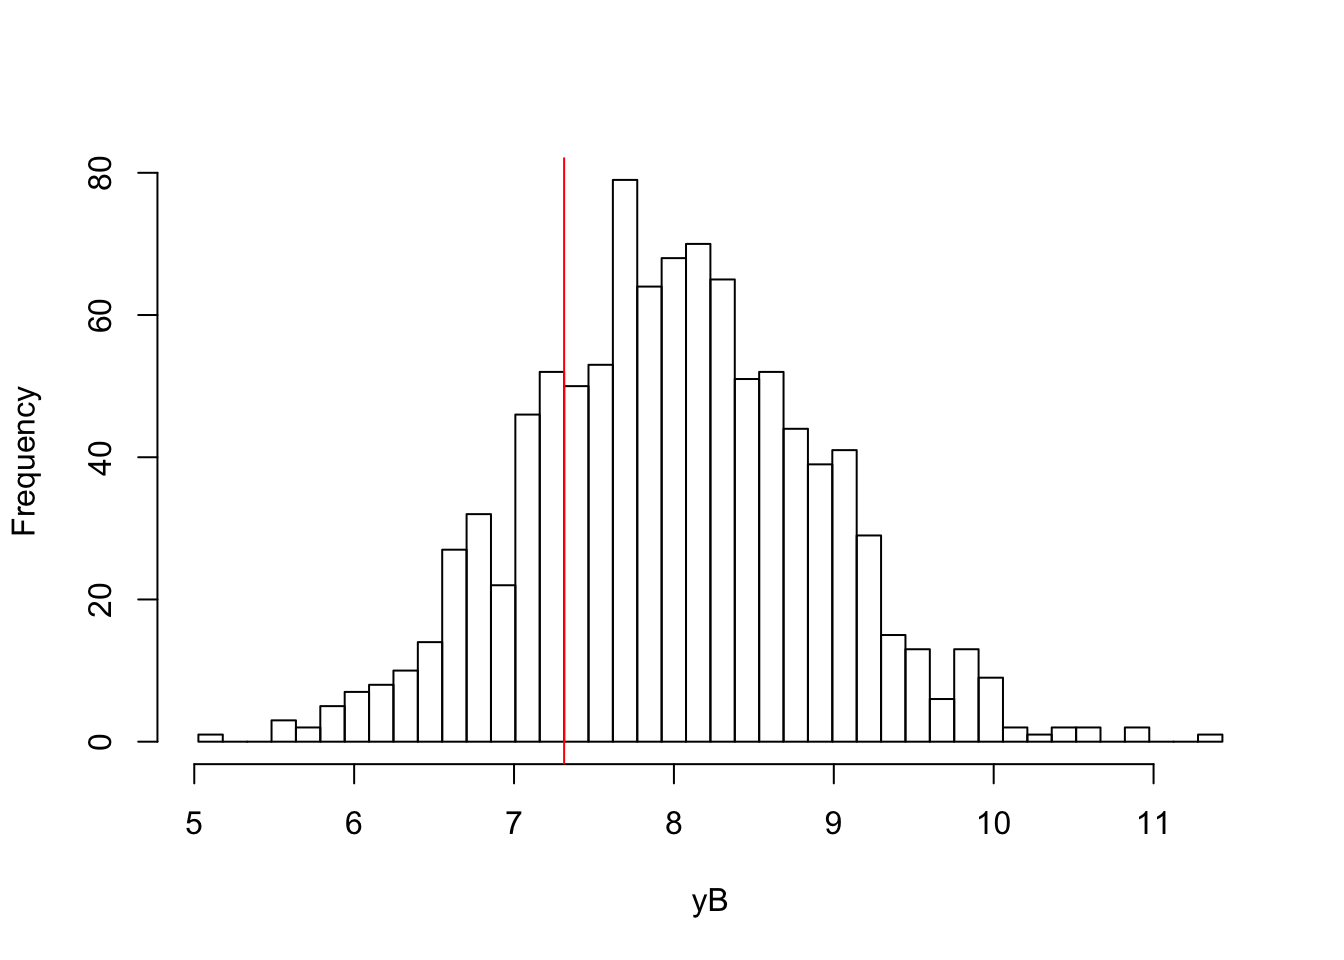
\includegraphics[width=0.6\linewidth]{STCI_files/figure-latex/histyb-1} 

}

\caption{Histogram of $y_B$}\label{fig:histyb}
\end{figure}

You can see on Figure \ref{fig:histyb} a histogram of \(y_i^B\) with the red line indicating the cutoff point: \(\bar{y}=\ln(\bar{Y})=\) 7.3.
All the observations below the red line are treated according to the sharp rule while all the one located above are not.
In order to see how many observations eventually receive the treatment with this allocation rule, let's build a contingency table.

\begin{Shaded}
\begin{Highlighting}[]
\NormalTok{table.D.sharp <-}\StringTok{ }\KeywordTok{as.matrix}\NormalTok{(}\KeywordTok{table}\NormalTok{(Ds))}
\NormalTok{knitr}\OperatorTok{::}\KeywordTok{kable}\NormalTok{(table.D.sharp,}\DataTypeTok{caption=}\StringTok{'Treatment allocation with sharp cutoff rule'}\NormalTok{,}\DataTypeTok{booktabs=}\OtherTok{TRUE}\NormalTok{)}
\end{Highlighting}
\end{Shaded}

\begin{table}[t]

\caption{\label{tab:tableDsharp}Treatment allocation with sharp cutoff rule}
\centering
\begin{tabular}{lr}
\toprule
0 & 771\\
1 & 229\\
\bottomrule
\end{tabular}
\end{table}

We can see on Table \ref{tab:tableDsharp} that there are 229 treated observations.

\hypertarget{fuzzy-cutoff-rule}{%
\subsubsection{Fuzzy cutoff rule}\label{fuzzy-cutoff-rule}}

This rule is less sharp than the sharp cutoff rule.
Here, other criteria than \(Y_i^B\) enter into the decision to allocate the treatment.
The doctor might measure the health status of a patient following official guidelines, but he might also measure other factors that will also influence his decision of giving the drug to the patient.
The officials administering a program might measure the official income level of a household, but they might also consider other features of the household situation when deciding to enroll the household into the program or not.
If these additional criteria are unobserved to the econometrician, then we have the fuzzy cutoff rule.
A very simple way to model this rule is as follows:

\begin{align}\label{eq:fuzzcutoff}
  D_i & = \uns{Y_i^B+V_i\leq\bar{Y}},
\end{align}

where \(V_i\) is a random variable unobserved to the econometrician and standing for the other influences that might drive the allocation of the treatment.
\(V_i\) is distributed according to a, for the moment, unspecified cumulative distribution function \(F_V\).
When \(V_i\) is degenerate (\textit{i.e.} it has only one point of support: it is a constant), the fuzzy cutoff rule becomes the sharp cutoff rule.

\hypertarget{eligibility-self-selection-rule}{%
\subsubsection{\texorpdfstring{Eligibility \(+\) self-selection rule}{Eligibility + self-selection rule}}\label{eligibility-self-selection-rule}}

It is also possible that households, once they have been made eligible to the treatment, can decide whether they want to receive it or not.
A patient might be able to refuse the drug that the doctor suggests she should take.
A household might refuse to participate in a cash transfer program to which it has been made eligible.
Not all programs have this feature, but most of them have some room for decisions by the agents themselves of whether they want to receive the treatment or not.
One simple way to model this rule is as follows:

\begin{align}\label{eq:eligself}
  D_i & = \uns{D^*_i\geq0}E_i,
\end{align}

where \(D^*_i\) is individual \(i\)'s valuation of the treatment and \(E_i\) is whether or not she is deemed eligible for the treatment.
\(E_i\) might be choosen according to the sharp cutoff rule of to the fuzzy cutoff rule, or to any other eligibility rule.
We will be more explicit about \(D_i^*\) in what follows.

\textbf{SIMULATIONS ARE MISSING FOR THESE LAST TWO RULES}

\hypertarget{potential-outcomes}{%
\subsection{Potential outcomes}\label{potential-outcomes}}

The second main building block of RCM are potential outcomes.
Let's say that we are interested in the effect of a treatment on an outcome \(Y\).
Each unit \(i\) can thus be in two potential states: treated or non treated.
Before the allocation of the treatment is decided, both of these states are feasible for each unit.

\BeginKnitrBlock{definition}[Potential outcomes]
\protect\hypertarget{def:unnamed-chunk-2}{}{\label{def:unnamed-chunk-2} \iffalse (Potential outcomes) \fi{} }For each unit \(i\), we define two potential outcomes:
\EndKnitrBlock{definition}

\begin{itemize}
\tightlist
\item
  \(Y_i^1\): the outcome that unit \(i\) is going to have if it receives the treatment,
\item
  \(Y_i^0\): the outcome that unit \(i\) is going to have if it \textbf{does not} receive the treatment.
\end{itemize}

\BeginKnitrBlock{example}
\protect\hypertarget{exm:unnamed-chunk-3}{}{\label{exm:unnamed-chunk-3} }Let's choose functional forms for our potential outcomes.
For simplicity, all lower case letters will denote log outcomes.
\(y_i^0=\mu_i+\delta+U_i^0\), with \(\delta\) a time shock common to all the observations and \(U_i^0=\rho U_i^B+\epsilon_i\), with \(|\rho|<1\).
In the absence of the treatment, part of the shocks \(U_i^B\) that the individuals experienced in the previous period persist, while some part vanish.
\(y_i^1=y_i^0+\bar{\alpha}+\theta\mu_i+\eta_i\).
In order to generate the potential outcomes, one has to define the laws for the shocks and to choose parameter values.
Let's assume that \(\epsilon_i\sim\mathcal{N}(0,\sigma^2_{\epsilon})\) and \(\eta_i\sim\mathcal{N}(0,\sigma^2_{\eta})\).
Now let's choose some parameter values:
\EndKnitrBlock{example}

\begin{Shaded}
\begin{Highlighting}[]
\NormalTok{l <-}\StringTok{ }\KeywordTok{length}\NormalTok{(param)}
\NormalTok{param <-}\StringTok{ }\KeywordTok{c}\NormalTok{(param,}\FloatTok{0.9}\NormalTok{,}\FloatTok{0.01}\NormalTok{,}\FloatTok{0.05}\NormalTok{,}\FloatTok{0.05}\NormalTok{,}\FloatTok{0.05}\NormalTok{,}\FloatTok{0.1}\NormalTok{)}
\KeywordTok{names}\NormalTok{(param)[(l}\OperatorTok{+}\DecValTok{1}\NormalTok{)}\OperatorTok{:}\KeywordTok{length}\NormalTok{(param)] <-}\StringTok{ }\KeywordTok{c}\NormalTok{(}\StringTok{"rho"}\NormalTok{,}\StringTok{"theta"}\NormalTok{,}\StringTok{"sigma2epsilon"}\NormalTok{,}\StringTok{"sigma2eta"}\NormalTok{,}\StringTok{"delta"}\NormalTok{,}\StringTok{"baralpha"}\NormalTok{)}
\NormalTok{param}
\end{Highlighting}
\end{Shaded}

\begin{verbatim}
##         barmu      sigma2mu       sigma2U          barY           rho 
##          8.00          0.50          0.28       1500.00          0.90 
##         theta sigma2epsilon     sigma2eta         delta      baralpha 
##          0.01          0.05          0.05          0.05          0.10
\end{verbatim}

We can finally generate the potential outcomes;

\begin{Shaded}
\begin{Highlighting}[]
\NormalTok{epsilon <-}\StringTok{ }\KeywordTok{rnorm}\NormalTok{(N,}\DecValTok{0}\NormalTok{,}\KeywordTok{sqrt}\NormalTok{(param[}\StringTok{"sigma2epsilon"}\NormalTok{]))}
\NormalTok{eta<-}\StringTok{ }\KeywordTok{rnorm}\NormalTok{(N,}\DecValTok{0}\NormalTok{,}\KeywordTok{sqrt}\NormalTok{(param[}\StringTok{"sigma2eta"}\NormalTok{]))}
\NormalTok{U0 <-}\StringTok{ }\NormalTok{param[}\StringTok{"rho"}\NormalTok{]}\OperatorTok{*}\NormalTok{UB }\OperatorTok{+}\StringTok{ }\NormalTok{epsilon}
\NormalTok{y0 <-}\StringTok{ }\NormalTok{mu }\OperatorTok{+}\StringTok{  }\NormalTok{U0 }\OperatorTok{+}\StringTok{ }\NormalTok{param[}\StringTok{"delta"}\NormalTok{]}
\NormalTok{alpha <-}\StringTok{ }\NormalTok{param[}\StringTok{"baralpha"}\NormalTok{]}\OperatorTok{+}\StringTok{  }\NormalTok{param[}\StringTok{"theta"}\NormalTok{]}\OperatorTok{*}\NormalTok{mu }\OperatorTok{+}\StringTok{ }\NormalTok{eta}
\NormalTok{y1 <-}\StringTok{ }\NormalTok{y0}\OperatorTok{+}\NormalTok{alpha}
\NormalTok{Y0 <-}\StringTok{ }\KeywordTok{exp}\NormalTok{(y0)}
\NormalTok{Y1 <-}\StringTok{ }\KeywordTok{exp}\NormalTok{(y1)}
\end{Highlighting}
\end{Shaded}

Now, I would like to visualize my potential outcomes:

\begin{Shaded}
\begin{Highlighting}[]
\KeywordTok{plot}\NormalTok{(y0,y1)}
\end{Highlighting}
\end{Shaded}

\begin{figure}

{\centering 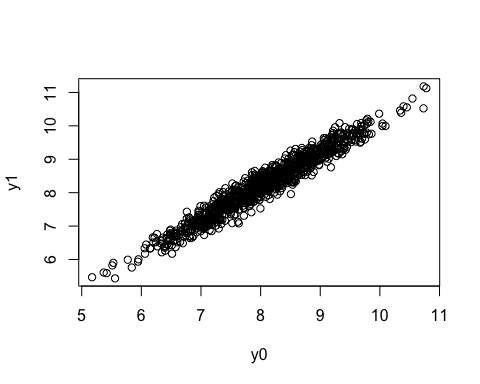
\includegraphics[width=0.6\linewidth]{STCI_files/figure-latex/histpotout-1} 

}

\caption{Potential outcomes}\label{fig:histpotout}
\end{figure}

You can see on the resulting Figure \ref{fig:histpotout} that both potential outcomes are positively correlated.
Those with a large potential outcome when untreated (\emph{e.g.} in good health without the treatment) also have a positive health with the treatment.
It is also true that individuals with bad health in the absence of the treatment also have bad health with the treatment.

\hypertarget{switching-equation}{%
\subsection{Switching equation}\label{switching-equation}}

The last building block of RCM is the switching equation.
It links the observed outcome to the potential outcomes through the allocation rule:

\begin{align}
 \label{eq:switch}
  Y_i & = 
    \begin{cases}
    Y_i^1 & \text{if } D_i=1\\
    Y_i^0 & \text{if } D_i=0
    \end{cases} \\
    & = Y_i^1D_i + Y_i^0(1-D_i) \nonumber
\end{align}

\BeginKnitrBlock{example}
\protect\hypertarget{exm:unnamed-chunk-4}{}{\label{exm:unnamed-chunk-4} }In order to generate observed outcomes in our numerical example, we simply have to enforce the switching equation:
\EndKnitrBlock{example}

\begin{Shaded}
\begin{Highlighting}[]
\NormalTok{y <-}\StringTok{ }\NormalTok{y1}\OperatorTok{*}\NormalTok{Ds}\OperatorTok{+}\NormalTok{y0}\OperatorTok{*}\NormalTok{(}\DecValTok{1}\OperatorTok{-}\NormalTok{Ds)}
\NormalTok{Y <-}\StringTok{ }\NormalTok{Y1}\OperatorTok{*}\NormalTok{Ds}\OperatorTok{+}\NormalTok{Y0}\OperatorTok{*}\NormalTok{(}\DecValTok{1}\OperatorTok{-}\NormalTok{Ds)}
\end{Highlighting}
\end{Shaded}

What the switching equation \eqref{eq:switch} means is that, for each individual \(i\), we get to observe only one of the two potential outcomes.
When individual \(i\) belongs to the treatment group (\emph{i.e.} \(D_i=1\)), we get to observe \(Y_i^1\).
When individual \(i\) belongs to the control group (\emph{i.e.} \(D_i=0\)), we get to observe \(Y_i^0\).
Because the same individual cannot be at the same time in both groups, we can NEVER see both potential outcomes for the same individual at the same time.

For each of the individuals, one of the two potential outcomes is unobserved.
We say that it is a \textbf{counterfactual}.
A counterfactual quantity is a quantity that is, according to Hume's definition, contrary to the observed facts.
A counterfactual cannot be observed, but it can be conceived by an effort of reason: it is the consequence of what would have happened had some action not been taken.

\BeginKnitrBlock{remark}
\iffalse{} {Remark. } \fi{}One very nice way of visualising the switching equation has been proposed by Jerzy Neyman in a 1923 prescient paper.
Neyman proposes to imagine two urns, each one filled with \(N\) balls.
One urn is the treatment urn and contains balls with the id of the unit and the value of its potential outcome \(Y_i^1\).
The other urn is the control urn, and it contains balls with the value of the potential outcome \(Y_i^0\) for each unit \(i\).
Following the allocation rule \(D_i\), we decide whether unit \(i\) is in the treatment or control group.
When unit \(i\) is in the treatment group, we take the corresponding ball from the first urn and observe the potential outcome on it.
But, at the same time, the urns are connected so that the corresponding ball with the potential outcome of unit \(i\) in the control urn disappears as soon as we draw ball \(i\) from the treatment urn.

The switching equation works a lot like Schrodinger's cat paradox.
Schrodinger's cat is placed in a sealed box and receives a dose of poison when an atom emits a radiation.
As long as the box is sealed, there is no way we can know whether the cat is dead or alive.
When we open the box, we observe either a dead cat or a living cat, but we cannot observe the cat both alive and dead at the same time.
The switching equation is like opening the box, it collapses the observed outcome into one of the two potential ones.
\EndKnitrBlock{remark}

\BeginKnitrBlock{example}
\protect\hypertarget{exm:unnamed-chunk-6}{}{\label{exm:unnamed-chunk-6} }One way to visualize the inner workings of the switching equation is to plot the potential outcomes along with the criteria driving the allocation rule.
In our simple example, it simply amounts to plotting observed (\(y_i\)) and potential outcomes (\(y_i^1\) and \(y_i^0\)) along \(y_i^B\).
\EndKnitrBlock{example}

\begin{Shaded}
\begin{Highlighting}[]
\KeywordTok{plot}\NormalTok{(yB[Ds}\OperatorTok{==}\DecValTok{0}\NormalTok{],y0[Ds}\OperatorTok{==}\DecValTok{0}\NormalTok{],}\DataTypeTok{pch=}\DecValTok{1}\NormalTok{,}\DataTypeTok{xlim=}\KeywordTok{c}\NormalTok{(}\DecValTok{5}\NormalTok{,}\DecValTok{11}\NormalTok{),}\DataTypeTok{ylim=}\KeywordTok{c}\NormalTok{(}\DecValTok{5}\NormalTok{,}\DecValTok{11}\NormalTok{),}\DataTypeTok{xlab=}\StringTok{"yB"}\NormalTok{,}\DataTypeTok{ylab=}\StringTok{"Outcomes"}\NormalTok{)}
\KeywordTok{points}\NormalTok{(yB[Ds}\OperatorTok{==}\DecValTok{1}\NormalTok{],y1[Ds}\OperatorTok{==}\DecValTok{1}\NormalTok{],}\DataTypeTok{pch=}\DecValTok{3}\NormalTok{)}
\KeywordTok{points}\NormalTok{(yB[Ds}\OperatorTok{==}\DecValTok{0}\NormalTok{],y1[Ds}\OperatorTok{==}\DecValTok{0}\NormalTok{],}\DataTypeTok{pch=}\DecValTok{3}\NormalTok{,}\DataTypeTok{col=}\StringTok{'red'}\NormalTok{)}
\KeywordTok{points}\NormalTok{(yB[Ds}\OperatorTok{==}\DecValTok{1}\NormalTok{],y0[Ds}\OperatorTok{==}\DecValTok{1}\NormalTok{],}\DataTypeTok{pch=}\DecValTok{1}\NormalTok{,}\DataTypeTok{col=}\StringTok{'red'}\NormalTok{)}
\NormalTok{test <-}\StringTok{ }\FloatTok{5.8}
\NormalTok{i.test <-}\StringTok{ }\KeywordTok{which}\NormalTok{(}\KeywordTok{abs}\NormalTok{(yB}\OperatorTok{-}\NormalTok{test)}\OperatorTok{==}\KeywordTok{min}\NormalTok{(}\KeywordTok{abs}\NormalTok{(yB}\OperatorTok{-}\NormalTok{test)))}
\KeywordTok{points}\NormalTok{(yB[}\KeywordTok{abs}\NormalTok{(yB}\OperatorTok{-}\NormalTok{test)}\OperatorTok{==}\KeywordTok{min}\NormalTok{(}\KeywordTok{abs}\NormalTok{(yB}\OperatorTok{-}\NormalTok{test))],y1[}\KeywordTok{abs}\NormalTok{(yB}\OperatorTok{-}\NormalTok{test)}\OperatorTok{==}\KeywordTok{min}\NormalTok{(}\KeywordTok{abs}\NormalTok{(yB}\OperatorTok{-}\NormalTok{test))],}\DataTypeTok{col=}\StringTok{'green'}\NormalTok{,}\DataTypeTok{pch=}\DecValTok{3}\NormalTok{)}
\KeywordTok{points}\NormalTok{(yB[}\KeywordTok{abs}\NormalTok{(yB}\OperatorTok{-}\NormalTok{test)}\OperatorTok{==}\KeywordTok{min}\NormalTok{(}\KeywordTok{abs}\NormalTok{(yB}\OperatorTok{-}\NormalTok{test))],y0[}\KeywordTok{abs}\NormalTok{(yB}\OperatorTok{-}\NormalTok{test)}\OperatorTok{==}\KeywordTok{min}\NormalTok{(}\KeywordTok{abs}\NormalTok{(yB}\OperatorTok{-}\NormalTok{test))],}\DataTypeTok{col=}\StringTok{'green'}\NormalTok{)}
\KeywordTok{abline}\NormalTok{(}\DataTypeTok{v=}\KeywordTok{log}\NormalTok{(param[}\StringTok{"barY"}\NormalTok{]),}\DataTypeTok{col=}\StringTok{"red"}\NormalTok{)}
\KeywordTok{legend}\NormalTok{(}\DecValTok{5}\NormalTok{,}\DecValTok{11}\NormalTok{,}\KeywordTok{c}\NormalTok{(}\StringTok{'y0|D=0'}\NormalTok{,}\StringTok{'y1|D=1'}\NormalTok{,}\StringTok{'y0|D=1'}\NormalTok{,}\StringTok{'y1|D=0'}\NormalTok{,}\KeywordTok{paste}\NormalTok{(}\StringTok{'y0'}\NormalTok{,i.test,}\DataTypeTok{sep=}\StringTok{''}\NormalTok{),}\KeywordTok{paste}\NormalTok{(}\StringTok{'y1'}\NormalTok{,i.test,}\DataTypeTok{sep=}\StringTok{''}\NormalTok{)),}\DataTypeTok{pch=}\KeywordTok{c}\NormalTok{(}\DecValTok{1}\NormalTok{,}\DecValTok{3}\NormalTok{,}\DecValTok{1}\NormalTok{,}\DecValTok{3}\NormalTok{,}\DecValTok{1}\NormalTok{,}\DecValTok{3}\NormalTok{),}\DataTypeTok{col=}\KeywordTok{c}\NormalTok{(}\StringTok{'black'}\NormalTok{,}\StringTok{'black'}\NormalTok{,}\StringTok{'red'}\NormalTok{,}\StringTok{'red'}\NormalTok{,}\StringTok{'green'}\NormalTok{,}\StringTok{'green'}\NormalTok{),}\DataTypeTok{ncol=}\DecValTok{3}\NormalTok{)}
\end{Highlighting}
\end{Shaded}

\begin{figure}

{\centering 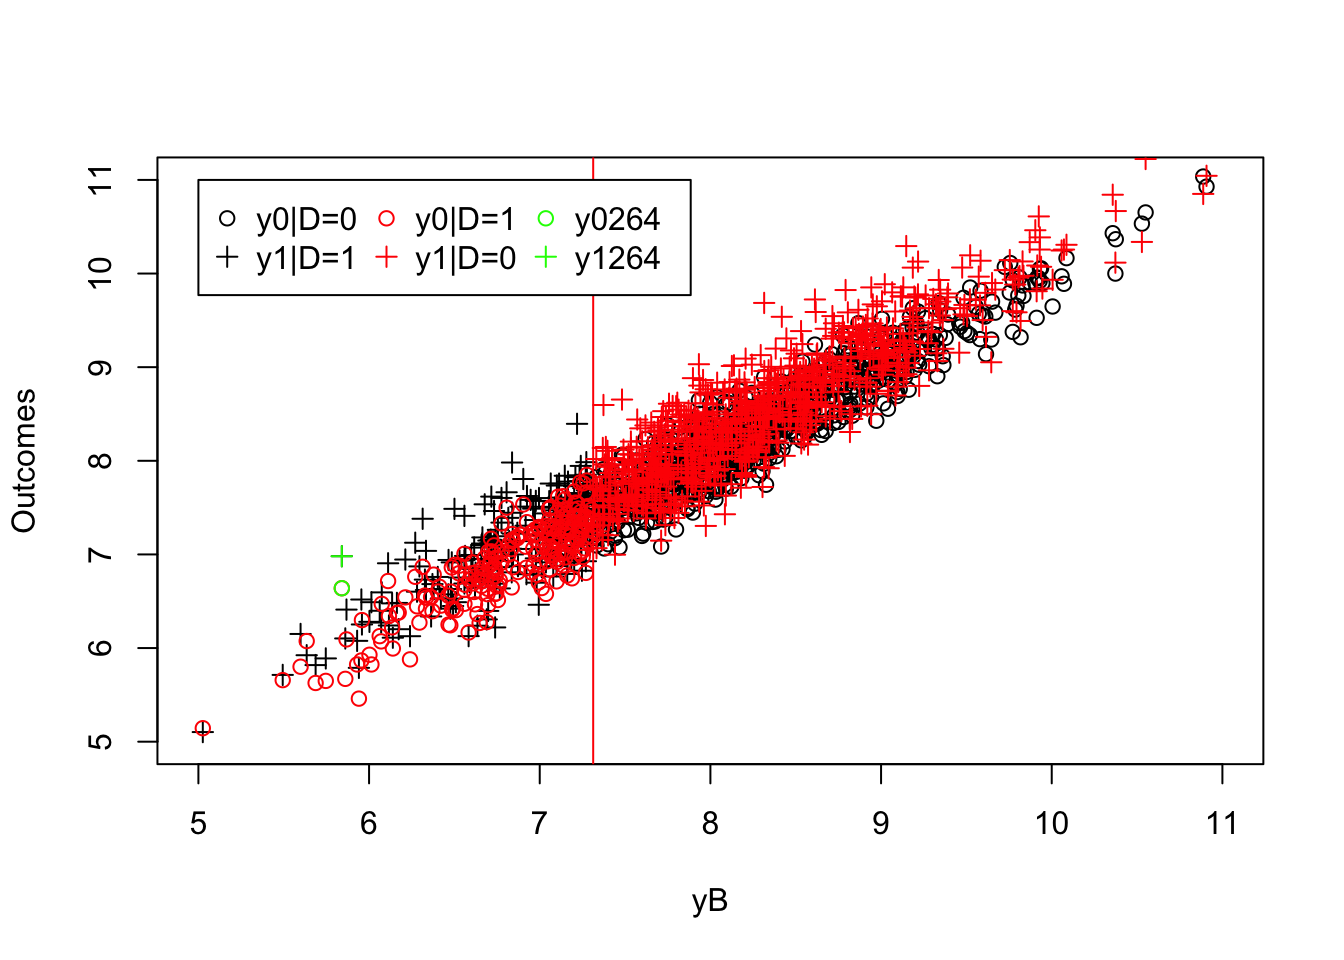
\includegraphics[width=0.6\linewidth]{STCI_files/figure-latex/ploty1y0yB-1} 

}

\caption{Potential outcomes}\label{fig:ploty1y0yB}
\end{figure}

\begin{Shaded}
\begin{Highlighting}[]
\KeywordTok{plot}\NormalTok{(yB[Ds}\OperatorTok{==}\DecValTok{0}\NormalTok{],y0[Ds}\OperatorTok{==}\DecValTok{0}\NormalTok{],}\DataTypeTok{pch=}\DecValTok{1}\NormalTok{,}\DataTypeTok{xlim=}\KeywordTok{c}\NormalTok{(}\DecValTok{5}\NormalTok{,}\DecValTok{11}\NormalTok{),}\DataTypeTok{ylim=}\KeywordTok{c}\NormalTok{(}\DecValTok{5}\NormalTok{,}\DecValTok{11}\NormalTok{),}\DataTypeTok{xlab=}\StringTok{"yB"}\NormalTok{,}\DataTypeTok{ylab=}\StringTok{"Outcomes"}\NormalTok{)}
\KeywordTok{points}\NormalTok{(yB[Ds}\OperatorTok{==}\DecValTok{1}\NormalTok{],y1[Ds}\OperatorTok{==}\DecValTok{1}\NormalTok{],}\DataTypeTok{pch=}\DecValTok{3}\NormalTok{)}
\KeywordTok{legend}\NormalTok{(}\DecValTok{5}\NormalTok{,}\DecValTok{11}\NormalTok{,}\KeywordTok{c}\NormalTok{(}\StringTok{'y|D=0'}\NormalTok{,}\StringTok{'y|D=1'}\NormalTok{),}\DataTypeTok{pch=}\KeywordTok{c}\NormalTok{(}\DecValTok{1}\NormalTok{,}\DecValTok{3}\NormalTok{))}
\KeywordTok{abline}\NormalTok{(}\DataTypeTok{v=}\KeywordTok{log}\NormalTok{(param[}\StringTok{"barY"}\NormalTok{]),}\DataTypeTok{col=}\StringTok{"red"}\NormalTok{)}
\end{Highlighting}
\end{Shaded}

\begin{figure}

{\centering 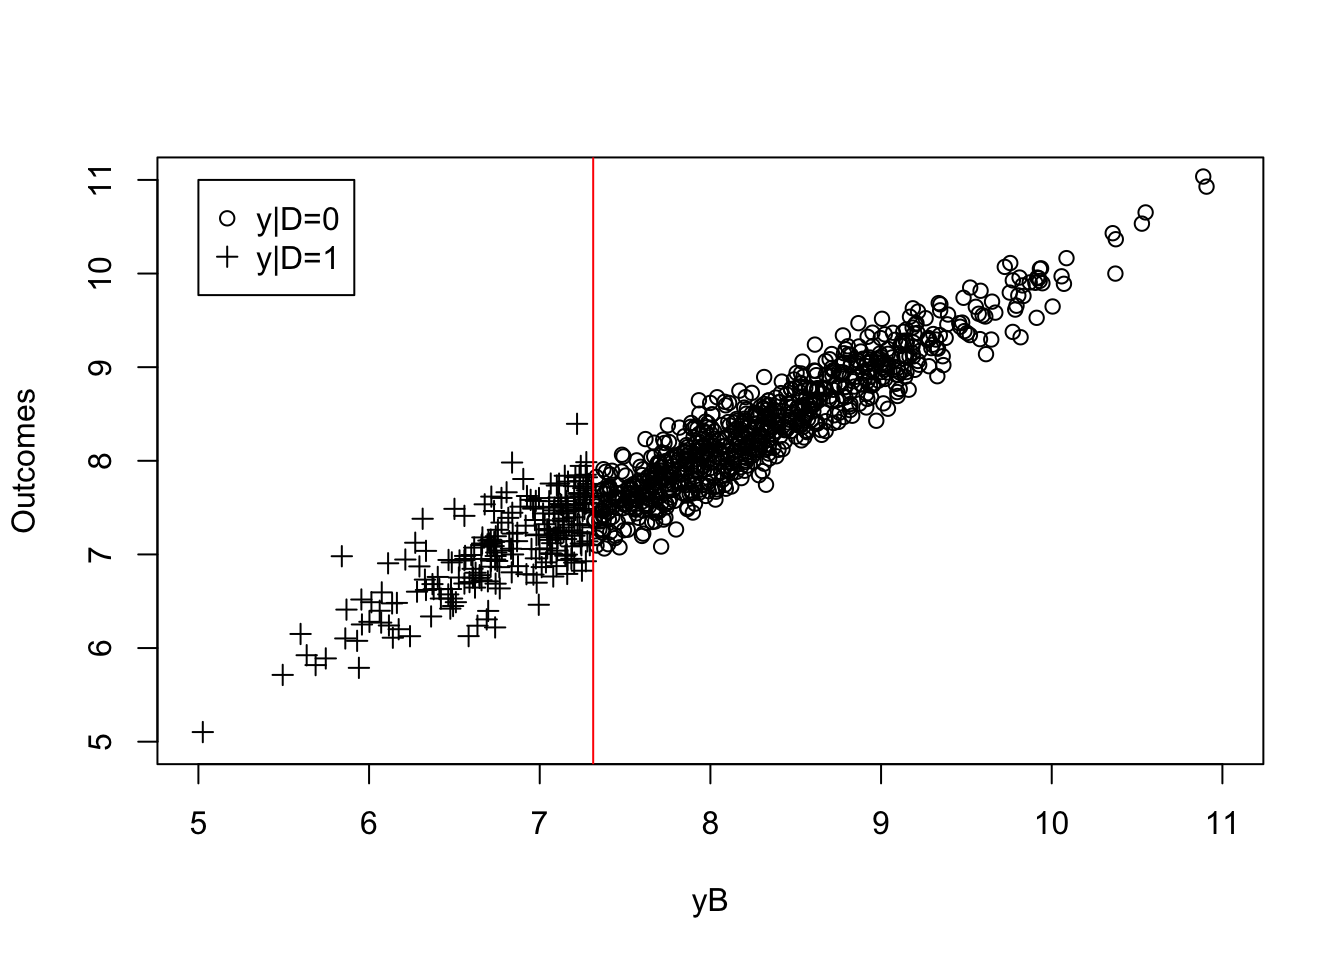
\includegraphics[width=0.6\linewidth]{STCI_files/figure-latex/plotyyB-1} 

}

\caption{Observed outcomes}\label{fig:plotyyB}
\end{figure}

Figure \ref{fig:ploty1y0yB} plots the observed outcomes \(y_i\) along with the unobserved potential outcomes.
Figure \ref{fig:ploty1y0yB} shows that each individual in the sample is endowed with two potential outcomes, represented by a circle and a cross.
Figure \ref{fig:plotyyB} plots the observed outcomes \(y_i\) that results from applying the switching equation.
Only one of the two potential outcomes is observed (the cross for the treated group and the circle for the untreated group) and the other is not.
The observed sample in Figure \ref{fig:plotyyB} only shows observed outcomes, and is thus silent on the values of the missing potential outcomes.

\hypertarget{treatment-effects}{%
\section{Treatment effects}\label{treatment-effects}}

RCM enables the definition of causal effects at the individual level.
In practice though, we generally focus on a summary measure: the effect of the treatment on the treated.

\hypertarget{individual-level-treatment-effects}{%
\subsection{Individual level treatment effects}\label{individual-level-treatment-effects}}

Potential outcomes enable us to define the central notion of causal inference: the causal effect, also labelled the treatment effect, which is the difference between the two potential outcomes.

\BeginKnitrBlock{definition}[Individual level treatment effect]
\protect\hypertarget{def:causaleff}{}{\label{def:causaleff} \iffalse (Individual level treatment effect) \fi{} }For each unit \(i\), the causal effect of the treatment on outcome \(Y\) is: \(\Delta^Y_i=Y_i^1-Y_i^0\).
\EndKnitrBlock{definition}

\BeginKnitrBlock{example}
\protect\hypertarget{exm:unnamed-chunk-7}{}{\label{exm:unnamed-chunk-7} }The individual level causal effect in log terms is: \(\Delta^y_i=\alpha_i=\bar{\alpha}+\theta\mu_i+\eta_i\).
The effect is the sum of a part common to all individuals, a part correlated with \(\mu_i\): the treatment might have a larger or a smaller effect depending on the unobserved permanent ability or health status of individuals, and a random shock.
It is possible to make the effect of the treatment to depend on \(U_i^B\) also, but it would complicate the model.
\EndKnitrBlock{example}

In Figure \ref{fig:ploty1y0yB}, the individual level treatment effects are the differences between each cross and its corresponding circle.
For example, for observation 264, the two potential outcomes appear in green in Figure \ref{fig:ploty1y0yB}.
The effect of the treatment on unit 264 is equal to:
\[
\Delta^y_{264}=y^1_{264}-y^0_{264}=6.98-6.64=0.34.
\]

Since observation 264 belongs to the treatment group, we can only observe the potential outcome in the presence of the treatment, \(y^1_{264}\).

RCM allows for heterogeneity of treatment effects.
The treatment has a large effect on some units and a much smaller effect on other units.
We can even have some units that benefit from the treatment and some units that are harmed by the treatment.
The individual level effect of the treatment is itself a random variable (and not a fixed parameter).
It has a distribution, \(F_{\Delta^Y}\).

Heterogeneity of treatment effects seems very natural: the treatment might interact with individuals' different backgrounds.
The effect of a drug might depend on the genetic background of an individual.
An education program might only work for children that already have sufficient non-cognitive skills, and thus might depend in turn on family background.
An environmental regulation or a behavioral intervention might only trigger reactions by already environmentally aware individuals.
A CCT might have a larger effect when indiviuals are credit-constrained or face shocks.

\BeginKnitrBlock{example}
\protect\hypertarget{exm:unnamed-chunk-8}{}{\label{exm:unnamed-chunk-8} }In our numerical example, the distribution of \(\Delta^y_i=\alpha_i\) is a normal: \(\alpha_i\sim\mathcal{N}(\bar{\alpha}+\theta\bar{\mu},\theta^2\sigma^2_{\mu}+\sigma^2_{\eta})\).
We would like to visualize treatment effect heterogeneity.
For that, we can build a histogram of the individual level causal effect.
\EndKnitrBlock{example}

On top of the histogram, we can also draw the theoretical distribution of the treatment effect: a normal with mean 0.18 and variance 0.05.

\begin{Shaded}
\begin{Highlighting}[]
\KeywordTok{hist}\NormalTok{(alpha,}\DataTypeTok{main=}\StringTok{""}\NormalTok{,}\DataTypeTok{prob=}\OtherTok{TRUE}\NormalTok{)}
\KeywordTok{curve}\NormalTok{(}\KeywordTok{dnorm}\NormalTok{(x, }\DataTypeTok{mean=}\NormalTok{(param[}\StringTok{"baralpha"}\NormalTok{]}\OperatorTok{+}\NormalTok{param[}\StringTok{"theta"}\NormalTok{]}\OperatorTok{*}\NormalTok{param[}\StringTok{"barmu"}\NormalTok{]), }\DataTypeTok{sd=}\KeywordTok{sqrt}\NormalTok{(param[}\StringTok{"theta"}\NormalTok{]}\OperatorTok{^}\DecValTok{2}\OperatorTok{*}\NormalTok{param[}\StringTok{"sigma2mu"}\NormalTok{]}\OperatorTok{+}\NormalTok{param[}\StringTok{"sigma2eta"}\NormalTok{])), }\DataTypeTok{add=}\OtherTok{TRUE}\NormalTok{,}\DataTypeTok{col=}\StringTok{'red'}\NormalTok{)}
\end{Highlighting}
\end{Shaded}

\begin{figure}[htbp]

{\centering 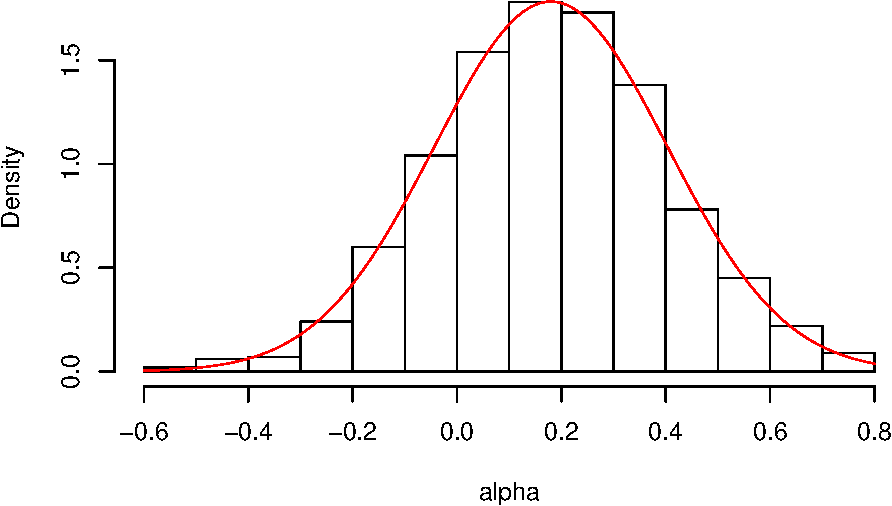
\includegraphics[width=0.6\linewidth]{STCI_files/figure-latex/histalpha-1} 

}

\caption{Histogram of $\Delta^y$}\label{fig:histalpha}
\end{figure}

The first thing that we can see on Figure \ref{fig:histalpha} is that the theoretical and the empirical distributions nicely align with each other.
We also see that the majority of the observations lies to the right of zero: most people experience a positive effect of the treatment.
But there are some individuals that do not benefit from the treatment: the effect of the treatment on them is negative.

\hypertarget{average-treatment-effect-on-the-treated}{%
\subsection{Average treatment effect on the treated}\label{average-treatment-effect-on-the-treated}}

We do not generally estimate individual-level treatment effects.
We generally look for summary statistics of the effect of the treatment.
By far the most widely reported causal parameter is the Treatment on the Treated parameter (TT).
It can be defined in the sample at hand or in the population.

\BeginKnitrBlock{definition}[Average and expected treatment effects on the treated]
\protect\hypertarget{def:TT}{}{\label{def:TT} \iffalse (Average and expected treatment effects on the treated) \fi{} }The Treatment on the Treated parameters for outcome \(Y\) are:
\EndKnitrBlock{definition}

\begin{itemize}
\item
  The average Treatment effect on the Treated in the sample:

  \begin{align*}
  \Delta^Y_{TT_s} & = \frac{1}{\sum_{i=1}^ND_i}\sum_{i=1}^N(Y_i^1-Y_i^0)D_i,
  \end{align*}
\item
  The expected Treatment effect on the Treated in the population:

  \begin{align*}
  \Delta^Y_{TT} & = \esp{Y_i^1-Y_i^0|D_i=1}.
  \end{align*}
\end{itemize}

The TT parameters measure the average effect of the treatment on those who actually take it, either in the sample at hand or in the popluation.
It is generally considered to be the most policy-relevant parameter since it measures the effect of the treatment as it has actually been allocated.
For example, the expected causal effect on the overall population is only relevant if policymakers are considering implementing the treatment even on those who have not been selected to receive it.
For a drug or an anti-poverty program, it would mean giving the treatment to healthy or rich people, which would make little sense.

TT does not say anything about how the effect of the treatment is distributed in the population or in the sample.
TT does not account for the heterogneity of treatment effects.
In Lecture 7, we will look at other parameters of interest that look more closely into how the effect of the treatment is distributed.

\BeginKnitrBlock{example}
\protect\hypertarget{exm:unnamed-chunk-9}{}{\label{exm:unnamed-chunk-9} }The value of TT in our sample is:
\EndKnitrBlock{example}

\[
\Delta^y_{TT_s}=0.168.
\]

Computing the population value of \(TT\) is slightly more involved: we have to use the formula for the conditional expectation of a censored bivariate normal random variable:

\begin{align*}
\Delta^y_{TT} & = \esp{\alpha_i|D_i=1}\\
              & = \bar{\alpha}+\theta\esp{\mu_i|\mu_i+U_i^B\leq\bar{y}}\\
              & = \bar{\alpha}+\theta\left(\bar{\mu} - \frac{\sigma^2_{\mu}}{\sqrt{\sigma^2_{\mu}+\sigma^2_{U}}}\frac{\phi\left(\frac{\bar{y}-\bar{\mu}}{\sqrt{\sigma^2_{\mu}+\sigma^2_{U}}}\right)}{\Phi\left(\frac{\bar{y}-\bar{\mu}}{\sqrt{\sigma^2_{\mu}+\sigma^2_{U}}}\right)}\right)\\
              & = \bar{\alpha}+\theta\bar{\mu}-\theta\left(\frac{\sigma^2_{\mu}}{\sqrt{\sigma^2_{\mu}+\sigma^2_{U}}}\frac{\phi\left(\frac{\bar{y}-\bar{\mu}}{\sqrt{\sigma^2_{\mu}+\sigma^2_{U}}}\right)}{\Phi\left(\frac{\bar{y}-\bar{\mu}}{\sqrt{\sigma^2_{\mu}+\sigma^2_{U}}}\right)}\right),
\end{align*}

where \(\phi\) and \(\Phi\) are respectively the density and the cumulative distribution functions of the standard normal.
The second equality follows from the definition of \(\alpha_i\) and \(D_i\) and from the fact that \(\eta_i\) is independent from \(\mu_i\) and \(U_i^B\).
The third equality comes from the formula for the expectation of a censored bivariate normal random variable.
In order to compute the population value of TT easily for different sets of parameter values, let's write a function in R:

\begin{Shaded}
\begin{Highlighting}[]
\NormalTok{delta.y.tt <-}\StringTok{ }\ControlFlowTok{function}\NormalTok{(param)\{}\KeywordTok{return}\NormalTok{(param[}\StringTok{"baralpha"}\NormalTok{]}\OperatorTok{+}\NormalTok{param[}\StringTok{"theta"}\NormalTok{]}\OperatorTok{*}\NormalTok{param[}\StringTok{"barmu"}\NormalTok{]}
                                     \OperatorTok{-}\NormalTok{param[}\StringTok{"theta"}\NormalTok{]}\OperatorTok{*}\NormalTok{((param[}\StringTok{"sigma2mu"}\NormalTok{]}\OperatorTok{*}\KeywordTok{dnorm}\NormalTok{((}\KeywordTok{log}\NormalTok{(param[}\StringTok{"barY"}\NormalTok{])}\OperatorTok{-}\NormalTok{param[}\StringTok{"barmu"}\NormalTok{])}\OperatorTok{/}\NormalTok{(}\KeywordTok{sqrt}\NormalTok{(param[}\StringTok{"sigma2mu"}\NormalTok{]}\OperatorTok{+}\NormalTok{param[}\StringTok{"sigma2U"}\NormalTok{]))))}
                                                      \OperatorTok{/}\NormalTok{(}\KeywordTok{sqrt}\NormalTok{(param[}\StringTok{"sigma2mu"}\NormalTok{]}\OperatorTok{+}\NormalTok{param[}\StringTok{"sigma2U"}\NormalTok{])}
                                                        \OperatorTok{*}\KeywordTok{pnorm}\NormalTok{((}\KeywordTok{log}\NormalTok{(param[}\StringTok{"barY"}\NormalTok{])}\OperatorTok{-}\NormalTok{param[}\StringTok{"barmu"}\NormalTok{])}\OperatorTok{/}\NormalTok{(}\KeywordTok{sqrt}\NormalTok{(param[}\StringTok{"sigma2mu"}\NormalTok{]}\OperatorTok{+}\NormalTok{param[}\StringTok{"sigma2U"}\NormalTok{]))))))\}}
\end{Highlighting}
\end{Shaded}

The population value of TT computed using this function is: \(\Delta^y_{TT}=\) 0.172.
We can see that the values of TT in the sample and in the population differ slightly.
This is because of sampling noise: the units in the sample are not perfectly representative of the units in the population.

\hypertarget{fundamental-problem-of-causal-inference}{%
\section{Fundamental problem of causal inference}\label{fundamental-problem-of-causal-inference}}

At least in this lecture, causal inference is about trying to infer TT, either in the sample or in the population.
The FPCI states that it is impossible to directly observe TT because one part of it remains fundamentally unobserved.

\BeginKnitrBlock{theorem}[Fundamental problem of causal inference]
\protect\hypertarget{thm:FPCI}{}{\label{thm:FPCI} \iffalse (Fundamental problem of causal inference) \fi{} }It is impossible to observe TT, either in the population or in the sample.
\EndKnitrBlock{theorem}

\BeginKnitrBlock{proof}
\iffalse{} {Proof. } \fi{}The proof of the FPCI is rather straightforward.
Let me start with the sample TT:

\begin{align*}
  \Delta^Y_{TT_s} & = \frac{1}{\sum_{i=1}^ND_i}\sum_{i=1}^N(Y_i^1-Y_i^0)D_i \\
                  & = \frac{1}{\sum_{i=1}^ND_i}\sum_{i=1}^NY_i^1D_i- \frac{1}{\sum_{i=1}^ND_i}\sum_{i=1}^NY_i^0D_i \\
                  & = \frac{1}{\sum_{i=1}^ND_i}\sum_{i=1}^NY_iD_i- \frac{1}{\sum_{i=1}^ND_i}\sum_{i=1}^NY_i^0D_i.
\end{align*}

Since \(Y_i^0\) is unobserved whenever \(D_i=1\), \(\frac{1}{\sum_{i=1}^ND_i}\sum_{i=1}^NY_i^0D_i\) is unobserved, and so is \(\Delta^Y_{TT_s}\).
The same is true for the population TT:

\begin{align*}
  \Delta^Y_{TT} & = \esp{Y_i^1-Y_i^0|D_i=1} \\
                & = \esp{Y_i^1|D_i=1}-\esp{Y_i^0|D_i=1}\\
                & = \esp{Y_i|D_i=1}-\esp{Y_i^0|D_i=1}.
\end{align*}

\(\esp{Y_i^0|D_i=1}\) is unobserved, and so is \(\Delta^Y_{TT}\).
\EndKnitrBlock{proof}

The key insight in order to understand the FPCI is to see that the outcomes of the treated units had they not been treated are unobservable, and so is their average or expectation.
We say that they are counterfactual, contrary to what has happened.

\BeginKnitrBlock{definition}[Couterfactual]
\protect\hypertarget{def:counter}{}{\label{def:counter} \iffalse (Couterfactual) \fi{} }Both \(\frac{1}{\sum_{i=1}^ND_i}\sum_{i=1}^NY_i^0D_i\) and \(\esp{Y_i^0|D_i=1}\) are counterfactual quantities that we will never get to observe.
\EndKnitrBlock{definition}

\BeginKnitrBlock{example}
\protect\hypertarget{exm:unnamed-chunk-11}{}{\label{exm:unnamed-chunk-11} }The average counterfactual outcome of the treated is the mean of the red circles in the \(y\) axis on Figure \ref{fig:ploty1y0yB}:
\EndKnitrBlock{example}

\[
\frac{1}{\sum_{i=1}^ND_i}\sum_{i=1}^Ny_i^0D_i= 6.91.
\]
Remember that we can estimate this quantity only because we have generated the data ourselves.
In real life, this quantity is hopelessly unobserved.

\(\esp{y_i^0|D_i=1}\) can be computed using the formula for the expectation of a censored normal random variable:

\begin{align*}
\esp{y_i^0|D_i=1} & = \esp{\mu_i+\delta+U_i^0|D_i=1}\\
                  & = \esp{\mu_i+\delta+\rho U_i^B+\epsilon_i|D_i=1}\\
                  & = \delta + \esp{\mu_i+\rho U_i^B|y_i^B\leq\bar{y}}\\
                  & = \delta + \bar{\mu} - \frac{\sigma^2_{\mu}+\rho\sigma^2_U}{\sqrt{\sigma^2_{\mu}+\sigma^2_{U}}}\frac{\phi\left(\frac{\bar{y}-\bar{\mu}}{\sqrt{\sigma^2_{\mu}+\sigma^2_{U}}}\right)}{\Phi\left(\frac{\bar{y}-\bar{\mu}}{\sqrt{\sigma^2_{\mu}+\sigma^2_{U}}}\right)}.
\end{align*}

We can write a function in R to compute this value:

\begin{Shaded}
\begin{Highlighting}[]
\NormalTok{esp.y0.D1 <-}\StringTok{ }\ControlFlowTok{function}\NormalTok{(param)\{}
  \KeywordTok{return}\NormalTok{(param[}\StringTok{"delta"}\NormalTok{]}\OperatorTok{+}\NormalTok{param[}\StringTok{"barmu"}\NormalTok{]}
         \OperatorTok{-}\NormalTok{((param[}\StringTok{"sigma2mu"}\NormalTok{]}\OperatorTok{+}\NormalTok{param[}\StringTok{"rho"}\NormalTok{]}\OperatorTok{*}\NormalTok{param[}\StringTok{"sigma2U"}\NormalTok{])}
           \OperatorTok{*}\KeywordTok{dnorm}\NormalTok{((}\KeywordTok{log}\NormalTok{(param[}\StringTok{"barY"}\NormalTok{])}\OperatorTok{-}\NormalTok{param[}\StringTok{"barmu"}\NormalTok{])}\OperatorTok{/}\NormalTok{(}\KeywordTok{sqrt}\NormalTok{(param[}\StringTok{"sigma2mu"}\NormalTok{]}\OperatorTok{+}\NormalTok{param[}\StringTok{"sigma2U"}\NormalTok{]))))}
         \OperatorTok{/}\NormalTok{(}\KeywordTok{sqrt}\NormalTok{(param[}\StringTok{"sigma2mu"}\NormalTok{]}\OperatorTok{+}\NormalTok{param[}\StringTok{"sigma2U"}\NormalTok{])}\OperatorTok{*}\KeywordTok{pnorm}\NormalTok{((}\KeywordTok{log}\NormalTok{(param[}\StringTok{"barY"}\NormalTok{])}\OperatorTok{-}\NormalTok{param[}\StringTok{"barmu"}\NormalTok{])}
                                                          \OperatorTok{/}\NormalTok{(}\KeywordTok{sqrt}\NormalTok{(param[}\StringTok{"sigma2mu"}\NormalTok{]}\OperatorTok{+}\NormalTok{param[}\StringTok{"sigma2U"}\NormalTok{])))))}
\NormalTok{\}}
\end{Highlighting}
\end{Shaded}

The population value of TT computed using this function is: \(\esp{y_i^0|D_i=1}=\) 6.9.

\hypertarget{intuitive-estimators-confounding-factors-and-selection-bias}{%
\section{Intuitive estimators, confounding factors and selection bias}\label{intuitive-estimators-confounding-factors-and-selection-bias}}

In this section, we are going to examine the properties of two intuitive comparisons that laypeople, policymakers but also ourselves make in order to estimate causal effects: the with/wihtout comparison (\(WW\)) and the before/after comparison (\(BA\)).
\(WW\) compares the average outcomes of the treated individuals with those of the untreated individuals.
\(BA\) compares the average outcomes of the treated after taking the treatment to their average outcomes before they took the treatment.
These comparisons try to proxy for the expected counterfactual outcome in the treated group by using an observed quantity.
\(WW\) uses the expected outcome of the untreated individuals as a proxy.
\(BA\) uses the expected outcome of the treated before they take the treatment as a proxy.

Unfortunately, both of these proxies are generally poor and provide biased estimates of \(TT\).
The reason that these proxies are poor is that the treatment is not the only factor that differentiates the treated group from the groups used to form the proxy.
The intuitive comparisons are biased because factors, other than the treatment, are correlated to its allocation.
The factors that bias the intuitive comparisons are generally called confouding factors or confounders.

The treatment effect measures the effect of a ceteris paribus change in treatment status, while the intuitive comparisons capture both the effect of this change and that of other correlated changes that spuriously contaminate the comparison.
Intuitive comparisons measure correlations while treatment effects measure causality.
The old motto ``correlation is not causation'' applies vehemently here.

\BeginKnitrBlock{remark}
\iffalse{} {Remark. } \fi{}A funny anecdote about this expression ``correlation is not causation''.
This expression is due to Karl Pearson, the father of modern statistics.
He coined the phrase in his famous book ``The Grammar of Science.''
Pearson is famous for inventing the correlation coefficient.
He actually thought that correlation was a much superior, much more rigorous term, than causation.
In his book, he actually used the sentence to argue in favor of abandoning causation altogether and focusing on the much better-defined and measurable concept of correlation.
Interesting turn of events that his sentence is now used to mean that correlation is weaker than causation, totally reverting the original intended meaning.
\EndKnitrBlock{remark}

In this section, we are going to define both comparisons, study their biases and state the conditions under which they identify \(TT\).
This will prove to be a very useful introduction to the notion of identification.
It is also very important to be able to understand the sources of bias of comparisons that we use every day and that come very naturally to policy makers and lay people.

\BeginKnitrBlock{remark}
\iffalse{} {Remark. } \fi{}In this section, we state the definitions and formulae in the population.
This is for two reasons.
First, it is simpler, and lighter in terms of notation.
Second, it emphasizes that the problems with intuitive comparisons are independent of sampling noise.
Most of the results stated here for the population extend to the sample, replacing the expectation operator by the average operator.
I will nevertheless give examples in the sample, since it is so much simpler to compute.
I will denote sample equivalents of population estimators with a hat.
\EndKnitrBlock{remark}

\hypertarget{withwithout-comparison-selection-bias-and-cross-sectional-confounders}{%
\subsection{With/Without comparison, selection bias and cross-sectional confounders}\label{withwithout-comparison-selection-bias-and-cross-sectional-confounders}}

The with/without comparison (\(WW\)) is very intuitive: just compare the outcomes of the treated and untreated individuals in order to estimate the causal effect.
This approach is nevertheless generally biased.
We call the bias of \(WW\) selection bias (\(SB\)).
Selection bias is due to unobserved confounders that are distributed differently in the treatment and control group and that generate differences in outcomes even in the absence of the treatment.
In this section, I define the \(WW\) estimator, derives its bias, introduces the confounders and states conditions under which it is unbiased.

\hypertarget{withwithout-comparison}{%
\subsubsection{With/Without comparison}\label{withwithout-comparison}}

The with/without comparison (\(WW\)) is very intuitive: just compare the outcomes of the treated and untreated individuals in order to estimate the causal effect.

\BeginKnitrBlock{definition}[With/without comparison]
\protect\hypertarget{def:unnamed-chunk-14}{}{\label{def:unnamed-chunk-14} \iffalse (With/without comparison) \fi{} }The with/without comparison is the difference between the expected outcomes of the treated and the expected outcomes of the untreated:

\begin{align*}
\Delta^Y_{WW} & =  \esp{Y_i|D_i=1}-\esp{Y_i|D_i=0}.
\end{align*}
\EndKnitrBlock{definition}

\BeginKnitrBlock{example}
\protect\hypertarget{exm:unnamed-chunk-15}{}{\label{exm:unnamed-chunk-15} }In the population, \(WW\) can be computed using the traditional formula for the expectation of a truncated normal distribution:

\begin{align*}
\Delta^y_{WW} & = \esp{y_i|D_i=1}-\esp{y_i|D_i=0} \\
              & = \esp{y_i^1|D_i=1}-\esp{y^0_i|D_i=0} \\
              & = \esp{\alpha_i|D_i=1}+\esp{\mu_i+\rho U_i^B|\mu_i+U_i^B\leq\bar{y}}-\esp{\mu_i+\rho U_i^B|\mu_i+U_i^B>\bar{y}} \\
              & = \bar{\alpha}+\theta\left(\bar{\mu}-\frac{\sigma^2_{\mu}}{\sqrt{\sigma^2_{\mu}+\sigma^2_{U}}}\frac{\phi\left(\frac{\bar{y}-\bar{\mu}}{\sqrt{\sigma^2_{\mu}+\sigma^2_{U}}}\right)}{\Phi\left(\frac{\bar{y}-\bar{\mu}}{\sqrt{\sigma^2_{\mu}+\sigma^2_{U}}}\right)}\right)  
              -\frac{\sigma^2_{\mu}+\rho\sigma^2_{U}}{\sqrt{\sigma^2_{\mu}+\sigma^2_{U}}}\left(\frac{\phi\left(\frac{\bar{y}-\bar{\mu}}{\sqrt{\sigma^2_{\mu}+\sigma^2_{U}}}\right)}{\Phi\left(\frac{\bar{y}-\bar{\mu}}{\sqrt{\sigma^2_{\mu}+\sigma^2_{U}}}\right)}+\frac{\phi\left(\frac{\bar{y}-\bar{\mu}}{\sqrt{\sigma^2_{\mu}+\sigma^2_{U}}}\right)}{1-\Phi\left(\frac{\bar{y}-\bar{\mu}}{\sqrt{\sigma^2_{\mu}+\sigma^2_{U}}}\right)}\right).
\end{align*}
\EndKnitrBlock{example}

In order to compute this parameter, we are going to set up a R function.
For reasons that will become clearer later, we will define two separate functions to compute the first and second part of the formula.
In the first part, you should have recognised \(TT\), that we have already computed in Lecture 1.
We are going to call the second part \(SB\), for reasons that will become explicit in a bit.

\begin{Shaded}
\begin{Highlighting}[]
\NormalTok{delta.y.tt <-}\StringTok{ }\ControlFlowTok{function}\NormalTok{(param)\{}
  \KeywordTok{return}\NormalTok{(param[}\StringTok{"baralpha"}\NormalTok{]}\OperatorTok{+}\NormalTok{param[}\StringTok{"theta"}\NormalTok{]}\OperatorTok{*}\NormalTok{param[}\StringTok{"barmu"}\NormalTok{]}\OperatorTok{-}\NormalTok{param[}\StringTok{"theta"}\NormalTok{]}
         \OperatorTok{*}\NormalTok{((param[}\StringTok{"sigma2mu"}\NormalTok{]}\OperatorTok{*}\KeywordTok{dnorm}\NormalTok{((}\KeywordTok{log}\NormalTok{(param[}\StringTok{"barY"}\NormalTok{])}\OperatorTok{-}\NormalTok{param[}\StringTok{"barmu"}\NormalTok{])}
                                    \OperatorTok{/}\NormalTok{(}\KeywordTok{sqrt}\NormalTok{(param[}\StringTok{"sigma2mu"}\NormalTok{]}\OperatorTok{+}\NormalTok{param[}\StringTok{"sigma2U"}\NormalTok{]))))}
           \OperatorTok{/}\NormalTok{(}\KeywordTok{sqrt}\NormalTok{(param[}\StringTok{"sigma2mu"}\NormalTok{]}\OperatorTok{+}\NormalTok{param[}\StringTok{"sigma2U"}\NormalTok{])}\OperatorTok{*}\KeywordTok{pnorm}\NormalTok{((}\KeywordTok{log}\NormalTok{(param[}\StringTok{"barY"}\NormalTok{])}\OperatorTok{-}\NormalTok{param[}\StringTok{"barmu"}\NormalTok{])}
                                                            \OperatorTok{/}\NormalTok{(}\KeywordTok{sqrt}\NormalTok{(param[}\StringTok{"sigma2mu"}\NormalTok{]}\OperatorTok{+}\NormalTok{param[}\StringTok{"sigma2U"}\NormalTok{]))))))}
\NormalTok{\}}
\NormalTok{delta.y.sb <-}\StringTok{ }\ControlFlowTok{function}\NormalTok{(param)\{}
  \KeywordTok{return}\NormalTok{(}\OperatorTok{-}\NormalTok{(param[}\StringTok{"sigma2mu"}\NormalTok{]}\OperatorTok{+}\NormalTok{param[}\StringTok{"rho"}\NormalTok{]}\OperatorTok{*}\NormalTok{param[}\StringTok{"sigma2U"}\NormalTok{])}\OperatorTok{/}\KeywordTok{sqrt}\NormalTok{(param[}\StringTok{"sigma2mu"}\NormalTok{]}\OperatorTok{+}\NormalTok{param[}\StringTok{"sigma2U"}\NormalTok{])}
         \OperatorTok{*}\KeywordTok{dnorm}\NormalTok{((}\KeywordTok{log}\NormalTok{(param[}\StringTok{"barY"}\NormalTok{])}\OperatorTok{-}\NormalTok{param[}\StringTok{"barmu"}\NormalTok{])}\OperatorTok{/}\NormalTok{(}\KeywordTok{sqrt}\NormalTok{(param[}\StringTok{"sigma2mu"}\NormalTok{]}\OperatorTok{+}\NormalTok{param[}\StringTok{"sigma2U"}\NormalTok{])))}
         \OperatorTok{*}\NormalTok{(}\DecValTok{1}\OperatorTok{/}\KeywordTok{pnorm}\NormalTok{((}\KeywordTok{log}\NormalTok{(param[}\StringTok{"barY"}\NormalTok{])}\OperatorTok{-}\NormalTok{param[}\StringTok{"barmu"}\NormalTok{])}\OperatorTok{/}\NormalTok{(}\KeywordTok{sqrt}\NormalTok{(param[}\StringTok{"sigma2mu"}\NormalTok{]}\OperatorTok{+}\NormalTok{param[}\StringTok{"sigma2U"}\NormalTok{])))}
           \OperatorTok{+}\DecValTok{1}\OperatorTok{/}\NormalTok{(}\DecValTok{1}\OperatorTok{-}\KeywordTok{pnorm}\NormalTok{((}\KeywordTok{log}\NormalTok{(param[}\StringTok{"barY"}\NormalTok{])}\OperatorTok{-}\NormalTok{param[}\StringTok{"barmu"}\NormalTok{])}\OperatorTok{/}\NormalTok{(}\KeywordTok{sqrt}\NormalTok{(param[}\StringTok{"sigma2mu"}\NormalTok{]}\OperatorTok{+}\NormalTok{param[}\StringTok{"sigma2U"}\NormalTok{]))))))}
\NormalTok{\}}
\NormalTok{delta.y.ww <-}\StringTok{ }\ControlFlowTok{function}\NormalTok{(param)\{}
  \KeywordTok{return}\NormalTok{(}\KeywordTok{delta.y.tt}\NormalTok{(param)}\OperatorTok{+}\KeywordTok{delta.y.sb}\NormalTok{(param))}
\NormalTok{\}}
\end{Highlighting}
\end{Shaded}

As a conclusion of all these derivations, \(WW\) in the population is equal to -1.298.
Remember that the value of \(TT\) in the population is 0.172.

In order to compute the \(WW\) estimator in a sample, I'm going to generate a brand new sample and I'm going to choose a seed for the pseudo-random number generator so that we obtain the same result each time we run the code.
I use \texttt{set.seed(1234)} in the code chunk below.

\begin{Shaded}
\begin{Highlighting}[]
\NormalTok{param <-}\StringTok{ }\KeywordTok{c}\NormalTok{(}\DecValTok{8}\NormalTok{,.}\DecValTok{5}\NormalTok{,.}\DecValTok{28}\NormalTok{,}\DecValTok{1500}\NormalTok{)}
\KeywordTok{names}\NormalTok{(param) <-}\StringTok{ }\KeywordTok{c}\NormalTok{(}\StringTok{"barmu"}\NormalTok{,}\StringTok{"sigma2mu"}\NormalTok{,}\StringTok{"sigma2U"}\NormalTok{,}\StringTok{"barY"}\NormalTok{)}
\KeywordTok{set.seed}\NormalTok{(}\DecValTok{1234}\NormalTok{)}
\NormalTok{N <-}\DecValTok{1000}
\NormalTok{mu <-}\StringTok{ }\KeywordTok{rnorm}\NormalTok{(N,param[}\StringTok{"barmu"}\NormalTok{],}\KeywordTok{sqrt}\NormalTok{(param[}\StringTok{"sigma2mu"}\NormalTok{]))}
\NormalTok{UB <-}\StringTok{ }\KeywordTok{rnorm}\NormalTok{(N,}\DecValTok{0}\NormalTok{,}\KeywordTok{sqrt}\NormalTok{(param[}\StringTok{"sigma2U"}\NormalTok{]))}
\NormalTok{yB <-}\StringTok{ }\NormalTok{mu }\OperatorTok{+}\StringTok{ }\NormalTok{UB}
\NormalTok{YB <-}\StringTok{ }\KeywordTok{exp}\NormalTok{(yB)}
\NormalTok{Ds <-}\StringTok{ }\KeywordTok{rep}\NormalTok{(}\DecValTok{0}\NormalTok{,N)}
\NormalTok{Ds[YB}\OperatorTok{<=}\NormalTok{param[}\StringTok{"barY"}\NormalTok{]] <-}\StringTok{ }\DecValTok{1}
\NormalTok{l <-}\StringTok{ }\KeywordTok{length}\NormalTok{(param)}
\NormalTok{param <-}\StringTok{ }\KeywordTok{c}\NormalTok{(param,}\FloatTok{0.9}\NormalTok{,}\FloatTok{0.01}\NormalTok{,}\FloatTok{0.05}\NormalTok{,}\FloatTok{0.05}\NormalTok{,}\FloatTok{0.05}\NormalTok{,}\FloatTok{0.1}\NormalTok{)}
\KeywordTok{names}\NormalTok{(param)[(l}\OperatorTok{+}\DecValTok{1}\NormalTok{)}\OperatorTok{:}\KeywordTok{length}\NormalTok{(param)] <-}\StringTok{ }\KeywordTok{c}\NormalTok{(}\StringTok{"rho"}\NormalTok{,}\StringTok{"theta"}\NormalTok{,}\StringTok{"sigma2epsilon"}\NormalTok{,}\StringTok{"sigma2eta"}\NormalTok{,}\StringTok{"delta"}\NormalTok{,}\StringTok{"baralpha"}\NormalTok{)}
\NormalTok{epsilon <-}\StringTok{ }\KeywordTok{rnorm}\NormalTok{(N,}\DecValTok{0}\NormalTok{,}\KeywordTok{sqrt}\NormalTok{(param[}\StringTok{"sigma2epsilon"}\NormalTok{]))}
\NormalTok{eta<-}\StringTok{ }\KeywordTok{rnorm}\NormalTok{(N,}\DecValTok{0}\NormalTok{,}\KeywordTok{sqrt}\NormalTok{(param[}\StringTok{"sigma2eta"}\NormalTok{]))}
\NormalTok{U0 <-}\StringTok{ }\NormalTok{param[}\StringTok{"rho"}\NormalTok{]}\OperatorTok{*}\NormalTok{UB }\OperatorTok{+}\StringTok{ }\NormalTok{epsilon}
\NormalTok{y0 <-}\StringTok{ }\NormalTok{mu }\OperatorTok{+}\StringTok{  }\NormalTok{U0 }\OperatorTok{+}\StringTok{ }\NormalTok{param[}\StringTok{"delta"}\NormalTok{]}
\NormalTok{alpha <-}\StringTok{ }\NormalTok{param[}\StringTok{"baralpha"}\NormalTok{]}\OperatorTok{+}\StringTok{  }\NormalTok{param[}\StringTok{"theta"}\NormalTok{]}\OperatorTok{*}\NormalTok{mu }\OperatorTok{+}\StringTok{ }\NormalTok{eta}
\NormalTok{y1 <-}\StringTok{ }\NormalTok{y0}\OperatorTok{+}\NormalTok{alpha}
\NormalTok{Y0 <-}\StringTok{ }\KeywordTok{exp}\NormalTok{(y0)}
\NormalTok{Y1 <-}\StringTok{ }\KeywordTok{exp}\NormalTok{(y1)}
\NormalTok{y <-}\StringTok{ }\NormalTok{y1}\OperatorTok{*}\NormalTok{Ds}\OperatorTok{+}\NormalTok{y0}\OperatorTok{*}\NormalTok{(}\DecValTok{1}\OperatorTok{-}\NormalTok{Ds)}
\NormalTok{Y <-}\StringTok{ }\NormalTok{Y1}\OperatorTok{*}\NormalTok{Ds}\OperatorTok{+}\NormalTok{Y0}\OperatorTok{*}\NormalTok{(}\DecValTok{1}\OperatorTok{-}\NormalTok{Ds)}
\end{Highlighting}
\end{Shaded}

In this sample, the average outcome of the treated in the presence of the treatment is
\[
\frac{1}{\sum_{i=1}^ND_i}\sum_{i=1}^ND_iy_i= 7.074.
\]
It is materialized by a circle on Figure \ref{fig:ploty0y1yBD}.
The average outcome of the untreated is
\[
\frac{1}{\sum_{i=1}^N(1-D_i)}\sum_{i=1}^N(1-D_i)y_i= 8.383.
\]
It is materialized by a plus sign on Figure \ref{fig:ploty0y1yBD}.

\begin{figure}

{\centering 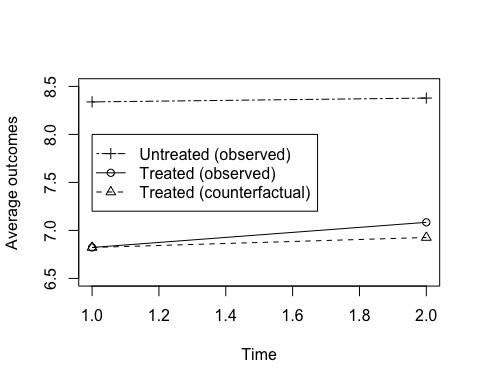
\includegraphics[width=0.6\linewidth]{STCI_files/figure-latex/ploty0y1yBD-1} 

}

\caption{Evolution of average outcomes in the treated and control group before (Time =1) and after (Time=2) the treatment}\label{fig:ploty0y1yBD}
\end{figure}

The estimate of the \(WW\) comparison in the sample is thus:

\begin{align*}
\hat{\Delta^Y_{WW}} & = \frac{1}{\sum_{i=1}^N D_i}\sum_{i=1}^N Y_iD_i-\frac{1}{\sum_{i=1}^N (1-D_i)}\sum_{i=1}^N Y_i(1-D_i).
\end{align*}

We have \(\hat{\Delta^y_{WW}}=\) -1.308.
Remember that the value of \(TT\) in the sample is \(\Delta^y_{TT_s}=\) 0.168.

Overall, \(WW\) severely underestimates the effect of the treatment in our example.
\(WW\) suggests that the treatment has a negative effect on outcomes whereas we know by construction that it has a positive one.

\hypertarget{selection-bias}{%
\subsubsection{Selection bias}\label{selection-bias}}

When we form the with/without comparison, we do not recover the \(TT\) parameter.
Instead, we recover \(TT\) plus a bias term, called \textbf{selection bias}:

\begin{align*}
\Delta^Y_{WW} & =\Delta^Y_{TT}+\Delta^Y_{SB}.
\end{align*}

\BeginKnitrBlock{definition}[Selection bias]
\protect\hypertarget{def:SB}{}{\label{def:SB} \iffalse (Selection bias) \fi{} }Selection bias is the difference between the with/without comparison and the treatment on the treated parameter:
\begin{align*}
\Delta^Y_{SB} & = \Delta^Y_{WW}-\Delta^Y_{TT}.
\end{align*}
\EndKnitrBlock{definition}

\(WW\) tries to approximate the counterfactual expected outcome in the treated group by using \(\esp{Y_i^0|D_i=0}\), the expected outcome in the untreated group .
Selection bias appears because this proxy is generally poor.
It is very easy to see that selection bias is indeed directly due to this bad proxy problem:

\BeginKnitrBlock{theorem}[Selection bias and counterfactual]
\protect\hypertarget{thm:SBth}{}{\label{thm:SBth} \iffalse (Selection bias and counterfactual) \fi{} }Selection bias is the difference between the counterfactual expected potential outcome in the absence of the treatment among the treated and the expected potential outcome in the absence of the treatment among the untreated.

\begin{align*}
\Delta^Y_{SB} & = \esp{Y_i^0|D_i=1}-\esp{Y_i^0|D_i=0}.
\end{align*}
\EndKnitrBlock{theorem}

\BeginKnitrBlock{proof}
\iffalse{} {Proof. } \fi{}\begin{align*}
\Delta^Y_{SB} & = \Delta^Y_{WW}-\Delta^Y_{TT} \\
              & = \esp{Y_i|D_i=1}-\esp{Y_i|D_i=0}-\esp{Y_i^1-Y_i^0|D_i=1}\\
              & = \esp{Y_i^0|D_i=1}-\esp{Y_i^0|D_i=0}.
\end{align*}

The first and second equalities stem only from the definition of both parameters.
The third equality stems from using the switching equation: \(Y_i=Y_i^1D_i+Y_i^0(1-D_i)\), so that \(\esp{Y_i|D_i=1}=\esp{Y^1_i|D_i=1}\) and \(\esp{Y_i|D_i=0}=\esp{Y_i^0|D_i=0}\).
\EndKnitrBlock{proof}

\BeginKnitrBlock{example}
\protect\hypertarget{exm:unnamed-chunk-17}{}{\label{exm:unnamed-chunk-17} }In the population, \(SB\) is equal to
\EndKnitrBlock{example}

\begin{align*}
  \Delta^y_{SB} & = \Delta^y_{WW}-\Delta^y_{TT} \\
                & = -1.298 - 0.172 \\
                & = -1.471
\end{align*}

We could have computed \(SB\) directly using the formula from Theorem \ref{thm:SBth}:

\begin{align*}
\Delta^y_{SB} & = \esp{y_i^0|D_i=1}-\esp{y_i^0|D_i=0}\\
              & = -\frac{\sigma^2_{\mu}+\rho\sigma^2_{U}}{\sqrt{\sigma^2_{\mu}+\sigma^2_{U}}}\left(\frac{\phi\left(\frac{\bar{y}-\bar{\mu}}{\sqrt{\sigma^2_{\mu}+\sigma^2_{U}}}\right)}{\Phi\left(\frac{\bar{y}-\bar{\mu}}{\sqrt{\sigma^2_{\mu}+\sigma^2_{U}}}\right)}+\frac{\phi\left(\frac{\bar{y}-\bar{\mu}}{\sqrt{\sigma^2_{\mu}+\sigma^2_{U}}}\right)}{1-\Phi\left(\frac{\bar{y}-\bar{\mu}}{\sqrt{\sigma^2_{\mu}+\sigma^2_{U}}}\right)}\right).
\end{align*}

When using the R function for \(SB\) that we have defined earlier, we indeed find: \(\Delta^y_{SB}=\) -1.471.

In the sample, \(\hat{\Delta^y_{SB}}=\)-1.308-0.168 \(=\) -1.476.
Selection bias emerges because we are using a bad proxy for the counterfactual.
The average outcome for the untreated is equal to \(\frac{1}{\sum_{i=1}^N(1-D_i)}\sum_{i=1}^N(1-D_i)y_i=\) 8.383 while the counterfactual average outcome for the treated is \(\frac{1}{\sum_{i=1}^ND_i}\sum_{i=1}^ND_iy^0_i=\) 6.906.
Their difference is as expected equal to \(SB\):
\(\hat{\Delta^y_{SB}}=\) 6.906 \(-\) 8.383 \(=\) -1.476.
The counterfactual average outcome of the treated is much smaller than the average outcome of the untreated.
On Figure \ref{fig:ploty0y1yBD}, this is materialized by the fact that the plus sign is located much above the triangle.

\BeginKnitrBlock{remark}
\iffalse{} {Remark. } \fi{}The concept of selection bias is related to but different from the concept of sample selection bias.
With sample selection bias, we worry that selection into the sample might bias the estimated effect of a treatment on outcomes.
With selection bias, we worry that selection into the treatment itself might bias the effect of the treatment on outcomes.
Both biases are due to unbserved covariates, but they do not play out in the same way.

For example, estimating the effect of education on women's wages raises both selection bias and sample selection bias issues.
Selection bias stems from the fact that more educated women are more likely to be more dynamic and thus to have higher earnings even when less educated.
Selection bias would be positive in that case, overestimating the effect of education on earnings.

Sample selection bias stems from the fact that we can only use a sample of working women in order to estimate the effect of education on wages, since we do not observe the wages on non working women.
But, selection into the labor force might generate sample selection bias.
More educated women participate more in the labor market, while less educated women participate less.
As a consequence, less educated women that work are different from the overall sample of less educated women.
They might be more dynamic and work-focused.
As a consequence, their wages are higher than the average wages of the less educated women.
Comparing the wages of less educated women that work to those of more educated women that work might understate the effect of education on earnings.
Sample selection bias would generate a negative bias on the education coefficient.
\EndKnitrBlock{remark}

\hypertarget{confounding-factors}{%
\subsubsection{Confounding factors}\label{confounding-factors}}

Confounding factors are the factors that generate differences between treated and untreated individuals even in the absence of the treatment.
The confounding factors are thus responsible for selection bias.
In general, the mere fact of being selected for receiving the treatment means that you have a host of characteristics that would differentiate you from the unselected individuals, even if you were not to receive the treatment eventually.

For example, if a drug is given to initially sicker individuals, then, we expect that they will be sicker that the untreated in the absence of the treatment.
Comparing sick individuals to healthy ones is not a sound way to estimate the effect of a treatment.
Obviously, even if our treatment performs well, healthier individuals will be healthier after the treatment has been allocated to the sicker patients.
The best we can expect is that the treated patients have recovered, and that their health after the treatment is comparable to that of the untreated patients.
In that case, the with/without comparison is going to be null, whereas the true effect of the treatment is positive.
Selection bias is negative in that case: in the absence of the treatment, the average health status of the treated individuals would have been smaller than that of the untreated individuals.
The confounding factor is the health status of individuals when the decision to allocate the drug has been taken.
It is correlated to both the allocation of the treatment (negatively) and to health in the absence of the treatment (positively).

\BeginKnitrBlock{example}
\protect\hypertarget{exm:unnamed-chunk-19}{}{\label{exm:unnamed-chunk-19} }In our example, \(\mu_i\) and \(U_i^B\) are the confounding factors.
Because the treatment is only given to individuals with pre-treament outcomes smaller than a threshold (\(y_i^B\leq\bar{y}\)), participants tend to have smaller \(\mu_i\) and \(U_i^B\) than non participants, as we can see on Figure \ref{fig:histmuD}.
\EndKnitrBlock{example}

\begin{figure}[htbp]

{\centering 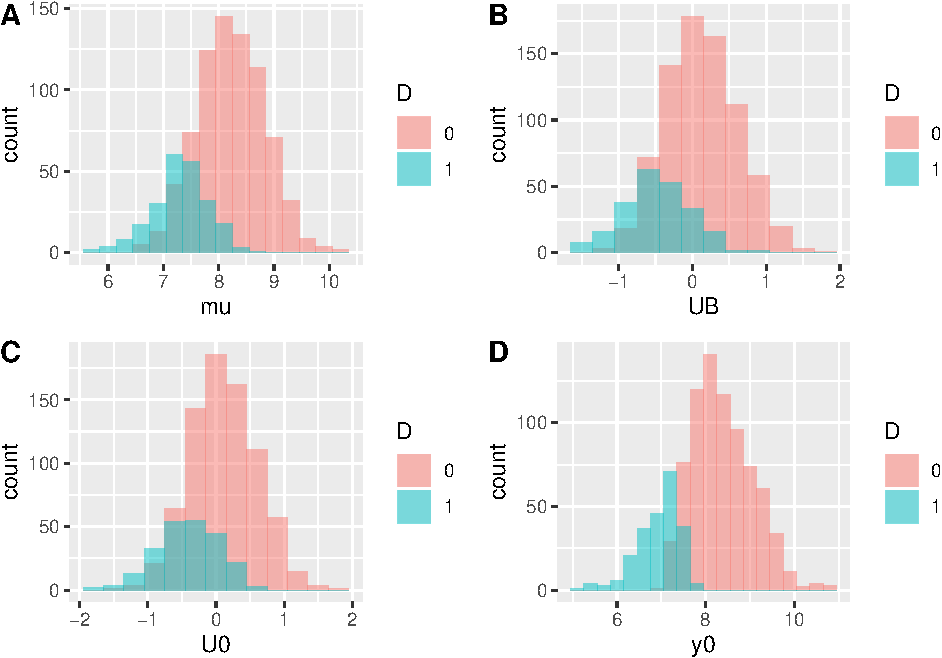
\includegraphics[width=0.6\linewidth]{STCI_files/figure-latex/histmuD-1} 

}

\caption{Distribution of confounders in the treated and control group}\label{fig:histmuD}
\end{figure}

Since confounding factors are persistent, they affect the outcomes of participants and non participants after the treatment date.
\(\mu_i\) persists entirely over time, and \(U_i^B\) persists at a rate \(\rho\).
As a consequence, even in the absence of the treatment, participants have lower outcomes than non participants, as we can see on Figure \ref{fig:histmuD}.

We can derive the contributions of both confouding factors to overall SB:

\begin{align*}
\esp{Y_i^0|D_i=1} & = \esp{\mu_i+\delta+U_i^0|\mu_i+U_i^B\leq\bar{y}}\\
                  & = \delta + \esp{\mu_i|\mu_i+U_i^B\leq\bar{y}} + \rho\esp{U_i^B|\mu_i+U_i^B\leq\bar{y}}\\
\Delta^y_{SB}     & = \esp{\mu_i|\mu_i+U_i^B\leq\bar{y}}-\esp{\mu_i|\mu_i+U_i^B>\bar{y}} \\
                  & \phantom{=} + \rho\left(\esp{U_i^B|\mu_i+U_i^B\leq\bar{y}}-\esp{U_i^B|\mu_i+U_i^B>\bar{y}}\right)\\
                  & = -\frac{\sigma^2_{\mu}}{\sqrt{\sigma^2_{\mu}+\sigma^2_{U}}}\left(\frac{\phi\left(\frac{\bar{y}-\bar{\mu}}{\sqrt{\sigma^2_{\mu}+\sigma^2_{U}}}\right)}{\Phi\left(\frac{\bar{y}-\bar{\mu}}{\sqrt{\sigma^2_{\mu}+\sigma^2_{U}}}\right)}+\frac{\phi\left(\frac{\bar{y}-\bar{\mu}}{\sqrt{\sigma^2_{\mu}+\sigma^2_{U}}}\right)}{1-\Phi\left(\frac{\bar{y}-\bar{\mu}}{\sqrt{\sigma^2_{\mu}+\sigma^2_{U}}}\right)}\right) \\
                  & \phantom{=} -\frac{\rho\sigma^2_{U}}{\sqrt{\sigma^2_{\mu}+\sigma^2_{U}}}\left(\frac{\phi\left(\frac{\bar{y}-\bar{\mu}}{\sqrt{\sigma^2_{\mu}+\sigma^2_{U}}}\right)}{\Phi\left(\frac{\bar{y}-\bar{\mu}}{\sqrt{\sigma^2_{\mu}+\sigma^2_{U}}}\right)}+\frac{\phi\left(\frac{\bar{y}-\bar{\mu}}{\sqrt{\sigma^2_{\mu}+\sigma^2_{U}}}\right)}{1-\Phi\left(\frac{\bar{y}-\bar{\mu}}{\sqrt{\sigma^2_{\mu}+\sigma^2_{U}}}\right)}\right)
\end{align*}

In order to evaluate these quantities, let's build two R functions:

\begin{Shaded}
\begin{Highlighting}[]
\NormalTok{delta.y.sb.mu <-}\StringTok{ }\ControlFlowTok{function}\NormalTok{(param)\{}
  \KeywordTok{return}\NormalTok{(}\OperatorTok{-}\NormalTok{(param[}\StringTok{"sigma2mu"}\NormalTok{])}\OperatorTok{/}\KeywordTok{sqrt}\NormalTok{(param[}\StringTok{"sigma2mu"}\NormalTok{]}\OperatorTok{+}\NormalTok{param[}\StringTok{"sigma2U"}\NormalTok{])}
         \OperatorTok{*}\KeywordTok{dnorm}\NormalTok{((}\KeywordTok{log}\NormalTok{(param[}\StringTok{"barY"}\NormalTok{])}\OperatorTok{-}\NormalTok{param[}\StringTok{"barmu"}\NormalTok{])}\OperatorTok{/}\NormalTok{(}\KeywordTok{sqrt}\NormalTok{(param[}\StringTok{"sigma2mu"}\NormalTok{]}\OperatorTok{+}\NormalTok{param[}\StringTok{"sigma2U"}\NormalTok{])))}
         \OperatorTok{*}\NormalTok{(}\DecValTok{1}\OperatorTok{/}\KeywordTok{pnorm}\NormalTok{((}\KeywordTok{log}\NormalTok{(param[}\StringTok{"barY"}\NormalTok{])}\OperatorTok{-}\NormalTok{param[}\StringTok{"barmu"}\NormalTok{])}\OperatorTok{/}\NormalTok{(}\KeywordTok{sqrt}\NormalTok{(param[}\StringTok{"sigma2mu"}\NormalTok{]}\OperatorTok{+}\NormalTok{param[}\StringTok{"sigma2U"}\NormalTok{])))}
           \OperatorTok{+}\DecValTok{1}\OperatorTok{/}\NormalTok{(}\DecValTok{1}\OperatorTok{-}\KeywordTok{pnorm}\NormalTok{((}\KeywordTok{log}\NormalTok{(param[}\StringTok{"barY"}\NormalTok{])}\OperatorTok{-}\NormalTok{param[}\StringTok{"barmu"}\NormalTok{])}\OperatorTok{/}\NormalTok{(}\KeywordTok{sqrt}\NormalTok{(param[}\StringTok{"sigma2mu"}\NormalTok{]}\OperatorTok{+}\NormalTok{param[}\StringTok{"sigma2U"}\NormalTok{]))))))}
\NormalTok{\}}
\NormalTok{delta.y.sb.U <-}\StringTok{ }\ControlFlowTok{function}\NormalTok{(param)\{}
  \KeywordTok{return}\NormalTok{(}\OperatorTok{-}\NormalTok{(param[}\StringTok{"rho"}\NormalTok{]}\OperatorTok{*}\NormalTok{param[}\StringTok{"sigma2U"}\NormalTok{])}\OperatorTok{/}\KeywordTok{sqrt}\NormalTok{(param[}\StringTok{"sigma2mu"}\NormalTok{]}\OperatorTok{+}\NormalTok{param[}\StringTok{"sigma2U"}\NormalTok{])}
         \OperatorTok{*}\KeywordTok{dnorm}\NormalTok{((}\KeywordTok{log}\NormalTok{(param[}\StringTok{"barY"}\NormalTok{])}\OperatorTok{-}\NormalTok{param[}\StringTok{"barmu"}\NormalTok{])}\OperatorTok{/}\NormalTok{(}\KeywordTok{sqrt}\NormalTok{(param[}\StringTok{"sigma2mu"}\NormalTok{]}\OperatorTok{+}\NormalTok{param[}\StringTok{"sigma2U"}\NormalTok{])))}
         \OperatorTok{*}\NormalTok{(}\DecValTok{1}\OperatorTok{/}\KeywordTok{pnorm}\NormalTok{((}\KeywordTok{log}\NormalTok{(param[}\StringTok{"barY"}\NormalTok{])}\OperatorTok{-}\NormalTok{param[}\StringTok{"barmu"}\NormalTok{])}\OperatorTok{/}\NormalTok{(}\KeywordTok{sqrt}\NormalTok{(param[}\StringTok{"sigma2mu"}\NormalTok{]}\OperatorTok{+}\NormalTok{param[}\StringTok{"sigma2U"}\NormalTok{])))}
           \OperatorTok{+}\DecValTok{1}\OperatorTok{/}\NormalTok{(}\DecValTok{1}\OperatorTok{-}\KeywordTok{pnorm}\NormalTok{((}\KeywordTok{log}\NormalTok{(param[}\StringTok{"barY"}\NormalTok{])}\OperatorTok{-}\NormalTok{param[}\StringTok{"barmu"}\NormalTok{])}\OperatorTok{/}\NormalTok{(}\KeywordTok{sqrt}\NormalTok{(param[}\StringTok{"sigma2mu"}\NormalTok{]}\OperatorTok{+}\NormalTok{param[}\StringTok{"sigma2U"}\NormalTok{]))))))}
\NormalTok{\}}
\end{Highlighting}
\end{Shaded}

The contribution of \(\mu_i\) to selection bias is -0.978 while that of \(U_i^0\) is of -0.493.

\hypertarget{when-does-ww-identify-tt}{%
\subsubsection{\texorpdfstring{When does \(WW\) identify \(TT\)?}{When does WW identify TT?}}\label{when-does-ww-identify-tt}}

Are there conditions under which \(WW\) identify \(TT\)?
The answer is yes: when there is no selection bias, the proxy used by \(WW\) for the counterfactual quantity is actually valid.
Formally, \(WW\) identifies \(TT\) when the following assumption holds:

\BeginKnitrBlock{definition}[No selection bias]
\protect\hypertarget{def:noselb}{}{\label{def:noselb} \iffalse (No selection bias) \fi{} }We assume the following:
\begin{align*}
\esp{Y_i^0|D_i=1} & = \esp{Y_i^0|D_i=0}.
\end{align*}
\EndKnitrBlock{definition}

Under Assumption \ref{def:noselb}, the expected counterfactual outcome of the treated is equal to the expected potential outcome of the untreated in the absence of the treatment.
This yields to the following result:

\BeginKnitrBlock{theorem}
\protect\hypertarget{thm:wwtt}{}{\label{thm:wwtt} }Under Assumption \ref{def:noselb}, \(WW\) identifies the \(TT\) parameter:
\begin{align*}
\Delta^Y_{WW} & = \Delta^Y_{TT}.
\end{align*}
\EndKnitrBlock{theorem}

\BeginKnitrBlock{proof}
\iffalse{} {Proof. } \fi{}\begin{align*}
\Delta^Y_{WW} & = \esp{Y_i|D_i=1}-\esp{Y_i|D_i=0}\\
              & = \esp{Y_i^1|D_i=1}-\esp{Y_i^0|D_i=0}\\
              & = \esp{Y_i^1|D_i=1}-\esp{Y_i^0|D_i=1} \\
              & = \Delta^Y_{TT},
\end{align*}
where the second equation uses the switching equation and the third uses Assumption \ref{def:noselb}.
\EndKnitrBlock{proof}

So, under Assumption \ref{def:noselb}, the \(WW\) comparison actually identifies the \(TT\) parameter.
We say that Assumption \ref{def:noselb} is an \textbf{identification assumption}: it serves to identify the parameter of interest using observed data.
The intuition for this result is simply that, under Assumption \ref{def:noselb}, there are no confounding factors and thus no selection bias.
under Assumption \ref{def:noselb}, the factors that yield individuals to receive or not the treatment are mean-independent of the potential outcomes in the absence of the treatment.
In this case, the expected outcome in the untreated group actually is a perfect proxy for the counterfactual expected outcome of the treated group.

Obviously, Assumption \ref{def:noselb} is extremely unlikely to hold in real life.
For Assumption \ref{def:noselb} to hold, it has to be that \textbf{all} the determinants of \(D_i\) are actually unrelated to \(Y_i^0\).
One way to enforce Assumption \ref{def:noselb} is to randomize treatment intake.
We will see this in the Lecture on RCTs.
It might also be possible that Assumption \ref{def:noselb} holds in the data in the absence of an RCT.
But this is not very likely, and should be checked by every mean possible.

One way to test for the validity of Assumption \ref{def:noselb} is to compare the values of observed covariates in the treated and untreated group.
For Assumption \ref{def:noselb} to be credible, observed covariates should be distributed in the same way.

Another nice way to test for the validity of Assumption \ref{def:noselb} with observed data is to implement a \textbf{placebo test}.
A placebo test looks for an effect where there should be none, if we believe the identification assumptions.
For example, under Assumption \ref{def:noselb} it should be (even though it is not rigorously implied) that outcomes before the treatment are also mean-independent of the treatment allocation.
And actually, since a future treatment cannot have an effect today (unless people anticipate the treatment, which we assume away here), the \(WW\) comparison before the treatment should be null, therefore giving a zero effect of the placebo treatment ``will receive the treatment in the future.''

\BeginKnitrBlock{example}
\protect\hypertarget{exm:unnamed-chunk-21}{}{\label{exm:unnamed-chunk-21} }When the allocation rule defining \(D_i\) is the eligibility rule that we have used so far, we have already seen that Assumption \ref{def:noselb} does not hold and the placebo test should not pass either.
\EndKnitrBlock{example}

One way of generating Assumption \ref{def:noselb} from the eligibility rule that we are using is to mute the persistence in outcome dynamics.
For example, one could set \(\rho=0\) and \(\sigma^2_{\mu}=0\).

\begin{Shaded}
\begin{Highlighting}[]
\NormalTok{param <-}\StringTok{ }\KeywordTok{c}\NormalTok{(}\DecValTok{8}\NormalTok{,}\DecValTok{0}\NormalTok{,.}\DecValTok{28}\NormalTok{,}\DecValTok{1500}\NormalTok{,}\DecValTok{0}\NormalTok{,}\FloatTok{0.01}\NormalTok{,}\FloatTok{0.05}\NormalTok{,}\FloatTok{0.05}\NormalTok{,}\FloatTok{0.05}\NormalTok{,}\FloatTok{0.1}\NormalTok{)}
\KeywordTok{names}\NormalTok{(param) <-}\StringTok{ }\KeywordTok{c}\NormalTok{(}\StringTok{"barmu"}\NormalTok{,}\StringTok{"sigma2mu"}\NormalTok{,}\StringTok{"sigma2U"}\NormalTok{,}\StringTok{"barY"}\NormalTok{,}\StringTok{"rho"}\NormalTok{,}\StringTok{"theta"}\NormalTok{,}\StringTok{"sigma2epsilon"}\NormalTok{,}\StringTok{"sigma2eta"}\NormalTok{,}\StringTok{"delta"}\NormalTok{,}\StringTok{"baralpha"}\NormalTok{)}
\NormalTok{param}
\end{Highlighting}
\end{Shaded}

\begin{verbatim}
##         barmu      sigma2mu       sigma2U          barY           rho 
##          8.00          0.00          0.28       1500.00          0.00 
##         theta sigma2epsilon     sigma2eta         delta      baralpha 
##          0.01          0.05          0.05          0.05          0.10
\end{verbatim}

In that case, outcomes are not persistent and Assumption \ref{def:noselb} holds:

\begin{align*}
\esp{y_i^0|D_i=1} & = \esp{\mu_i+\delta+U_i^0|y_i^B\leq\bar{y}}\\
                  & = \esp{\bar{\mu}+\delta+\epsilon_i|\bar{\mu}+U_i^B\leq\bar{y}}\\
                  & = \bar{\mu} + \delta + \esp{\epsilon_i|\bar{\mu}+U_i^B\leq\bar{y}}\\
                  & = \bar{\mu} + \delta + \esp{\epsilon_i|\bar{\mu}+U_i^B>\bar{y}}\\
                  & = \esp{\mu_i+\delta+U_i^0|y_i^B>\bar{y}}\\
                  & = \esp{y_i^0|D_i=0},                  
\end{align*}

where the second equality follows from \(\sigma^2_{\mu}=0\) and \(\rho=0\) and the fourth from \(\epsilon_i \Ind U_i^B\).
Another direct way to see this is to use the formula for selection bias that we have derived above.
It is easy to see that with \(\rho=0\) and \(\sigma^2_{\mu}=0\), \(\Delta^y_{SB}=0\).
To be sure, we can compute \(\Delta^y_{SB}\) with the new parameter values: \(\Delta^y_{SB}=\) 0.
As a consequence, \(\Delta^y_{TT}=\) 0.18 \(=\) 0.18 \(=\Delta^y_{WW}\).

\BeginKnitrBlock{remark}
\iffalse{} {Remark. } \fi{}You might have noticed that the value of \(\Delta^y_{TT}\) is different than before.
It is normal, since it depends on the values of parameters, and especially on \(\sigma_{\mu}^2\) and \(\rho\).
\EndKnitrBlock{remark}

Let's see how these quantities behave in the sample.

\begin{Shaded}
\begin{Highlighting}[]
\KeywordTok{set.seed}\NormalTok{(}\DecValTok{1234}\NormalTok{)}
\NormalTok{mu <-}\StringTok{ }\KeywordTok{rnorm}\NormalTok{(N,param[}\StringTok{"barmu"}\NormalTok{],}\KeywordTok{sqrt}\NormalTok{(param[}\StringTok{"sigma2mu"}\NormalTok{]))}
\NormalTok{UB <-}\StringTok{ }\KeywordTok{rnorm}\NormalTok{(N,}\DecValTok{0}\NormalTok{,}\KeywordTok{sqrt}\NormalTok{(param[}\StringTok{"sigma2U"}\NormalTok{]))}
\NormalTok{yB <-}\StringTok{ }\NormalTok{mu }\OperatorTok{+}\StringTok{ }\NormalTok{UB }
\NormalTok{YB <-}\StringTok{ }\KeywordTok{exp}\NormalTok{(yB)}
\NormalTok{Ds <-}\StringTok{ }\KeywordTok{rep}\NormalTok{(}\DecValTok{0}\NormalTok{,N)}
\NormalTok{Ds[YB}\OperatorTok{<=}\NormalTok{param[}\StringTok{"barY"}\NormalTok{]] <-}\StringTok{ }\DecValTok{1} 
\NormalTok{epsilon <-}\StringTok{ }\KeywordTok{rnorm}\NormalTok{(N,}\DecValTok{0}\NormalTok{,}\KeywordTok{sqrt}\NormalTok{(param[}\StringTok{"sigma2epsilon"}\NormalTok{]))}
\NormalTok{eta<-}\StringTok{ }\KeywordTok{rnorm}\NormalTok{(N,}\DecValTok{0}\NormalTok{,}\KeywordTok{sqrt}\NormalTok{(param[}\StringTok{"sigma2eta"}\NormalTok{]))}
\NormalTok{U0 <-}\StringTok{ }\NormalTok{param[}\StringTok{"rho"}\NormalTok{]}\OperatorTok{*}\NormalTok{UB }\OperatorTok{+}\StringTok{ }\NormalTok{epsilon}
\NormalTok{y0 <-}\StringTok{ }\NormalTok{mu }\OperatorTok{+}\StringTok{  }\NormalTok{U0 }\OperatorTok{+}\StringTok{ }\NormalTok{param[}\StringTok{"delta"}\NormalTok{]}
\NormalTok{alpha <-}\StringTok{ }\NormalTok{param[}\StringTok{"baralpha"}\NormalTok{]}\OperatorTok{+}\StringTok{  }\NormalTok{param[}\StringTok{"theta"}\NormalTok{]}\OperatorTok{*}\NormalTok{mu }\OperatorTok{+}\StringTok{ }\NormalTok{eta}
\NormalTok{y1 <-}\StringTok{ }\NormalTok{y0}\OperatorTok{+}\NormalTok{alpha}
\NormalTok{Y0 <-}\StringTok{ }\KeywordTok{exp}\NormalTok{(y0)}
\NormalTok{Y1 <-}\StringTok{ }\KeywordTok{exp}\NormalTok{(y1)}
\NormalTok{y <-}\StringTok{ }\NormalTok{y1}\OperatorTok{*}\NormalTok{Ds}\OperatorTok{+}\NormalTok{y0}\OperatorTok{*}\NormalTok{(}\DecValTok{1}\OperatorTok{-}\NormalTok{Ds)}
\NormalTok{Y <-}\StringTok{ }\NormalTok{Y1}\OperatorTok{*}\NormalTok{Ds}\OperatorTok{+}\NormalTok{Y0}\OperatorTok{*}\NormalTok{(}\DecValTok{1}\OperatorTok{-}\NormalTok{Ds)}
\end{Highlighting}
\end{Shaded}

We can see that \(\hat{\esp{Y_i^0|D_i=1}}=\) 8.038 \(\approx\) 8.055 \(=\hat{\esp{Y_i^0|D_i=0}}\).
This means that \(WW\) should be close to \(TT\): \(\hat{\Delta^y_{TT}}=\) 0.198 \(\approx\) 0.182 \(=\hat{\Delta^y_{WW}}\).
Note that \(\hat{WW}\) in the sample is not exactly, but only approximately, equal to \(TT\) in the population and in the sample.
This is an instance of the Fundamental Problem of Statistical Inference that we will study in the next chapter.

Under these restrictions, the placebo test would unfortunately conclude against Assumption \ref{def:noselb} even though it is valid:

\begin{align*}
\esp{y_i^B|D_i=1} & = \esp{\mu_i+ U_i^B|y_i^B\leq\bar{y}}\\
                  & = \esp{\bar{\mu}+U_i^B|\bar{\mu}+U_i^B\leq\bar{y}}\\
                  & = \bar{\mu}  + \esp{U_i^B|\bar{\mu}+U_i^B\leq\bar{y}}\\
                  & \neq \bar{\mu}  + \esp{U_i^B|\bar{\mu}+U_i^B>\bar{y}}\\
                  & = \esp{\mu_i+U_i^0|y_i^B>\bar{y}}\\
                  & = \esp{y_i^B|D_i=0}.                  
\end{align*}

In the sample, we indeed have that \(\hat{\esp{Y_i^B|D_i=1}}=\) 7.004 \(\neq\) 8.072 \(=\hat{\esp{Y_i^B|D_i=0}}\).
The reason for the failure of the placebo test to conclude that \(Ww\) is actually correct is that the \(U_i^B\) shock enters both into the selection equation and the outcome equation for \(y_i^B\), generating a wage at period \(B\) between the outcomes of the treated and of the untreated.
Since it is not persistent, this wedge does not generate selection bias.
This wedge would not be detected if we could perform it further back in time, before the selection period.

Another way to make Assumption \ref{def:noselb} work is to generate a new allocation rule where all the determinants of treatment intake are indeed orthogonal to potential outcomes and to outcomes before the treatment.
Let's assume for example that \(D_i=\uns{V_i\leq\bar{y}}\), with \(V_i\sim\mathcal{N}(\bar{\mu},\sigma^2_{\mu}+\sigma^2_{U})\) and \(V_i\Ind(Y_i^0,Y_i^1,Y_i^B,\mu_i,\eta_i)\).
In that case, Assumption \ref{def:noselb} holds and the placebo test does work.
Indeed, we have:

\begin{align*}
\Delta^y_{TT} & = \esp{Y_i^1-Y_i^0|D_i=1} \\
              & = \esp{\alpha_i|D_i=1} \\
              & = \esp{\bar{\alpha}+\theta\mu_i+\eta_i|V_i\leq\bar{y}}\\
              & = \bar{\alpha}+\theta\bar{\mu} \\
              & = \Delta^y_{ATE} \\
\Delta^y_{WW} & = \esp{Y_i|D_i=1} - \esp{Y_i|D_i=0} \\
              & = \esp{Y^1_i|D_i=1} - \esp{Y^0_i|D_i=0} \\
              & = \esp{Y^1_i|V_i\leq\bar{y}} - \esp{Y^0_i|V_i>\bar{y}} \\
              & = \esp{Y^1_i} - \esp{Y^0_i} \\
              & = \Delta^y_{ATE}
\end{align*}

\(ATE\) is the Average Treatment Effect in the population.
It is the expected effect of the treatment on all the members of the population, not only on the treated.
When the treatment is randomly allocated, both \(TT\) and \(ATE\) are equal, since the treated are a random subset of the overall population.
I prefer to use \(ATE\) for my definition of the \(R\) function in order not to erase the definition of the \(TT\) function:

\begin{Shaded}
\begin{Highlighting}[]
\NormalTok{delta.y.ate <-}\StringTok{ }\ControlFlowTok{function}\NormalTok{(param)\{}
  \KeywordTok{return}\NormalTok{(param[}\StringTok{"baralpha"}\NormalTok{]}\OperatorTok{+}\NormalTok{param[}\StringTok{"theta"}\NormalTok{]}\OperatorTok{*}\NormalTok{param[}\StringTok{"barmu"}\NormalTok{])}
\NormalTok{\}}
\end{Highlighting}
\end{Shaded}

In the population, \(WW\) identifies \(TT\): \(\Delta^y_{TT}=\) 0.18 \(=\Delta^y_{WW}\).
Let's see how these quantities behave in the sample:

\begin{Shaded}
\begin{Highlighting}[]
\KeywordTok{set.seed}\NormalTok{(}\DecValTok{1234}\NormalTok{)}
\NormalTok{N <-}\DecValTok{1000}
\NormalTok{mu <-}\StringTok{ }\KeywordTok{rnorm}\NormalTok{(N,param[}\StringTok{"barmu"}\NormalTok{],}\KeywordTok{sqrt}\NormalTok{(param[}\StringTok{"sigma2mu"}\NormalTok{]))}
\NormalTok{UB <-}\StringTok{ }\KeywordTok{rnorm}\NormalTok{(N,}\DecValTok{0}\NormalTok{,}\KeywordTok{sqrt}\NormalTok{(param[}\StringTok{"sigma2U"}\NormalTok{]))}
\NormalTok{yB <-}\StringTok{ }\NormalTok{mu }\OperatorTok{+}\StringTok{ }\NormalTok{UB }
\NormalTok{YB <-}\StringTok{ }\KeywordTok{exp}\NormalTok{(yB)}
\NormalTok{Ds <-}\StringTok{ }\KeywordTok{rep}\NormalTok{(}\DecValTok{0}\NormalTok{,N)}
\NormalTok{V <-}\StringTok{ }\KeywordTok{rnorm}\NormalTok{(N,param[}\StringTok{"barmu"}\NormalTok{],}\KeywordTok{sqrt}\NormalTok{(param[}\StringTok{"sigma2mu"}\NormalTok{]}\OperatorTok{+}\NormalTok{param[}\StringTok{"sigma2U"}\NormalTok{]))}
\NormalTok{Ds[V}\OperatorTok{<=}\KeywordTok{log}\NormalTok{(param[}\StringTok{"barY"}\NormalTok{])] <-}\StringTok{ }\DecValTok{1} 
\NormalTok{epsilon <-}\StringTok{ }\KeywordTok{rnorm}\NormalTok{(N,}\DecValTok{0}\NormalTok{,}\KeywordTok{sqrt}\NormalTok{(param[}\StringTok{"sigma2epsilon"}\NormalTok{]))}
\NormalTok{eta<-}\StringTok{ }\KeywordTok{rnorm}\NormalTok{(N,}\DecValTok{0}\NormalTok{,}\KeywordTok{sqrt}\NormalTok{(param[}\StringTok{"sigma2eta"}\NormalTok{]))}
\NormalTok{U0 <-}\StringTok{ }\NormalTok{param[}\StringTok{"rho"}\NormalTok{]}\OperatorTok{*}\NormalTok{UB }\OperatorTok{+}\StringTok{ }\NormalTok{epsilon}
\NormalTok{y0 <-}\StringTok{ }\NormalTok{mu }\OperatorTok{+}\StringTok{  }\NormalTok{U0 }\OperatorTok{+}\StringTok{ }\NormalTok{param[}\StringTok{"delta"}\NormalTok{]}
\NormalTok{alpha <-}\StringTok{ }\NormalTok{param[}\StringTok{"baralpha"}\NormalTok{]}\OperatorTok{+}\StringTok{  }\NormalTok{param[}\StringTok{"theta"}\NormalTok{]}\OperatorTok{*}\NormalTok{mu }\OperatorTok{+}\StringTok{ }\NormalTok{eta}
\NormalTok{y1 <-}\StringTok{ }\NormalTok{y0}\OperatorTok{+}\NormalTok{alpha}
\NormalTok{Y0 <-}\StringTok{ }\KeywordTok{exp}\NormalTok{(y0)}
\NormalTok{Y1 <-}\StringTok{ }\KeywordTok{exp}\NormalTok{(y1)}
\NormalTok{y <-}\StringTok{ }\NormalTok{y1}\OperatorTok{*}\NormalTok{Ds}\OperatorTok{+}\NormalTok{y0}\OperatorTok{*}\NormalTok{(}\DecValTok{1}\OperatorTok{-}\NormalTok{Ds)}
\NormalTok{Y <-}\StringTok{ }\NormalTok{Y1}\OperatorTok{*}\NormalTok{Ds}\OperatorTok{+}\NormalTok{Y0}\OperatorTok{*}\NormalTok{(}\DecValTok{1}\OperatorTok{-}\NormalTok{Ds)}
\end{Highlighting}
\end{Shaded}

In the sample, the counterfactual is well approximated by the outcomes of the untreated: \(\hat{\esp{Y_i^0|D_i=1}}=\) 8.085 \(\approx\) 8.054 \(=\hat{\esp{Y_i^0|D_i=0}}\).
As a consequence, \(WW\) should be close to \(TT\): \(\hat{\Delta^y_{TT}}=\) 0.168 \(\approx\) 0.199 \(=\hat{\Delta^y_{WW}}\).
The placebo test is also valid in that case: \(\hat{\esp{Y_i^B|D_i=1}}=\) 7.95 \(\approx\) 7.99 \(=\hat{\esp{Y_i^B|D_i=0}}\).

\hypertarget{the-beforeafter-comparison-temporal-confounders-and-time-trend-bias}{%
\subsection{The before/after comparison, temporal confounders and time trend bias}\label{the-beforeafter-comparison-temporal-confounders-and-time-trend-bias}}

The before/after comparison (\(BA\)) is also very intuitive: it consists in looking at how the outcomes of the treated have changed over time and to attribute this change to the effect of the treatment.
The problem is that other changes might have affected outcomes in the absence of the treatment, thereby biasing \(BA\).
The bias of \(BA\) is called time-trend bias.
It is due to confounders that affect the outcomes of the treated over time.
This section defines the \(BA\) estimator, derives its bias, describes the role of the confounders and states conditions under which \(BA\) identifies \(TT\).

\BeginKnitrBlock{example}
\protect\hypertarget{exm:unnamed-chunk-23}{}{\label{exm:unnamed-chunk-23} }Before computing any estimates, we need to reset all our parameter values and generated sample it their usual values:
\EndKnitrBlock{example}

\begin{Shaded}
\begin{Highlighting}[]
\NormalTok{param <-}\StringTok{ }\KeywordTok{c}\NormalTok{(}\DecValTok{8}\NormalTok{,.}\DecValTok{5}\NormalTok{,.}\DecValTok{28}\NormalTok{,}\DecValTok{1500}\NormalTok{)}
\KeywordTok{names}\NormalTok{(param) <-}\StringTok{ }\KeywordTok{c}\NormalTok{(}\StringTok{"barmu"}\NormalTok{,}\StringTok{"sigma2mu"}\NormalTok{,}\StringTok{"sigma2U"}\NormalTok{,}\StringTok{"barY"}\NormalTok{)}
\KeywordTok{set.seed}\NormalTok{(}\DecValTok{1234}\NormalTok{)}
\NormalTok{N <-}\DecValTok{1000}
\NormalTok{mu <-}\StringTok{ }\KeywordTok{rnorm}\NormalTok{(N,param[}\StringTok{"barmu"}\NormalTok{],}\KeywordTok{sqrt}\NormalTok{(param[}\StringTok{"sigma2mu"}\NormalTok{]))}
\NormalTok{UB <-}\StringTok{ }\KeywordTok{rnorm}\NormalTok{(N,}\DecValTok{0}\NormalTok{,}\KeywordTok{sqrt}\NormalTok{(param[}\StringTok{"sigma2U"}\NormalTok{]))}
\NormalTok{yB <-}\StringTok{ }\NormalTok{mu }\OperatorTok{+}\StringTok{ }\NormalTok{UB }
\NormalTok{YB <-}\StringTok{ }\KeywordTok{exp}\NormalTok{(yB)}
\NormalTok{Ds <-}\StringTok{ }\KeywordTok{rep}\NormalTok{(}\DecValTok{0}\NormalTok{,N)}
\NormalTok{Ds[YB}\OperatorTok{<=}\NormalTok{param[}\StringTok{"barY"}\NormalTok{]] <-}\StringTok{ }\DecValTok{1} 
\NormalTok{l <-}\StringTok{ }\KeywordTok{length}\NormalTok{(param)}
\NormalTok{param <-}\StringTok{ }\KeywordTok{c}\NormalTok{(param,}\FloatTok{0.9}\NormalTok{,}\FloatTok{0.01}\NormalTok{,}\FloatTok{0.05}\NormalTok{,}\FloatTok{0.05}\NormalTok{,}\FloatTok{0.05}\NormalTok{,}\FloatTok{0.1}\NormalTok{)}
\KeywordTok{names}\NormalTok{(param)[(l}\OperatorTok{+}\DecValTok{1}\NormalTok{)}\OperatorTok{:}\KeywordTok{length}\NormalTok{(param)] <-}\StringTok{ }\KeywordTok{c}\NormalTok{(}\StringTok{"rho"}\NormalTok{,}\StringTok{"theta"}\NormalTok{,}\StringTok{"sigma2epsilon"}\NormalTok{,}\StringTok{"sigma2eta"}\NormalTok{,}\StringTok{"delta"}\NormalTok{,}\StringTok{"baralpha"}\NormalTok{)}
\NormalTok{epsilon <-}\StringTok{ }\KeywordTok{rnorm}\NormalTok{(N,}\DecValTok{0}\NormalTok{,}\KeywordTok{sqrt}\NormalTok{(param[}\StringTok{"sigma2epsilon"}\NormalTok{]))}
\NormalTok{eta<-}\StringTok{ }\KeywordTok{rnorm}\NormalTok{(N,}\DecValTok{0}\NormalTok{,}\KeywordTok{sqrt}\NormalTok{(param[}\StringTok{"sigma2eta"}\NormalTok{]))}
\NormalTok{U0 <-}\StringTok{ }\NormalTok{param[}\StringTok{"rho"}\NormalTok{]}\OperatorTok{*}\NormalTok{UB }\OperatorTok{+}\StringTok{ }\NormalTok{epsilon}
\NormalTok{y0 <-}\StringTok{ }\NormalTok{mu }\OperatorTok{+}\StringTok{  }\NormalTok{U0 }\OperatorTok{+}\StringTok{ }\NormalTok{param[}\StringTok{"delta"}\NormalTok{]}
\NormalTok{alpha <-}\StringTok{ }\NormalTok{param[}\StringTok{"baralpha"}\NormalTok{]}\OperatorTok{+}\StringTok{  }\NormalTok{param[}\StringTok{"theta"}\NormalTok{]}\OperatorTok{*}\NormalTok{mu }\OperatorTok{+}\StringTok{ }\NormalTok{eta}
\NormalTok{y1 <-}\StringTok{ }\NormalTok{y0}\OperatorTok{+}\NormalTok{alpha}
\NormalTok{Y0 <-}\StringTok{ }\KeywordTok{exp}\NormalTok{(y0)}
\NormalTok{Y1 <-}\StringTok{ }\KeywordTok{exp}\NormalTok{(y1)}
\NormalTok{y <-}\StringTok{ }\NormalTok{y1}\OperatorTok{*}\NormalTok{Ds}\OperatorTok{+}\NormalTok{y0}\OperatorTok{*}\NormalTok{(}\DecValTok{1}\OperatorTok{-}\NormalTok{Ds)}
\NormalTok{Y <-}\StringTok{ }\NormalTok{Y1}\OperatorTok{*}\NormalTok{Ds}\OperatorTok{+}\NormalTok{Y0}\OperatorTok{*}\NormalTok{(}\DecValTok{1}\OperatorTok{-}\NormalTok{Ds)}
\end{Highlighting}
\end{Shaded}

\hypertarget{the-beforeafter-comparison}{%
\subsubsection{The before/after comparison}\label{the-beforeafter-comparison}}

The before/after estimator (\(BA\)) compares the outcomes of the treated after taking the treatment to the outcomes of the treated before taking the treatment.
It is also sometimes called a ``pre-post comparison.''

\BeginKnitrBlock{definition}[Before/after comparison]
\protect\hypertarget{def:unnamed-chunk-24}{}{\label{def:unnamed-chunk-24} \iffalse (Before/after comparison) \fi{} }The before/after comparison is the difference between the expected outcomes in the treated group after the treatment and the expected outcomes in the same group before the treatment:
\begin{align*}
\Delta^Y_{BA} & =  \esp{Y_i|D_i=1}-\esp{Y^B_i|D_i=1}.
\end{align*}
\EndKnitrBlock{definition}

\BeginKnitrBlock{example}
\protect\hypertarget{exm:unnamed-chunk-25}{}{\label{exm:unnamed-chunk-25} }In the population, the \(BA\) estimator has the following shape:
\begin{align*}
  \Delta^y_{BA} & = \esp{y_i|D_i=1}-\esp{y^B_i|D_i=1}\\
                & = \esp{y^1_i-y^B_i|D_i=1}\\
                & = \esp{\alpha_i|D_i=1} + \delta + (\rho-1)\esp{U_i^B|\mu_i+U_i^B\leq\bar{y}}\\
                & = \Delta^y_{TT} + \delta + (1-\rho)\left(\frac{\sigma^2_{U}}{\sqrt{\sigma^2_{\mu}+\sigma^2_{U}}}\frac{\phi\left(\frac{\bar{y}-\bar{\mu}}{\sqrt{\sigma^2_{\mu}+\sigma^2_{U}}}\right)}{\Phi\left(\frac{\bar{y}-\bar{\mu}}{\sqrt{\sigma^2_{\mu}+\sigma^2_{U}}}\right)}\right).
\end{align*}
\EndKnitrBlock{example}

In order to compute \(BA\) in the population, we can again use a R function, combining the value of \(TT\) and that of the second part of the formula, that we are going to denote \(TB\) for reasons that are going to become clear in a bit.

\begin{Shaded}
\begin{Highlighting}[]
\NormalTok{delta.y.tb <-}\StringTok{ }\ControlFlowTok{function}\NormalTok{(param)\{}
  \KeywordTok{return}\NormalTok{(param[}\StringTok{"delta"}\NormalTok{]}
          \OperatorTok{+}\NormalTok{(}\DecValTok{1}\OperatorTok{-}\NormalTok{param[}\StringTok{"rho"}\NormalTok{])}\OperatorTok{*}\NormalTok{((param[}\StringTok{"sigma2U"}\NormalTok{])}\OperatorTok{/}\KeywordTok{sqrt}\NormalTok{(param[}\StringTok{"sigma2mu"}\NormalTok{]}\OperatorTok{+}\NormalTok{param[}\StringTok{"sigma2U"}\NormalTok{]))}
         \OperatorTok{*}\KeywordTok{dnorm}\NormalTok{((}\KeywordTok{log}\NormalTok{(param[}\StringTok{"barY"}\NormalTok{])}\OperatorTok{-}\NormalTok{param[}\StringTok{"barmu"}\NormalTok{])}\OperatorTok{/}\NormalTok{(}\KeywordTok{sqrt}\NormalTok{(param[}\StringTok{"sigma2mu"}\NormalTok{]}\OperatorTok{+}\NormalTok{param[}\StringTok{"sigma2U"}\NormalTok{])))}
         \OperatorTok{/}\KeywordTok{pnorm}\NormalTok{((}\KeywordTok{log}\NormalTok{(param[}\StringTok{"barY"}\NormalTok{])}\OperatorTok{-}\NormalTok{param[}\StringTok{"barmu"}\NormalTok{])}\OperatorTok{/}\NormalTok{(}\KeywordTok{sqrt}\NormalTok{(param[}\StringTok{"sigma2mu"}\NormalTok{]}\OperatorTok{+}\NormalTok{param[}\StringTok{"sigma2U"}\NormalTok{]))))}
\NormalTok{\}}
\NormalTok{delta.y.ba <-}\StringTok{ }\ControlFlowTok{function}\NormalTok{(param)\{}
  \KeywordTok{return}\NormalTok{(}\KeywordTok{delta.y.tt}\NormalTok{(param)}\OperatorTok{+}\StringTok{ }\KeywordTok{delta.y.tb}\NormalTok{(param))}
\NormalTok{\}}
\end{Highlighting}
\end{Shaded}

The value of \(BA\) in the population is thus \(\Delta^y_{BA}=\) 0.265.
Remember that the true value of \(TT\) in the population is 0.172.
In the sample, the value of \(BA\) is \(\hat{\Delta^y_{BA}}=\) 0.267.
Remember that the value of \(TT\) in the sample is \(\Delta^y_{TT_s}=\) 0.168.

\hypertarget{time-trend-bias}{%
\subsubsection{Time trend bias}\label{time-trend-bias}}

When we form the before/after comparison, we do not recover the \(TT\) parameter.
Instead, we recover \(TT\) plus a bias term, called \textbf{time trend bias}:

\begin{align*}
\Delta^Y_{BA} & =\Delta^Y_{TT}+\Delta^Y_{TB}.
\end{align*}

\BeginKnitrBlock{definition}[Time trend bias]
\protect\hypertarget{def:unnamed-chunk-26}{}{\label{def:unnamed-chunk-26} \iffalse (Time trend bias) \fi{} }Time trend bias is the difference between the before/after comparison and the treatment on the treated parameter:
\begin{align*}
\Delta^Y_{TB} & = \Delta^Y_{BA}-\Delta^Y_{TT} .
\end{align*}
\EndKnitrBlock{definition}

\(BA\) uses the expected outcome in the treated group before the treatment as a proxy for the expected counterfactual outcome in the absence of the treatment in the same group.
\(TB\) is due to the fact that \(BA\) uses an imperfect proxy for the counterfactual expected outcome of the treated:

\BeginKnitrBlock{theorem}
\protect\hypertarget{thm:TB}{}{\label{thm:TB} }Time trend bias is the difference between the counterfactual expected potential outcome in the absence of the treatment among the treated and the expected outcome before the treatment in the same group.
\begin{align*}
\Delta^Y_{TB} & = \esp{Y_i^0|D_i=1}-\esp{Y_i^B|D_i=1}.
\end{align*}
\EndKnitrBlock{theorem}

\BeginKnitrBlock{proof}
\iffalse{} {Proof. } \fi{}\begin{align*}
\Delta^Y_{TB} & = \Delta^Y_{BA}-\Delta^Y_{TT} \\
              & = \esp{Y_i|D_i=1}-\esp{Y^B_i|D_i=1}-\esp{Y_i^1-Y_i^0|D_i=1}\\
              & = \esp{Y_i^0|D_i=1}-\esp{Y_i^B|D_i=1}.
\end{align*}
The first and second equalities stem from the definition of both parameters.
The third equality stems from using the switching equation: \(Y_i=Y_i^1D_i+Y_i^0(1-D_i)\), so that \(\esp{Y_i|D_i=1}=\esp{Y^1_i|D_i=1}\).
\EndKnitrBlock{proof}

\BeginKnitrBlock{example}
\protect\hypertarget{exm:unnamed-chunk-28}{}{\label{exm:unnamed-chunk-28} }In the population, \(TB\) is equal to
\EndKnitrBlock{example}

\(\Delta^y_{TB}=\Delta^y_{BA}-\Delta^y_{TT}=\) 0.265 \(-\) 0.172 \(=\) 0.093.
We could have computed this result using Theorem\ref{thm:TB}:

\begin{align*}
\Delta^y_{TB} & = \esp{y_i^0|D_i=1}-\esp{y_i^B|D_i=1} \\
              & = \delta + (1-\rho)\left(\frac{\sigma^2_{U}}{\sqrt{\sigma^2_{\mu}+\sigma^2_{U}}}\frac{\phi\left(\frac{\bar{y}-\bar{\mu}}{\sqrt{\sigma^2_{\mu}+\sigma^2_{U}}}\right)}{\Phi\left(\frac{\bar{y}-\bar{\mu}}{\sqrt{\sigma^2_{\mu}+\sigma^2_{U}}}\right)}\right).
\end{align*}

Using the R function that we have defined previously, this approach gives \(\Delta^y_{TB}=\) 0.093.

In the sample \(\hat{\Delta^y_{BA}}=\) 0.267 while \(\hat{\Delta^y_{TT}}=\) 0.168, so that \(\hat{\Delta^y_{TB}}=\) 0.099.
Time trend bias emerges because we are using a bad proxy for the counterfactual average outcomes of the treated.
The average outcome of the treated before the treatment takes place is \(\hat{\esp{y_i^B|D_i=1}}=\) 6.807 while the true counterfactual average outcome for the treated after the treatment is \(\hat{\esp{y_i^0|D_i=1}}=\) 6.906.
Outcomes would have increased in the treatment group even in the absence of the treatment.
As a consequence, the \(BA\) comparison overestimates the true effect of the treatment.
\(TB\) estimated using Theorem \ref{thm:TB} is equal to: \(\hat{\Delta^y_{TB}}=\) 6.906 \(-\) 6.807 \(=\) 0.099.
This can be seen on Figure \ref{fig:ploty0y1yBD}: the triangle in period 2 is higher than in period 1.

\hypertarget{temporal-confounders}{%
\subsubsection{Temporal confounders}\label{temporal-confounders}}

Temporal confounders make the outcomes of the treated change at the same time as the treatment status changes, thereby confounding the effect of the treatment.
Temporal confounders are responsible for time trend bias.

Over time, there are other things that change than the treatment status.
For example, maybe sick individuals naturally recover, and thus their counterfactual health status is better than ther health status before taking the treatment.
As a results, \(BA\) might overstimate the effect of the treatment.
It might also be that the overall level of health in the country has increased, because of increasing GDP, for example.

\BeginKnitrBlock{example}
\protect\hypertarget{exm:unnamed-chunk-29}{}{\label{exm:unnamed-chunk-29} }In our example, \(\delta\) and \(U_i^B\) are the confounders.
\(\delta\) captures the overall changes in outcomes over time (business cycle, general improvement of health status).
\(U^B_i\) captures the fact that transitorily sicker individuals tend at the same time to receive the treatment and also to recover naturally.
The \(BA\) comparison incorrectly attributes both of these changes to the effect of the treatment.
We can compute the relative contributions of both sources to the overall time-trend bias in the population.
\EndKnitrBlock{example}

\(\delta\) contributes for 0.05 while \(U^B_i\) contributes for 0.043.

\hypertarget{when-does-ba-identify-tt}{%
\subsubsection{\texorpdfstring{When does \(BA\) identify \(TT\)?}{When does BA identify TT?}}\label{when-does-ba-identify-tt}}

Are there conditions under which \(BA\) actually identifies \(TT\)?
The answer is yes, when there are no temporal confounders.
When that is the case, the variation of outcomes over time is only due to the treatment and it identifies the treatment effect.

More formally, we make the following assumption:

\BeginKnitrBlock{definition}[No time trend bias]
\protect\hypertarget{def:notb}{}{\label{def:notb} \iffalse (No time trend bias) \fi{} }We assume the following:
\begin{align*}
\esp{Y_i^0|D_i=1} & = \esp{Y_i^B|D_i=1}.
\end{align*}
\EndKnitrBlock{definition}

Under Assumption \ref{def:notb}, the expected counterfactual outcome of the treated is equal to the expected potential outcome of the untreated in the absence of the treatment.
This yields to the following result:

\BeginKnitrBlock{theorem}
\protect\hypertarget{thm:batt}{}{\label{thm:batt} }Under Assumption \ref{def:notb}, \(BA\) identifies the \(TT\) parameter:
\begin{align*}
\Delta^Y_{BA} & = \Delta^Y_{TT}.
\end{align*}
\EndKnitrBlock{theorem}

\BeginKnitrBlock{proof}
\iffalse{} {Proof. } \fi{}\begin{align*}
\Delta^Y_{BA} & = \esp{Y_i|D_i=1}-\esp{Y_i^B|D_i=1}\\
              & = \esp{Y_i^1|D_i=1}-\esp{Y_i^B|D_i=1}\\
              & = \esp{Y_i^1|D_i=1}-\esp{Y_i^0|D_i=1} \\
              & = \Delta^Y_{TT},
\end{align*}
where the second equation uses the switching equation and the third uses Assumption \ref{def:notb}.
\EndKnitrBlock{proof}

Under Assumption \ref{def:notb} the outcomes of the treated before the treatment takes place are a good proxy for the counterfactual.
As a consequence, \(BA\) identifies \(TT\).
Under Assumption \ref{def:notb}is very unlikely to hold in real life.
Indeed, it requires tha nothing happens to the outcomes of the treated in the absence of the treatment.
Assumption \ref{def:notb} rules out economy-wide shocks but also mean-reversion, such as when sick people naturally recover from an illness.

A good way to test for the validity of Assumption \ref{def:notb} is to perform a placebo test.
Two of these tests are possible.
One placebo test would be to apply the \(BA\) estimator between two pre-treatment periods where nothing should happen since the treatment status does not vary and, by assumption, nothing else should vary.
A second placebo test would be to apply the \(BA\) estimator to a group that does not receive the treatment.
The untreated group is a perfectly suitable candidate for that.
Assumption \ref{def:notb} does not imply that there should be no change in the untreated outcomes, but detecting such a change would cast a serious doubt on the validity of Assumption \ref{def:notb}.

\BeginKnitrBlock{example}
\protect\hypertarget{exm:unnamed-chunk-31}{}{\label{exm:unnamed-chunk-31} }One way to generate a population in which Assumption \ref{def:notb} holds is to shut down the two sources of confounders in our original model by setting both \(\delta=0\) and \(\rho=1\).
\EndKnitrBlock{example}

\begin{Shaded}
\begin{Highlighting}[]
\NormalTok{param <-}\StringTok{ }\KeywordTok{c}\NormalTok{(}\DecValTok{8}\NormalTok{,}\FloatTok{0.5}\NormalTok{,.}\DecValTok{28}\NormalTok{,}\DecValTok{1500}\NormalTok{,}\DecValTok{1}\NormalTok{,}\FloatTok{0.01}\NormalTok{,}\FloatTok{0.05}\NormalTok{,}\FloatTok{0.05}\NormalTok{,}\DecValTok{0}\NormalTok{,}\FloatTok{0.1}\NormalTok{)}
\KeywordTok{names}\NormalTok{(param) <-}\StringTok{ }\KeywordTok{c}\NormalTok{(}\StringTok{"barmu"}\NormalTok{,}\StringTok{"sigma2mu"}\NormalTok{,}\StringTok{"sigma2U"}\NormalTok{,}\StringTok{"barY"}\NormalTok{,}\StringTok{"rho"}\NormalTok{,}\StringTok{"theta"}\NormalTok{,}\StringTok{"sigma2epsilon"}\NormalTok{,}\StringTok{"sigma2eta"}\NormalTok{,}\StringTok{"delta"}\NormalTok{,}\StringTok{"baralpha"}\NormalTok{)}
\NormalTok{param}
\end{Highlighting}
\end{Shaded}

\begin{verbatim}
##         barmu      sigma2mu       sigma2U          barY           rho 
##          8.00          0.50          0.28       1500.00          1.00 
##         theta sigma2epsilon     sigma2eta         delta      baralpha 
##          0.01          0.05          0.05          0.00          0.10
\end{verbatim}

In that case, according to the formula we have derived for \(TB\), we have: \(\Delta^y_{TB}=\) 0.
Let's see how these quantities behave in the sample:

\begin{Shaded}
\begin{Highlighting}[]
\KeywordTok{set.seed}\NormalTok{(}\DecValTok{1234}\NormalTok{)}
\NormalTok{mu <-}\StringTok{ }\KeywordTok{rnorm}\NormalTok{(N,param[}\StringTok{"barmu"}\NormalTok{],}\KeywordTok{sqrt}\NormalTok{(param[}\StringTok{"sigma2mu"}\NormalTok{]))}
\NormalTok{UB <-}\StringTok{ }\KeywordTok{rnorm}\NormalTok{(N,}\DecValTok{0}\NormalTok{,}\KeywordTok{sqrt}\NormalTok{(param[}\StringTok{"sigma2U"}\NormalTok{]))}
\NormalTok{yB <-}\StringTok{ }\NormalTok{mu }\OperatorTok{+}\StringTok{ }\NormalTok{UB }
\NormalTok{YB <-}\StringTok{ }\KeywordTok{exp}\NormalTok{(yB)}
\NormalTok{Ds <-}\StringTok{ }\KeywordTok{rep}\NormalTok{(}\DecValTok{0}\NormalTok{,N)}
\NormalTok{Ds[YB}\OperatorTok{<=}\NormalTok{param[}\StringTok{"barY"}\NormalTok{]] <-}\StringTok{ }\DecValTok{1} 
\NormalTok{epsilon <-}\StringTok{ }\KeywordTok{rnorm}\NormalTok{(N,}\DecValTok{0}\NormalTok{,}\KeywordTok{sqrt}\NormalTok{(param[}\StringTok{"sigma2epsilon"}\NormalTok{]))}
\NormalTok{eta<-}\StringTok{ }\KeywordTok{rnorm}\NormalTok{(N,}\DecValTok{0}\NormalTok{,}\KeywordTok{sqrt}\NormalTok{(param[}\StringTok{"sigma2eta"}\NormalTok{]))}
\NormalTok{U0 <-}\StringTok{ }\NormalTok{param[}\StringTok{"rho"}\NormalTok{]}\OperatorTok{*}\NormalTok{UB }\OperatorTok{+}\StringTok{ }\NormalTok{epsilon}
\NormalTok{y0 <-}\StringTok{ }\NormalTok{mu }\OperatorTok{+}\StringTok{  }\NormalTok{U0 }\OperatorTok{+}\StringTok{ }\NormalTok{param[}\StringTok{"delta"}\NormalTok{]}
\NormalTok{alpha <-}\StringTok{ }\NormalTok{param[}\StringTok{"baralpha"}\NormalTok{]}\OperatorTok{+}\StringTok{  }\NormalTok{param[}\StringTok{"theta"}\NormalTok{]}\OperatorTok{*}\NormalTok{mu }\OperatorTok{+}\StringTok{ }\NormalTok{eta}
\NormalTok{y1 <-}\StringTok{ }\NormalTok{y0}\OperatorTok{+}\NormalTok{alpha}
\NormalTok{Y0 <-}\StringTok{ }\KeywordTok{exp}\NormalTok{(y0)}
\NormalTok{Y1 <-}\StringTok{ }\KeywordTok{exp}\NormalTok{(y1)}
\NormalTok{y <-}\StringTok{ }\NormalTok{y1}\OperatorTok{*}\NormalTok{Ds}\OperatorTok{+}\NormalTok{y0}\OperatorTok{*}\NormalTok{(}\DecValTok{1}\OperatorTok{-}\NormalTok{Ds)}
\NormalTok{Y <-}\StringTok{ }\NormalTok{Y1}\OperatorTok{*}\NormalTok{Ds}\OperatorTok{+}\NormalTok{Y0}\OperatorTok{*}\NormalTok{(}\DecValTok{1}\OperatorTok{-}\NormalTok{Ds)}
\end{Highlighting}
\end{Shaded}

In the sample, the value of \(BA\) is \(\hat{\Delta^y_{BA}}=\) 0.173 while the value of \(TT\) in the sample is \(\Delta^y_{TT_s}=\) 0.168.
We cannot perform a placebo test using two periods of pre-treatment outcomes for the treated since we have generated only one period of pre-treatment outcome.
We will be able to perform this test later in the DID lecture.
We can perfom the placebo test that applies the \(BA\) estimator to the untreated.
The value of \(BA\) for the untreated is \(\hat{\Delta^y_{BA|D=0}}=\) 0.007, which is reasonably close to zero.

\hypertarget{FPSI}{%
\chapter{Fundamental Problem of Statistical Inference}\label{FPSI}}

The Fundamental Problem of Statistical Inference (FPSI) states that, even if we have an estimator \(E\) that identifies \(TT\) in the population, we cannot observe \(E\) because we only have access to a finite sample of the population.
The only thing that we can form from the sample is a sample equivalent \(\hat{E}\) to the population quantity \(E\), and \(\hat{E}\neq E\).
For example, the sample analog to \(WW\) is the difference in means between treated and untreated units \(\hat{WW}\).
As we saw in the last lecture, \(\hat{WW}\) is never exactly equal to \(WW\).

Why is \(\hat{E}\neq E\)?
Because a finite sample is never perfectly representative of the population.
In a sample, even in a random sample, the distribution of the observed and unobserved covariates deviates from the true population one.
As a consequence, the sample value of the estimator is never precisely equal to the population value, but fluctuates around it with sampling noise.
The main problem with the FPSI is that if we find an effect of our treatment, be it small or large, we cannot know whether we should attribute it to the treatment or to the bad or good luck of sampling noise.

What can we do to deal with the FPSI?
I am going to argue that there are mainly two things that we might want to do: estimating the extent of sampling noise and decreasing sampling noise.

Estimating sampling noise means measuring how much variability there is in our estimate \(\hat{E}\) due to the sampling procedure.
This is very useful because it enables us to form a confidence interval that gauges how far from \(\hat{E}\) the true value \(E\) might be.
It is a measure of the precision of our estimation and of the extent to which sampling noise might drive our results.
Estimating sampling noise is very hard because we have only access to one sample and we would like to know the behavior of our estimator over repeated samples.
We are going to learn four ways to estimate the extent of sampling noise using data from one sample.

Because sampling noise is such a nuisance and makes our estimates imprecise, we would like to be able to make it as small as possible.
We are going to study three ways of decreasing sampling noise, two that take place before collecting the data (increasing sample size, stratifying) and one that takes place after (conditioning).

Maybe you are surprised not to find statistical significance tests as an important answer to the FPSI.
I argue in this lecture that statistical tests are misleading tools that make us overestimate the confidence in our results and underestimate the scope of sampling noise.
Statistical tests are not meant to be used for scientific research, but were originally designed to make decisions in industrial settings where the concept of successive sampling made actual sense.
Statistical tests also generate collective behaviors such as publication bias and specification search that undermine the very foundations of science.
A general movement in the social sciences, but also in physics, is starting to ban the reporting of p-values.

\hypertarget{sec:sampnoise}{%
\section{What is sampling noise? Definition and illustration}\label{sec:sampnoise}}

In this section, I am going to define sampling noise and illustrate it with a numerical example.
In Section \ref{sec:definitionnoise}, I define sampling noise.
In section \ref{sec:illusnoisepop}, I illustrate how sampling noise varies when one is interested in the population treatment effect.
In section \ref{sec:illusnoisesamp}, I illustrate how sampling noise varies when one is interesetd in the sample treatment effect.
Finally, in section \ref{sec:confinterv}, I show how confidence intervals can be built from an estimate of sampling noise.

\hypertarget{sec:definitionnoise}{%
\subsection{Sampling noise, a definition}\label{sec:definitionnoise}}

Sampling noise measures how much sampling variability moves the sample estimator \(\hat{E}\) around.
One way to define it more rigorously is to make it equal to the width of a confidence interval:

\BeginKnitrBlock{definition}[Sampling noise]
\protect\hypertarget{def:sampnoise}{}{\label{def:sampnoise} \iffalse (Sampling noise) \fi{} }Sampling noise is the width of the symmetric interval around TT within which \(\delta*100\)\% of the sample estimators fall, where \(\delta\) is the confidence level.
As a consequence, sampling noise is equal to \(2\epsilon\) where \(\epsilon\) is such that:
\begin{align*}
\Pr(|\hat{E}-TT|\leq\epsilon) &= \delta.
\end{align*}
\EndKnitrBlock{definition}

This definition tries to capture the properties of the distribution of \(\hat{E}\) using only one number.
As every simplification, it leaves room for dissatisfaction, exactly as a 2D map is a convenient albeit arbitrary betrayal of a 3D phenomenon.
For example, there is nothing sacred about the symmetry of the interval.
It is just extremely convenient.
One might prefer an interval that is symmetric in tail probabilities instead.
Feel free to explore with different concepts if you like.

A related concept to that of sampling noise is that of precision: the smaller the sampling noise, the higher the precision.
Precision can be defined for example as the inverse of sampling noise \(\frac{1}{2\epsilon}\).

Finally, a very useful concept is that of signal to noise ratio.
It is not used in economics, but physicists use this concept all the time.
The signal to noise ratio measures the treatment effect in multiple of the sampling noise.
If they are of the same order of magnitude, we have a lot of noise and little confidence in our estimates.
If the signal is much larger than the noise, we tend to have a lot of confidence in our parameter estimates.
The signal to noise ratio can be computed as follows: \(\frac{E}{2\epsilon}\) or \(\frac{\hat{E}}{2\epsilon}\).

\BeginKnitrBlock{remark}
\iffalse{} {Remark. } \fi{}A very striking result is that the signal to noise ratio of a result that is marginally significant at the 5\% level is very small, around one half, meaning that the noise is generally double the signal in these results.
We will derive this result after studying how to estimate sampling noise with real data.
\EndKnitrBlock{remark}

There are two distinct ways of understanding sampling noise, depending on whether we are after the population treatment effect (\(\Delta^Y_{TT}\)) or the sample treatment effect (\(\Delta^Y_{TT_s}\)).
Sampling noise for the population treatment effect stems from the fact that the sample is not perfectly representative of the population.
The sample differs from the population and thus the sample estimates differs from the population estimate.
Sampling noise for the sample parameter stems from the fact that the control group is not a perfect embodiment of the counterfactual.
Discrepancies between treated and control samples are going to generate differences between the \(WW\) estimate and the \(TT\) effect in the sample.

\hypertarget{sec:illusnoisepop}{%
\subsection{Sampling noise for the population treatment effect}\label{sec:illusnoisepop}}

Sampling noise for the population treatment effect stems from the fact that the sample is not perfectly representative of the population.

\BeginKnitrBlock{example}
\protect\hypertarget{exm:unnamed-chunk-33}{}{\label{exm:unnamed-chunk-33} }In order to assess the scope of sampling noise for our population treatment effect estimate, let's first draw a sample.
In order to be able to do that, I first have to define the parameter values:
\EndKnitrBlock{example}

\begin{Shaded}
\begin{Highlighting}[]
\NormalTok{param <-}\StringTok{ }\KeywordTok{c}\NormalTok{(}\DecValTok{8}\NormalTok{,.}\DecValTok{5}\NormalTok{,.}\DecValTok{28}\NormalTok{,}\DecValTok{1500}\NormalTok{,}\FloatTok{0.9}\NormalTok{,}\FloatTok{0.01}\NormalTok{,}\FloatTok{0.05}\NormalTok{,}\FloatTok{0.05}\NormalTok{,}\FloatTok{0.05}\NormalTok{,}\FloatTok{0.1}\NormalTok{)}
\KeywordTok{names}\NormalTok{(param) <-}\StringTok{ }\KeywordTok{c}\NormalTok{(}\StringTok{"barmu"}\NormalTok{,}\StringTok{"sigma2mu"}\NormalTok{,}\StringTok{"sigma2U"}\NormalTok{,}\StringTok{"barY"}\NormalTok{,}\StringTok{"rho"}\NormalTok{,}\StringTok{"theta"}\NormalTok{,}\StringTok{"sigma2epsilon"}\NormalTok{,}\StringTok{"sigma2eta"}\NormalTok{,}\StringTok{"delta"}\NormalTok{,}\StringTok{"baralpha"}\NormalTok{)}
\NormalTok{param}
\end{Highlighting}
\end{Shaded}

\begin{verbatim}
##         barmu      sigma2mu       sigma2U          barY           rho 
##          8.00          0.50          0.28       1500.00          0.90 
##         theta sigma2epsilon     sigma2eta         delta      baralpha 
##          0.01          0.05          0.05          0.05          0.10
\end{verbatim}

\begin{Shaded}
\begin{Highlighting}[]
\KeywordTok{set.seed}\NormalTok{(}\DecValTok{1234}\NormalTok{)}
\NormalTok{N <-}\DecValTok{1000}
\NormalTok{mu <-}\StringTok{ }\KeywordTok{rnorm}\NormalTok{(N,param[}\StringTok{"barmu"}\NormalTok{],}\KeywordTok{sqrt}\NormalTok{(param[}\StringTok{"sigma2mu"}\NormalTok{]))}
\NormalTok{UB <-}\StringTok{ }\KeywordTok{rnorm}\NormalTok{(N,}\DecValTok{0}\NormalTok{,}\KeywordTok{sqrt}\NormalTok{(param[}\StringTok{"sigma2U"}\NormalTok{]))}
\NormalTok{yB <-}\StringTok{ }\NormalTok{mu }\OperatorTok{+}\StringTok{ }\NormalTok{UB }
\NormalTok{YB <-}\StringTok{ }\KeywordTok{exp}\NormalTok{(yB)}
\NormalTok{Ds <-}\StringTok{ }\KeywordTok{rep}\NormalTok{(}\DecValTok{0}\NormalTok{,N)}
\NormalTok{V <-}\StringTok{ }\KeywordTok{rnorm}\NormalTok{(N,param[}\StringTok{"barmu"}\NormalTok{],}\KeywordTok{sqrt}\NormalTok{(param[}\StringTok{"sigma2mu"}\NormalTok{]}\OperatorTok{+}\NormalTok{param[}\StringTok{"sigma2U"}\NormalTok{]))}
\NormalTok{Ds[V}\OperatorTok{<=}\KeywordTok{log}\NormalTok{(param[}\StringTok{"barY"}\NormalTok{])] <-}\StringTok{ }\DecValTok{1} 
\NormalTok{epsilon <-}\StringTok{ }\KeywordTok{rnorm}\NormalTok{(N,}\DecValTok{0}\NormalTok{,}\KeywordTok{sqrt}\NormalTok{(param[}\StringTok{"sigma2epsilon"}\NormalTok{]))}
\NormalTok{eta<-}\StringTok{ }\KeywordTok{rnorm}\NormalTok{(N,}\DecValTok{0}\NormalTok{,}\KeywordTok{sqrt}\NormalTok{(param[}\StringTok{"sigma2eta"}\NormalTok{]))}
\NormalTok{U0 <-}\StringTok{ }\NormalTok{param[}\StringTok{"rho"}\NormalTok{]}\OperatorTok{*}\NormalTok{UB }\OperatorTok{+}\StringTok{ }\NormalTok{epsilon}
\NormalTok{y0 <-}\StringTok{ }\NormalTok{mu }\OperatorTok{+}\StringTok{  }\NormalTok{U0 }\OperatorTok{+}\StringTok{ }\NormalTok{param[}\StringTok{"delta"}\NormalTok{]}
\NormalTok{alpha <-}\StringTok{ }\NormalTok{param[}\StringTok{"baralpha"}\NormalTok{]}\OperatorTok{+}\StringTok{  }\NormalTok{param[}\StringTok{"theta"}\NormalTok{]}\OperatorTok{*}\NormalTok{mu }\OperatorTok{+}\StringTok{ }\NormalTok{eta}
\NormalTok{y1 <-}\StringTok{ }\NormalTok{y0}\OperatorTok{+}\NormalTok{alpha}
\NormalTok{Y0 <-}\StringTok{ }\KeywordTok{exp}\NormalTok{(y0)}
\NormalTok{Y1 <-}\StringTok{ }\KeywordTok{exp}\NormalTok{(y1)}
\NormalTok{y <-}\StringTok{ }\NormalTok{y1}\OperatorTok{*}\NormalTok{Ds}\OperatorTok{+}\NormalTok{y0}\OperatorTok{*}\NormalTok{(}\DecValTok{1}\OperatorTok{-}\NormalTok{Ds)}
\NormalTok{Y <-}\StringTok{ }\NormalTok{Y1}\OperatorTok{*}\NormalTok{Ds}\OperatorTok{+}\NormalTok{Y0}\OperatorTok{*}\NormalTok{(}\DecValTok{1}\OperatorTok{-}\NormalTok{Ds)}

\NormalTok{delta.y.ate <-}\StringTok{ }\ControlFlowTok{function}\NormalTok{(param)\{}
  \KeywordTok{return}\NormalTok{(param[}\StringTok{"baralpha"}\NormalTok{]}\OperatorTok{+}\NormalTok{param[}\StringTok{"theta"}\NormalTok{]}\OperatorTok{*}\NormalTok{param[}\StringTok{"barmu"}\NormalTok{])}
\NormalTok{\}}
\end{Highlighting}
\end{Shaded}

In this sample, the \(WW\) estimator yields an estimate of \(\hat{\Delta^y_{WW}}=\) 0.133.
Despite random assignment, we have \(\hat{\Delta^y_{WW}}\neq\Delta^y_{TT}=\) 0.18, an instance of the FPSI.

In order to see how sampling noise varies, let's draw another sample.
In order to do so, I am going to choose a different seed to initialize the pseudo-random number generator in R.

\begin{Shaded}
\begin{Highlighting}[]
\KeywordTok{set.seed}\NormalTok{(}\DecValTok{12345}\NormalTok{)}
\NormalTok{N <-}\DecValTok{1000}
\NormalTok{mu <-}\StringTok{ }\KeywordTok{rnorm}\NormalTok{(N,param[}\StringTok{"barmu"}\NormalTok{],}\KeywordTok{sqrt}\NormalTok{(param[}\StringTok{"sigma2mu"}\NormalTok{]))}
\NormalTok{UB <-}\StringTok{ }\KeywordTok{rnorm}\NormalTok{(N,}\DecValTok{0}\NormalTok{,}\KeywordTok{sqrt}\NormalTok{(param[}\StringTok{"sigma2U"}\NormalTok{]))}
\NormalTok{yB <-}\StringTok{ }\NormalTok{mu }\OperatorTok{+}\StringTok{ }\NormalTok{UB }
\NormalTok{YB <-}\StringTok{ }\KeywordTok{exp}\NormalTok{(yB)}
\NormalTok{Ds <-}\StringTok{ }\KeywordTok{rep}\NormalTok{(}\DecValTok{0}\NormalTok{,N)}
\NormalTok{V <-}\StringTok{ }\KeywordTok{rnorm}\NormalTok{(N,param[}\StringTok{"barmu"}\NormalTok{],}\KeywordTok{sqrt}\NormalTok{(param[}\StringTok{"sigma2mu"}\NormalTok{]}\OperatorTok{+}\NormalTok{param[}\StringTok{"sigma2U"}\NormalTok{]))}
\NormalTok{Ds[V}\OperatorTok{<=}\KeywordTok{log}\NormalTok{(param[}\StringTok{"barY"}\NormalTok{])] <-}\StringTok{ }\DecValTok{1} 
\NormalTok{epsilon <-}\StringTok{ }\KeywordTok{rnorm}\NormalTok{(N,}\DecValTok{0}\NormalTok{,}\KeywordTok{sqrt}\NormalTok{(param[}\StringTok{"sigma2epsilon"}\NormalTok{]))}
\NormalTok{eta<-}\StringTok{ }\KeywordTok{rnorm}\NormalTok{(N,}\DecValTok{0}\NormalTok{,}\KeywordTok{sqrt}\NormalTok{(param[}\StringTok{"sigma2eta"}\NormalTok{]))}
\NormalTok{U0 <-}\StringTok{ }\NormalTok{param[}\StringTok{"rho"}\NormalTok{]}\OperatorTok{*}\NormalTok{UB }\OperatorTok{+}\StringTok{ }\NormalTok{epsilon}
\NormalTok{y0 <-}\StringTok{ }\NormalTok{mu }\OperatorTok{+}\StringTok{  }\NormalTok{U0 }\OperatorTok{+}\StringTok{ }\NormalTok{param[}\StringTok{"delta"}\NormalTok{]}
\NormalTok{alpha <-}\StringTok{ }\NormalTok{param[}\StringTok{"baralpha"}\NormalTok{]}\OperatorTok{+}\StringTok{  }\NormalTok{param[}\StringTok{"theta"}\NormalTok{]}\OperatorTok{*}\NormalTok{mu }\OperatorTok{+}\StringTok{ }\NormalTok{eta}
\NormalTok{y1 <-}\StringTok{ }\NormalTok{y0}\OperatorTok{+}\NormalTok{alpha}
\NormalTok{Y0 <-}\StringTok{ }\KeywordTok{exp}\NormalTok{(y0)}
\NormalTok{Y1 <-}\StringTok{ }\KeywordTok{exp}\NormalTok{(y1)}
\NormalTok{y <-}\StringTok{ }\NormalTok{y1}\OperatorTok{*}\NormalTok{Ds}\OperatorTok{+}\NormalTok{y0}\OperatorTok{*}\NormalTok{(}\DecValTok{1}\OperatorTok{-}\NormalTok{Ds)}
\NormalTok{Y <-}\StringTok{ }\NormalTok{Y1}\OperatorTok{*}\NormalTok{Ds}\OperatorTok{+}\NormalTok{Y0}\OperatorTok{*}\NormalTok{(}\DecValTok{1}\OperatorTok{-}\NormalTok{Ds)}
\end{Highlighting}
\end{Shaded}

In this sample, the \(WW\) estimator yields an estimate of \(\hat{\Delta^y_{WW}}=\) 0.179.
Again, despite random assignment, we have \(\hat{\Delta^y_{WW}}\neq\Delta^y_{TT}=\) 0.18, an instance of the FPSI.
Furthermore, the estimate of the population treatment effect in this sample differs from the previous one, a consequence of sampling noise.

Let's now visualize the extent of sampling noise by repeating the procedure multiple times with various sample sizes.
This is called Monte Carlo replications: in each replication, I choose a sample size, draw one sample from the population and compute the \(\hat{WW}\) estimator.
At each replication, the sample I'm using is different, reflecting the actual sampling process and enabling me to gauge the extent of sampling noise.
In order to focus on sampling noise alone, I am running the replications in the model in which selection into the treatment is independent on potential outcomes, so that \(WW=TT\) in the population.
In order to speed up the process, I am using parallelized computing: I send each sample to a different core in my computer so that several samples can be run at the same time.
You might want to adapt the program below to the number of cores you actually have using the \texttt{ncpus} variable in the beginning of the \texttt{.Rmd} file that generates this page..
In order to parallelize computations, I use the Snowfall package in R, that gives very simple and intuitive parallelization commands.
In order to save time when generating the graph, I use the wonderful ``cache'' option of knitr: it stores the estimates from the code chunk and will not rerun it as long as the code inside the chunk has not been altered nor the code of the chunks that it depends on (parameter values, for example).

\begin{Shaded}
\begin{Highlighting}[]
\NormalTok{monte.carlo.ww <-}\StringTok{ }\ControlFlowTok{function}\NormalTok{(s,N,param)\{}
  \KeywordTok{set.seed}\NormalTok{(s)}
\NormalTok{  mu <-}\StringTok{ }\KeywordTok{rnorm}\NormalTok{(N,param[}\StringTok{"barmu"}\NormalTok{],}\KeywordTok{sqrt}\NormalTok{(param[}\StringTok{"sigma2mu"}\NormalTok{]))}
\NormalTok{  UB <-}\StringTok{ }\KeywordTok{rnorm}\NormalTok{(N,}\DecValTok{0}\NormalTok{,}\KeywordTok{sqrt}\NormalTok{(param[}\StringTok{"sigma2U"}\NormalTok{]))}
\NormalTok{  yB <-}\StringTok{ }\NormalTok{mu }\OperatorTok{+}\StringTok{ }\NormalTok{UB }
\NormalTok{  YB <-}\StringTok{ }\KeywordTok{exp}\NormalTok{(yB)}
\NormalTok{  Ds <-}\StringTok{ }\KeywordTok{rep}\NormalTok{(}\DecValTok{0}\NormalTok{,N)}
\NormalTok{  V <-}\StringTok{ }\KeywordTok{rnorm}\NormalTok{(N,param[}\StringTok{"barmu"}\NormalTok{],}\KeywordTok{sqrt}\NormalTok{(param[}\StringTok{"sigma2mu"}\NormalTok{]}\OperatorTok{+}\NormalTok{param[}\StringTok{"sigma2U"}\NormalTok{]))}
\NormalTok{  Ds[V}\OperatorTok{<=}\KeywordTok{log}\NormalTok{(param[}\StringTok{"barY"}\NormalTok{])] <-}\StringTok{ }\DecValTok{1} 
\NormalTok{  epsilon <-}\StringTok{ }\KeywordTok{rnorm}\NormalTok{(N,}\DecValTok{0}\NormalTok{,}\KeywordTok{sqrt}\NormalTok{(param[}\StringTok{"sigma2epsilon"}\NormalTok{]))}
\NormalTok{  eta<-}\StringTok{ }\KeywordTok{rnorm}\NormalTok{(N,}\DecValTok{0}\NormalTok{,}\KeywordTok{sqrt}\NormalTok{(param[}\StringTok{"sigma2eta"}\NormalTok{]))}
\NormalTok{  U0 <-}\StringTok{ }\NormalTok{param[}\StringTok{"rho"}\NormalTok{]}\OperatorTok{*}\NormalTok{UB }\OperatorTok{+}\StringTok{ }\NormalTok{epsilon}
\NormalTok{  y0 <-}\StringTok{ }\NormalTok{mu }\OperatorTok{+}\StringTok{  }\NormalTok{U0 }\OperatorTok{+}\StringTok{ }\NormalTok{param[}\StringTok{"delta"}\NormalTok{]}
\NormalTok{  alpha <-}\StringTok{ }\NormalTok{param[}\StringTok{"baralpha"}\NormalTok{]}\OperatorTok{+}\StringTok{  }\NormalTok{param[}\StringTok{"theta"}\NormalTok{]}\OperatorTok{*}\NormalTok{mu }\OperatorTok{+}\StringTok{ }\NormalTok{eta}
\NormalTok{  y1 <-}\StringTok{ }\NormalTok{y0}\OperatorTok{+}\NormalTok{alpha}
\NormalTok{  Y0 <-}\StringTok{ }\KeywordTok{exp}\NormalTok{(y0)}
\NormalTok{  Y1 <-}\StringTok{ }\KeywordTok{exp}\NormalTok{(y1)}
\NormalTok{  y <-}\StringTok{ }\NormalTok{y1}\OperatorTok{*}\NormalTok{Ds}\OperatorTok{+}\NormalTok{y0}\OperatorTok{*}\NormalTok{(}\DecValTok{1}\OperatorTok{-}\NormalTok{Ds)}
\NormalTok{  Y <-}\StringTok{ }\NormalTok{Y1}\OperatorTok{*}\NormalTok{Ds}\OperatorTok{+}\NormalTok{Y0}\OperatorTok{*}\NormalTok{(}\DecValTok{1}\OperatorTok{-}\NormalTok{Ds)}
  \KeywordTok{return}\NormalTok{(}\KeywordTok{c}\NormalTok{((}\DecValTok{1}\OperatorTok{/}\KeywordTok{sum}\NormalTok{(Ds))}\OperatorTok{*}\KeywordTok{sum}\NormalTok{(y}\OperatorTok{*}\NormalTok{Ds)}\OperatorTok{-}\NormalTok{(}\DecValTok{1}\OperatorTok{/}\KeywordTok{sum}\NormalTok{(}\DecValTok{1}\OperatorTok{-}\NormalTok{Ds))}\OperatorTok{*}\KeywordTok{sum}\NormalTok{(y}\OperatorTok{*}\NormalTok{(}\DecValTok{1}\OperatorTok{-}\NormalTok{Ds)),}\KeywordTok{var}\NormalTok{(y[Ds}\OperatorTok{==}\DecValTok{1}\NormalTok{]),}\KeywordTok{var}\NormalTok{(y[Ds}\OperatorTok{==}\DecValTok{0}\NormalTok{]),}\KeywordTok{mean}\NormalTok{(Ds)))}
\NormalTok{\}}

\NormalTok{simuls.ww.N <-}\StringTok{ }\ControlFlowTok{function}\NormalTok{(N,Nsim,param)\{}
\NormalTok{  simuls.ww <-}\StringTok{ }\KeywordTok{as.data.frame}\NormalTok{(}\KeywordTok{matrix}\NormalTok{(}\KeywordTok{unlist}\NormalTok{(}\KeywordTok{lapply}\NormalTok{(}\DecValTok{1}\OperatorTok{:}\NormalTok{Nsim,monte.carlo.ww,}\DataTypeTok{N=}\NormalTok{N,}\DataTypeTok{param=}\NormalTok{param)),}\DataTypeTok{nrow=}\NormalTok{Nsim,}\DataTypeTok{ncol=}\DecValTok{4}\NormalTok{,}\DataTypeTok{byrow=}\OtherTok{TRUE}\NormalTok{))}
  \KeywordTok{colnames}\NormalTok{(simuls.ww) <-}\StringTok{ }\KeywordTok{c}\NormalTok{(}\StringTok{'WW'}\NormalTok{,}\StringTok{'V1'}\NormalTok{,}\StringTok{'V0'}\NormalTok{,}\StringTok{'p'}\NormalTok{)}
  \KeywordTok{return}\NormalTok{(simuls.ww)}
\NormalTok{\}}

\NormalTok{sf.simuls.ww.N <-}\StringTok{ }\ControlFlowTok{function}\NormalTok{(N,Nsim,param)\{}
  \KeywordTok{sfInit}\NormalTok{(}\DataTypeTok{parallel=}\OtherTok{TRUE}\NormalTok{,}\DataTypeTok{cpus=}\NormalTok{ncpus)}
\NormalTok{  sim <-}\StringTok{ }\KeywordTok{as.data.frame}\NormalTok{(}\KeywordTok{matrix}\NormalTok{(}\KeywordTok{unlist}\NormalTok{(}\KeywordTok{sfLapply}\NormalTok{(}\DecValTok{1}\OperatorTok{:}\NormalTok{Nsim,monte.carlo.ww,}\DataTypeTok{N=}\NormalTok{N,}\DataTypeTok{param=}\NormalTok{param)),}\DataTypeTok{nrow=}\NormalTok{Nsim,}\DataTypeTok{ncol=}\DecValTok{4}\NormalTok{,}\DataTypeTok{byrow=}\OtherTok{TRUE}\NormalTok{))}
  \KeywordTok{sfStop}\NormalTok{()}
  \KeywordTok{colnames}\NormalTok{(sim) <-}\StringTok{ }\KeywordTok{c}\NormalTok{(}\StringTok{'WW'}\NormalTok{,}\StringTok{'V1'}\NormalTok{,}\StringTok{'V0'}\NormalTok{,}\StringTok{'p'}\NormalTok{)}
  \KeywordTok{return}\NormalTok{(sim)}
\NormalTok{\}}

\NormalTok{simuls.ww <-}\StringTok{ }\KeywordTok{lapply}\NormalTok{(N.sample,sf.simuls.ww.N,}\DataTypeTok{Nsim=}\NormalTok{Nsim,}\DataTypeTok{param=}\NormalTok{param)}

\KeywordTok{par}\NormalTok{(}\DataTypeTok{mfrow=}\KeywordTok{c}\NormalTok{(}\DecValTok{2}\NormalTok{,}\DecValTok{2}\NormalTok{))}
\ControlFlowTok{for}\NormalTok{ (i }\ControlFlowTok{in} \DecValTok{1}\OperatorTok{:}\DecValTok{4}\NormalTok{)\{}
  \KeywordTok{hist}\NormalTok{(simuls.ww[[i]][,}\StringTok{'WW'}\NormalTok{],}\DataTypeTok{main=}\KeywordTok{paste}\NormalTok{(}\StringTok{'N='}\NormalTok{,}\KeywordTok{as.character}\NormalTok{(N.sample[i])),}\DataTypeTok{xlab=}\KeywordTok{expression}\NormalTok{(}\KeywordTok{hat}\NormalTok{(Delta}\OperatorTok{^}\NormalTok{yWW)),}\DataTypeTok{xlim=}\KeywordTok{c}\NormalTok{(}\OperatorTok{-}\FloatTok{0.15}\NormalTok{,}\FloatTok{0.55}\NormalTok{))}
  \KeywordTok{abline}\NormalTok{(}\DataTypeTok{v=}\KeywordTok{delta.y.ate}\NormalTok{(param),}\DataTypeTok{col=}\StringTok{"red"}\NormalTok{)}
\NormalTok{\}}
\end{Highlighting}
\end{Shaded}

\begin{figure}[htbp]

{\centering 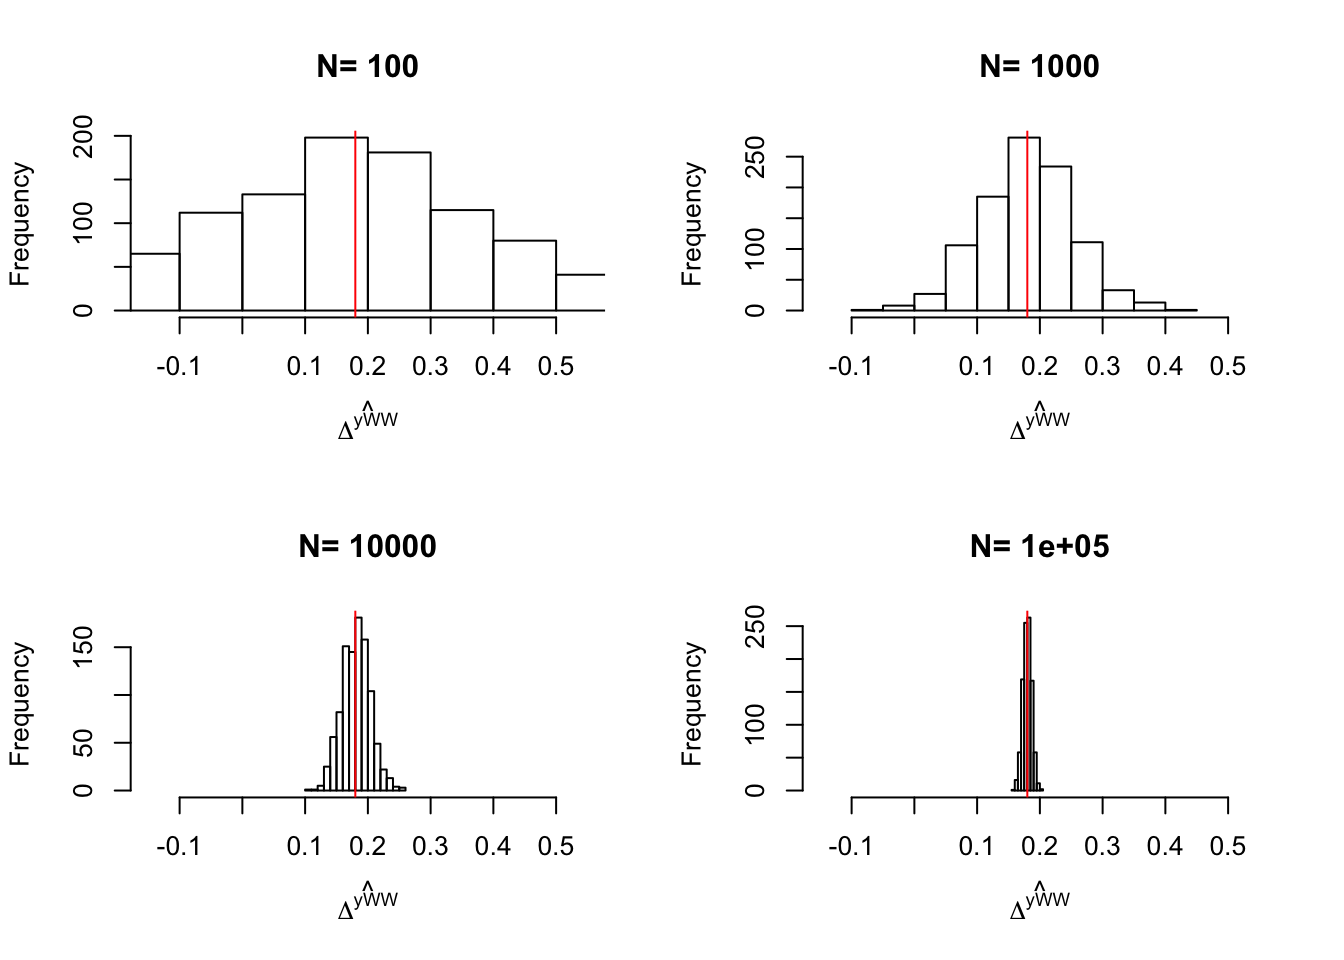
\includegraphics[width=0.6\linewidth]{STCI_files/figure-latex/montecarlo-1} 

}

\caption{Distribution of the $WW$ estimator over replications of samples of different sizes}\label{fig:montecarlo}
\end{figure}

Figure \ref{fig:montecarlo} is essential to understanding statistical inference and the properties of our estimators.
We can see on Figure \ref{fig:montecarlo} that the estimates indeed move around at each sample replication.
We can also see that the estimates seem to be concentrated around the truth.
We also see that the estimates are more and more concentrated around the truth as sample size grows larger and larger.

How big is sampling noise in all of these examples?
We can compute it by using the replications as approximations to the true distribution of the estimator after an infinite number of samples has been drawn.
Let's first choose a confidence level and then compute the empirical equivalent to the formula in Definition \ref{def:sampnoise}.

\begin{Shaded}
\begin{Highlighting}[]
\NormalTok{delta<-}\StringTok{ }\FloatTok{0.99}
\NormalTok{delta}\FloatTok{.2}\NormalTok{ <-}\StringTok{ }\FloatTok{0.95}
\NormalTok{samp.noise <-}\StringTok{ }\ControlFlowTok{function}\NormalTok{(estim,delta)\{}
  \KeywordTok{return}\NormalTok{(}\DecValTok{2}\OperatorTok{*}\KeywordTok{quantile}\NormalTok{(}\KeywordTok{abs}\NormalTok{(}\KeywordTok{delta.y.ate}\NormalTok{(param)}\OperatorTok{-}\NormalTok{estim),}\DataTypeTok{prob=}\NormalTok{delta))}
\NormalTok{\}}
\NormalTok{samp.noise.ww <-}\StringTok{ }\KeywordTok{sapply}\NormalTok{(}\KeywordTok{lapply}\NormalTok{(simuls.ww,}\StringTok{`}\DataTypeTok{[}\StringTok{`}\NormalTok{,,}\DecValTok{1}\NormalTok{),samp.noise,}\DataTypeTok{delta=}\NormalTok{delta)}
\KeywordTok{names}\NormalTok{(samp.noise.ww) <-}\StringTok{ }\NormalTok{N.sample}
\NormalTok{samp.noise.ww}
\end{Highlighting}
\end{Shaded}

\begin{verbatim}
##        100       1000      10000      1e+05 
## 1.09916429 0.39083801 0.11582492 0.03527744
\end{verbatim}

Let's also compute precision and the signal to noise ratio and put all of these results together in a nice table.

\begin{Shaded}
\begin{Highlighting}[]
\NormalTok{precision <-}\StringTok{ }\ControlFlowTok{function}\NormalTok{(estim,delta)\{}
  \KeywordTok{return}\NormalTok{(}\DecValTok{1}\OperatorTok{/}\KeywordTok{samp.noise}\NormalTok{(estim,delta))}
\NormalTok{\}}
\NormalTok{signal.to.noise <-}\StringTok{ }\ControlFlowTok{function}\NormalTok{(estim,delta,param)\{}
  \KeywordTok{return}\NormalTok{(}\KeywordTok{delta.y.ate}\NormalTok{(param)}\OperatorTok{/}\KeywordTok{samp.noise}\NormalTok{(estim,delta))}
\NormalTok{\}}
\NormalTok{precision.ww <-}\StringTok{ }\KeywordTok{sapply}\NormalTok{(}\KeywordTok{lapply}\NormalTok{(simuls.ww,}\StringTok{`}\DataTypeTok{[}\StringTok{`}\NormalTok{,,}\DecValTok{1}\NormalTok{),precision,}\DataTypeTok{delta=}\NormalTok{delta)}
\KeywordTok{names}\NormalTok{(precision.ww) <-}\StringTok{ }\NormalTok{N.sample}
\NormalTok{signal.to.noise.ww <-}\StringTok{ }\KeywordTok{sapply}\NormalTok{(}\KeywordTok{lapply}\NormalTok{(simuls.ww,}\StringTok{`}\DataTypeTok{[}\StringTok{`}\NormalTok{,,}\DecValTok{1}\NormalTok{),signal.to.noise,}\DataTypeTok{delta=}\NormalTok{delta,}\DataTypeTok{param=}\NormalTok{param)}
\KeywordTok{names}\NormalTok{(signal.to.noise.ww) <-}\StringTok{ }\NormalTok{N.sample}
\NormalTok{table.noise <-}\StringTok{ }\KeywordTok{cbind}\NormalTok{(samp.noise.ww,precision.ww,signal.to.noise.ww)}
\KeywordTok{colnames}\NormalTok{(table.noise) <-}\StringTok{ }\KeywordTok{c}\NormalTok{(}\StringTok{'Sampling noise'}\NormalTok{, }\StringTok{'Precision'}\NormalTok{, }\StringTok{'Signal to noise ratio'}\NormalTok{)}
\NormalTok{knitr}\OperatorTok{::}\KeywordTok{kable}\NormalTok{(table.noise,}\DataTypeTok{caption=}\KeywordTok{paste}\NormalTok{(}\StringTok{'Sampling noise of $}\CharTok{\textbackslash{}\textbackslash{}}\StringTok{hat\{WW\}$ for the population treatment effect with $}\CharTok{\textbackslash{}\textbackslash{}}\StringTok{delta=$'}\NormalTok{,delta,}\StringTok{'for various sample sizes'}\NormalTok{,}\DataTypeTok{sep=}\StringTok{' '}\NormalTok{),}\DataTypeTok{booktabs=}\OtherTok{TRUE}\NormalTok{,}\DataTypeTok{digits =} \KeywordTok{c}\NormalTok{(}\DecValTok{2}\NormalTok{,}\DecValTok{2}\NormalTok{,}\DecValTok{2}\NormalTok{),}\DataTypeTok{align=}\KeywordTok{c}\NormalTok{(}\StringTok{'c'}\NormalTok{,}\StringTok{'c'}\NormalTok{,}\StringTok{'c'}\NormalTok{))}
\end{Highlighting}
\end{Shaded}

\begin{table}[t]

\caption{\label{tab:precisionsignal}Sampling noise of $\hat{WW}$ for the population treatment effect with $\delta=$ 0.99 for various sample sizes}
\centering
\begin{tabular}{lccc}
\toprule
  & Sampling noise & Precision & Signal to noise ratio\\
\midrule
100 & 1.10 & 0.91 & 0.16\\
1000 & 0.39 & 2.56 & 0.46\\
10000 & 0.12 & 8.63 & 1.55\\
1e+05 & 0.04 & 28.35 & 5.10\\
\bottomrule
\end{tabular}
\end{table}

Finally, a nice way to summarize the extent of sampling noise is to graph how sampling noise varies around the true treatment effect, as shown on Figure \ref{fig:precision}.

\begin{Shaded}
\begin{Highlighting}[]
\KeywordTok{colnames}\NormalTok{(table.noise) <-}\StringTok{ }\KeywordTok{c}\NormalTok{(}\StringTok{'sampling.noise'}\NormalTok{, }\StringTok{'precision'}\NormalTok{, }\StringTok{'signal.to.noise'}\NormalTok{)}
\NormalTok{table.noise <-}\StringTok{ }\KeywordTok{as.data.frame}\NormalTok{(table.noise)}
\NormalTok{table.noise}\OperatorTok{$}\NormalTok{N <-}\StringTok{ }\KeywordTok{as.numeric}\NormalTok{(}\KeywordTok{rownames}\NormalTok{(table.noise))}
\NormalTok{table.noise}\OperatorTok{$}\NormalTok{TT <-}\StringTok{ }\KeywordTok{rep}\NormalTok{(}\KeywordTok{delta.y.ate}\NormalTok{(param),}\KeywordTok{nrow}\NormalTok{(table.noise))}
\KeywordTok{ggplot}\NormalTok{(table.noise, }\KeywordTok{aes}\NormalTok{(}\DataTypeTok{x=}\KeywordTok{as.factor}\NormalTok{(N), }\DataTypeTok{y=}\NormalTok{TT)) }\OperatorTok{+}
\StringTok{  }\KeywordTok{geom_bar}\NormalTok{(}\DataTypeTok{position=}\KeywordTok{position_dodge}\NormalTok{(), }\DataTypeTok{stat=}\StringTok{"identity"}\NormalTok{, }\DataTypeTok{colour=}\StringTok{'black'}\NormalTok{) }\OperatorTok{+}
\StringTok{  }\KeywordTok{geom_errorbar}\NormalTok{(}\KeywordTok{aes}\NormalTok{(}\DataTypeTok{ymin=}\NormalTok{TT}\OperatorTok{-}\NormalTok{sampling.noise}\OperatorTok{/}\DecValTok{2}\NormalTok{, }\DataTypeTok{ymax=}\NormalTok{TT}\OperatorTok{+}\NormalTok{sampling.noise}\OperatorTok{/}\DecValTok{2}\NormalTok{), }\DataTypeTok{width=}\NormalTok{.}\DecValTok{2}\NormalTok{,}\DataTypeTok{position=}\KeywordTok{position_dodge}\NormalTok{(.}\DecValTok{9}\NormalTok{),}\DataTypeTok{color=}\StringTok{'red'}\NormalTok{) }\OperatorTok{+}
\StringTok{  }\KeywordTok{xlab}\NormalTok{(}\StringTok{"Sample Size"}\NormalTok{)}\OperatorTok{+}
\StringTok{  }\KeywordTok{theme_bw}\NormalTok{()}
\end{Highlighting}
\end{Shaded}

\begin{figure}[htbp]

{\centering 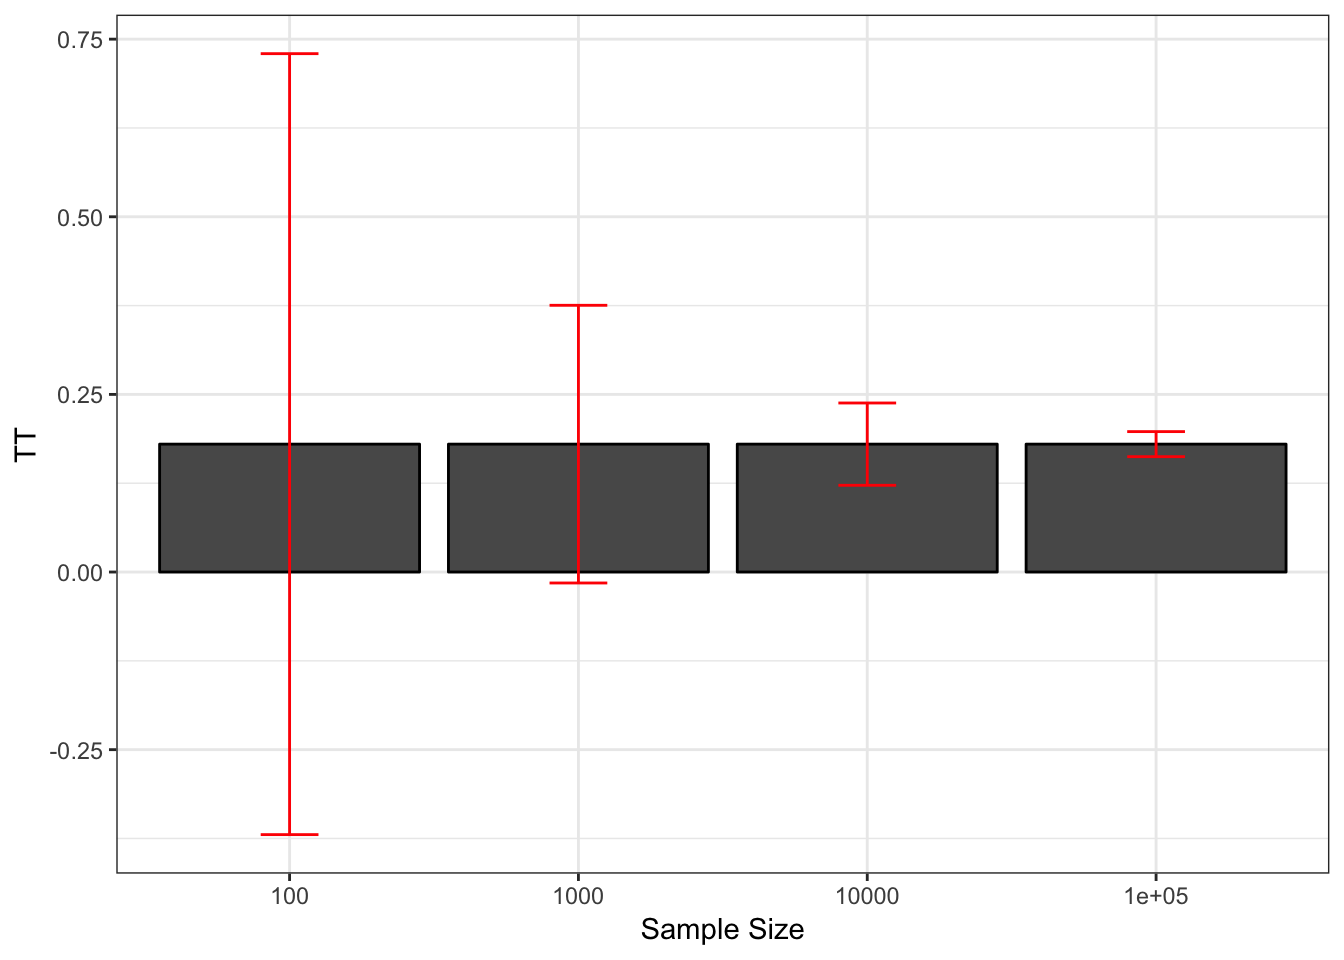
\includegraphics[width=0.6\linewidth]{STCI_files/figure-latex/precision-1} 

}

\caption{Sampling noise of $\hat{WW}$ (99\% confidence) around $TT$ for various sample sizes}\label{fig:precision}
\end{figure}

With \(N=\) 100, we can definitely see on Figure \ref{fig:precision} that sampling noise is ridiculously large, especially compared with the treatment effect that we are trying to estimate.
The signal to noise ratio is 0.16, which means that sampling noise is an order of magnitude bigger than the signal we are trying to extract.
As a consequence, in 22.2\% of our samples, we are going to estimate a negative effect of the treatment.
There is also a 20.4\% chance that we end up estimating an effect that is double the true effect.
So how much can we trust our estimate from one sample to be close to the true effect of the treatment when \(N=\) 100?
Not much.

With \(N=\) 1000, sampling noise is still large: the signal to noise ratio is 0.46, which means that sampling noise is double the signal we are trying to extract.
As a consequence, the chance that we end up with a negative treatment effect has decreased to 0.9\% and that we end up with an effect double the true one is 1\%.
But still, the chances that we end up with an effect that is smaller than three quarters of the true effect is 25.6\% and the chances that we end up with an estimator that is 25\% bigger than the true effect is 26.2\%.
These are nontrivial differences: compare a program that increases earnings by 13.5\% to one that increases them by 18\% and another by 22.5\%.
They would have completely different cost/benefit ratios.
But we at least trust our estimator to give us a correct idea of the sign of the treatment effect and a vague and imprecise idea of its magnitude.

With \(N=\) \ensuremath{10^{4}}, sampling noise is smaller than the signal, which is encouraging.
The signal to noise ratio is 1.55.
In only 1\% of the samples does the estimated effect of the treatment become smaller than 0.125 or bigger than 0.247.
We start gaining a lot of confidence in the relative magnitude of the effect, even if sampling noise is still responsible for economically significant variation.

With \(N=\) \ensuremath{10^{5}}, sampling noise has become trivial.
The signal to noise ratio is 5.1, which means that the signal is now 5 times bigger than the sampling noise.
In only 1\% of the samples does the estimated effect of the treatment become smaller than 0.163 or bigger than 0.198.
Sampling noise is not any more responsible for economically meaningful variation.

\hypertarget{sec:illusnoisesamp}{%
\subsection{Sampling noise for the sample treatment effect}\label{sec:illusnoisesamp}}

Sampling noise for the sample parameter stems from the fact that the treated and control groups are not perfectly identical.
The distribution of observed and unobserved covariates is actually different, because of sampling variation.
This makes the actual comparison of means in the sample a noisy estimate of the true comparison that we would obtain by comparing the potential outcomes of the treated directly.

In order to understand this issue well and to be able to illustrate it correctly, I am going to focus on the average treatment effect in the whole sample, not on the treated: \(\Delta^Y_{ATE_s}=\frac{1}{N}\sum_{i=1}^N(Y_i^1-Y_i^0)\).
This enables me to define a sample parameter that is independent of the allocation of \(D_i\).
This is without important consequences since these two parameters are equal in the population when there is no selection bias, as we are assuming since the beginning of this lecture.
Furthermore, if we view the treatment allocation generating no selection bias as a true random assignment in a Randomized Controlled Trial (RCT), then it is still possible to use this approach to estimate \(TT\) if we view the population over which we randomise as the population selected for receiving the treatment, as we will see in the lecture on RCTs.

\BeginKnitrBlock{example}
\protect\hypertarget{exm:unnamed-chunk-34}{}{\label{exm:unnamed-chunk-34} }In order to assess the scope of sampling noise for our sample treatment effect estimate, we first have to draw a sample:
\EndKnitrBlock{example}

\begin{Shaded}
\begin{Highlighting}[]
\KeywordTok{set.seed}\NormalTok{(}\DecValTok{1234}\NormalTok{)}
\NormalTok{N <-}\DecValTok{1000}
\NormalTok{mu <-}\StringTok{ }\KeywordTok{rnorm}\NormalTok{(N,param[}\StringTok{"barmu"}\NormalTok{],}\KeywordTok{sqrt}\NormalTok{(param[}\StringTok{"sigma2mu"}\NormalTok{]))}
\NormalTok{UB <-}\StringTok{ }\KeywordTok{rnorm}\NormalTok{(N,}\DecValTok{0}\NormalTok{,}\KeywordTok{sqrt}\NormalTok{(param[}\StringTok{"sigma2U"}\NormalTok{]))}
\NormalTok{yB <-}\StringTok{ }\NormalTok{mu }\OperatorTok{+}\StringTok{ }\NormalTok{UB }
\NormalTok{YB <-}\StringTok{ }\KeywordTok{exp}\NormalTok{(yB)}
\NormalTok{Ds <-}\StringTok{ }\KeywordTok{rep}\NormalTok{(}\DecValTok{0}\NormalTok{,N)}
\NormalTok{V <-}\StringTok{ }\KeywordTok{rnorm}\NormalTok{(N,param[}\StringTok{"barmu"}\NormalTok{],}\KeywordTok{sqrt}\NormalTok{(param[}\StringTok{"sigma2mu"}\NormalTok{]}\OperatorTok{+}\NormalTok{param[}\StringTok{"sigma2U"}\NormalTok{]))}
\NormalTok{Ds[V}\OperatorTok{<=}\KeywordTok{log}\NormalTok{(param[}\StringTok{"barY"}\NormalTok{])] <-}\StringTok{ }\DecValTok{1} 
\NormalTok{epsilon <-}\StringTok{ }\KeywordTok{rnorm}\NormalTok{(N,}\DecValTok{0}\NormalTok{,}\KeywordTok{sqrt}\NormalTok{(param[}\StringTok{"sigma2epsilon"}\NormalTok{]))}
\NormalTok{eta<-}\StringTok{ }\KeywordTok{rnorm}\NormalTok{(N,}\DecValTok{0}\NormalTok{,}\KeywordTok{sqrt}\NormalTok{(param[}\StringTok{"sigma2eta"}\NormalTok{]))}
\NormalTok{U0 <-}\StringTok{ }\NormalTok{param[}\StringTok{"rho"}\NormalTok{]}\OperatorTok{*}\NormalTok{UB }\OperatorTok{+}\StringTok{ }\NormalTok{epsilon}
\NormalTok{y0 <-}\StringTok{ }\NormalTok{mu }\OperatorTok{+}\StringTok{  }\NormalTok{U0 }\OperatorTok{+}\StringTok{ }\NormalTok{param[}\StringTok{"delta"}\NormalTok{]}
\NormalTok{alpha <-}\StringTok{ }\NormalTok{param[}\StringTok{"baralpha"}\NormalTok{]}\OperatorTok{+}\StringTok{  }\NormalTok{param[}\StringTok{"theta"}\NormalTok{]}\OperatorTok{*}\NormalTok{mu }\OperatorTok{+}\StringTok{ }\NormalTok{eta}
\NormalTok{y1 <-}\StringTok{ }\NormalTok{y0}\OperatorTok{+}\NormalTok{alpha}
\NormalTok{Y0 <-}\StringTok{ }\KeywordTok{exp}\NormalTok{(y0)}
\NormalTok{Y1 <-}\StringTok{ }\KeywordTok{exp}\NormalTok{(y1)}
\NormalTok{y <-}\StringTok{ }\NormalTok{y1}\OperatorTok{*}\NormalTok{Ds}\OperatorTok{+}\NormalTok{y0}\OperatorTok{*}\NormalTok{(}\DecValTok{1}\OperatorTok{-}\NormalTok{Ds)}
\NormalTok{Y <-}\StringTok{ }\NormalTok{Y1}\OperatorTok{*}\NormalTok{Ds}\OperatorTok{+}\NormalTok{Y0}\OperatorTok{*}\NormalTok{(}\DecValTok{1}\OperatorTok{-}\NormalTok{Ds)}
\end{Highlighting}
\end{Shaded}

In this sample, the treatment effect parameter is \(\Delta^y_{ATE_s}=\) 0.171.
The \(WW\) estimator yields an estimate of \(\hat{\Delta^y_{WW}}=\) 0.133.
Despite random assignment, we have \(\Delta^y_{ATE_s}\neq\hat{\Delta^y_{WW}}\), an instance of the FPSI.

In order to see how sampling noise varies, let's draw a new treatment allocation, while retaining the same sample and the same potential outcomes.

\begin{Shaded}
\begin{Highlighting}[]
\KeywordTok{set.seed}\NormalTok{(}\DecValTok{12345}\NormalTok{)}
\NormalTok{N <-}\DecValTok{1000}
\NormalTok{Ds <-}\StringTok{ }\KeywordTok{rep}\NormalTok{(}\DecValTok{0}\NormalTok{,N)}
\NormalTok{V <-}\StringTok{ }\KeywordTok{rnorm}\NormalTok{(N,param[}\StringTok{"barmu"}\NormalTok{],}\KeywordTok{sqrt}\NormalTok{(param[}\StringTok{"sigma2mu"}\NormalTok{]}\OperatorTok{+}\NormalTok{param[}\StringTok{"sigma2U"}\NormalTok{]))}
\NormalTok{Ds[V}\OperatorTok{<=}\KeywordTok{log}\NormalTok{(param[}\StringTok{"barY"}\NormalTok{])] <-}\StringTok{ }\DecValTok{1} 
\NormalTok{y <-}\StringTok{ }\NormalTok{y1}\OperatorTok{*}\NormalTok{Ds}\OperatorTok{+}\NormalTok{y0}\OperatorTok{*}\NormalTok{(}\DecValTok{1}\OperatorTok{-}\NormalTok{Ds)}
\NormalTok{Y <-}\StringTok{ }\NormalTok{Y1}\OperatorTok{*}\NormalTok{Ds}\OperatorTok{+}\NormalTok{Y0}\OperatorTok{*}\NormalTok{(}\DecValTok{1}\OperatorTok{-}\NormalTok{Ds)}
\end{Highlighting}
\end{Shaded}

In this sample, the treatment effect parameter is still \(\Delta^y_{ATE_s}=\) 0.171.
The \(WW\) estimator yields now an estimate of \(\hat{\Delta^y_{WW}}=\) 0.051.
The \(WW\) estimate is different from our previous estimate because the treatment was allocated to a different random subset of people.

Why is this second estimate so imprecise?
It might because it estimates one of the two components of the average treatment effect badly, or both.
The true average potential outcome with the treatment is, in this sample, \(\frac{1}{N}\sum_{i=1}^Ny_i^1=\) 8.207 while the \(WW\) estimate of this quantity is \(\frac{1}{\sum_{i=1}^ND_i}\sum_{i=1}^ND_iy_i=\) 8.113.
The true average potential outcome without the treatment is, in this sample, \(\frac{1}{N}\sum_{i=1}^Ny_i^0=\) 8.036 while the \(WW\) estimate of this quantity is \(\frac{1}{\sum_{i=1}^N(1-D_i)}\sum_{i=1}^N(1-D_i)y_i=\) 8.062.
It thus seems that most of the bias in the estimated effect stems from the fact that the treatment has been allocated to individuals with lower than expected outcomes with the treatment, be it because they did not react strongly to the treatment, or because they were in worse shape without the treatment.
We can check which one of these two explanations is more important.
The true average effect of the treatment is, in this sample, \(\frac{1}{N}\sum_{i=1}^N(y_i^1-y^0_i)=\) 0.171 while, in the treated group, this quantity is \(\frac{1}{\sum_{i=1}^ND_i}\sum_{i=1}^ND_i(y_i^1-y_i^0)=\) 0.18.
The true average potential outcome without the treatment is, in this sample, \(\frac{1}{N}\sum_{i=1}^Ny^0_i=\) 8.036 while, in the treated group, this quantity is \(\frac{1}{\sum_{i=1}^ND_i}\sum_{i=1}^ND_iy_i^0=\) 7.933.
The reason for the poor performance of the \(WW\) estimator in this sample is that individuals with lower counterfactual outcomes were included in the treated group, not that the treatment had lower effects on them.
The bad counterfactual outcomes of the treated generates a bias of -0.103, while the bias due to heterogeneous reactions to the treatment is of 0.009.
The last part of the bias is the one due to the fact that the individuals in the control group have slightly better counterfactual outcomes than in the sample: -0.026.
The sum of these three terms yields the total bias of our \(WW\) estimator in this second sample: -0.12.

Let's now assess the overall effect of sampling noise on the estimate of the sample treatment effect for various sample sizes.
In order to do this, I am going to use parallelized Monte Carlo simulations again.
For the sake of simplicity, I am going to generate the same potential outcomes in each replication, using the same seed, and only choose a different treatment allocation.

\begin{Shaded}
\begin{Highlighting}[]
\NormalTok{monte.carlo.ww.sample <-}\StringTok{ }\ControlFlowTok{function}\NormalTok{(s,N,param)\{}
  \KeywordTok{set.seed}\NormalTok{(}\DecValTok{1234}\NormalTok{)}
\NormalTok{  mu <-}\StringTok{ }\KeywordTok{rnorm}\NormalTok{(N,param[}\StringTok{"barmu"}\NormalTok{],}\KeywordTok{sqrt}\NormalTok{(param[}\StringTok{"sigma2mu"}\NormalTok{]))}
\NormalTok{  UB <-}\StringTok{ }\KeywordTok{rnorm}\NormalTok{(N,}\DecValTok{0}\NormalTok{,}\KeywordTok{sqrt}\NormalTok{(param[}\StringTok{"sigma2U"}\NormalTok{]))}
\NormalTok{  yB <-}\StringTok{ }\NormalTok{mu }\OperatorTok{+}\StringTok{ }\NormalTok{UB }
\NormalTok{  YB <-}\StringTok{ }\KeywordTok{exp}\NormalTok{(yB)}
\NormalTok{  epsilon <-}\StringTok{ }\KeywordTok{rnorm}\NormalTok{(N,}\DecValTok{0}\NormalTok{,}\KeywordTok{sqrt}\NormalTok{(param[}\StringTok{"sigma2epsilon"}\NormalTok{]))}
\NormalTok{  eta<-}\StringTok{ }\KeywordTok{rnorm}\NormalTok{(N,}\DecValTok{0}\NormalTok{,}\KeywordTok{sqrt}\NormalTok{(param[}\StringTok{"sigma2eta"}\NormalTok{]))}
\NormalTok{  U0 <-}\StringTok{ }\NormalTok{param[}\StringTok{"rho"}\NormalTok{]}\OperatorTok{*}\NormalTok{UB }\OperatorTok{+}\StringTok{ }\NormalTok{epsilon}
\NormalTok{  y0 <-}\StringTok{ }\NormalTok{mu }\OperatorTok{+}\StringTok{  }\NormalTok{U0 }\OperatorTok{+}\StringTok{ }\NormalTok{param[}\StringTok{"delta"}\NormalTok{]}
\NormalTok{  alpha <-}\StringTok{ }\NormalTok{param[}\StringTok{"baralpha"}\NormalTok{]}\OperatorTok{+}\StringTok{  }\NormalTok{param[}\StringTok{"theta"}\NormalTok{]}\OperatorTok{*}\NormalTok{mu }\OperatorTok{+}\StringTok{ }\NormalTok{eta}
\NormalTok{  y1 <-}\StringTok{ }\NormalTok{y0}\OperatorTok{+}\NormalTok{alpha}
\NormalTok{  Y0 <-}\StringTok{ }\KeywordTok{exp}\NormalTok{(y0)}
\NormalTok{  Y1 <-}\StringTok{ }\KeywordTok{exp}\NormalTok{(y1)}
  \KeywordTok{set.seed}\NormalTok{(s)}
\NormalTok{  Ds <-}\StringTok{ }\KeywordTok{rep}\NormalTok{(}\DecValTok{0}\NormalTok{,N)}
\NormalTok{  V <-}\StringTok{ }\KeywordTok{rnorm}\NormalTok{(N,param[}\StringTok{"barmu"}\NormalTok{],}\KeywordTok{sqrt}\NormalTok{(param[}\StringTok{"sigma2mu"}\NormalTok{]}\OperatorTok{+}\NormalTok{param[}\StringTok{"sigma2U"}\NormalTok{]))}
\NormalTok{  Ds[V}\OperatorTok{<=}\KeywordTok{log}\NormalTok{(param[}\StringTok{"barY"}\NormalTok{])] <-}\StringTok{ }\DecValTok{1} 
\NormalTok{  y <-}\StringTok{ }\NormalTok{y1}\OperatorTok{*}\NormalTok{Ds}\OperatorTok{+}\NormalTok{y0}\OperatorTok{*}\NormalTok{(}\DecValTok{1}\OperatorTok{-}\NormalTok{Ds)}
\NormalTok{  Y <-}\StringTok{ }\NormalTok{Y1}\OperatorTok{*}\NormalTok{Ds}\OperatorTok{+}\NormalTok{Y0}\OperatorTok{*}\NormalTok{(}\DecValTok{1}\OperatorTok{-}\NormalTok{Ds)}
  \KeywordTok{return}\NormalTok{((}\DecValTok{1}\OperatorTok{/}\KeywordTok{sum}\NormalTok{(Ds))}\OperatorTok{*}\KeywordTok{sum}\NormalTok{(y}\OperatorTok{*}\NormalTok{Ds)}\OperatorTok{-}\NormalTok{(}\DecValTok{1}\OperatorTok{/}\KeywordTok{sum}\NormalTok{(}\DecValTok{1}\OperatorTok{-}\NormalTok{Ds))}\OperatorTok{*}\KeywordTok{sum}\NormalTok{(y}\OperatorTok{*}\NormalTok{(}\DecValTok{1}\OperatorTok{-}\NormalTok{Ds)))}
\NormalTok{\}}

\NormalTok{simuls.ww.N.sample <-}\StringTok{ }\ControlFlowTok{function}\NormalTok{(N,Nsim,param)\{}
  \KeywordTok{return}\NormalTok{(}\KeywordTok{unlist}\NormalTok{(}\KeywordTok{lapply}\NormalTok{(}\DecValTok{1}\OperatorTok{:}\NormalTok{Nsim,monte.carlo.ww.sample,}\DataTypeTok{N=}\NormalTok{N,}\DataTypeTok{param=}\NormalTok{param)))}
\NormalTok{\}}

\NormalTok{sf.simuls.ww.N.sample <-}\StringTok{ }\ControlFlowTok{function}\NormalTok{(N,Nsim,param)\{}
  \KeywordTok{sfInit}\NormalTok{(}\DataTypeTok{parallel=}\OtherTok{TRUE}\NormalTok{,}\DataTypeTok{cpus=}\NormalTok{ncpus)}
\NormalTok{  sim <-}\StringTok{ }\KeywordTok{sfLapply}\NormalTok{(}\DecValTok{1}\OperatorTok{:}\NormalTok{Nsim,monte.carlo.ww.sample,}\DataTypeTok{N=}\NormalTok{N,}\DataTypeTok{param=}\NormalTok{param)}
  \KeywordTok{sfStop}\NormalTok{()}
  \KeywordTok{return}\NormalTok{(}\KeywordTok{unlist}\NormalTok{(sim))}
\NormalTok{\}}

\NormalTok{simuls.ww.sample <-}\StringTok{ }\KeywordTok{lapply}\NormalTok{(N.sample,sf.simuls.ww.N.sample,}\DataTypeTok{Nsim=}\NormalTok{Nsim,}\DataTypeTok{param=}\NormalTok{param)}

\NormalTok{monte.carlo.ate.sample <-}\StringTok{ }\ControlFlowTok{function}\NormalTok{(N,s,param)\{}
  \KeywordTok{set.seed}\NormalTok{(s)}
\NormalTok{  mu <-}\StringTok{ }\KeywordTok{rnorm}\NormalTok{(N,param[}\StringTok{"barmu"}\NormalTok{],}\KeywordTok{sqrt}\NormalTok{(param[}\StringTok{"sigma2mu"}\NormalTok{]))}
\NormalTok{  UB <-}\StringTok{ }\KeywordTok{rnorm}\NormalTok{(N,}\DecValTok{0}\NormalTok{,}\KeywordTok{sqrt}\NormalTok{(param[}\StringTok{"sigma2U"}\NormalTok{]))}
\NormalTok{  yB <-}\StringTok{ }\NormalTok{mu }\OperatorTok{+}\StringTok{ }\NormalTok{UB }
\NormalTok{  YB <-}\StringTok{ }\KeywordTok{exp}\NormalTok{(yB)}
\NormalTok{  epsilon <-}\StringTok{ }\KeywordTok{rnorm}\NormalTok{(N,}\DecValTok{0}\NormalTok{,}\KeywordTok{sqrt}\NormalTok{(param[}\StringTok{"sigma2epsilon"}\NormalTok{]))}
\NormalTok{  eta<-}\StringTok{ }\KeywordTok{rnorm}\NormalTok{(N,}\DecValTok{0}\NormalTok{,}\KeywordTok{sqrt}\NormalTok{(param[}\StringTok{"sigma2eta"}\NormalTok{]))}
\NormalTok{  U0 <-}\StringTok{ }\NormalTok{param[}\StringTok{"rho"}\NormalTok{]}\OperatorTok{*}\NormalTok{UB }\OperatorTok{+}\StringTok{ }\NormalTok{epsilon}
\NormalTok{  y0 <-}\StringTok{ }\NormalTok{mu }\OperatorTok{+}\StringTok{  }\NormalTok{U0 }\OperatorTok{+}\StringTok{ }\NormalTok{param[}\StringTok{"delta"}\NormalTok{]}
\NormalTok{  alpha <-}\StringTok{ }\NormalTok{param[}\StringTok{"baralpha"}\NormalTok{]}\OperatorTok{+}\StringTok{  }\NormalTok{param[}\StringTok{"theta"}\NormalTok{]}\OperatorTok{*}\NormalTok{mu }\OperatorTok{+}\StringTok{ }\NormalTok{eta}
\NormalTok{  y1 <-}\StringTok{ }\NormalTok{y0}\OperatorTok{+}\NormalTok{alpha}
\NormalTok{  Y0 <-}\StringTok{ }\KeywordTok{exp}\NormalTok{(y0)}
\NormalTok{  Y1 <-}\StringTok{ }\KeywordTok{exp}\NormalTok{(y1)}
\NormalTok{  Ds <-}\StringTok{ }\KeywordTok{rep}\NormalTok{(}\DecValTok{0}\NormalTok{,N)}
\NormalTok{  V <-}\StringTok{ }\KeywordTok{rnorm}\NormalTok{(N,param[}\StringTok{"barmu"}\NormalTok{],}\KeywordTok{sqrt}\NormalTok{(param[}\StringTok{"sigma2mu"}\NormalTok{]}\OperatorTok{+}\NormalTok{param[}\StringTok{"sigma2U"}\NormalTok{]))}
\NormalTok{  Ds[V}\OperatorTok{<=}\KeywordTok{log}\NormalTok{(param[}\StringTok{"barY"}\NormalTok{])] <-}\StringTok{ }\DecValTok{1} 
\NormalTok{  y <-}\StringTok{ }\NormalTok{y1}\OperatorTok{*}\NormalTok{Ds}\OperatorTok{+}\NormalTok{y0}\OperatorTok{*}\NormalTok{(}\DecValTok{1}\OperatorTok{-}\NormalTok{Ds)}
\NormalTok{  Y <-}\StringTok{ }\NormalTok{Y1}\OperatorTok{*}\NormalTok{Ds}\OperatorTok{+}\NormalTok{Y0}\OperatorTok{*}\NormalTok{(}\DecValTok{1}\OperatorTok{-}\NormalTok{Ds)}
  \KeywordTok{return}\NormalTok{(}\KeywordTok{mean}\NormalTok{(alpha))}
\NormalTok{\}}

\KeywordTok{par}\NormalTok{(}\DataTypeTok{mfrow=}\KeywordTok{c}\NormalTok{(}\DecValTok{2}\NormalTok{,}\DecValTok{2}\NormalTok{))}
\ControlFlowTok{for}\NormalTok{ (i }\ControlFlowTok{in} \DecValTok{1}\OperatorTok{:}\DecValTok{4}\NormalTok{)\{}
  \KeywordTok{hist}\NormalTok{(simuls.ww.sample[[i]],}\DataTypeTok{main=}\KeywordTok{paste}\NormalTok{(}\StringTok{'N='}\NormalTok{,}\KeywordTok{as.character}\NormalTok{(N.sample[i])),}\DataTypeTok{xlab=}\KeywordTok{expression}\NormalTok{(}\KeywordTok{hat}\NormalTok{(Delta}\OperatorTok{^}\NormalTok{yWW)),}\DataTypeTok{xlim=}\KeywordTok{c}\NormalTok{(}\OperatorTok{-}\FloatTok{0.15}\NormalTok{,}\FloatTok{0.55}\NormalTok{))}
  \KeywordTok{abline}\NormalTok{(}\DataTypeTok{v=}\KeywordTok{monte.carlo.ate.sample}\NormalTok{(N.sample[[i]],}\DecValTok{1234}\NormalTok{,param),}\DataTypeTok{col=}\StringTok{"red"}\NormalTok{)}
\NormalTok{\}}
\end{Highlighting}
\end{Shaded}

\begin{figure}[htbp]

{\centering 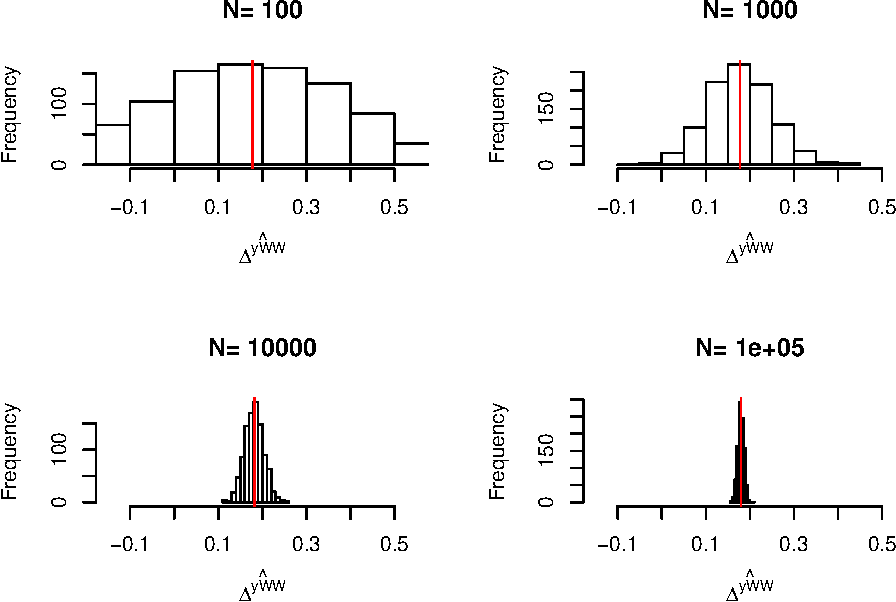
\includegraphics[width=0.6\linewidth]{STCI_files/figure-latex/montecarlosample-1} 

}

\caption{Distribution of the $WW$ estimator over replications of treatment allocation for samples of different sizes}\label{fig:montecarlosample}
\end{figure}

Let's also compute sampling noise, precision and the signal to noise ratio in these examples.

\begin{Shaded}
\begin{Highlighting}[]
\NormalTok{samp.noise.sample <-}\StringTok{ }\ControlFlowTok{function}\NormalTok{(i,delta,param)\{}
  \KeywordTok{return}\NormalTok{(}\DecValTok{2}\OperatorTok{*}\KeywordTok{quantile}\NormalTok{(}\KeywordTok{abs}\NormalTok{(}\KeywordTok{monte.carlo.ate.sample}\NormalTok{(}\DecValTok{1234}\NormalTok{,N.sample[[i]],param)}\OperatorTok{-}\NormalTok{simuls.ww.sample[[i]]),}\DataTypeTok{prob=}\NormalTok{delta))}
\NormalTok{\}}
\NormalTok{samp.noise.ww.sample <-}\StringTok{ }\KeywordTok{sapply}\NormalTok{(}\DecValTok{1}\OperatorTok{:}\DecValTok{4}\NormalTok{,samp.noise.sample,}\DataTypeTok{delta=}\NormalTok{delta,}\DataTypeTok{param=}\NormalTok{param)}
\KeywordTok{names}\NormalTok{(samp.noise.ww.sample) <-}\StringTok{ }\NormalTok{N.sample}

\NormalTok{precision.sample <-}\StringTok{ }\ControlFlowTok{function}\NormalTok{(i,delta,param)\{}
  \KeywordTok{return}\NormalTok{(}\DecValTok{1}\OperatorTok{/}\KeywordTok{samp.noise.sample}\NormalTok{(i,delta,}\DataTypeTok{param=}\NormalTok{param))}
\NormalTok{\}}
\NormalTok{signal.to.noise.sample <-}\StringTok{ }\ControlFlowTok{function}\NormalTok{(i,delta,param)\{}
  \KeywordTok{return}\NormalTok{(}\KeywordTok{monte.carlo.ate.sample}\NormalTok{(}\DecValTok{1234}\NormalTok{,N.sample[[i]],param)}\OperatorTok{/}\KeywordTok{samp.noise.sample}\NormalTok{(i,delta,}\DataTypeTok{param=}\NormalTok{param))}
\NormalTok{\}}
\NormalTok{precision.ww.sample <-}\StringTok{ }\KeywordTok{sapply}\NormalTok{(}\DecValTok{1}\OperatorTok{:}\DecValTok{4}\NormalTok{,precision.sample,}\DataTypeTok{delta=}\NormalTok{delta,}\DataTypeTok{param=}\NormalTok{param)}
\KeywordTok{names}\NormalTok{(precision.ww.sample) <-}\StringTok{ }\NormalTok{N.sample}
\NormalTok{signal.to.noise.ww.sample <-}\StringTok{ }\KeywordTok{sapply}\NormalTok{(}\DecValTok{1}\OperatorTok{:}\DecValTok{4}\NormalTok{,signal.to.noise.sample,}\DataTypeTok{delta=}\NormalTok{delta,}\DataTypeTok{param=}\NormalTok{param)}
\KeywordTok{names}\NormalTok{(signal.to.noise.ww.sample) <-}\StringTok{ }\NormalTok{N.sample}
\NormalTok{table.noise.sample <-}\StringTok{ }\KeywordTok{cbind}\NormalTok{(samp.noise.ww.sample,precision.ww.sample,signal.to.noise.ww.sample)}
\KeywordTok{colnames}\NormalTok{(table.noise.sample) <-}\StringTok{ }\KeywordTok{c}\NormalTok{(}\StringTok{'Sampling noise'}\NormalTok{, }\StringTok{'Precision'}\NormalTok{, }\StringTok{'Signal to noise ratio'}\NormalTok{)}
\NormalTok{knitr}\OperatorTok{::}\KeywordTok{kable}\NormalTok{(table.noise.sample,}\DataTypeTok{caption=}\KeywordTok{paste}\NormalTok{(}\StringTok{'Sampling noise of $}\CharTok{\textbackslash{}\textbackslash{}}\StringTok{hat\{WW\}$ for the sample treatment effect with $}\CharTok{\textbackslash{}\textbackslash{}}\StringTok{delta=$'}\NormalTok{,delta,}\StringTok{'and for various sample sizes'}\NormalTok{,}\DataTypeTok{sep=}\StringTok{' '}\NormalTok{),}\DataTypeTok{booktabs=}\OtherTok{TRUE}\NormalTok{,}\DataTypeTok{align=}\KeywordTok{c}\NormalTok{(}\StringTok{'c'}\NormalTok{,}\StringTok{'c'}\NormalTok{,}\StringTok{'c'}\NormalTok{),}\DataTypeTok{digits=}\KeywordTok{c}\NormalTok{(}\DecValTok{3}\NormalTok{,}\DecValTok{3}\NormalTok{,}\DecValTok{3}\NormalTok{))}
\end{Highlighting}
\end{Shaded}

\begin{table}[t]

\caption{\label{tab:sampnoisesample}Sampling noise of $\hat{WW}$ for the sample treatment effect with $\delta=$ 0.99 and for various sample sizes}
\centering
\begin{tabular}{lccc}
\toprule
  & Sampling noise & Precision & Signal to noise ratio\\
\midrule
100 & 1.208 & 0.828 & 0.149\\
1000 & 0.366 & 2.729 & 0.482\\
10000 & 0.122 & 8.218 & 1.585\\
1e+05 & 0.033 & 30.283 & 5.453\\
\bottomrule
\end{tabular}
\end{table}

Finally, let's compare the extent of sampling noise for the population and the sample treatment effect parameters.

\begin{Shaded}
\begin{Highlighting}[]
\KeywordTok{colnames}\NormalTok{(table.noise.sample) <-}\StringTok{ }\KeywordTok{c}\NormalTok{(}\StringTok{'sampling.noise'}\NormalTok{, }\StringTok{'precision'}\NormalTok{, }\StringTok{'signal.to.noise'}\NormalTok{)}
\NormalTok{table.noise.sample <-}\StringTok{ }\KeywordTok{as.data.frame}\NormalTok{(table.noise.sample)}
\NormalTok{table.noise.sample}\OperatorTok{$}\NormalTok{N <-}\StringTok{ }\KeywordTok{as.numeric}\NormalTok{(}\KeywordTok{rownames}\NormalTok{(table.noise.sample))}
\NormalTok{table.noise.sample}\OperatorTok{$}\NormalTok{TT <-}\StringTok{ }\KeywordTok{sapply}\NormalTok{(N.sample,monte.carlo.ate.sample,}\DataTypeTok{s=}\DecValTok{1234}\NormalTok{,}\DataTypeTok{param=}\NormalTok{param)}
\NormalTok{table.noise.sample}\OperatorTok{$}\NormalTok{Type <-}\StringTok{ 'TTs'}
\NormalTok{table.noise}\OperatorTok{$}\NormalTok{Type <-}\StringTok{ 'TT'}
\NormalTok{table.noise.tot <-}\StringTok{ }\KeywordTok{rbind}\NormalTok{(table.noise,table.noise.sample)}
\NormalTok{table.noise.tot}\OperatorTok{$}\NormalTok{Type <-}\StringTok{ }\KeywordTok{factor}\NormalTok{(table.noise.tot}\OperatorTok{$}\NormalTok{Type)}

\KeywordTok{ggplot}\NormalTok{(table.noise.tot, }\KeywordTok{aes}\NormalTok{(}\DataTypeTok{x=}\KeywordTok{as.factor}\NormalTok{(N), }\DataTypeTok{y=}\NormalTok{TT,}\DataTypeTok{fill=}\NormalTok{Type)) }\OperatorTok{+}
\StringTok{  }\KeywordTok{geom_bar}\NormalTok{(}\DataTypeTok{position=}\KeywordTok{position_dodge}\NormalTok{(), }\DataTypeTok{stat=}\StringTok{"identity"}\NormalTok{, }\DataTypeTok{colour=}\StringTok{'black'}\NormalTok{) }\OperatorTok{+}
\StringTok{  }\KeywordTok{geom_errorbar}\NormalTok{(}\KeywordTok{aes}\NormalTok{(}\DataTypeTok{ymin=}\NormalTok{TT}\OperatorTok{-}\NormalTok{sampling.noise}\OperatorTok{/}\DecValTok{2}\NormalTok{, }\DataTypeTok{ymax=}\NormalTok{TT}\OperatorTok{+}\NormalTok{sampling.noise}\OperatorTok{/}\DecValTok{2}\NormalTok{), }\DataTypeTok{width=}\NormalTok{.}\DecValTok{2}\NormalTok{,}\DataTypeTok{position=}\KeywordTok{position_dodge}\NormalTok{(.}\DecValTok{9}\NormalTok{),}\DataTypeTok{color=}\StringTok{'red'}\NormalTok{) }\OperatorTok{+}
\StringTok{  }\KeywordTok{xlab}\NormalTok{(}\StringTok{"Sample Size"}\NormalTok{)}\OperatorTok{+}
\StringTok{  }\KeywordTok{theme_bw}\NormalTok{()}\OperatorTok{+}
\StringTok{  }\KeywordTok{theme}\NormalTok{(}\DataTypeTok{legend.position=}\KeywordTok{c}\NormalTok{(}\FloatTok{0.85}\NormalTok{,}\FloatTok{0.88}\NormalTok{))}
\end{Highlighting}
\end{Shaded}

\begin{figure}[htbp]

{\centering 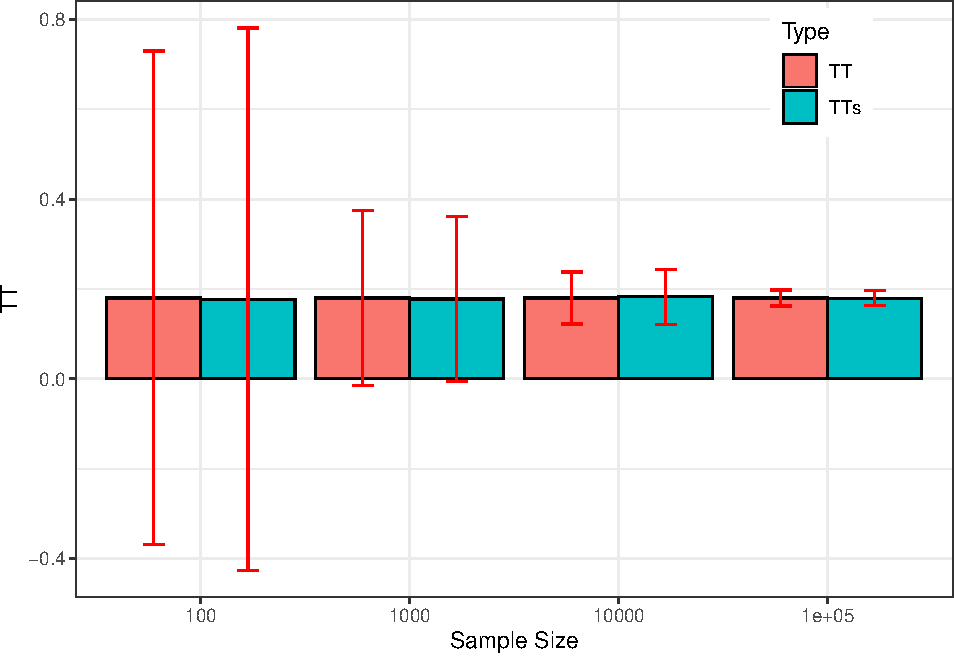
\includegraphics[width=0.6\linewidth]{STCI_files/figure-latex/precisionpopsample-1} 

}

\caption{Sampling noise of $\hat{WW}$ (99\% confidence) around $TT$ and $TT_s$ for various sample sizes}\label{fig:precisionpopsample}
\end{figure}

Figure \ref{fig:montecarlosample} and Table \ref{tab:sampnoisesample} present the results of the simulations of sampling noise for the sample treatment effect parameter.
Figure \ref{fig:precisionpopsample} compares sampling noise for the population and sample treatment effects.\\
For all practical purposes, the estimates of sampling noise for the sample treatment effect are extremely close to the ones we have estimated for the population treatment effect.
I am actually surprised by this result, since I expected that keeping the potential outcomes constant over replications would decrease sampling noise.
It seems that the variability in potential outcomes over replications of random allocations of the treatment in a given sample mimicks very well the sampling process from a population.
I do not know if this result of similarity of sampling noise for the population and sample treatment effect is a general one, but considering them as similar or close seems innocuous in our example.

\hypertarget{sec:confinterv}{%
\subsection{Building confidence intervals from estimates of sampling noise}\label{sec:confinterv}}

In real life, we do not observe \(TT\).
We only have access to \(\hat{E}\).
Let's also assume for now that we have access to an estimate of sampling noise, \(2\epsilon\).
How can we use these two quantities to assess the set of values that \(TT\) might take?
One very useful device that we can use is the confidence interval.
Confidence intervals are very useful because they quantify the zone within which we have a chance to find the true effect \(TT\):

\BeginKnitrBlock{theorem}[Confidence interval]
\protect\hypertarget{thm:confinter}{}{\label{thm:confinter} \iffalse (Confidence interval) \fi{} }For a given level of confidence \(\delta\) and corresponding level of sampling noise \(2\epsilon\) of the estimator \(\hat{E}\) of \(TT\), the confidence interval \(\left\{\hat{E}-\epsilon,\hat{E}+\epsilon\right\}\) is such that the probability that it contains \(TT\) is equal to \(\delta\) over sample replications:
\begin{align*}
  \Pr(\hat{E}-\epsilon\leq TT\leq\hat{E}+\epsilon) & = \delta.
\end{align*}
\EndKnitrBlock{theorem}

\BeginKnitrBlock{proof}
\iffalse{} {Proof. } \fi{}From the definition of sampling noise, we know that:
\begin{align*}
  \Pr(|\hat{E}-TT|\leq\epsilon) & = \delta.
\end{align*}
Now:
\begin{align*}
  \Pr(|\hat{E}-TT|\leq\epsilon) & = \Pr(TT-\epsilon\leq\hat{E}\leq TT+\epsilon)\\
                                & = \Pr(-\hat{E}-\epsilon\leq-TT\leq -\hat{E}+\epsilon)\\
                                & = \Pr(\hat{E}-\epsilon\leq TT\leq\hat{E}+\epsilon),
\end{align*}
which proves the result.
\EndKnitrBlock{proof}

It is very important to note that confidence intervals are centered around \(\hat{E}\) and not around \(TT\).
When estimating sampling noise and building Figure \ref{fig:precision}, we have centered our intervals around \(TT\).
The interval was fixed and \(\hat{E}\) was moving across replications and \(2\epsilon\) was defined as the length of the interval around \(TT\) containing a proportion \(\delta\) of the estimates \(\hat{E}\).
A confidence interval cannot be centered around \(TT\), which is unknown, but is centered around \(\hat{E}\), that we can observe.
As a consequence, it is the interval that moves around across replications, and \(\delta\) is the proportion of samples in which the interval contains \(TT\).

\BeginKnitrBlock{example}
\protect\hypertarget{exm:unnamed-chunk-36}{}{\label{exm:unnamed-chunk-36} }Let's see how confidence intervals behave in our numerical example.
\EndKnitrBlock{example}

\begin{Shaded}
\begin{Highlighting}[]
\NormalTok{N.plot <-}\StringTok{ }\DecValTok{40}
\NormalTok{plot.list <-}\StringTok{ }\KeywordTok{list}\NormalTok{()}

\ControlFlowTok{for}\NormalTok{ (k }\ControlFlowTok{in} \DecValTok{1}\OperatorTok{:}\KeywordTok{length}\NormalTok{(N.sample))\{}
  \KeywordTok{set.seed}\NormalTok{(}\DecValTok{1234}\NormalTok{)}
\NormalTok{  test <-}\StringTok{ }\KeywordTok{sample}\NormalTok{(simuls.ww[[k]][,}\StringTok{'WW'}\NormalTok{],N.plot)}
\NormalTok{  test <-}\StringTok{ }\KeywordTok{as.data.frame}\NormalTok{(}\KeywordTok{cbind}\NormalTok{(test,}\KeywordTok{rep}\NormalTok{(}\KeywordTok{samp.noise}\NormalTok{(simuls.ww[[k]][,}\StringTok{'WW'}\NormalTok{],}\DataTypeTok{delta=}\NormalTok{delta)),}\KeywordTok{rep}\NormalTok{(}\KeywordTok{samp.noise}\NormalTok{(simuls.ww[[k]][,}\StringTok{'WW'}\NormalTok{],}\DataTypeTok{delta=}\NormalTok{delta}\FloatTok{.2}\NormalTok{))))}
  \KeywordTok{colnames}\NormalTok{(test) <-}\StringTok{ }\KeywordTok{c}\NormalTok{(}\StringTok{'WW'}\NormalTok{,}\StringTok{'sampling.noise.1'}\NormalTok{,}\StringTok{'sampling.noise.2'}\NormalTok{)}
\NormalTok{  test}\OperatorTok{$}\NormalTok{id <-}\StringTok{ }\DecValTok{1}\OperatorTok{:}\NormalTok{N.plot}
\NormalTok{  plot.test <-}\StringTok{ }\KeywordTok{ggplot}\NormalTok{(test, }\KeywordTok{aes}\NormalTok{(}\DataTypeTok{x=}\KeywordTok{as.factor}\NormalTok{(id), }\DataTypeTok{y=}\NormalTok{WW)) }\OperatorTok{+}
\StringTok{      }\KeywordTok{geom_bar}\NormalTok{(}\DataTypeTok{position=}\KeywordTok{position_dodge}\NormalTok{(), }\DataTypeTok{stat=}\StringTok{"identity"}\NormalTok{, }\DataTypeTok{colour=}\StringTok{'black'}\NormalTok{) }\OperatorTok{+}
\StringTok{      }\KeywordTok{geom_errorbar}\NormalTok{(}\KeywordTok{aes}\NormalTok{(}\DataTypeTok{ymin=}\NormalTok{WW}\OperatorTok{-}\NormalTok{sampling.noise}\FloatTok{.1}\OperatorTok{/}\DecValTok{2}\NormalTok{, }\DataTypeTok{ymax=}\NormalTok{WW}\OperatorTok{+}\NormalTok{sampling.noise}\FloatTok{.1}\OperatorTok{/}\DecValTok{2}\NormalTok{), }\DataTypeTok{width=}\NormalTok{.}\DecValTok{2}\NormalTok{,}\DataTypeTok{position=}\KeywordTok{position_dodge}\NormalTok{(.}\DecValTok{9}\NormalTok{),}\DataTypeTok{color=}\StringTok{'red'}\NormalTok{) }\OperatorTok{+}
\StringTok{      }\KeywordTok{geom_errorbar}\NormalTok{(}\KeywordTok{aes}\NormalTok{(}\DataTypeTok{ymin=}\NormalTok{WW}\OperatorTok{-}\NormalTok{sampling.noise}\FloatTok{.2}\OperatorTok{/}\DecValTok{2}\NormalTok{, }\DataTypeTok{ymax=}\NormalTok{WW}\OperatorTok{+}\NormalTok{sampling.noise}\FloatTok{.2}\OperatorTok{/}\DecValTok{2}\NormalTok{), }\DataTypeTok{width=}\NormalTok{.}\DecValTok{2}\NormalTok{,}\DataTypeTok{position=}\KeywordTok{position_dodge}\NormalTok{(.}\DecValTok{9}\NormalTok{),}\DataTypeTok{color=}\StringTok{'blue'}\NormalTok{) }\OperatorTok{+}
\StringTok{      }\KeywordTok{geom_hline}\NormalTok{(}\KeywordTok{aes}\NormalTok{(}\DataTypeTok{yintercept=}\KeywordTok{delta.y.ate}\NormalTok{(param)), }\DataTypeTok{colour=}\StringTok{"#990000"}\NormalTok{, }\DataTypeTok{linetype=}\StringTok{"dashed"}\NormalTok{)}\OperatorTok{+}
\StringTok{      }\CommentTok{#ylim(-0.5,1.2)+}
\StringTok{      }\KeywordTok{xlab}\NormalTok{(}\StringTok{"Sample id"}\NormalTok{)}\OperatorTok{+}
\StringTok{      }\KeywordTok{theme_bw}\NormalTok{()}\OperatorTok{+}
\StringTok{      }\KeywordTok{ggtitle}\NormalTok{(}\KeywordTok{paste}\NormalTok{(}\StringTok{"N="}\NormalTok{,N.sample[k]))}
\NormalTok{  plot.list[[k]] <-}\StringTok{ }\NormalTok{plot.test }
\NormalTok{\}}
\NormalTok{plot.CI <-}\StringTok{ }\KeywordTok{plot_grid}\NormalTok{(plot.list[[}\DecValTok{1}\NormalTok{]],plot.list[[}\DecValTok{2}\NormalTok{]],plot.list[[}\DecValTok{3}\NormalTok{]],plot.list[[}\DecValTok{4}\NormalTok{]],}\DataTypeTok{ncol=}\DecValTok{1}\NormalTok{,}\DataTypeTok{nrow=}\KeywordTok{length}\NormalTok{(N.sample))}
\KeywordTok{print}\NormalTok{(plot.CI)}
\end{Highlighting}
\end{Shaded}

\begin{figure}[htbp]

{\centering 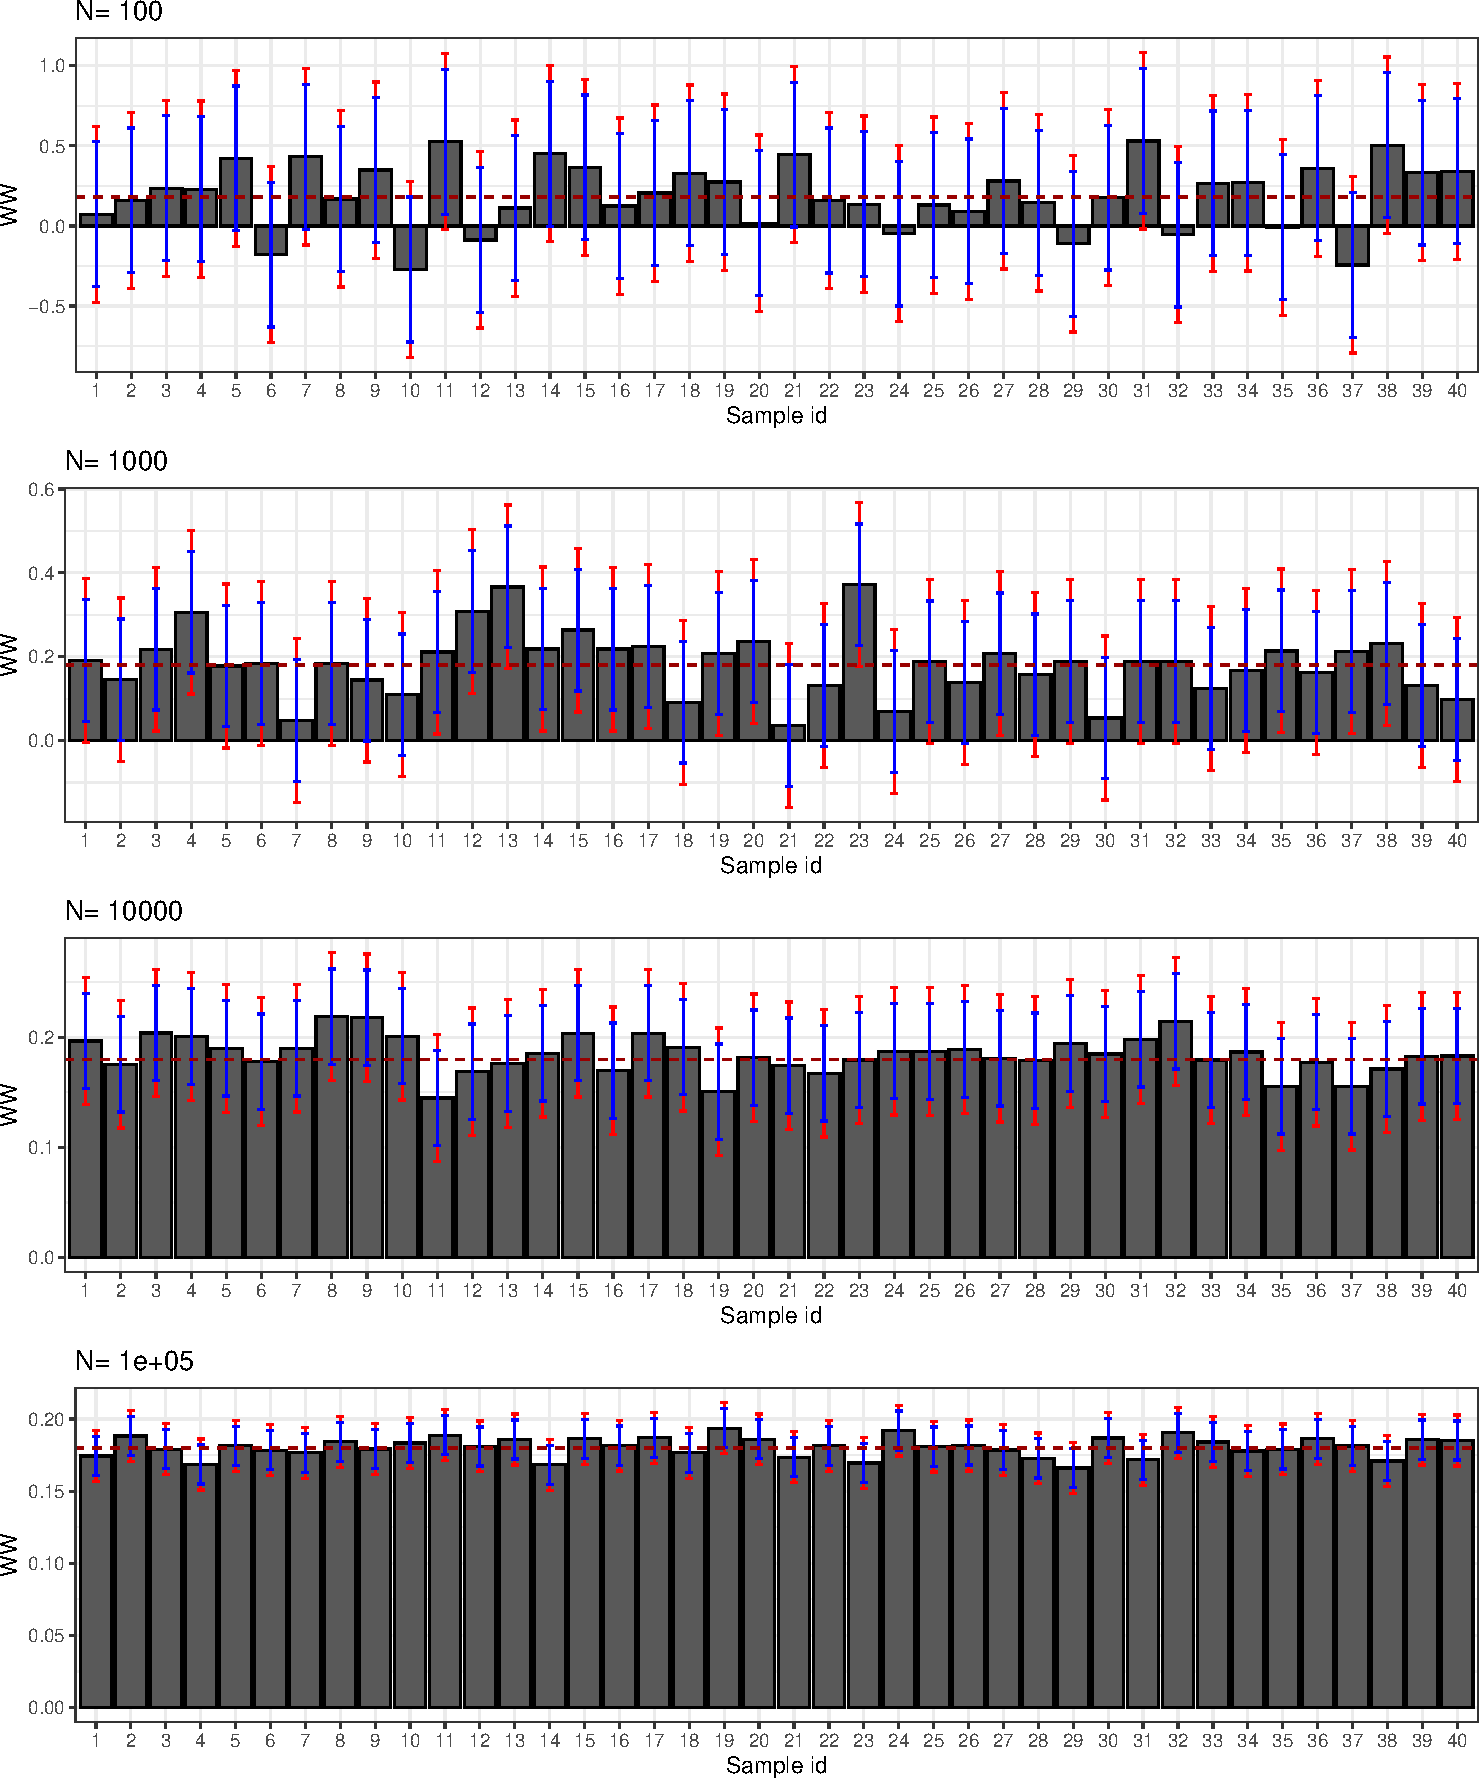
\includegraphics[width=0.6\linewidth]{STCI_files/figure-latex/confinterval-1} 

}

\caption{Confidence intervals of $\hat{WW}$ for $\delta=$ 0.99 (red) and 0.95 (blue) over sample replications for various sample sizes}\label{fig:confinterval}
\end{figure}

Figure \ref{fig:confinterval} presents the 99\% and 95\% confidence intervals for 40 samples selected from our simulations.
First, confidence intervals do their job: they contain the true effect most of the time.
Second, the 95\% confidence interval misses the true effect more often, as expected.
For example, with \(N=\) 1000, the confidence intervals in samples 13 and 23 do not contain the true effect, but it is not far from their lower bound.
Third, confidence intervals faithfully reflect what we can learn from our estimates at each sample size.
With \(N=\) 100, the confidence intervals make it clear that the effect might be very large or very small, even strongly negative.
With \(N=\) 1000, the confidence intervals suggest that the effect is either positive or null, but unlikely to be strongly negative.
Most of the time, we get the sign right.
With \(N=\) \ensuremath{10^{4}}, we know that the true effect is bigger than 0.1 and smaller than 0.3 and most intervals place the true effect somewhere between 0.11 and 0.25.
With \(N=\) \ensuremath{10^{5}}, we know that the true effect is bigger than 0.15 and smaller than 0.21 and most intervals place the true effect somewhere between 0.16 and 0.20.

\hypertarget{reporting-sampling-noise-a-proposal}{%
\subsection{Reporting sampling noise: a proposal}\label{reporting-sampling-noise-a-proposal}}

Once sampling noise is measured (and we'll see how to get an estimate in the next section), one still has to communicate it to others.
There are many ways to report sampling noise:

\begin{itemize}
\tightlist
\item
  Sampling noise as defined in this book (\(2*\epsilon\))
\item
  The corresponding confidence interval
\item
  The signal to noise ratio
\item
  A standard error
\item
  A significance level
\item
  A p-value
\item
  A t-statistic
\end{itemize}

The main problem with all of these approaches is that they do not express sampling noise in a way that is directly comparable to the magnitude of the \(TT\) estimate.
Other ways of reporting sampling noise such as p-values and t-stats are nonlinear transforms of sampling noise, making it difficult to really gauge the size of sampling noise as it relates to the magnitude of \(TT\).

My own preference goes to the following format for reporting results: \(TT \pm \epsilon\).
As such, we can readily compare the size of the noise to the sizee of the \(TT\) estimate.
We can also form all the other ways of expressing sampling noise directly.

\BeginKnitrBlock{example}
\protect\hypertarget{exm:unnamed-chunk-37}{}{\label{exm:unnamed-chunk-37} }Let's see how this approach behaves in our numerical example.
\EndKnitrBlock{example}

\begin{Shaded}
\begin{Highlighting}[]
\NormalTok{test.all <-}\StringTok{ }\KeywordTok{list}\NormalTok{()}
\ControlFlowTok{for}\NormalTok{ (k }\ControlFlowTok{in} \DecValTok{1}\OperatorTok{:}\KeywordTok{length}\NormalTok{(N.sample))\{}
  \KeywordTok{set.seed}\NormalTok{(}\DecValTok{1234}\NormalTok{)}
\NormalTok{  test <-}\StringTok{ }\KeywordTok{sample}\NormalTok{(simuls.ww[[k]][,}\StringTok{'WW'}\NormalTok{],N.plot)}
\NormalTok{  test <-}\StringTok{ }\KeywordTok{as.data.frame}\NormalTok{(}\KeywordTok{cbind}\NormalTok{(test,}\KeywordTok{rep}\NormalTok{(}\KeywordTok{samp.noise}\NormalTok{(simuls.ww[[k]][,}\StringTok{'WW'}\NormalTok{],}\DataTypeTok{delta=}\NormalTok{delta)),}\KeywordTok{rep}\NormalTok{(}\KeywordTok{samp.noise}\NormalTok{(simuls.ww[[k]][,}\StringTok{'WW'}\NormalTok{],}\DataTypeTok{delta=}\NormalTok{delta}\FloatTok{.2}\NormalTok{))))}
  \KeywordTok{colnames}\NormalTok{(test) <-}\StringTok{ }\KeywordTok{c}\NormalTok{(}\StringTok{'WW'}\NormalTok{,}\StringTok{'sampling.noise.1'}\NormalTok{,}\StringTok{'sampling.noise.2'}\NormalTok{)}
\NormalTok{  test}\OperatorTok{$}\NormalTok{id <-}\StringTok{ }\DecValTok{1}\OperatorTok{:}\NormalTok{N.plot}
\NormalTok{  test.all[[k]] <-}\StringTok{ }\NormalTok{test}
\NormalTok{\}}
\end{Highlighting}
\end{Shaded}

With \(N=\) 100, the reporting of the results for sample 1 would be something like: ``we find an effect of 0.07 \(\pm\) 0.55.''
Note how the choice of \(\delta\) does not matter much for the result.
The previous result was for \(\delta=0.99\) while the result for \(\delta=0.95\) would have been: ``we find an effect of 0.07 \(\pm\) 0.45.''
The precise result changes with \(\delta\), but the qualitative result stays the same: the magnitude of sampling noise is large and it dwarfs the treatment effect estimate.

With \(N=\) 1000, the reporting of the results for sample 1 with \(\delta=0.99\) would be something like: ``we find an effect of 0.19 \(\pm\) 0.2.''
With \(\delta=0.95\): ``we find an effect of 0.19 \(\pm\) 0.15.''
Again, although the precise quantitative result is affected by the choice of \(\delta\), but hte qualitative message stays the same: sampling noise is of the same order of magnitude as the estimated treatment effect.

With \(N=\) \ensuremath{10^{4}}, the reporting of the results for sample 1 with \(\delta=0.99\) would be something like: ``we find an effect of 0.2 \(\pm\) 0.06.''
With \(\delta=0.95\): ``we find an effect of 0.2 \(\pm\) 0.04.''
Again, see how the qualitative result is independent of the precise choice of \(\delta\): sampling noise is almost one order of magnitude smaller than the treatment effect estimate.

With \(N=\) \ensuremath{10^{5}}, the reporting of the results for sample 1 with \(\delta=0.99\) would be something like: ``we find an effect of 0.17 \(\pm\) 0.02.''
With \(\delta=0.95\): ``we find an effect of 0.17 \(\pm\) 0.01.''
Again, see how the qualitative result is independent of the precise choice of \(\delta\): sampling noise is one order of magnitude smaller than the treatment effect estimate.

\BeginKnitrBlock{remark}
\iffalse{} {Remark. } \fi{}What I hope the example makes clear is that my proposed way of reporting results gives the same importance to sampling noise as it gives to the treatment effect estimate.
Also, comparing them is easy, without requiring a huge computational burden on our brain.
\EndKnitrBlock{remark}

\BeginKnitrBlock{remark}
\iffalse{} {Remark. } \fi{}One problem with the approach that I propose is when you have a non-symetric distribution of sampling noise, or when \(TT \pm \epsilon\) exceeds natural bounds on \(TT\) (such as if the effect cannot be bigger than one, for example).
I think these issues are minor and rare and can be dealt with on a case by case basis.
The advantage of having one simple and directly readable number comparable to the magnitude of the treatment effect is overwhelming and makes this approach the most natural and adequate, in my opinion.
\EndKnitrBlock{remark}

\hypertarget{using-effect-sizes-to-normalize-the-reporting-of-treatment-effects-and-their-precision}{%
\subsection{Using effect sizes to normalize the reporting of treatment effects and their precision}\label{using-effect-sizes-to-normalize-the-reporting-of-treatment-effects-and-their-precision}}

When looking at the effect of a program on an outcome, we depend on the scaling on that outcome to appreciate the relative size of the estimated treatment effect.\\
It is often difficult to appreciate the relative importance of the size of an effect, even if we know the scale of the outcome of interest.
One useful device to normalize the treatment effects is called Cohen's \(d\), or effect size.
The idea is to compare the magnitude of the treatment effect to an estimate of the usual amount of variation that the outcome undergoes in the population.
The way to build Cohen's \(d\) is by dividing the estimated treatment effect by the standard deviation of the outcome.
I generally prefer to use the standard devaition of the outcome in the control group, so as not to include the additional amoiunt of variation due to the heterogeneity in treatment effects.

\BeginKnitrBlock{definition}[Cohen's $d$]
\protect\hypertarget{def:unnamed-chunk-40}{}{\label{def:unnamed-chunk-40} \iffalse (Cohen's \(d\)) \fi{} }Cohen's \(d\), or effect size, is the ratio of the estimated treatment effect to the standard deviation of outcomes in the control group:
\EndKnitrBlock{definition}

\[
d = \frac{\hat{TT}}{\sqrt{\frac{1}{N^0}\sum_{i=1}^{N^0}(Y_i-\bar{Y^0})^2}}
\]
where \(\hat{TT}\) is an estimate of the treatment effect, \(N^0\) is the number of individuals in the treatment group and \(\bar{Y^0}\) is the average outcome in the treatment group.

Cohen's \(d\) can be interpreted in terms of magnitude of effect size:

\begin{itemize}
\tightlist
\item
  It is generally considered that an effect is large when its \(d\) is larger than 0.8.
\item
  An effect size around 0.5 is considered medium
\item
  An effect size around 0.2 is considered to be small
\item
  An effect size around 0.02 is considered to be very small.
\end{itemize}

There probably could be a rescaling of these terms, but that is the actual state of the art.

What I like about effect sizes is that they encourage an interpretation of the order of magnitude of the treatment effect.
As such, they enable to include the information on precision by looking at which orders of magnitude are compatible with the estimated effect at the estimated precision level.
Effect sizes and orders of magnitude help make us aware that our results might be imprecise, and that the precise value that we have estimated is probably not the truth.
What is important is the range of effect sizes compatible with our results (both point estimate and precision).

\BeginKnitrBlock{example}
\protect\hypertarget{exm:unnamed-chunk-41}{}{\label{exm:unnamed-chunk-41} }Let's see how Cohen's \(d\) behaves in our numerical example.
\EndKnitrBlock{example}

The value of Cohen's \(d\) (or effect size) in the population is equal to:

\begin{align*}
  ES & = \frac{TT}{\sqrt{V^0}} = \frac{\bar{\alpha}+\theta\bar{\mu}}{\sqrt{\sigma^2_{\mu}+\rho^2\sigma^2_{U}+\sigma^2_{\epsilon}}}
\end{align*}

We can write a function to compute this parameter, as well as functions to implement its estimator in the simulated samples:

\begin{Shaded}
\begin{Highlighting}[]
\NormalTok{V0 <-}\StringTok{ }\ControlFlowTok{function}\NormalTok{(param)\{}
  \KeywordTok{return}\NormalTok{(param[}\StringTok{"sigma2mu"}\NormalTok{]}\OperatorTok{+}\NormalTok{param[}\StringTok{"rho"}\NormalTok{]}\OperatorTok{^}\DecValTok{2}\OperatorTok{*}\NormalTok{param[}\StringTok{"sigma2U"}\NormalTok{]}\OperatorTok{+}\NormalTok{param[}\StringTok{"sigma2epsilon"}\NormalTok{])}
\NormalTok{\}}

\NormalTok{ES <-}\StringTok{ }\ControlFlowTok{function}\NormalTok{(param)\{}
  \KeywordTok{return}\NormalTok{(}\KeywordTok{delta.y.ate}\NormalTok{(param)}\OperatorTok{/}\KeywordTok{sqrt}\NormalTok{(}\KeywordTok{V0}\NormalTok{(param)))}
\NormalTok{\}}

\NormalTok{samp.noise.ES <-}\StringTok{ }\ControlFlowTok{function}\NormalTok{(estim,delta,}\DataTypeTok{param=}\NormalTok{param)\{}
  \KeywordTok{return}\NormalTok{(}\DecValTok{2}\OperatorTok{*}\KeywordTok{quantile}\NormalTok{(}\KeywordTok{abs}\NormalTok{(}\KeywordTok{delta.y.ate}\NormalTok{(param)}\OperatorTok{/}\KeywordTok{sqrt}\NormalTok{(}\KeywordTok{V0}\NormalTok{(param))}\OperatorTok{-}\NormalTok{estim),}\DataTypeTok{prob=}\NormalTok{delta))}
\NormalTok{\}}

\ControlFlowTok{for}\NormalTok{ (i }\ControlFlowTok{in} \DecValTok{1}\OperatorTok{:}\DecValTok{4}\NormalTok{)\{}
\NormalTok{  simuls.ww[[i]][,}\StringTok{'ES'}\NormalTok{] <-}\StringTok{ }\NormalTok{simuls.ww[[i]][,}\StringTok{'WW'}\NormalTok{]}\OperatorTok{/}\KeywordTok{sqrt}\NormalTok{(simuls.ww[[i]][,}\StringTok{'V0'}\NormalTok{])}
\NormalTok{\}}
\end{Highlighting}
\end{Shaded}

The true effect size in the population is thus 0.2.
It is considered to be small according to the current classification, although I'd say that a treatment able to move the outcomes by 20\% of their usual variation is a pretty effective treatment, and this effect should be labelled at least medium.
Let's stick with the classification though.
In our example, the effect size does not differ much from the treatment effect since the standard deviation of outcomes in the control group is pretty close to one: it is equal to 0.88.
Let's now build confidence intervals for the effect size and try to comment on the magnitudes of these effects using the normalized classification.

\begin{Shaded}
\begin{Highlighting}[]
\NormalTok{N.plot.ES <-}\StringTok{ }\DecValTok{40}
\NormalTok{plot.list.ES <-}\StringTok{ }\KeywordTok{list}\NormalTok{()}

\ControlFlowTok{for}\NormalTok{ (k }\ControlFlowTok{in} \DecValTok{1}\OperatorTok{:}\KeywordTok{length}\NormalTok{(N.sample))\{}
  \KeywordTok{set.seed}\NormalTok{(}\DecValTok{1234}\NormalTok{)}
\NormalTok{  test.ES <-}\StringTok{ }\KeywordTok{sample}\NormalTok{(simuls.ww[[k]][,}\StringTok{'ES'}\NormalTok{],N.plot)}
\NormalTok{  test.ES <-}\StringTok{ }\KeywordTok{as.data.frame}\NormalTok{(}\KeywordTok{cbind}\NormalTok{(test.ES,}\KeywordTok{rep}\NormalTok{(}\KeywordTok{samp.noise.ES}\NormalTok{(simuls.ww[[k]][,}\StringTok{'ES'}\NormalTok{],}\DataTypeTok{delta=}\NormalTok{delta,}\DataTypeTok{param=}\NormalTok{param)),}\KeywordTok{rep}\NormalTok{(}\KeywordTok{samp.noise.ES}\NormalTok{(simuls.ww[[k]][,}\StringTok{'ES'}\NormalTok{],}\DataTypeTok{delta=}\NormalTok{delta}\FloatTok{.2}\NormalTok{,}\DataTypeTok{param=}\NormalTok{param))))}
  \KeywordTok{colnames}\NormalTok{(test.ES) <-}\StringTok{ }\KeywordTok{c}\NormalTok{(}\StringTok{'ES'}\NormalTok{,}\StringTok{'sampling.noise.ES.1'}\NormalTok{,}\StringTok{'sampling.noise.ES.2'}\NormalTok{)}
\NormalTok{  test.ES}\OperatorTok{$}\NormalTok{id <-}\StringTok{ }\DecValTok{1}\OperatorTok{:}\NormalTok{N.plot.ES}
\NormalTok{  plot.test.ES <-}\StringTok{ }\KeywordTok{ggplot}\NormalTok{(test.ES, }\KeywordTok{aes}\NormalTok{(}\DataTypeTok{x=}\KeywordTok{as.factor}\NormalTok{(id), }\DataTypeTok{y=}\NormalTok{ES)) }\OperatorTok{+}
\StringTok{      }\KeywordTok{geom_bar}\NormalTok{(}\DataTypeTok{position=}\KeywordTok{position_dodge}\NormalTok{(), }\DataTypeTok{stat=}\StringTok{"identity"}\NormalTok{, }\DataTypeTok{colour=}\StringTok{'black'}\NormalTok{) }\OperatorTok{+}
\StringTok{      }\KeywordTok{geom_errorbar}\NormalTok{(}\KeywordTok{aes}\NormalTok{(}\DataTypeTok{ymin=}\NormalTok{ES}\OperatorTok{-}\NormalTok{sampling.noise.ES}\FloatTok{.1}\OperatorTok{/}\DecValTok{2}\NormalTok{, }\DataTypeTok{ymax=}\NormalTok{ES}\OperatorTok{+}\NormalTok{sampling.noise.ES}\FloatTok{.1}\OperatorTok{/}\DecValTok{2}\NormalTok{), }\DataTypeTok{width=}\NormalTok{.}\DecValTok{2}\NormalTok{,}\DataTypeTok{position=}\KeywordTok{position_dodge}\NormalTok{(.}\DecValTok{9}\NormalTok{),}\DataTypeTok{color=}\StringTok{'red'}\NormalTok{) }\OperatorTok{+}
\StringTok{      }\KeywordTok{geom_errorbar}\NormalTok{(}\KeywordTok{aes}\NormalTok{(}\DataTypeTok{ymin=}\NormalTok{ES}\OperatorTok{-}\NormalTok{sampling.noise.ES}\FloatTok{.2}\OperatorTok{/}\DecValTok{2}\NormalTok{, }\DataTypeTok{ymax=}\NormalTok{ES}\OperatorTok{+}\NormalTok{sampling.noise.ES}\FloatTok{.2}\OperatorTok{/}\DecValTok{2}\NormalTok{), }\DataTypeTok{width=}\NormalTok{.}\DecValTok{2}\NormalTok{,}\DataTypeTok{position=}\KeywordTok{position_dodge}\NormalTok{(.}\DecValTok{9}\NormalTok{),}\DataTypeTok{color=}\StringTok{'blue'}\NormalTok{) }\OperatorTok{+}
\StringTok{      }\KeywordTok{geom_hline}\NormalTok{(}\KeywordTok{aes}\NormalTok{(}\DataTypeTok{yintercept=}\KeywordTok{delta.y.ate}\NormalTok{(param)}\OperatorTok{/}\KeywordTok{sqrt}\NormalTok{(}\KeywordTok{V0}\NormalTok{(param))), }\DataTypeTok{colour=}\StringTok{"#990000"}\NormalTok{, }\DataTypeTok{linetype=}\StringTok{"dashed"}\NormalTok{)}\OperatorTok{+}
\StringTok{      }\CommentTok{#ylim(-0.5,1.2)+}
\StringTok{      }\KeywordTok{xlab}\NormalTok{(}\StringTok{"Sample id"}\NormalTok{)}\OperatorTok{+}
\StringTok{      }\KeywordTok{ylab}\NormalTok{(}\StringTok{"Effect Size"}\NormalTok{)}\OperatorTok{+}
\StringTok{      }\KeywordTok{theme_bw}\NormalTok{()}\OperatorTok{+}
\StringTok{      }\KeywordTok{ggtitle}\NormalTok{(}\KeywordTok{paste}\NormalTok{(}\StringTok{"N="}\NormalTok{,N.sample[k]))}
\NormalTok{  plot.list.ES[[k]] <-}\StringTok{ }\NormalTok{plot.test.ES }
\NormalTok{\}}
\NormalTok{plot.CI.ES <-}\StringTok{ }\KeywordTok{plot_grid}\NormalTok{(plot.list.ES[[}\DecValTok{1}\NormalTok{]],plot.list.ES[[}\DecValTok{2}\NormalTok{]],plot.list.ES[[}\DecValTok{3}\NormalTok{]],plot.list.ES[[}\DecValTok{4}\NormalTok{]],}\DataTypeTok{ncol=}\DecValTok{1}\NormalTok{,}\DataTypeTok{nrow=}\KeywordTok{length}\NormalTok{(N.sample))}
\KeywordTok{print}\NormalTok{(plot.CI.ES)}
\end{Highlighting}
\end{Shaded}

\begin{figure}[htbp]

{\centering 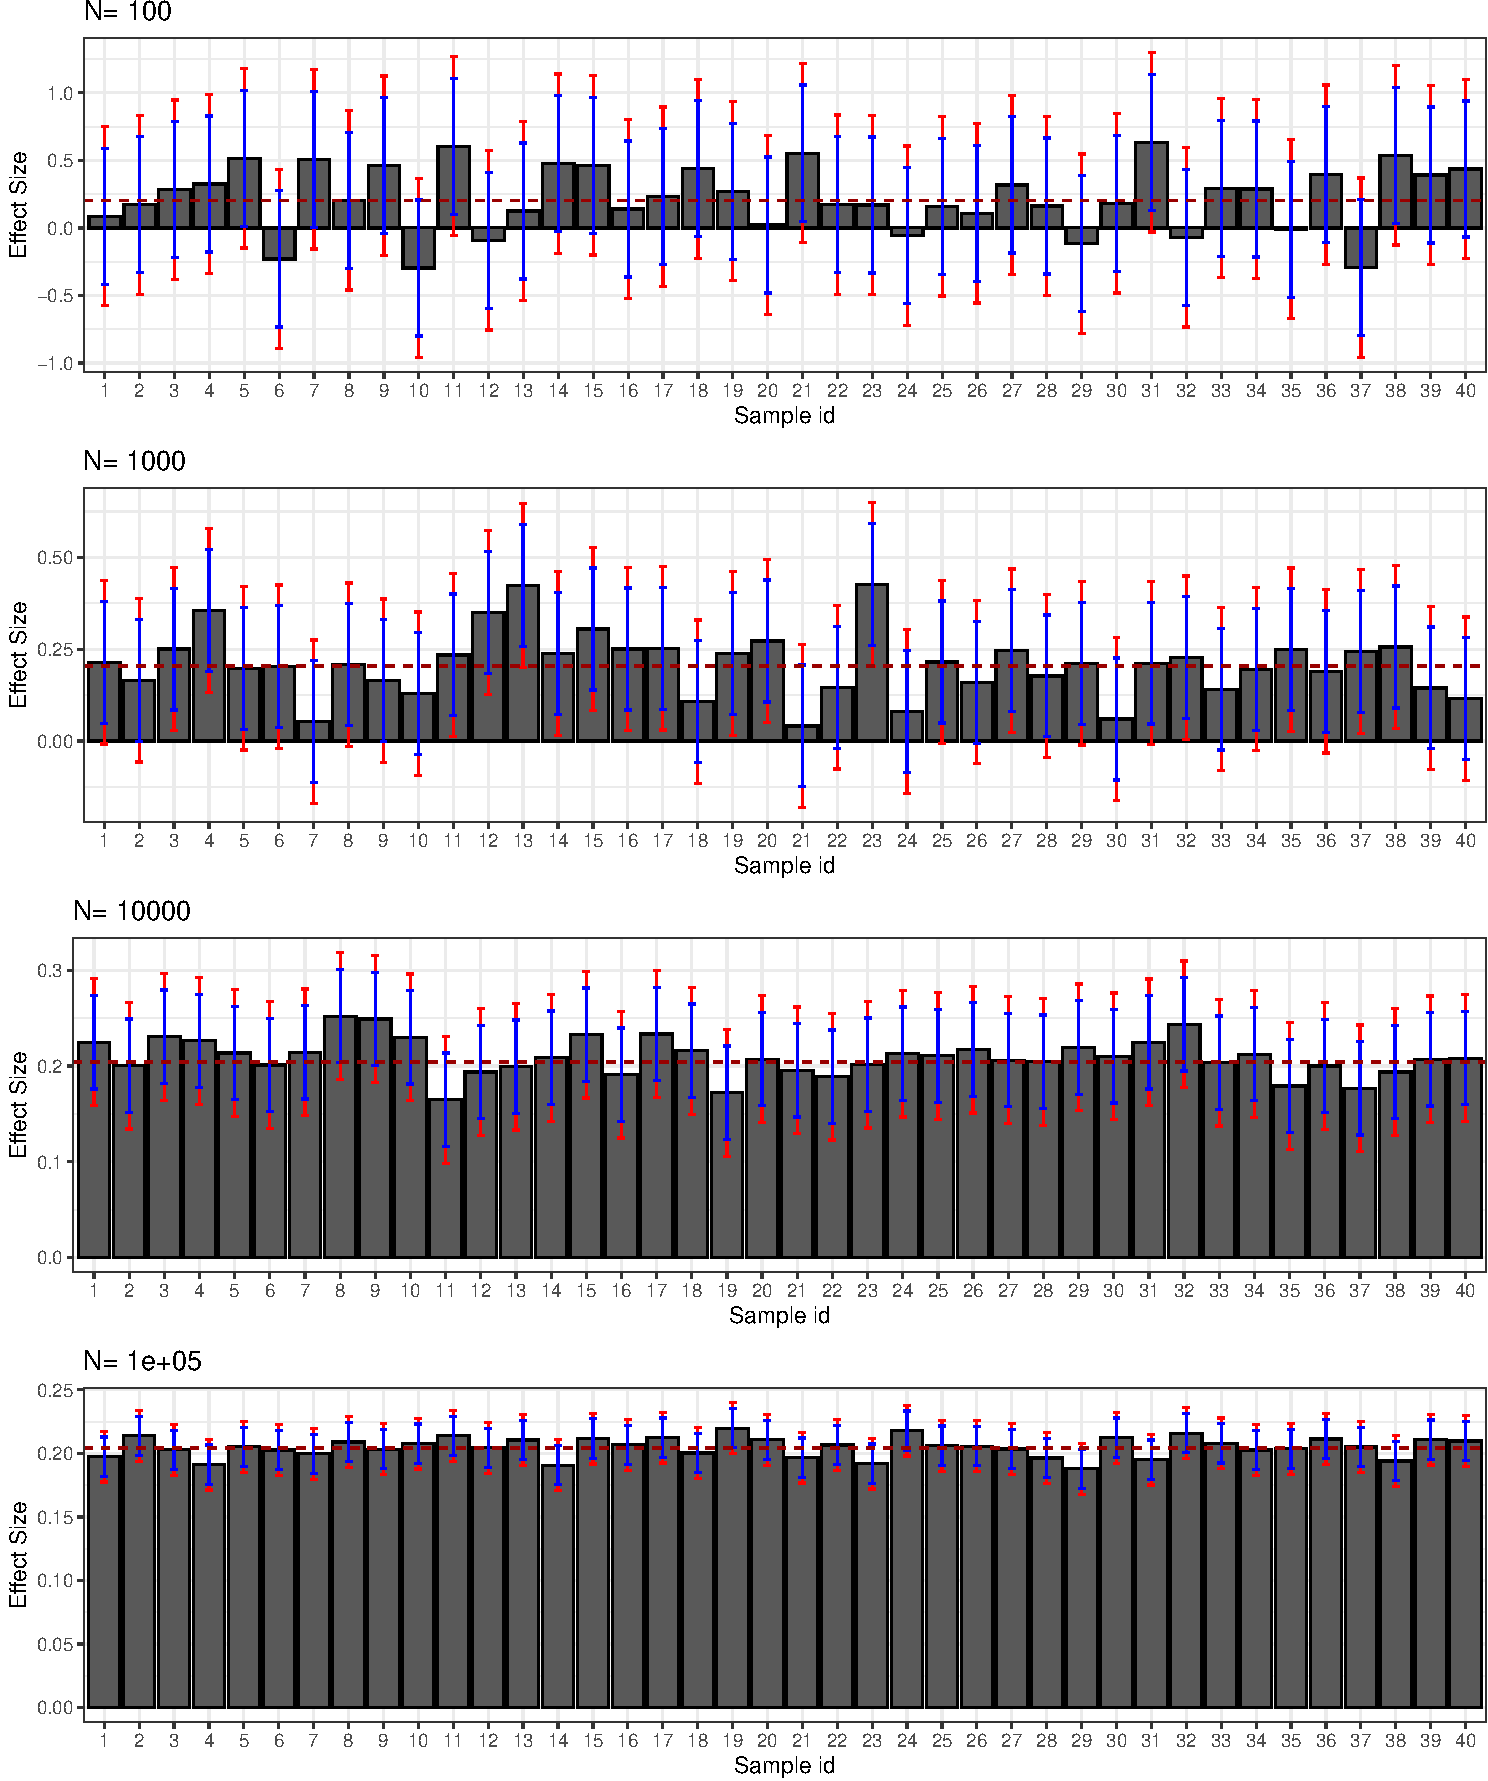
\includegraphics[width=0.6\linewidth]{STCI_files/figure-latex/confintervalES-1} 

}

\caption{Confidence intervals of $\hat{ES}$ for $\delta=$ 0.99 (red) and 0.95 (blue) over sample replications for various sample sizes}\label{fig:confintervalES}
\end{figure}

Figure \ref{fig:confintervalES} presents the 99\% and 95\% confidence intervals for the effect size estimated in 40 samples selected from our simulations.
Let's regroup our estimate and see how we could present their results.

\begin{Shaded}
\begin{Highlighting}[]
\NormalTok{test.all.ES <-}\StringTok{ }\KeywordTok{list}\NormalTok{()}
\ControlFlowTok{for}\NormalTok{ (k }\ControlFlowTok{in} \DecValTok{1}\OperatorTok{:}\KeywordTok{length}\NormalTok{(N.sample))\{}
  \KeywordTok{set.seed}\NormalTok{(}\DecValTok{1234}\NormalTok{)}
\NormalTok{  test.ES <-}\StringTok{ }\KeywordTok{sample}\NormalTok{(simuls.ww[[k]][,}\StringTok{'ES'}\NormalTok{],N.plot)}
\NormalTok{  test.ES <-}\StringTok{ }\KeywordTok{as.data.frame}\NormalTok{(}\KeywordTok{cbind}\NormalTok{(test.ES,}\KeywordTok{rep}\NormalTok{(}\KeywordTok{samp.noise.ES}\NormalTok{(simuls.ww[[k]][,}\StringTok{'ES'}\NormalTok{],}\DataTypeTok{delta=}\NormalTok{delta,}\DataTypeTok{param=}\NormalTok{param)),}\KeywordTok{rep}\NormalTok{(}\KeywordTok{samp.noise.ES}\NormalTok{(simuls.ww[[k]][,}\StringTok{'ES'}\NormalTok{],}\DataTypeTok{delta=}\NormalTok{delta}\FloatTok{.2}\NormalTok{,}\DataTypeTok{param=}\NormalTok{param))))}
  \KeywordTok{colnames}\NormalTok{(test.ES) <-}\StringTok{ }\KeywordTok{c}\NormalTok{(}\StringTok{'ES'}\NormalTok{,}\StringTok{'sampling.noise.ES.1'}\NormalTok{,}\StringTok{'sampling.noise.ES.2'}\NormalTok{)}
\NormalTok{  test.ES}\OperatorTok{$}\NormalTok{id <-}\StringTok{ }\DecValTok{1}\OperatorTok{:}\NormalTok{N.plot.ES}
\NormalTok{  test.all.ES[[k]] <-}\StringTok{ }\NormalTok{test.ES}
\NormalTok{\}}
\end{Highlighting}
\end{Shaded}

With \(N=\) 100, the reporting of the results for sample 1 would be something like: ``we find an effect size of 0.09 \(\pm\) 0.66'' with \(\delta=0,99\).
With \(\delta=0.95\) we would say: ``we find an effect of 0.09 \(\pm\) 0.5.''
All in all, our estimate is compatible with the treatment having a large positive effect size and a medium negative effect size.
Low precision prevents us from saying much else.

With \(N=\) 1000, the reporting of the results for sample 1 with \(\delta=0.99\) would be something like: ``we find an effect size of 0.21 \(\pm\) 0.22.''
With \(\delta=0.95\): ``we find an effect size of 0.21 \(\pm\) 0.17.''
Our estimate is compatible with a medium positive effect or a very small positive or even negative effect (depending on the choice of \(\delta\)).

With \(N=\) \ensuremath{10^{4}}, the reporting of the results for sample 1 with \(\delta=0.99\) would be something like: ``we find an effect size of 0.22 \(\pm\) 0.07.''
With \(\delta=0.95\): ``we find an effect size of 0.22 \(\pm\) 0.05.''
Our estimate is thus compatible with a small effect of the treatment.
We can rule out that the effect of the treatment is medium since the upper bound of the 99\% confidence interval is equal to 0.29.
We can also rule out that the effect of the treatment is very small since the lower bound of the 99\% confidence interval is equal to 0.16.
With this sample size, we have been able to reach a precision level sufficient enough to pin down the order of magnitude of the effect size of our treatment.
There still remains a considerable amount of uncertainty about the true effect size, though: the upper bound of our confidence interval is almost double the lower bound.

With \(N=\) \ensuremath{10^{5}}, the reporting of the results for sample 1 with \(\delta=0.99\) would be something like: ``we find an effect size of 0.2 \(\pm\) 0.02.''
With \(\delta=0.95\): ``we find an effect size of 0.2 \(\pm\) 0.02.''
Here, the level of precision of our result is such that, first, it does not depend on the choice of \(\delta\) in any meaningful way, and second, we can do more than pinpoint the order of magnitude of the effect size, we can start to zero in on its precise value.
From our estimate, the true value of the effect size is really close to 0.2.
It could be equal to 0.18 or 0.22, but not further away from 0.2 than that.
Remember that is actually equal to 0.2.

\BeginKnitrBlock{remark}
\iffalse{} {Remark. } \fi{}One issue with Cohen's \(d\) is that its magnitude depends on the dispersion of the outcomes in the control group.
That means that for the same treatment, and same value of the treatment effect, the effect size is larger in a population where oucomes are more homogeneous.
This is not an attractive feature of a normalizing scale that its size depends on the particular application.
One solution would be, for each outcome, to provide a standardized scale, using for example the estmated standard deviation in a reference population.
This would be similar to the invention of the metric system, where a reference scale was agreed uppon once and for all.
\EndKnitrBlock{remark}

\BeginKnitrBlock{remark}
\iffalse{} {Remark. } \fi{}Cohen's \(d\) is well defined for continuous outcomes.
For discrete outcomes, the use of Cohen's \(d\) poses a series of problems, and alternatives such as relative risk ratios and odds ratios have been proposed.
I'll comment on that in the last chapter.
\EndKnitrBlock{remark}

\hypertarget{sec:estimsampnoise}{%
\section{Estimating sampling noise}\label{sec:estimsampnoise}}

Gauging the extent sampling noise is very useful in order to be able to determine how much we should trust our results.
Are they precise, so that the true treatment effect lies very close to our estimate?
Or are our results imprecise, the true treatment effect maybe lying very far from our estimate?

Estimating sampling noise is hard because we want to infer a property of our estimator over repeated samples using only one sample.
In this lecture, I am going to introduce four tools that enable you to gauge sampling noise and to choose sample size.
The four tools are Chebyshev's inequality, the Central Limit Theorem, resampling methods and Fisher's permutation method.
The idea of all these methods is to use the properties of the sample to infer the properties of our estimator over replications.
Chebyshev's inequality gives an upper bound on the sampling noise and a lower bound on sample size, but these bounds are generally too wide to be useful.
The Central Limit Theorem (CLT) approximates the distribution of \(\hat{E}\) by a normal distribution, and quantifies sampling noise as a multiple of the standard deviation.
Resampling methods use the sample as a population and draw new samples from it in order to approximate sampling noise.
Fisher's permutation method, also called randomization inference, derives the distribution of \(\hat{E}\) under the assumption that all treatment effects are null, by reallocating the treatment indicator among the treatment and control group.
Both the CLT and resampling methods are approximation methods, and their approximation of the true extent of sampling noise gets better and better as sample size increases.
Fisher's permutation method is exact-it is not an approximation-but it only works for the special case of the \(WW\) estimator in a randomized design.

The remaining of this section is structured as follows.
Section \ref{sec:assumptions} introduces the assumptions that we will need in order to implement the methods.
Section \ref{sec:cheb} presents the Chebyshev approach to gauging sampling noise and choosing sample size.
Section \ref{sec:CLT} introduces the CLT way of approximating sampling noise and choosing sample size.
Section \ref{sec:resamp} presents the resampling methods.
Section \ref{sec:Fisher} introduces the Fisher's exact permutation approach.

\BeginKnitrBlock{remark}
\iffalse{} {Remark. } \fi{}I am going to derive the estimators for the precision only for the \(WW\) estimator.
In the following lectures, I will show how these methods adapt to other estimators.
\EndKnitrBlock{remark}

\hypertarget{sec:assumptions}{%
\subsection{Assumptions}\label{sec:assumptions}}

In order to be able to use the theorems that power up the methods that we are going to use to gauge sampling noise, we need to make some assumptions on the properties of the data.
The main assumptions that we need are that the estimator identifies the true effect of the treatment in the population, that the estimator is well-defined in the sample, that the observations in the sample are independently and identically distributed (i.i.d.), that there is no interaction between units and that the variances of the outcomes in the treated and untreated group are finite.

We know from last lecture that for the \(WW\) estimator to identify \(TT\), we need to assume that there is no selection bias, as stated in Assumption \ref{def:noselb}.
One way to ensure that this assumption holds is to use a RCT.

In order to be able to form the \(WW\) estimator in the sample, we also need that there is at least one treated and one untreated in the sample:

\BeginKnitrBlock{definition}[Full rank]
\protect\hypertarget{def:fullrank}{}{\label{def:fullrank} \iffalse (Full rank) \fi{} }We assume that there is at least one observation in the sample that receives the treatment and one observation that does not receive it:
\begin{align*}
\exists i,j\leq N \text{ such that } & D_i=1 \& D_j=0.
\end{align*}
\EndKnitrBlock{definition}

One way to ensure that this assumption holds is to sample treated and untreated units.

In order to be able to estimate the variance of the estimator easily, we assume that the observations come from random sampling and are i.i.d.:

\BeginKnitrBlock{definition}[i.i.d. sampling]
\protect\hypertarget{def:iid}{}{\label{def:iid} \iffalse (i.i.d. sampling) \fi{} }We assume that the observations in the sample are identically and independently distributed:
\begin{align*}
\forall i,j\leq N\text{, }i\neq j\text{, } & (Y_i,D_i)\Ind(Y_j,D_j),\\
                                           & (Y_i,D_i)\&(Y_j,D_j)\sim F_{Y,D}.
\end{align*}
\EndKnitrBlock{definition}

We have to assume something on how the observations are related to each other and to the population.
Identical sampling is natural in the sense that we are OK to assume that the observations stem from the same population model.
Independent sampling is something else altogether.
Independence means that the fates of two closely related individuals are assumed to be independent.
This rules out two empirically relevant scenarios:

\begin{enumerate}
\def\labelenumi{\arabic{enumi}.}
\tightlist
\item
  The fates of individuals are related because of common influences, as for example the environment, etc,
\item
  The fates of individuals are related because they directly influence each other, as for example on a market, but also for example because there are diffusion effects, such as contagion of deseases or technological adoption by imitation.
\end{enumerate}

We will address both sources of failure of the independence assumption in future lectures.

Finally, in order for all our derivations to make sense, we need to assume that the outcomes in both groups have finite variances, otherwise sampling noise is going to be too extreme to be able to estimate it using the methods developed in this lecture:

\BeginKnitrBlock{definition}[Finite variance of $\hat{\Delta^Y_{WW}}$]
\protect\hypertarget{def:finitevar}{}{\label{def:finitevar} \iffalse (Finite variance of \(\hat{\Delta^Y_{WW}}\)) \fi{} }We assume that \(\var{Y^1|D_i=1}\) and \(\var{Y^0|D_i=0}\) are finite.
\EndKnitrBlock{definition}

\hypertarget{sec:cheb}{%
\subsection{Using Chebyshev's inequality}\label{sec:cheb}}

Chebyshev's inequality is a fundamental building block of statistics.
It relates the sampling noise of an estimator to its variance.
More precisely, it derives an upper bound on the samplig noise of an unbiased estimator:

\BeginKnitrBlock{theorem}[Chebyshev's inequality]
\protect\hypertarget{thm:cheb}{}{\label{thm:cheb} \iffalse (Chebyshev's inequality) \fi{} }For any unbiased estimator \(\hat{\theta}\), sampling noise level \(2\epsilon\) and confidence level \(\delta\), sampling noise is bounded from above:

\begin{align*}
2\epsilon \leq 2\sqrt{\frac{\var{\hat{\theta}}}{1-\delta}}.
\end{align*}
\EndKnitrBlock{theorem}

\BeginKnitrBlock{remark}
\iffalse{} {Remark. } \fi{}The more general version of Chebyshev's inequality that is generally presented is as follows:

\begin{align*}
\Pr(|\hat{\theta}-\esp{\hat{\theta}}|>\epsilon) & \leq \frac{\var{\hat{\theta}}}{\epsilon^2}.
\end{align*}

The version I present in Theorem \ref{thm:cheb} is adapted to the bouding of sampling noise for a given confidence level, while this version is adapted to bounding the confidence level for a given level of sampling noise.
In order to go from this general version to Theorem \ref{thm:cheb}, simply remember that, for an unbiased estimator, \(\esp{\hat{\theta}}=\theta\) and that, by definition of sampling noise, \(\Pr(|\hat{\theta}-\theta|>\epsilon)=1-\delta\).
As a result, \(1-\delta\leq\var{\hat{\theta}}/\epsilon^2\), hence the result in Theorem \ref{thm:cheb}.
\EndKnitrBlock{remark}

Using Chebyshev's inequality, we can obtain an upper bound on the sampling noise of the \(WW\) estimator:

\BeginKnitrBlock{theorem}[Upper bound on the sampling noise of $\hat{WW}$]
\protect\hypertarget{thm:uppsampnoise}{}{\label{thm:uppsampnoise} \iffalse (Upper bound on the sampling noise of \(\hat{WW}\)) \fi{} }Under Assumptions \ref{def:noselb}, \ref{def:fullrank} and \ref{def:iid}, for a given confidence level \(\delta\), the sampling noise of the \(\hat{WW}\) estimator is bounded from above:

\begin{align*}
2\epsilon \leq 2\sqrt{\frac{1}{N(1-\delta)}\left(\frac{\var{Y_i^1|D_i=1}}{\Pr(D_i=1)}+\frac{\var{Y_i^0|D_i=0}}{1-\Pr(D_i=1)}\right)}\equiv 2\bar{\epsilon}.
\end{align*}
\EndKnitrBlock{theorem}

\BeginKnitrBlock{proof}
\iffalse{} {Proof. } \fi{}See in Appendix \ref{proofcheb}
\EndKnitrBlock{proof}

Theorem \ref{thm:uppsampnoise} is a useful step forward for estimating sampling noise.
Theorem \ref{thm:uppsampnoise} states that the actual level of sampling noise of the \(\hat{WW}\) estimator (\(2\epsilon\)) is never bigger than a quantity that depends on sample size, confidence level and on the variances of outcomes in the treated and control groups.
We either know all the components of the formula for \(2\bar{\epsilon}\) or we can estimate them in the sample.
For example, \(\Pr(D_i=1)\), \(\var{Y_i^1|D_i=1}\) and \(\var{Y_i^0|D_i=0}\) by can be approximated by, respectively:

\begin{align*}
  \hat{\Pr(D_i=1)} & = \frac{1}{N}\sum_{i=1}^ND_i\\
  \hat{\var{Y_i^1|D_i=1}} & = \frac{1}{\sum_{i=1}^ND_i}\sum_{i=1}^ND_i(Y_i-\frac{1}{\sum_{i=1}^ND_i}\sum_{i=1}^ND_iY_i)^2\\
  \hat{\var{Y_i^0|D_i=0}} & = \frac{1}{\sum_{i=1}^N(1-D_i)}\sum_{i=1}^N(1-D_i)(Y_i-\frac{1}{\sum_{i=1}^N(1-D_i)}\sum_{i=1}^N(1-D_i)Y_i)^2.
\end{align*}

Using these approximations for the quantities in the formula, we can compute an estimate of the upper bound on sampling noise, \(\hat{2\bar{\epsilon}}\).

\BeginKnitrBlock{example}
\protect\hypertarget{exm:unnamed-chunk-47}{}{\label{exm:unnamed-chunk-47} }Let's write an R function that is going to compute an estimate for the upper bound of sampling noise for any sample:
\EndKnitrBlock{example}

\begin{Shaded}
\begin{Highlighting}[]
\NormalTok{samp.noise.ww.cheb <-}\StringTok{ }\ControlFlowTok{function}\NormalTok{(N,delta,v1,v0,p)\{}
  \KeywordTok{return}\NormalTok{(}\DecValTok{2}\OperatorTok{*}\KeywordTok{sqrt}\NormalTok{((v1}\OperatorTok{/}\NormalTok{p}\OperatorTok{+}\NormalTok{v0}\OperatorTok{/}\NormalTok{(}\DecValTok{1}\OperatorTok{-}\NormalTok{p))}\OperatorTok{/}\NormalTok{(N}\OperatorTok{*}\NormalTok{(}\DecValTok{1}\OperatorTok{-}\NormalTok{delta))))}
\NormalTok{\}}
\end{Highlighting}
\end{Shaded}

Let's estimate this upper bound in our usual sample:

\begin{Shaded}
\begin{Highlighting}[]
\KeywordTok{set.seed}\NormalTok{(}\DecValTok{1234}\NormalTok{)}
\NormalTok{N <-}\DecValTok{1000}
\NormalTok{delta <-}\StringTok{ }\FloatTok{0.99}
\NormalTok{mu <-}\StringTok{ }\KeywordTok{rnorm}\NormalTok{(N,param[}\StringTok{"barmu"}\NormalTok{],}\KeywordTok{sqrt}\NormalTok{(param[}\StringTok{"sigma2mu"}\NormalTok{]))}
\NormalTok{UB <-}\StringTok{ }\KeywordTok{rnorm}\NormalTok{(N,}\DecValTok{0}\NormalTok{,}\KeywordTok{sqrt}\NormalTok{(param[}\StringTok{"sigma2U"}\NormalTok{]))}
\NormalTok{yB <-}\StringTok{ }\NormalTok{mu }\OperatorTok{+}\StringTok{ }\NormalTok{UB }
\NormalTok{YB <-}\StringTok{ }\KeywordTok{exp}\NormalTok{(yB)}
\NormalTok{Ds <-}\StringTok{ }\KeywordTok{rep}\NormalTok{(}\DecValTok{0}\NormalTok{,N)}
\NormalTok{V <-}\StringTok{ }\KeywordTok{rnorm}\NormalTok{(N,param[}\StringTok{"barmu"}\NormalTok{],}\KeywordTok{sqrt}\NormalTok{(param[}\StringTok{"sigma2mu"}\NormalTok{]}\OperatorTok{+}\NormalTok{param[}\StringTok{"sigma2U"}\NormalTok{]))}
\NormalTok{Ds[V}\OperatorTok{<=}\KeywordTok{log}\NormalTok{(param[}\StringTok{"barY"}\NormalTok{])] <-}\StringTok{ }\DecValTok{1} 
\NormalTok{epsilon <-}\StringTok{ }\KeywordTok{rnorm}\NormalTok{(N,}\DecValTok{0}\NormalTok{,}\KeywordTok{sqrt}\NormalTok{(param[}\StringTok{"sigma2epsilon"}\NormalTok{]))}
\NormalTok{eta<-}\StringTok{ }\KeywordTok{rnorm}\NormalTok{(N,}\DecValTok{0}\NormalTok{,}\KeywordTok{sqrt}\NormalTok{(param[}\StringTok{"sigma2eta"}\NormalTok{]))}
\NormalTok{U0 <-}\StringTok{ }\NormalTok{param[}\StringTok{"rho"}\NormalTok{]}\OperatorTok{*}\NormalTok{UB }\OperatorTok{+}\StringTok{ }\NormalTok{epsilon}
\NormalTok{y0 <-}\StringTok{ }\NormalTok{mu }\OperatorTok{+}\StringTok{  }\NormalTok{U0 }\OperatorTok{+}\StringTok{ }\NormalTok{param[}\StringTok{"delta"}\NormalTok{]}
\NormalTok{alpha <-}\StringTok{ }\NormalTok{param[}\StringTok{"baralpha"}\NormalTok{]}\OperatorTok{+}\StringTok{  }\NormalTok{param[}\StringTok{"theta"}\NormalTok{]}\OperatorTok{*}\NormalTok{mu }\OperatorTok{+}\StringTok{ }\NormalTok{eta}
\NormalTok{y1 <-}\StringTok{ }\NormalTok{y0}\OperatorTok{+}\NormalTok{alpha}
\NormalTok{Y0 <-}\StringTok{ }\KeywordTok{exp}\NormalTok{(y0)}
\NormalTok{Y1 <-}\StringTok{ }\KeywordTok{exp}\NormalTok{(y1)}
\NormalTok{y <-}\StringTok{ }\NormalTok{y1}\OperatorTok{*}\NormalTok{Ds}\OperatorTok{+}\NormalTok{y0}\OperatorTok{*}\NormalTok{(}\DecValTok{1}\OperatorTok{-}\NormalTok{Ds)}
\NormalTok{Y <-}\StringTok{ }\NormalTok{Y1}\OperatorTok{*}\NormalTok{Ds}\OperatorTok{+}\NormalTok{Y0}\OperatorTok{*}\NormalTok{(}\DecValTok{1}\OperatorTok{-}\NormalTok{Ds)}
\end{Highlighting}
\end{Shaded}

In our sample, for \(\delta=\) 0.99, \(\hat{2\bar{\epsilon}}=\) 1.35.
How does this compare with the true extent of sampling noise when \(N=\) 1000?
Remember that we have computed an estimate of sampling noise out of our Monte Carlo replications.
In Table \ref{fig:precision}, we can read that sampling noise is actually equal to 0.39.
The Chebyshev upper bound overestimates the extent of sampling noise by 245\%.

How does the Chebyshev upper bound fares overall?
In order to know that, let's compute the Chebyshev upper bound for all the simulated samples.
You might have noticed that, when running the Monte Carlo simulations for the population parameter, I have not only recovered \(\hat{WW}\) for each sample, but also the estimates of the components of the formula for the upper bound on sampling noise.
I can thus easily compute the Chebyshev upper bound on sampling noise for each replication.

\begin{Shaded}
\begin{Highlighting}[]
\ControlFlowTok{for}\NormalTok{ (k }\ControlFlowTok{in}\NormalTok{ (}\DecValTok{1}\OperatorTok{:}\KeywordTok{length}\NormalTok{(N.sample)))\{}
\NormalTok{  simuls.ww[[k]]}\OperatorTok{$}\NormalTok{cheb.noise <-}\StringTok{ }\KeywordTok{samp.noise.ww.cheb}\NormalTok{(N.sample[[k]],delta,simuls.ww[[k]][,}\StringTok{'V1'}\NormalTok{],simuls.ww[[k]][,}\StringTok{'V0'}\NormalTok{],simuls.ww[[k]][,}\StringTok{'p'}\NormalTok{])}
\NormalTok{\}}
\KeywordTok{par}\NormalTok{(}\DataTypeTok{mfrow=}\KeywordTok{c}\NormalTok{(}\DecValTok{2}\NormalTok{,}\DecValTok{2}\NormalTok{))}
\ControlFlowTok{for}\NormalTok{ (i }\ControlFlowTok{in} \DecValTok{1}\OperatorTok{:}\DecValTok{4}\NormalTok{)\{}
  \KeywordTok{hist}\NormalTok{(simuls.ww[[i]][,}\StringTok{'cheb.noise'}\NormalTok{],}\DataTypeTok{main=}\KeywordTok{paste}\NormalTok{(}\StringTok{'N='}\NormalTok{,}\KeywordTok{as.character}\NormalTok{(N.sample[i])),}\DataTypeTok{xlab=}\KeywordTok{expression}\NormalTok{(}\KeywordTok{hat}\NormalTok{(}\DecValTok{2}\OperatorTok{*}\KeywordTok{bar}\NormalTok{(epsilon))),}\DataTypeTok{xlim=}\KeywordTok{c}\NormalTok{(}\FloatTok{0.25}\OperatorTok{*}\KeywordTok{min}\NormalTok{(simuls.ww[[i]][,}\StringTok{'cheb.noise'}\NormalTok{]),}\KeywordTok{max}\NormalTok{(simuls.ww[[i]][,}\StringTok{'cheb.noise'}\NormalTok{])))}
  \KeywordTok{abline}\NormalTok{(}\DataTypeTok{v=}\NormalTok{table.noise[i,}\KeywordTok{colnames}\NormalTok{(table.noise)}\OperatorTok{==}\StringTok{'sampling.noise'}\NormalTok{],}\DataTypeTok{col=}\StringTok{"red"}\NormalTok{)}
\NormalTok{\}}
\end{Highlighting}
\end{Shaded}

\begin{figure}[htbp]

{\centering 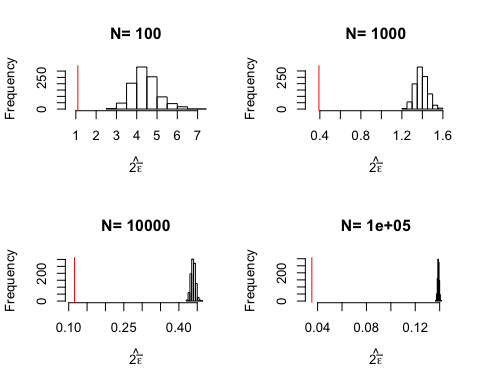
\includegraphics[width=0.6\linewidth]{STCI_files/figure-latex/sampnoisewwcheball-1} 

}

\caption{Distribution of the Chebyshev upper bound on sampling noise over replications of samples of different sizes (true sampling noise in red)}\label{fig:sampnoisewwcheball}
\end{figure}

Figure \ref{fig:sampnoisewwcheball} shows that the upper bound works: it is always bigger than the true sampling noise.
Figure \ref{fig:sampnoisewwcheball} also shows that the upper bound is large: it generally is of an order of magnitude bigger than the true sampling noise, and thus offers a blurry and too pessimistic view of the precision of an estimator.
Figure \ref{fig:sampnoisewwchebplot} shows that the average Chebyshev bound gives an inflated estimate of sampling noise.
Figure \ref{fig:confintervalcheb} shows that the Chebyshev confidence intervals are clearly less precise than the true unknown ones.
With \(N=\) 1000, the true confidence intervals generally reject large negative effects, whereas the Chebyshev confidence intervals do not rule out this possibility.
With \(N=\) \ensuremath{10^{4}}, the true confidence intervals generally reject effects smaller than 0.1, whereas the Chebyshev confidence intervals cannot rule out small negative effects.

As a conclusion on Chebyshev estimates of sampling noise, their advantage is that they offer an upper bound on the noise: we can never underestimate noise if we use them.
A downside of Chebyshev sampling noise estimates is their low precision, which makes it hard to pinpoint the true confidence intervals.

\begin{Shaded}
\begin{Highlighting}[]
\ControlFlowTok{for}\NormalTok{ (k }\ControlFlowTok{in}\NormalTok{ (}\DecValTok{1}\OperatorTok{:}\KeywordTok{length}\NormalTok{(N.sample)))\{}
\NormalTok{  table.noise}\OperatorTok{$}\NormalTok{cheb.noise[k] <-}\StringTok{ }\KeywordTok{mean}\NormalTok{(simuls.ww[[k]]}\OperatorTok{$}\NormalTok{cheb.noise)}
\NormalTok{\}}
\KeywordTok{ggplot}\NormalTok{(table.noise, }\KeywordTok{aes}\NormalTok{(}\DataTypeTok{x=}\KeywordTok{as.factor}\NormalTok{(N), }\DataTypeTok{y=}\NormalTok{TT)) }\OperatorTok{+}
\StringTok{  }\KeywordTok{geom_bar}\NormalTok{(}\DataTypeTok{position=}\KeywordTok{position_dodge}\NormalTok{(), }\DataTypeTok{stat=}\StringTok{"identity"}\NormalTok{, }\DataTypeTok{colour=}\StringTok{'black'}\NormalTok{) }\OperatorTok{+}
\StringTok{  }\KeywordTok{geom_errorbar}\NormalTok{(}\KeywordTok{aes}\NormalTok{(}\DataTypeTok{ymin=}\NormalTok{TT}\OperatorTok{-}\NormalTok{sampling.noise}\OperatorTok{/}\DecValTok{2}\NormalTok{, }\DataTypeTok{ymax=}\NormalTok{TT}\OperatorTok{+}\NormalTok{sampling.noise}\OperatorTok{/}\DecValTok{2}\NormalTok{), }\DataTypeTok{width=}\NormalTok{.}\DecValTok{2}\NormalTok{,}\DataTypeTok{position=}\KeywordTok{position_dodge}\NormalTok{(.}\DecValTok{9}\NormalTok{),}\DataTypeTok{color=}\StringTok{'red'}\NormalTok{) }\OperatorTok{+}
\StringTok{  }\KeywordTok{geom_errorbar}\NormalTok{(}\KeywordTok{aes}\NormalTok{(}\DataTypeTok{ymin=}\NormalTok{TT}\OperatorTok{-}\NormalTok{cheb.noise}\OperatorTok{/}\DecValTok{2}\NormalTok{, }\DataTypeTok{ymax=}\NormalTok{TT}\OperatorTok{+}\NormalTok{cheb.noise}\OperatorTok{/}\DecValTok{2}\NormalTok{), }\DataTypeTok{width=}\NormalTok{.}\DecValTok{2}\NormalTok{,}\DataTypeTok{position=}\KeywordTok{position_dodge}\NormalTok{(.}\DecValTok{9}\NormalTok{),}\DataTypeTok{color=}\StringTok{'blue'}\NormalTok{) }\OperatorTok{+}
\StringTok{  }\KeywordTok{xlab}\NormalTok{(}\StringTok{"Sample Size"}\NormalTok{)}\OperatorTok{+}
\StringTok{  }\KeywordTok{theme_bw}\NormalTok{()}
\end{Highlighting}
\end{Shaded}

\begin{figure}[htbp]

{\centering 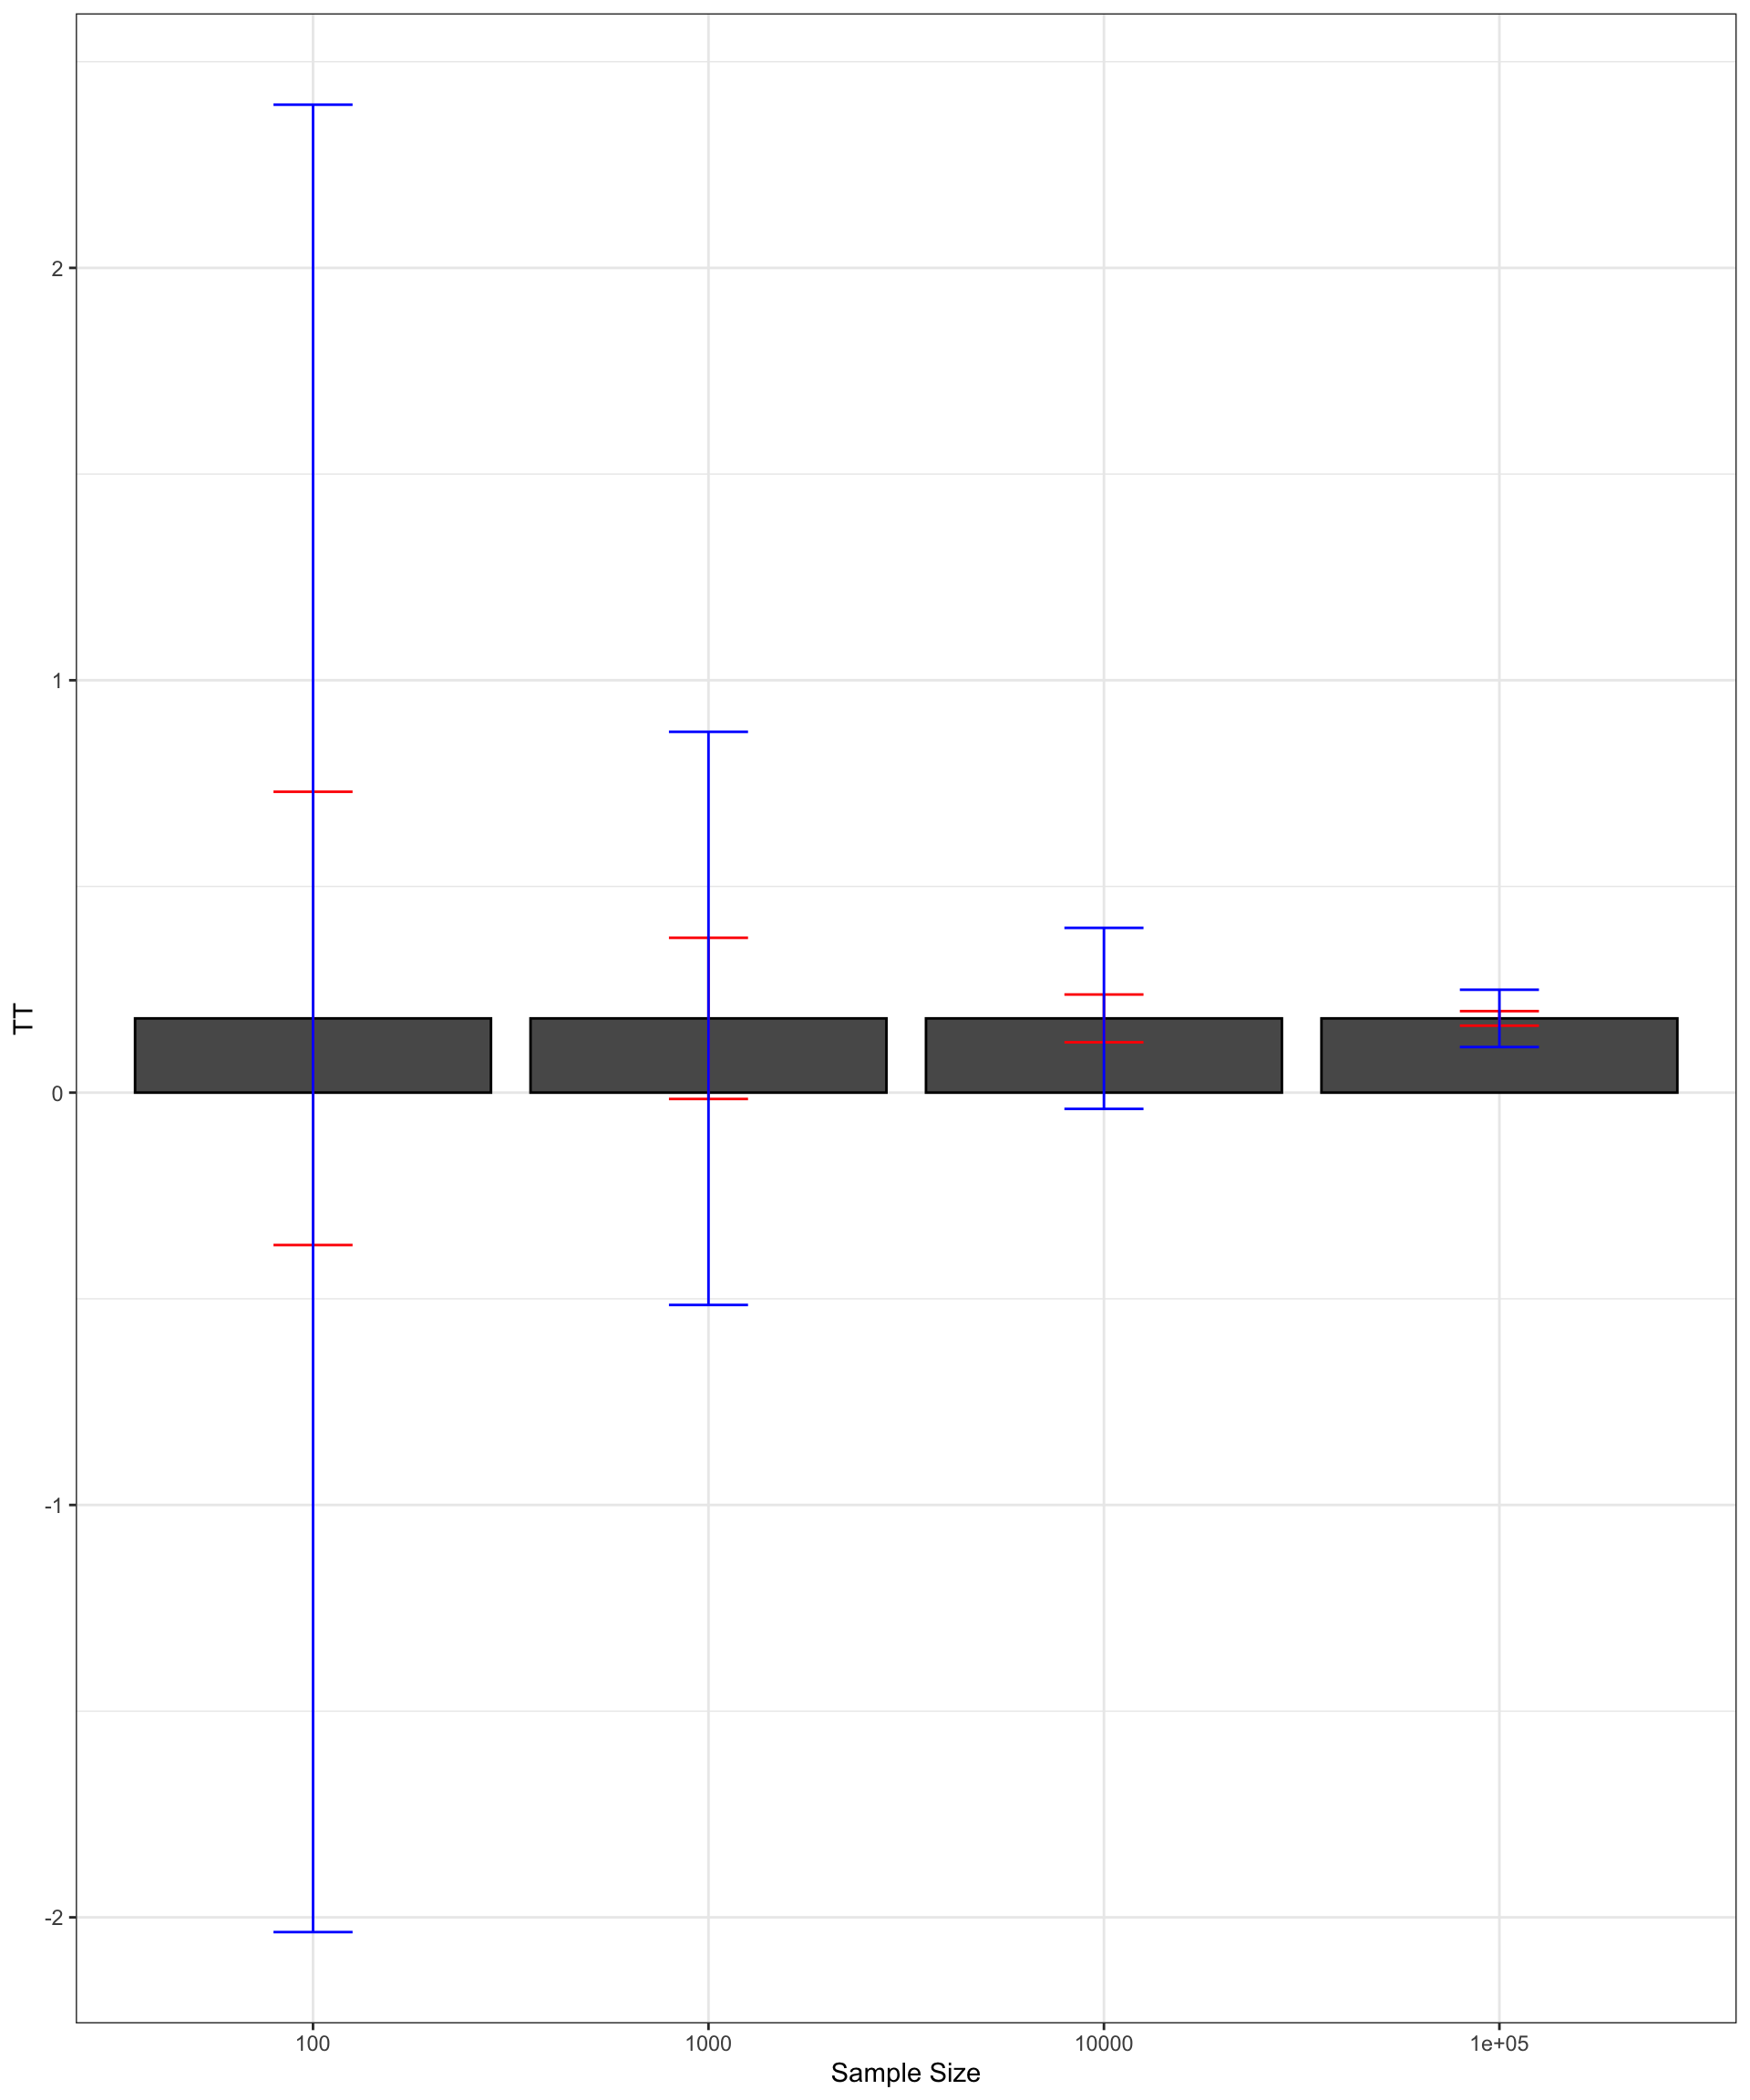
\includegraphics[width=0.6\linewidth]{STCI_files/figure-latex/sampnoisewwchebplot-1} 

}

\caption{Average Chebyshev upper bound on sampling noise over replications of samples of different sizes (true sampling noise in red)}\label{fig:sampnoisewwchebplot}
\end{figure}

\begin{Shaded}
\begin{Highlighting}[]
\NormalTok{N.plot <-}\StringTok{ }\DecValTok{40}
\NormalTok{plot.list <-}\StringTok{ }\KeywordTok{list}\NormalTok{()}

\ControlFlowTok{for}\NormalTok{ (k }\ControlFlowTok{in} \DecValTok{1}\OperatorTok{:}\KeywordTok{length}\NormalTok{(N.sample))\{}
  \KeywordTok{set.seed}\NormalTok{(}\DecValTok{1234}\NormalTok{)}
\NormalTok{  test.cheb <-}\StringTok{ }\NormalTok{simuls.ww[[k]][}\KeywordTok{sample}\NormalTok{(N.plot),}\KeywordTok{c}\NormalTok{(}\StringTok{'WW'}\NormalTok{,}\StringTok{'cheb.noise'}\NormalTok{)]}
\NormalTok{  test.cheb <-}\StringTok{ }\KeywordTok{as.data.frame}\NormalTok{(}\KeywordTok{cbind}\NormalTok{(test.cheb,}\KeywordTok{rep}\NormalTok{(}\KeywordTok{samp.noise}\NormalTok{(simuls.ww[[k]][,}\StringTok{'WW'}\NormalTok{],}\DataTypeTok{delta=}\NormalTok{delta),N.plot)))}
  \KeywordTok{colnames}\NormalTok{(test.cheb) <-}\StringTok{ }\KeywordTok{c}\NormalTok{(}\StringTok{'WW'}\NormalTok{,}\StringTok{'cheb.noise'}\NormalTok{,}\StringTok{'sampling.noise'}\NormalTok{)}
\NormalTok{  test.cheb}\OperatorTok{$}\NormalTok{id <-}\StringTok{ }\DecValTok{1}\OperatorTok{:}\NormalTok{N.plot}
\NormalTok{  plot.test.cheb <-}\StringTok{ }\KeywordTok{ggplot}\NormalTok{(test.cheb, }\KeywordTok{aes}\NormalTok{(}\DataTypeTok{x=}\KeywordTok{as.factor}\NormalTok{(id), }\DataTypeTok{y=}\NormalTok{WW)) }\OperatorTok{+}
\StringTok{      }\KeywordTok{geom_bar}\NormalTok{(}\DataTypeTok{position=}\KeywordTok{position_dodge}\NormalTok{(), }\DataTypeTok{stat=}\StringTok{"identity"}\NormalTok{, }\DataTypeTok{colour=}\StringTok{'black'}\NormalTok{) }\OperatorTok{+}
\StringTok{      }\KeywordTok{geom_errorbar}\NormalTok{(}\KeywordTok{aes}\NormalTok{(}\DataTypeTok{ymin=}\NormalTok{WW}\OperatorTok{-}\NormalTok{sampling.noise}\OperatorTok{/}\DecValTok{2}\NormalTok{, }\DataTypeTok{ymax=}\NormalTok{WW}\OperatorTok{+}\NormalTok{sampling.noise}\OperatorTok{/}\DecValTok{2}\NormalTok{), }\DataTypeTok{width=}\NormalTok{.}\DecValTok{2}\NormalTok{,}\DataTypeTok{position=}\KeywordTok{position_dodge}\NormalTok{(.}\DecValTok{9}\NormalTok{),}\DataTypeTok{color=}\StringTok{'red'}\NormalTok{) }\OperatorTok{+}
\StringTok{      }\KeywordTok{geom_errorbar}\NormalTok{(}\KeywordTok{aes}\NormalTok{(}\DataTypeTok{ymin=}\NormalTok{WW}\OperatorTok{-}\NormalTok{cheb.noise}\OperatorTok{/}\DecValTok{2}\NormalTok{, }\DataTypeTok{ymax=}\NormalTok{WW}\OperatorTok{+}\NormalTok{cheb.noise}\OperatorTok{/}\DecValTok{2}\NormalTok{), }\DataTypeTok{width=}\NormalTok{.}\DecValTok{2}\NormalTok{,}\DataTypeTok{position=}\KeywordTok{position_dodge}\NormalTok{(.}\DecValTok{9}\NormalTok{),}\DataTypeTok{color=}\StringTok{'blue'}\NormalTok{) }\OperatorTok{+}
\StringTok{      }\KeywordTok{geom_hline}\NormalTok{(}\KeywordTok{aes}\NormalTok{(}\DataTypeTok{yintercept=}\KeywordTok{delta.y.ate}\NormalTok{(param)), }\DataTypeTok{colour=}\StringTok{"#990000"}\NormalTok{, }\DataTypeTok{linetype=}\StringTok{"dashed"}\NormalTok{)}\OperatorTok{+}
\StringTok{      }\KeywordTok{xlab}\NormalTok{(}\StringTok{"Sample id"}\NormalTok{)}\OperatorTok{+}
\StringTok{      }\KeywordTok{theme_bw}\NormalTok{()}\OperatorTok{+}
\StringTok{      }\KeywordTok{ggtitle}\NormalTok{(}\KeywordTok{paste}\NormalTok{(}\StringTok{"N="}\NormalTok{,N.sample[k]))}
\NormalTok{  plot.list[[k]] <-}\StringTok{ }\NormalTok{plot.test.cheb }
\NormalTok{\}}
\NormalTok{plot.CI <-}\StringTok{ }\KeywordTok{plot_grid}\NormalTok{(plot.list[[}\DecValTok{1}\NormalTok{]],plot.list[[}\DecValTok{2}\NormalTok{]],plot.list[[}\DecValTok{3}\NormalTok{]],plot.list[[}\DecValTok{4}\NormalTok{]],}\DataTypeTok{ncol=}\DecValTok{1}\NormalTok{,}\DataTypeTok{nrow=}\KeywordTok{length}\NormalTok{(N.sample))}
\KeywordTok{print}\NormalTok{(plot.CI)}
\end{Highlighting}
\end{Shaded}

\begin{figure}[htbp]

{\centering 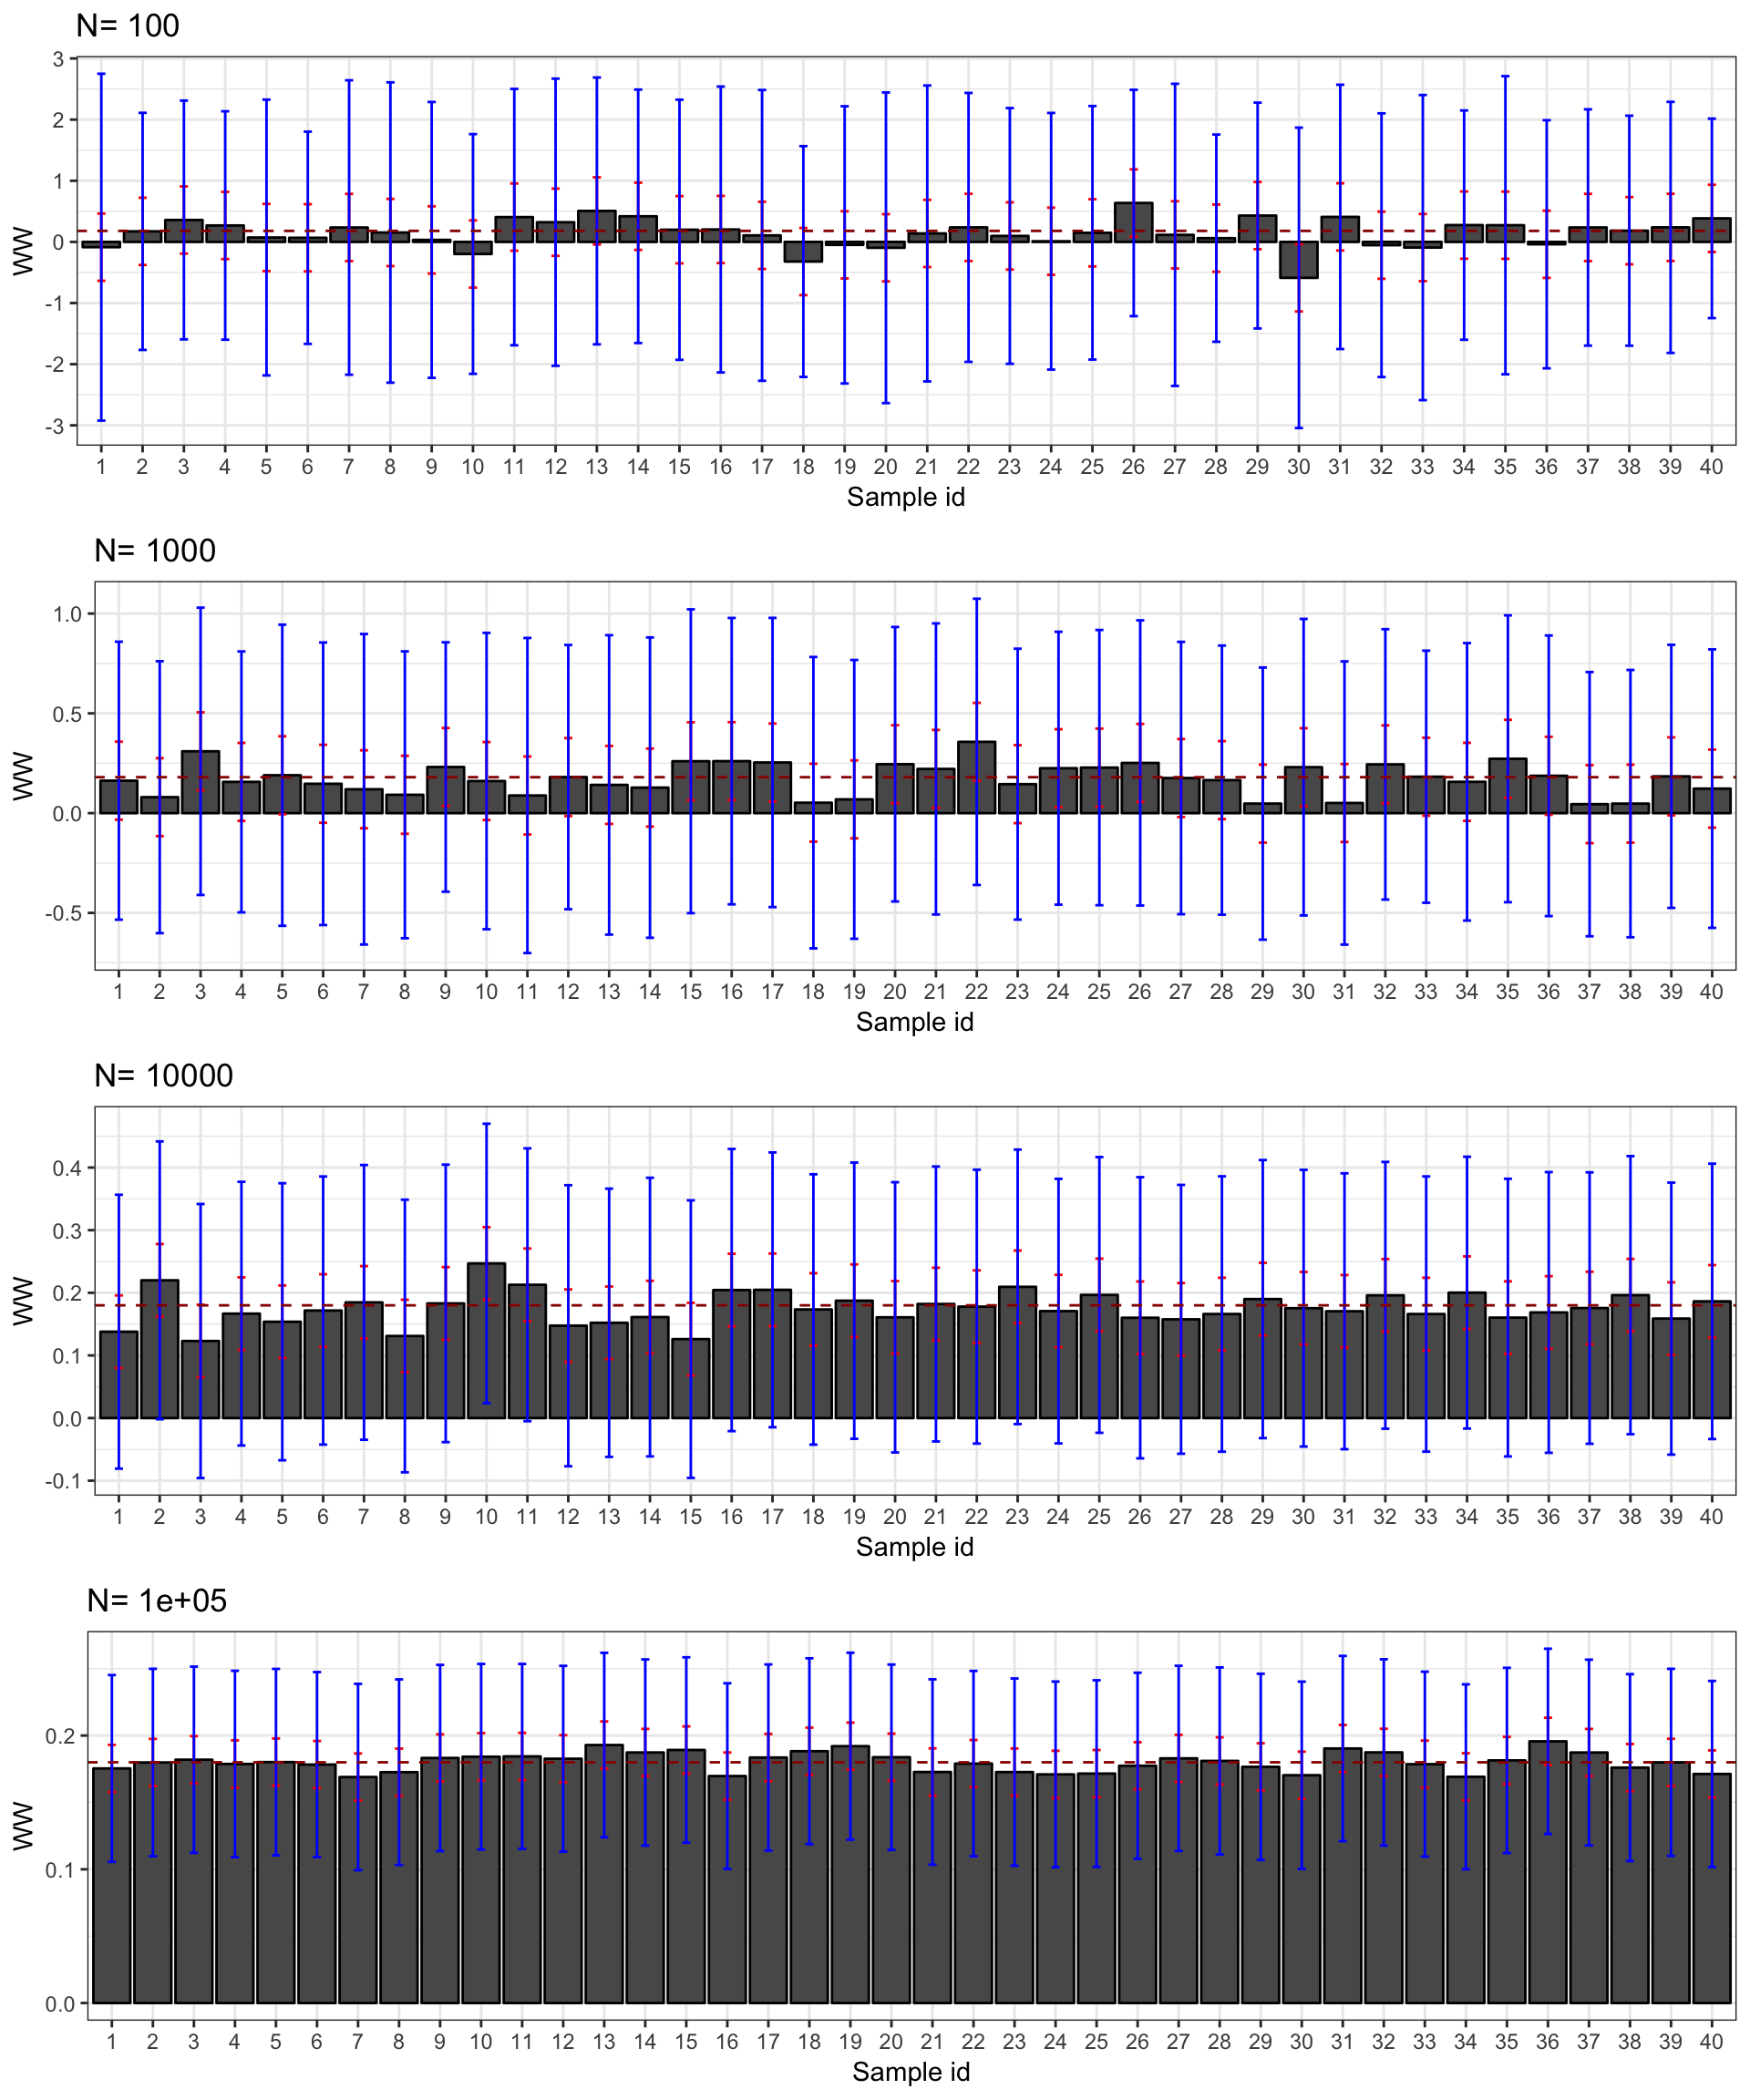
\includegraphics[width=0.6\linewidth]{STCI_files/figure-latex/confintervalcheb-1} 

}

\caption{Chebyshev confidence intervals of $\hat{WW}$ for $\delta=$ 0.99 over sample replications for various sample sizes (true confidence intervals in red)}\label{fig:confintervalcheb}
\end{figure}

\hypertarget{sec:CLT}{%
\subsection{Using the Central Limit Theorem}\label{sec:CLT}}

The main problem with Chebyshev's upper bound on sampling noise is that it is an upper bound, and thus it overestimates sampling noise and underestimates precision.
One alternative to using Chebyshev's upper bound is to use the Central Limit Theorem (CLT).
In econometrics and statistics, the CLT is used to derive approximate values for the sampling noise of estimators.
Because these approximations become more and more precise as sample size increases, we call them asymptotic approximations.

Taken to its bare bones, the CLT states that the sum of i.i.d. random variables behaves approximately like a normal distribution when the sample size is large:

\BeginKnitrBlock{theorem}[Central Limit Theorem]
\protect\hypertarget{thm:CLT}{}{\label{thm:CLT} \iffalse (Central Limit Theorem) \fi{} }Let \(X_i\) be i.i.d. random variables with \(\esp{X_i}=\mu\) and \(\var{X_i}=\sigma^2\), and define \(Z_N=\frac{\frac{1}{N}\sum_{i=1}^NX_i-\mu}{\frac{\sigma}{\sqrt{N}}}\), then, for all \(z\) we have:

\begin{align*}
\lim_{N\rightarrow\infty}\Pr(Z_N\leq z) & = \Phi(z),
\end{align*}
where \(\Phi\) is the cumulative distribution function of the centered standardized normal.

We say that \(Z_N\) converges in distribution to a standard normal random variable, and we denote: \(Z_N\stackrel{d}{\rightarrow}\mathcal{N}(0,1)\).
\EndKnitrBlock{theorem}

The CLT is a beautiful result: the distribution of the average of realisations of any random variable that has finite mean and variance can be approximated by a normal when the sample size is large enough.
The CLT is somehow limited though because not all estimators are sums.
Estimators are generally more or less complex combinations of sums.
In order to derive the asymptotic approximation for a lot of estimators that are combinations of sums, econometricians and statisticians complement the CLT with two other extremely powerful tools: Slutsky's theorem and the Delta method.
Slutsky's theorem states that sums, products and ratios of sums that converge to a normal converge to the sum, product or ratio of these normals.
The Delta method states that a function of a sum that converges to a normal converges to a normal whose variance is a quadratic form of the variance of the sum and of the first derivative of the function.
Both of these tools are stated more rigorously in the appendix, but you do not need to know them for this class.
The idea is for you to be aware of how the main approximations that we are going to use throughout this class have been derived.

Let me now state the main result of this section:

\BeginKnitrBlock{theorem}[Asymptotic Estimate of Sampling Noise of WW]
\protect\hypertarget{thm:asympnoiseWW}{}{\label{thm:asympnoiseWW} \iffalse (Asymptotic Estimate of Sampling Noise of WW) \fi{} }Under Assumptions \ref{def:noselb}, \ref{def:fullrank}, \ref{def:iid} and \ref{def:finitevar}, for a given confidence level \(\delta\) and sample size \(N\), the sampling noise of \(\hat{WW}\) can be approximated as follows:

\begin{align*}
2\epsilon & \approx 2\Phi^{-1}\left(\frac{\delta+1}{2}\right)\frac{1}{\sqrt{N}}\sqrt{\frac{\var{Y_i^1|D_i=1}}{\Pr(D_i=1)}+\frac{\var{Y_i^0|D_i=0}}{1-\Pr(D_i=1)}} \equiv 2\tilde{\epsilon}.
\end{align*}
\EndKnitrBlock{theorem}

\BeginKnitrBlock{proof}
\iffalse{} {Proof. } \fi{}See in Appendix \ref{proofCLT}.
\EndKnitrBlock{proof}

Let's write an R function that computes this formula:

\begin{Shaded}
\begin{Highlighting}[]
\NormalTok{samp.noise.ww.CLT <-}\StringTok{ }\ControlFlowTok{function}\NormalTok{(N,delta,v1,v0,p)\{}
  \KeywordTok{return}\NormalTok{(}\DecValTok{2}\OperatorTok{*}\KeywordTok{qnorm}\NormalTok{((delta}\OperatorTok{+}\DecValTok{1}\NormalTok{)}\OperatorTok{/}\DecValTok{2}\NormalTok{)}\OperatorTok{*}\KeywordTok{sqrt}\NormalTok{((v1}\OperatorTok{/}\NormalTok{p}\OperatorTok{+}\NormalTok{v0}\OperatorTok{/}\NormalTok{(}\DecValTok{1}\OperatorTok{-}\NormalTok{p))}\OperatorTok{/}\NormalTok{N))}
\NormalTok{\}}
\end{Highlighting}
\end{Shaded}

\BeginKnitrBlock{example}
\protect\hypertarget{exm:unnamed-chunk-49}{}{\label{exm:unnamed-chunk-49} }Let's see how the CLT performs in our example.
\EndKnitrBlock{example}

In our sample, for \(\delta=\) 0.99, the CLT estimate of sampling noise is \(\hat{2\tilde{\epsilon}}=\) 0.35.
How does this compare with the true extent of sampling noise when \(N=\) 1000?
Remember that we have computed an estimate of sampling noise out of our Monte Carlo replications.
In Table \ref{tab:precisionsignal}, we can read that sampling noise is actually equal to 0.39.
The CLT approximation is pretty precise: it only underestimates the true extent of sampling noise by 11\%.

We can also compute the CLT approximation to sampling noise in all of our samples:

\begin{Shaded}
\begin{Highlighting}[]
\ControlFlowTok{for}\NormalTok{ (k }\ControlFlowTok{in}\NormalTok{ (}\DecValTok{1}\OperatorTok{:}\KeywordTok{length}\NormalTok{(N.sample)))\{}
\NormalTok{  simuls.ww[[k]]}\OperatorTok{$}\NormalTok{CLT.noise <-}\StringTok{ }\KeywordTok{samp.noise.ww.CLT}\NormalTok{(N.sample[[k]],delta,simuls.ww[[k]][,}\StringTok{'V1'}\NormalTok{],simuls.ww[[k]][,}\StringTok{'V0'}\NormalTok{],simuls.ww[[k]][,}\StringTok{'p'}\NormalTok{])}
\NormalTok{\}}
\KeywordTok{par}\NormalTok{(}\DataTypeTok{mfrow=}\KeywordTok{c}\NormalTok{(}\DecValTok{2}\NormalTok{,}\DecValTok{2}\NormalTok{))}
\ControlFlowTok{for}\NormalTok{ (i }\ControlFlowTok{in} \DecValTok{1}\OperatorTok{:}\DecValTok{4}\NormalTok{)\{}
  \KeywordTok{hist}\NormalTok{(simuls.ww[[i]][,}\StringTok{'CLT.noise'}\NormalTok{],}\DataTypeTok{main=}\KeywordTok{paste}\NormalTok{(}\StringTok{'N='}\NormalTok{,}\KeywordTok{as.character}\NormalTok{(N.sample[i])),}\DataTypeTok{xlab=}\KeywordTok{expression}\NormalTok{(}\KeywordTok{hat}\NormalTok{(}\DecValTok{2}\OperatorTok{*}\KeywordTok{bar}\NormalTok{(epsilon))),}\DataTypeTok{xlim=}\KeywordTok{c}\NormalTok{(}\KeywordTok{min}\NormalTok{(simuls.ww[[i]][,}\StringTok{'CLT.noise'}\NormalTok{]),}\KeywordTok{max}\NormalTok{(simuls.ww[[i]][,}\StringTok{'CLT.noise'}\NormalTok{])))}
  \KeywordTok{abline}\NormalTok{(}\DataTypeTok{v=}\NormalTok{table.noise[i,}\KeywordTok{colnames}\NormalTok{(table.noise)}\OperatorTok{==}\StringTok{'sampling.noise'}\NormalTok{],}\DataTypeTok{col=}\StringTok{"red"}\NormalTok{)}
\NormalTok{\}}
\end{Highlighting}
\end{Shaded}

\begin{figure}[htbp]

{\centering 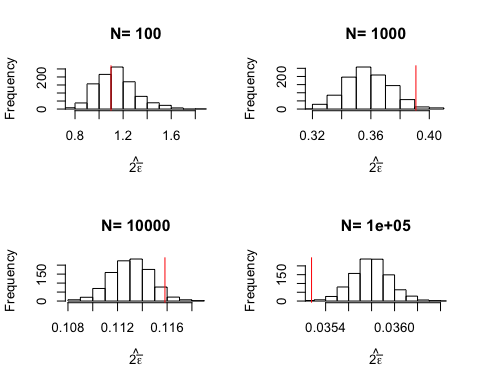
\includegraphics[width=0.6\linewidth]{STCI_files/figure-latex/sampnoisewwCLTall-1} 

}

\caption{Distribution of the CLT approximation of sampling noise over replications of samples of different sizes (true sampling noise in red)}\label{fig:sampnoisewwCLTall}
\end{figure}

Figure \ref{fig:sampnoisewwCLTall} shows that the CLT works: CLT-based estimates of sampling noise approximates true sampling noise well.
CLT-based approximations of sampling noise are even impressively accurate: they always capture the exact order of magnitude of sampling noise, although there is a slight underestimation when \(N=\) 1000 and \ensuremath{10^{4}} and a slight overestimation when \(N=\) \ensuremath{10^{5}}.
This success should not come as a surprise as all shocks in our model are normally distributed, meaning that the CLT results are more than an approximation, they are exact.
Results might be less spectacular when estimating the effect of the treatment on the outcomes in levels rather than in logs.

As a consequence, the average CLT-based estimates of sampling noise and of confidence intervals are pretty precise, as Figures \ref{fig:sampnoisewwCLTplot} and \ref{fig:confintervalCLT} show.
Let's pause for a second at the beauty of what we have achieved using the CLT: by using only information from one sample, we have been able to gauge extremely precisely how the estimator would behave over sampling repetitions.

\begin{Shaded}
\begin{Highlighting}[]
\ControlFlowTok{for}\NormalTok{ (k }\ControlFlowTok{in}\NormalTok{ (}\DecValTok{1}\OperatorTok{:}\KeywordTok{length}\NormalTok{(N.sample)))\{}
\NormalTok{  table.noise}\OperatorTok{$}\NormalTok{CLT.noise[k] <-}\StringTok{ }\KeywordTok{mean}\NormalTok{(simuls.ww[[k]]}\OperatorTok{$}\NormalTok{CLT.noise)}
\NormalTok{\}}
\KeywordTok{ggplot}\NormalTok{(table.noise, }\KeywordTok{aes}\NormalTok{(}\DataTypeTok{x=}\KeywordTok{as.factor}\NormalTok{(N), }\DataTypeTok{y=}\NormalTok{TT)) }\OperatorTok{+}
\StringTok{  }\KeywordTok{geom_bar}\NormalTok{(}\DataTypeTok{position=}\KeywordTok{position_dodge}\NormalTok{(), }\DataTypeTok{stat=}\StringTok{"identity"}\NormalTok{, }\DataTypeTok{colour=}\StringTok{'black'}\NormalTok{) }\OperatorTok{+}
\StringTok{  }\KeywordTok{geom_errorbar}\NormalTok{(}\KeywordTok{aes}\NormalTok{(}\DataTypeTok{ymin=}\NormalTok{TT}\OperatorTok{-}\NormalTok{sampling.noise}\OperatorTok{/}\DecValTok{2}\NormalTok{, }\DataTypeTok{ymax=}\NormalTok{TT}\OperatorTok{+}\NormalTok{sampling.noise}\OperatorTok{/}\DecValTok{2}\NormalTok{), }\DataTypeTok{width=}\NormalTok{.}\DecValTok{2}\NormalTok{,}\DataTypeTok{position=}\KeywordTok{position_dodge}\NormalTok{(.}\DecValTok{9}\NormalTok{),}\DataTypeTok{color=}\StringTok{'red'}\NormalTok{) }\OperatorTok{+}
\StringTok{  }\KeywordTok{geom_errorbar}\NormalTok{(}\KeywordTok{aes}\NormalTok{(}\DataTypeTok{ymin=}\NormalTok{TT}\OperatorTok{-}\NormalTok{CLT.noise}\OperatorTok{/}\DecValTok{2}\NormalTok{, }\DataTypeTok{ymax=}\NormalTok{TT}\OperatorTok{+}\NormalTok{CLT.noise}\OperatorTok{/}\DecValTok{2}\NormalTok{), }\DataTypeTok{width=}\NormalTok{.}\DecValTok{2}\NormalTok{,}\DataTypeTok{position=}\KeywordTok{position_dodge}\NormalTok{(.}\DecValTok{9}\NormalTok{),}\DataTypeTok{color=}\StringTok{'blue'}\NormalTok{) }\OperatorTok{+}
\StringTok{  }\KeywordTok{xlab}\NormalTok{(}\StringTok{"Sample Size"}\NormalTok{)}\OperatorTok{+}
\StringTok{  }\KeywordTok{theme_bw}\NormalTok{()}
\end{Highlighting}
\end{Shaded}

\begin{figure}[htbp]

{\centering 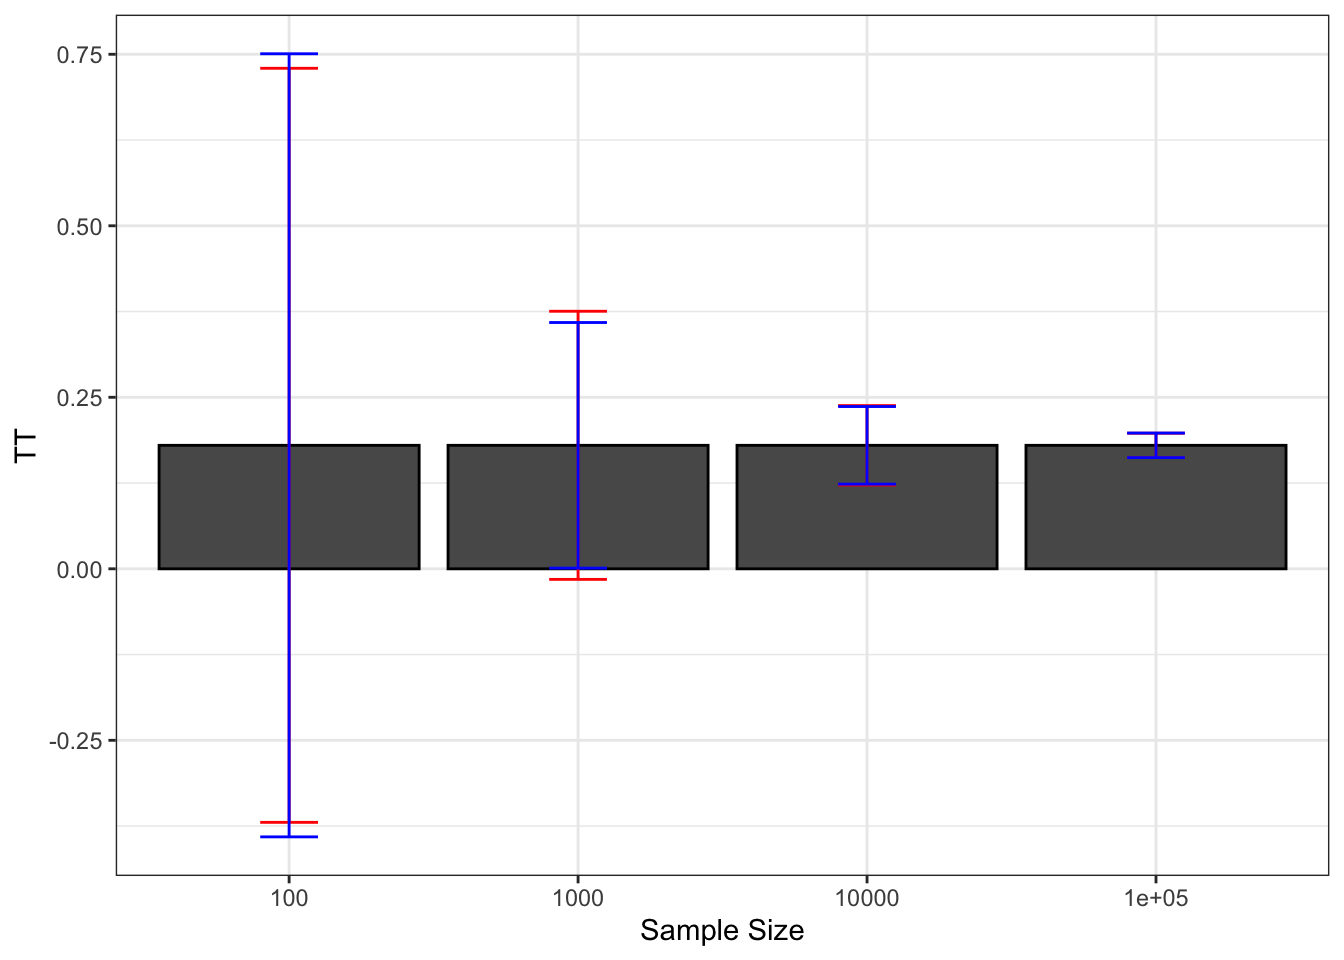
\includegraphics[width=0.6\linewidth]{STCI_files/figure-latex/sampnoisewwCLTplot-1} 

}

\caption{Average CLT-based approximations of sampling noise over replications of samples of different sizes (true sampling noise in red)}\label{fig:sampnoisewwCLTplot}
\end{figure}

\begin{Shaded}
\begin{Highlighting}[]
\NormalTok{N.plot <-}\StringTok{ }\DecValTok{40}
\NormalTok{plot.list <-}\StringTok{ }\KeywordTok{list}\NormalTok{()}

\ControlFlowTok{for}\NormalTok{ (k }\ControlFlowTok{in} \DecValTok{1}\OperatorTok{:}\KeywordTok{length}\NormalTok{(N.sample))\{}
  \KeywordTok{set.seed}\NormalTok{(}\DecValTok{1234}\NormalTok{)}
\NormalTok{  test.CLT <-}\StringTok{ }\NormalTok{simuls.ww[[k]][}\KeywordTok{sample}\NormalTok{(N.plot),}\KeywordTok{c}\NormalTok{(}\StringTok{'WW'}\NormalTok{,}\StringTok{'CLT.noise'}\NormalTok{)]}
\NormalTok{  test.CLT <-}\StringTok{ }\KeywordTok{as.data.frame}\NormalTok{(}\KeywordTok{cbind}\NormalTok{(test.CLT,}\KeywordTok{rep}\NormalTok{(}\KeywordTok{samp.noise}\NormalTok{(simuls.ww[[k]][,}\StringTok{'WW'}\NormalTok{],}\DataTypeTok{delta=}\NormalTok{delta),N.plot)))}
  \KeywordTok{colnames}\NormalTok{(test.CLT) <-}\StringTok{ }\KeywordTok{c}\NormalTok{(}\StringTok{'WW'}\NormalTok{,}\StringTok{'CLT.noise'}\NormalTok{,}\StringTok{'sampling.noise'}\NormalTok{)}
\NormalTok{  test.CLT}\OperatorTok{$}\NormalTok{id <-}\StringTok{ }\DecValTok{1}\OperatorTok{:}\NormalTok{N.plot}
\NormalTok{  plot.test.CLT <-}\StringTok{ }\KeywordTok{ggplot}\NormalTok{(test.CLT, }\KeywordTok{aes}\NormalTok{(}\DataTypeTok{x=}\KeywordTok{as.factor}\NormalTok{(id), }\DataTypeTok{y=}\NormalTok{WW)) }\OperatorTok{+}
\StringTok{      }\KeywordTok{geom_bar}\NormalTok{(}\DataTypeTok{position=}\KeywordTok{position_dodge}\NormalTok{(), }\DataTypeTok{stat=}\StringTok{"identity"}\NormalTok{, }\DataTypeTok{colour=}\StringTok{'black'}\NormalTok{) }\OperatorTok{+}
\StringTok{      }\KeywordTok{geom_errorbar}\NormalTok{(}\KeywordTok{aes}\NormalTok{(}\DataTypeTok{ymin=}\NormalTok{WW}\OperatorTok{-}\NormalTok{sampling.noise}\OperatorTok{/}\DecValTok{2}\NormalTok{, }\DataTypeTok{ymax=}\NormalTok{WW}\OperatorTok{+}\NormalTok{sampling.noise}\OperatorTok{/}\DecValTok{2}\NormalTok{), }\DataTypeTok{width=}\NormalTok{.}\DecValTok{2}\NormalTok{,}\DataTypeTok{position=}\KeywordTok{position_dodge}\NormalTok{(.}\DecValTok{9}\NormalTok{),}\DataTypeTok{color=}\StringTok{'red'}\NormalTok{) }\OperatorTok{+}
\StringTok{      }\KeywordTok{geom_errorbar}\NormalTok{(}\KeywordTok{aes}\NormalTok{(}\DataTypeTok{ymin=}\NormalTok{WW}\OperatorTok{-}\NormalTok{CLT.noise}\OperatorTok{/}\DecValTok{2}\NormalTok{, }\DataTypeTok{ymax=}\NormalTok{WW}\OperatorTok{+}\NormalTok{CLT.noise}\OperatorTok{/}\DecValTok{2}\NormalTok{), }\DataTypeTok{width=}\NormalTok{.}\DecValTok{2}\NormalTok{,}\DataTypeTok{position=}\KeywordTok{position_dodge}\NormalTok{(.}\DecValTok{9}\NormalTok{),}\DataTypeTok{color=}\StringTok{'blue'}\NormalTok{) }\OperatorTok{+}
\StringTok{      }\KeywordTok{geom_hline}\NormalTok{(}\KeywordTok{aes}\NormalTok{(}\DataTypeTok{yintercept=}\KeywordTok{delta.y.ate}\NormalTok{(param)), }\DataTypeTok{colour=}\StringTok{"#990000"}\NormalTok{, }\DataTypeTok{linetype=}\StringTok{"dashed"}\NormalTok{)}\OperatorTok{+}
\StringTok{      }\KeywordTok{xlab}\NormalTok{(}\StringTok{"Sample id"}\NormalTok{)}\OperatorTok{+}
\StringTok{      }\KeywordTok{theme_bw}\NormalTok{()}\OperatorTok{+}
\StringTok{      }\KeywordTok{ggtitle}\NormalTok{(}\KeywordTok{paste}\NormalTok{(}\StringTok{"N="}\NormalTok{,N.sample[k]))}
\NormalTok{  plot.list[[k]] <-}\StringTok{ }\NormalTok{plot.test.CLT}
\NormalTok{\}}
\NormalTok{plot.CI <-}\StringTok{ }\KeywordTok{plot_grid}\NormalTok{(plot.list[[}\DecValTok{1}\NormalTok{]],plot.list[[}\DecValTok{2}\NormalTok{]],plot.list[[}\DecValTok{3}\NormalTok{]],plot.list[[}\DecValTok{4}\NormalTok{]],}\DataTypeTok{ncol=}\DecValTok{1}\NormalTok{,}\DataTypeTok{nrow=}\KeywordTok{length}\NormalTok{(N.sample))}
\KeywordTok{print}\NormalTok{(plot.CI)}
\end{Highlighting}
\end{Shaded}

\begin{figure}[htbp]

{\centering 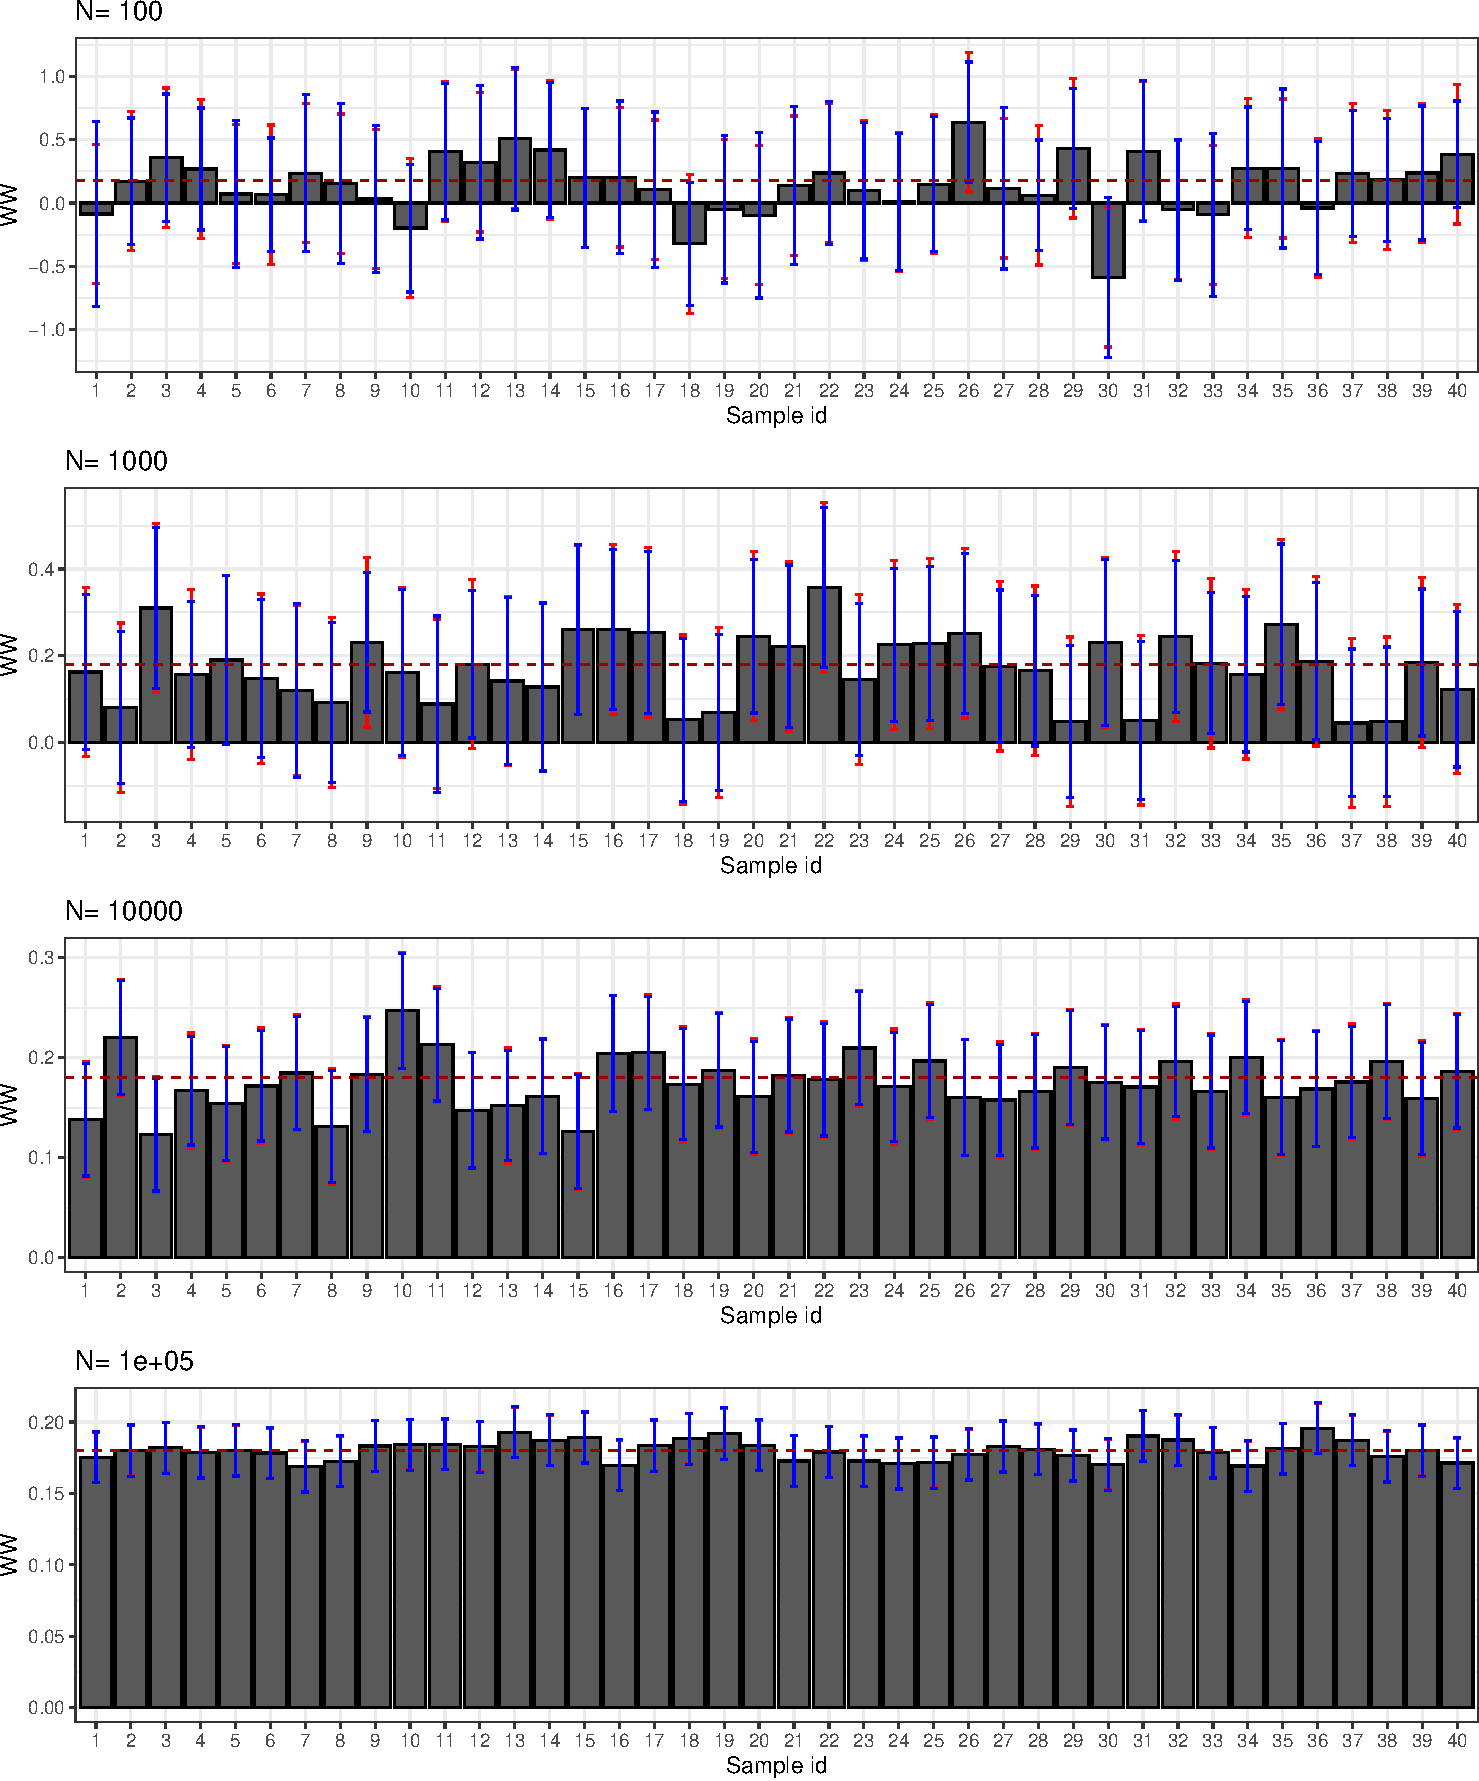
\includegraphics[width=0.6\linewidth]{STCI_files/figure-latex/confintervalCLT-1} 

}

\caption{CLT-based confidence intervals of $\hat{WW}$ for $\delta=$ 0.99 over sample replications for various sample sizes (true confidence intervals in red)}\label{fig:confintervalCLT}
\end{figure}

\BeginKnitrBlock{remark}
\iffalse{} {Remark. } \fi{}In proving the main result on the asymptotic distribution of \(\hat{WW}\), we have also proved a very useful result: \(\hat{WW}\) is the Ordinary Least Squares (OLS) estimator of \(\beta\) in the regression \(Y_i=\alpha+\beta D_i + U_i\).
This is pretty cool since we now can use our classical OLS estimator in our statistical package to estimate \(\hat{WW}\).
Let's compute the OLS estimate of \(WW\) in our sample:
\EndKnitrBlock{remark}

\begin{Shaded}
\begin{Highlighting}[]
\NormalTok{ols.ww <-}\StringTok{ }\KeywordTok{lm}\NormalTok{(y}\OperatorTok{~}\NormalTok{Ds)}
\NormalTok{ww.ols <-}\StringTok{ }\NormalTok{ols.ww}\OperatorTok{$}\NormalTok{coef[[}\DecValTok{2}\NormalTok{]]}
\end{Highlighting}
\end{Shaded}

We have \(\hat{WW}_{OLS}=\) 0.13 \(=\) 0.13 \(=\hat{WW}\).

\BeginKnitrBlock{remark}
\iffalse{} {Remark. } \fi{}Another pretty cool consequence of Theorem \ref{thm:asympnoiseWW} and of its proof is that the standard error of the OLS estimator of \(\hat{WW}\) (\(\sigma_{\beta}\)) is related to the sampling noise of \(\hat{WW}\) by the following formula:
\(2\tilde{\epsilon}=2\Phi^{-1}\left(\frac{\delta+1}{2}\right)\sigma_{\beta}\).
\EndKnitrBlock{remark}

This implies that sampling noise is equal to 5 \(\sigma_{\beta}\) when \(\delta=\) 0.99 and to 4 \(\sigma_{\beta}\) when \(\delta=\) 0.95.
It is thus very easy to move from estimates of the standard error of the \(\beta\) coefficient to the extent of sampling noise.

\BeginKnitrBlock{remark}
\iffalse{} {Remark. } \fi{}A last important consequence of Theorem \ref{thm:asympnoiseWW} and of its proof is that the standard error of the OLS estimator of \(\hat{WW}\) (\(\sigma_{\beta}\)) that we use is the heteroskedasticity-robust one.
\EndKnitrBlock{remark}

Using the RCM, we can indeed show that:

\begin{align*}
    \alpha & = \esp{Y_i^0|D_i=0}  \\
    \beta  & =  \Delta^Y_{TT} \\
    U_i    & = Y^0_i-\esp{Y^0_i|D_i=0} + D_i(\Delta^Y_i-\Delta^Y_{TT}),
    \end{align*}

Under Assumption \ref{def:noselb}, we have:

\begin{align*}
    U_i    & = (1-D_i)(Y^0_i-\esp{Y^0_i|D_i=0}) + D_i(Y_i^1-\esp{Y^1_i|D_i=1})
  \end{align*}

There is heteroskedasticity because the outcomes of the treated and of the untreated have different variances:

\begin{align*}
    \var{U_i|D_i=d} & = \esp{U_i^2|D_i=d}  \\
                    & = \esp{(Y^d_i-\esp{Y^d_i|D_i=d})^2|D_i=d}  \\
                    & = \var{Y_i^d|D_i=d}
  \end{align*}

We do not want to assume homoskedasticity, since it would imply a constant treatment effect.
Indeed, \(\var{Y_i^1|D_i=1} = \var{Y_i^0|D_i=1}+\var{\alpha_i|D_i=1}\).

\BeginKnitrBlock{remark}
\iffalse{} {Remark. } \fi{}In order to estimate the heteroskedasticity robust standard error from the OLS regression, we can use the sandwich package in R
Most available heteroskedasticity robust estimators based on the CLT can be written in the following way:
\EndKnitrBlock{remark}

\begin{align*}
  \var{\hat{\Theta}_{OLS}} & \approx (X'X)^{-1}X'\hat{\Omega}X(X'X)^{-1},
\end{align*}

where \(X\) is the matrix of regressors and \(\hat{\Omega}=\diag(\hat{\sigma}^2_{U_1},\dots,\hat{\sigma}^2_{U_N})\) is an estimate the covariance matrix of the residuals \(U_i\).
Here are various classical estimators for \(\hat{\Omega}\):

\begin{align*}
  \text{HC0:} & & \hat{\sigma_{U_i}}^2 & = \hat{U_i}^2 \\
  \text{HC1:} & & \hat{\sigma_{U_i}}^2 & = \frac{N}{N-K}\hat{U_i}^2 \\
  \text{HC2:} & & \hat{\sigma_{U_i}}^2 & = \frac{\hat{U_i}^2}{1-h_i} \\
  \text{HC3:} & & \hat{\sigma_{U_i}}^2 & = \frac{\hat{U_i}^2}{(1-h_i)^2}, 
\end{align*}

where \(\hat{U}_i\) is the residual from the OLS regression, \(K\) is the number of regressors, \(h_i\) is the leverage of observation \(i\), and is the \(i^{\text{th}}\) diagonal element of \(H=X(X'X)^{-1}X'\).
HC1 is the one reported by Stata when using the `robust' option.

\BeginKnitrBlock{example}
\protect\hypertarget{exm:unnamed-chunk-54}{}{\label{exm:unnamed-chunk-54} }Using the sandwich package, we can estimate the heteroskedasticity-robust variance-covariance matrix and sampling noise as follows:
\EndKnitrBlock{example}

\begin{Shaded}
\begin{Highlighting}[]
\NormalTok{ols.ww.vcov.HC0 <-}\StringTok{ }\KeywordTok{vcovHC}\NormalTok{(ols.ww, }\DataTypeTok{type =} \StringTok{"HC0"}\NormalTok{)}
\NormalTok{samp.noise.ww.CLT.ols <-}\StringTok{ }\ControlFlowTok{function}\NormalTok{(delta,reg,...)\{}
  \KeywordTok{return}\NormalTok{(}\DecValTok{2}\OperatorTok{*}\KeywordTok{qnorm}\NormalTok{((delta}\OperatorTok{+}\DecValTok{1}\NormalTok{)}\OperatorTok{/}\DecValTok{2}\NormalTok{)}\OperatorTok{*}\KeywordTok{sqrt}\NormalTok{(}\KeywordTok{vcovHC}\NormalTok{(reg,...)[}\DecValTok{2}\NormalTok{,}\DecValTok{2}\NormalTok{]))}
\NormalTok{\}}
\end{Highlighting}
\end{Shaded}

For \(\delta=\) 0.99, sampling noise estimated using the ``HC0'' option is equal to 0.35.
This is exactly the value we have estimated using our CLT-based formula (\(\hat{2\tilde{\epsilon}}=\) 0.35).
Remember that sampling noise is actually equal to 0.39.
Other ``HC'' options might be better in small samples.
For example, with the ``HC1'' option, we have an estimate for sampling noise of 0.35.
What would have happened to our estimate of sampling noise if we had ignored heteroskedasticity?
The default OLS standard error estimate yields an estimate for sampling noise of 0.36.

\hypertarget{sec:resamp}{%
\subsection{Using resampling methods}\label{sec:resamp}}

\hypertarget{sec:Fisher}{%
\subsection{Using randomization inference}\label{sec:Fisher}}

\hypertarget{part-methods-of-causal-inference}{%
\part{Methods of Causal Inference}\label{part-methods-of-causal-inference}}

\hypertarget{RCT}{%
\chapter{Randomized Controlled Trials}\label{RCT}}

\hypertarget{NE}{%
\chapter{Natural Experiments}\label{NE}}

\hypertarget{OM}{%
\chapter{Observational Methods}\label{OM}}

\hypertarget{part-additional-topics}{%
\part{Additional Topics}\label{part-additional-topics}}

\hypertarget{Power}{%
\chapter{Power Analysis}\label{Power}}

\hypertarget{Placebo}{%
\chapter{Placebo Tests}\label{Placebo}}

\hypertarget{cluster}{%
\chapter{Clustering}\label{cluster}}

\hypertarget{LaLonde}{%
\chapter{LaLonde Tests}\label{LaLonde}}

\hypertarget{Diffusion}{%
\chapter{Diffusion effects}\label{Diffusion}}

\hypertarget{Distribution}{%
\chapter{Distributional effects}\label{Distribution}}

\hypertarget{meta-analysis-and-publication-bias}{%
\chapter{Meta-analysis and Publication Bias}\label{meta-analysis-and-publication-bias}}

\hypertarget{Bounds}{%
\chapter{Bounds}\label{Bounds}}

\hypertarget{appendix-appendix}{%
\appendix}


\hypertarget{proofs}{%
\chapter{Proofs}\label{proofs}}

\hypertarget{proofs-of-results-in-chapter-reffpsi}{%
\section{Proofs of results in Chapter \ref{FPSI}}\label{proofs-of-results-in-chapter-reffpsi}}

\hypertarget{proofcheb}{%
\subsection{Proof of Theorem \ref{thm:uppsampnoise}}\label{proofcheb}}

In order to use Theorem \ref{thm:cheb} for studying the behavior of \(\hat{\Delta^Y_{WW}}\), we have to prove that it is unbiased and we have to compute \(\var{\hat{\Delta^Y_{WW}}}\).
Let's first prove that the \(WW\) estimator is an unbiased estimator of \(TT\):

\BeginKnitrBlock{lemma}[Unbiasedness of $\hat{\Delta^Y_{WW}}$]
\protect\hypertarget{lem:unbiasww}{}{\label{lem:unbiasww} \iffalse (Unbiasedness of \(\hat{\Delta^Y_{WW}}\)) \fi{} }Under Assumptions \ref{def:noselb}, \ref{def:fullrank} and \ref{def:iid},

\begin{align*}
\esp{\hat{\Delta^Y_{WW}}}& = \Delta^Y_{TT}.
\end{align*}
\EndKnitrBlock{lemma}

\BeginKnitrBlock{proof}
\iffalse{} {Proof. } \fi{}In order to prove Lemma \ref{lem:unbiasww}, we are going to use a trick.
We are going to compute the expectation of the \(WW\) estimator conditional on a given treatment allocation.
Because the resulting estimate is independent of treatment allocation, we will have our proof.
This trick simplifies derivations a lot and is really natural: think first of all the samples with the same treatment allocation, then average your results over all possible treatment allocations.

\begin{align*}
\esp{\hat{\Delta^Y_{WW}}} & = \esp{\esp{\hat{\Delta^Y_{WW}}|\mathbf{D}}}\\
                          & = \esp{\esp{\frac{1}{\sum_{i=1}^N D_i}\sum_{i=1}^N Y_iD_i-\frac{1}{\sum_{i=1}^N (1-D_i)}\sum_{i=1}^N Y_i(1-D_i)|\mathbf{D}}}\\
                          & = \esp{\esp{\frac{1}{\sum_{i=1}^N D_i}\sum_{i=1}^N Y_iD_i|\mathbf{D}}-\esp{\frac{1}{\sum_{i=1}^N (1-D_i)}\sum_{i=1}^N Y_i(1-D_i)|\mathbf{D}}}\\
                          & = \esp{\frac{1}{\sum_{i=1}^N D_i}\esp{\sum_{i=1}^N Y_iD_i|\mathbf{D}}-\frac{1}{\sum_{i=1}^N (1-D_i)}\esp{\sum_{i=1}^N Y_i(1-D_i)|\mathbf{D}}}\\
                          & = \esp{\frac{1}{\sum_{i=1}^N D_i}\sum_{i=1}^N \esp{Y_iD_i|\mathbf{D}}-\frac{1}{\sum_{i=1}^N (1-D_i)}\sum_{i=1}^N \esp{Y_i(1-D_i)|\mathbf{D}}}\\
                          & = \esp{\frac{1}{\sum_{i=1}^N D_i}\sum_{i=1}^N \esp{Y_iD_i|D_i}-\frac{1}{\sum_{i=1}^N (1-D_i)}\sum_{i=1}^N \esp{Y_i(1-D_i)|D_i}}\\
                          & = \esp{\frac{1}{\sum_{i=1}^N D_i}\sum_{i=1}^N D_i\esp{Y_i|D_i=1}-\frac{1}{\sum_{i=1}^N (1-D_i)}\sum_{i=1}^N(1-D_i)\esp{Y_i|D_i=0}}\\
                          & = \esp{\frac{\sum_{i=1}^N D_i}{\sum_{i=1}^N D_i}\esp{Y_i|D_i=1}-\frac{\sum_{i=1}^N(1-D_i)}{\sum_{i=1}^N (1-D_i)}\esp{Y_i|D_i=0}}\\
                          & = \esp{\esp{Y_i|D_i=1}-\esp{Y_i|D_i=0}}\\
                          & = \esp{Y_i|D_i=1}-\esp{Y_i|D_i=0} \\
                          & = \Delta^Y_{TT}.
\end{align*}

The first equality uses the Law of Iterated Expectations (LIE).
The second and fourth equalities use the linearity of conditional expectations.
The third equality uses the fact that, conditional on \(\mathbf{D}\), the number of treated and untreated is a constant.
The fifth equality uses Assumption \ref{def:iid}.
The sixth equality uses the fact that \(\esp{Y_iD_i|D_i}=D_i\esp{Y_i*1|D_i=1}+(1-D_i)\esp{Y_i*0|D_i=0}\).
The seventh and ninth equalities use the fact that \(\esp{Y_i|D_i=1}\) is a constant.
The last equality uses Assumption \ref{def:noselb}.
\EndKnitrBlock{proof}

Let's now compute the variance of the \(WW\) estimator:

\BeginKnitrBlock{lemma}[Variance of $\hat{\Delta^Y_{WW}}$]
\protect\hypertarget{lem:varww}{}{\label{lem:varww} \iffalse (Variance of \(\hat{\Delta^Y_{WW}}\)) \fi{} }Under Assumptions \ref{def:noselb}, \ref{def:fullrank} and \ref{def:iid},

\begin{align*}
\var{{\hat{\Delta^Y_{WW}}}} & = \frac{1-(1-\Pr(D_i=1))^N}{N\Pr(D_i=1)}\var{Y_i^1|D_i=1}+\frac{1-\Pr(D_i=1)^N}{N(1-\Pr(D_i=1))}\var{Y_i^0|D_i=0}.
\end{align*}
\EndKnitrBlock{lemma}

\BeginKnitrBlock{proof}
\iffalse{} {Proof. } \fi{}Same trick as before, but now using the Law of Total Variance (LTV):

\begin{align*}
\var{{\hat{\Delta^Y_{WW}}}} & = \esp{\var{\hat{\Delta^Y_{WW}}|\mathbf{D}}}+\var{\esp{\hat{\Delta^Y_{WW}}|\mathbf{D}}}\\
                            & = \esp{\var{\frac{1}{\sum_{i=1}^N D_i}\sum_{i=1}^N Y_iD_i-\frac{1}{\sum_{i=1}^N (1-D_i)}\sum_{i=1}^N Y_i(1-D_i)|\mathbf{D}}} \\
                            & = \esp{\var{\frac{1}{\sum_{i=1}^N D_i}\sum_{i=1}^N Y_iD_i|\mathbf{D}}}+\esp{\var{\frac{1}{\sum_{i=1}^N (1-D_i)}\sum_{i=1}^N Y_i(1-D_i)|\mathbf{D}}}\\
                            & \phantom{=}+\esp{\cov{\frac{1}{\sum_{i=1}^N D_i}\sum_{i=1}^N Y_iD_i,\frac{1}{\sum_{i=1}^N (1-D_i)}\sum_{i=1}^N Y_i(1-D_i)|\mathbf{D}}} \\
                            & = \esp{\frac{1}{(\sum_{i=1}^N D_i)^2}\var{\sum_{i=1}^N Y_iD_i|\mathbf{D}}}+\esp{\frac{1}{(\sum_{i=1}^N (1-D_i))^2}\var{\sum_{i=1}^N Y_i(1-D_i)|\mathbf{D}}} \\
                            & = \esp{\frac{1}{(\sum_{i=1}^N D_i)^2}\var{\sum_{i=1}^N Y_iD_i|D_i}}+\esp{\frac{1}{(\sum_{i=1}^N (1-D_i))^2}\var{\sum_{i=1}^N Y_i(1-D_i)|D_i}} \\
                            & = \esp{\frac{1}{(\sum_{i=1}^N D_i)^2}\sum_{i=1}^ND_i\var{Y_i|D_i=1}}+\esp{\frac{1}{(\sum_{i=1}^N (1-D_i))^2}\sum_{i=1}^N(1-D_i)\var{Y_i|D_i=0}} \\
                            & = \var{Y_i|D_i=1}\esp{\frac{1}{\sum_{i=1}^N D_i}}+\var{Y_i|D_i=0}\esp{\frac{1}{\sum_{i=1}^N (1-D_i)}} \\
                            & = \frac{1-(1-\Pr(D_i=1))^N}{N\Pr(D_i=1)}\var{Y_i^1|D_i=1}+\frac{1-\Pr(D_i=1)^N}{N(1-\Pr(D_i=1))}\var{Y_i^0|D_i=0}.
\end{align*}

The first equality stems from the LTV.
The second and third equalities stems from the definition of the \(WW\) estimator and of the variance of a sum of random variables.
The fourth equality stems from Assumption \ref{def:iid}, which means that the covariance across observations is zero, and from the formula for a variance of a random variable multiplied by a constant.
The fifth and sixth equalities stems from Assumption \ref{def:iid} and from \(\var{Y_iD_i|D_i}=D_i\var{Y_i*1|D_i=1}+(1-D_i)\var{Y_i*0|D_i=0}\).
The seventh equality stems from \(\var{Y_i|D_i=1}\) and \(\var{Y_i|D_i=0}\) being constant.
The last equality stems from the formula for the expectation of the inverse of a sum of Bernoulli random variables with at least one of them taking value one which is the case under Assumption \ref{def:fullrank}.
\EndKnitrBlock{proof}

Using Theorem \ref{thm:cheb}, we have:

\begin{align*}
2\epsilon & \leq 2\sqrt{\frac{1}{N(1-\delta)}\left(\frac{1-(1-\Pr(D_i=1))^N}{\Pr(D_i=1)}\var{Y_i^1|D_i=1}+\frac{1-\Pr(D_i=1)^N}{(1-\Pr(D_i=1))}\var{Y_i^0|D_i=0}\right)}\\
          & \leq 2\sqrt{\frac{1}{N(1-\delta)}\left(\frac{\var{Y_i^1|D_i=1}}{\Pr(D_i=1)}+\frac{\var{Y_i^0|D_i=0}}{(1-\Pr(D_i=1))}\right)},
\end{align*}

where the second equality stems from the fact that \(\frac{(1-\Pr(D_i=1))^N}{\Pr(D_i=1)}\var{Y_i^1|D_i=1}+\frac{\Pr(D_i=1)^N}{(1-\Pr(D_i=1))}\var{Y_i^0|D_i=0}\geq0\).
This proves the result.

\hypertarget{proofCLT}{%
\subsection{Proof of Theorem \ref{thm:asympnoiseWW}}\label{proofCLT}}

Before proving Theorem \ref{thm:asympnoiseWW}, let me state a very useful result: \(\hat{WW}\) can be computed using OLS:

\BeginKnitrBlock{lemma}[WW is OLS]
\protect\hypertarget{lem:WWOLS}{}{\label{lem:WWOLS} \iffalse (WW is OLS) \fi{} }Under Assumption \ref{def:fullrank}, the OLS coefficient \(\beta\) in the following regression:

\begin{align*}
        Y_i &  = \alpha +  \beta D_i + U_i
    \end{align*}

is the WW estimator:

\begin{align*}
\hat{\beta}_{OLS} & = \frac{\frac{1}{N}\sum_{i=1}^N\left(Y_i-\frac{1}{N}\sum_{i=1}^NY_i\right)\left(D_i-\frac{1}{N}\sum_{i=1}^ND_i\right)}{\frac{1}{N}\sum_{i=1}^N\left(D_i-\frac{1}{N}\sum_{i=1}^ND_i\right)^2} \\
                                & = \hat{\Delta^Y_{WW}}.
\end{align*}
\EndKnitrBlock{lemma}

\BeginKnitrBlock{proof}
\iffalse{} {Proof. } \fi{}In matrix notation, we have:

\begin{align*}
  \underbrace{\left(\begin{array}{c}  Y_1 \\    \vdots \\   Y_N \end{array}\right)}_{Y} & = 
  \underbrace{\left(\begin{array}{cc}   1 & D_1\\   \vdots & \vdots\\   1 & D_N\end{array}\right)}_{X}
  \underbrace{\left(\begin{array}{c}    \alpha \\   \beta \end{array}\right)}_{\Theta}+
  \underbrace{\left(\begin{array}{c}    U_1 \\  \vdots \\   U_N \end{array}\right)}_{U}
\end{align*}

The OLS estimator is:

\begin{align*}
    \hat{\Theta}_{OLS} &  = (X'X)^{-1}X'Y
\end{align*}

Under the Full Rank Assumption, \(X'X\) is invertible and we have:

\begin{align*}
(X'X)^{-1} &  = \left(\begin{array}{cc} N & \sum_{i=1}^ND_i \\ \sum_{i=1}^ND_i & \sum_{i=1}^ND_i^2 \end{array}\right)^{-1} \\
                & = \frac{1}{N\sum_{i=1}^ND_i^2-\left(\sum_{i=1}^ND_i\right)^2}\left(\begin{array}{cc} \sum_{i=1}^ND_i^2 & -\sum_{i=1}^ND_i \\ -\sum_{i=1}^ND_i & N \end{array}\right)
\end{align*}

For simplicity, I omit the summation index:

\begin{align*}
  \hat{\Theta}_{OLS} &  = \frac{1}{N\sum D_i^2-\left(\sum D_i\right)^2}
                          \left(\begin{array}{cc} \sum D_i^2 & -\sum D_i \\ -\sum D_i & N \end{array}\right)
                          \left(\begin{array}{c} \sum Y_i \\  \sum Y_iD_i \end{array}\right) \\
                    & = \frac{1}{N\sum D_i^2-\left(\sum D_i\right)^2}
                        \left(\begin{array}{c} \sum D_i^2\sum Y_i-\sum D_i\sum_{i=1}^NY_iD_i \\
                                              -\sum D_i\sum Y_i+ N\sum Y_iD_i \end{array}\right) \\
\end{align*}

Using \(D_i^2=D_i\), we have:

\begin{align*}
  \hat{\Theta}_{OLS} &  =  \left(\begin{array}{c} 
          \frac{\left(\sum D_i\right)\left(\sum Y_i-\sum Y_iD_i\right)}{\left(\sum D_i\right)\left(N-\sum D_i\right)} \\
          \frac{N\sum Y_iD_i-\sum D_i\sum Y_i}{N\sum D_i-\left(\sum D_i\right)^2} 
                            \end{array}\right) 
                        =     \left(\begin{array}{c} 
          \frac{\sum (Y_iD_i+Y_i(1-D_i))-\sum Y_iD_i}{\sum(1-D_i)} \\
          \frac{N^2}{N^2}\frac{\frac{1}{N}\sum Y_iD_i-\frac{1}{N}\sum D_i\frac{1}{N}\sum Y_i+\frac{1}{N}\sum D_i\frac{1}{N}\sum Y_i-\frac{1}{N}\sum D_i\frac{1}{N}\sum Y_i}{\frac{1}{N}\sum D_i-2\left(\frac{1}{N}\sum D_i\right)^2+\left(\frac{1}{N}\sum D_i\right)^2} 
                            \end{array}\right) \\
                      &  =     \left(\begin{array}{c} 
          \frac{\sum Y_i(1-D_i)}{\sum(1-D_i)} \\
          \frac{\frac{1}{N}\sum \left(Y_iD_i-D_i\frac{1}{N}\sum Y_i-Y_i\frac{1}{N}\sum D_i+\frac{1}{N}\sum D_i\frac{1}{N}\sum Y_i\right)}{\frac{1}{N}\sum\left(D_i-2D_i\frac{1}{N}\sum D_i+\left(\frac{1}{N}\sum D_i\right)^2\right)} 
                            \end{array}\right) 
                      =     \left(\begin{array}{c} 
          \frac{\sum Y_i(1-D_i)}{\sum(1-D_i)} \\
    \frac{\frac{1}{N}\sum\left(Y_i-\frac{1}{N}\sum Y_i\right)\left(D_i-\frac{1}{N}\sum D_i\right)}{\frac{1}{N}\sum \left(D_i-\frac{1}{N}\sum D_i\right)^2} 
                            \end{array}\right), 
\end{align*}

which proves the first part of the lemma.
Now for the second part of the lemma:

\begin{align*}
  \hat{\beta}_{OLS} &  = \frac{\sum Y_iD_i-\frac{1}{N}\sum D_i\sum Y_i}{\sum D_i\left(1-\frac{1}{N}\sum D_i\right)}
                       = \frac{\sum Y_iD_i-\frac{1}{N}\sum D_i\sum\left(Y_iD_i+(1-D_i)Y_i\right)}{\sum D_i\left(1-\frac{1}{N}\sum D_i\right)}\\
                    &  = \frac{\sum Y_iD_i\left(1-\frac{1}{N}\sum D_i\right)-\frac{1}{N}\sum D_i\sum(1-D_i)Y_i}{\sum D_i\left(1-\frac{1}{N}\sum D_i\right)}\\
                    &  = \frac{\sum Y_iD_i}{\sum D_i}-\frac{\frac{1}{N}\sum(1-D_i)Y_i}{\left(1-\frac{1}{N}\sum D_i\right)}\\
                    &  = \frac{\sum Y_iD_i}{\sum D_i}-\frac{\frac{1}{N}\sum(1-D_i)Y_i}{\frac{1}{N}\sum\left(1-D_i\right)}\\
                     &  = \frac{\sum Y_iD_i}{\sum D_i}-\frac{\sum(1-D_i)Y_i}{\sum\left(1-D_i\right)}\\
                     & = \hat{\Delta^Y_{WW}},
\end{align*}

which proves the result.
\EndKnitrBlock{proof}

Now, let me state the most important lemma behind the result in Theorem \ref{thm:asympnoiseWW}:

\BeginKnitrBlock{lemma}[Asymptotic Distribution of the OLS Estimator]
\protect\hypertarget{lem:asympOLS}{}{\label{lem:asympOLS} \iffalse (Asymptotic Distribution of the OLS Estimator) \fi{} }Under Assumptions \ref{def:noselb}, \ref{def:fullrank}, \ref{def:iid} and \ref{def:finitevar}, we have:

\begin{align*}
  \sqrt{N}(\hat{\Theta}_{OLS}-\Theta) &  \stackrel{d}{\rightarrow}
  \mathcal{N}\left(\begin{array}{c} 0\\ 0\end{array},
  \sigma_{XX}^{-1}\mathbf{V_{xu}}\sigma_{XX}^{-1}\right), 
\end{align*}

with
\begin{align*}
\sigma_{XX}^{-1}& = \left(\begin{array}{cc} \frac{\Pr(D_i=1)}{\Pr(D_i=1)(1-\Pr(D_i=1))} & -\frac{\Pr(D_i=1)}{\Pr(D_i=1)(1-\Pr(D_i=1))}\\
                                          -\frac{\Pr(D_i=1)}{\Pr(D_i=1)(1-\Pr(D_i=1))} & \frac{1}{\Pr(D_i=1)(1-\Pr(D_i=1))} 
                          \end{array}\right)\\
\mathbf{V_{xu}}&= \esp{U_i^2\left(\begin{array}{cc}  1 & D_i\\  D_i & D_i\end{array}\right)}                        
\end{align*}
\EndKnitrBlock{lemma}

\BeginKnitrBlock{proof}
\iffalse{} {Proof. } \fi{}
\begin{align*}
\sqrt{N}(\hat{\Theta}_{OLS}-\Theta) & = \sqrt{N}((X'X)^{-1}X'Y-\Theta) \\
                                    & = \sqrt{N}((X'X)^{-1}X'(X\Theta+U)-\Theta) \\
                                    & = \sqrt{N}((X'X)^{-1}X'X\Theta+(X'X)^{-1}X'U)-\Theta) \\
                                    & = \sqrt{N}(X'X)^{-1}X'U \\
                                    & = N(X'X)^{-1}\frac{\sqrt{N}}{N}X'U
\end{align*}

Using Slutsky's Theorem, we can study both terms separately.
Slutsky's Theorem states that if \(Y_N\stackrel{d}{\rightarrow}y\) and \(\text{plim}(X_N)=x\), then:

\begin{enumerate}
\def\labelenumi{\arabic{enumi}.}
\tightlist
\item
  \(X_N+Y_N\stackrel{d}{\rightarrow}x+y\)
\item
  \(X_NY_N\stackrel{d}{\rightarrow}xy\)
\item
  \(\frac{Y_N}{X_N}\stackrel{d}{\rightarrow}\frac{x}{y}\) if \(x\neq0\)
\end{enumerate}

Using this theorem, we have:

\begin{align*}
\sqrt{N}(\hat{\Theta}_{OLS}-\Theta) & \stackrel{d}{\rightarrow} \sigma_{XX}^{-1}xu,
\end{align*}

Where \(\sigma_{XX}^{-1}\) is a matrix of constants and \(xu\) is a random variable.

Let's begin with \(\frac{\sqrt{N}}{N}X'U\stackrel{d}{\rightarrow}xu\):

\begin{align*}
\frac{\sqrt{N}}{N}X'U & = \sqrt{N}\left(\begin{array}{c}  \frac{1}{N}\sum^{i=1}_{N}U_i\\  \frac{1}{N}\sum^{i=1}_{N}D_iU_i\end{array}\right)
\end{align*}

In order to determine the asymptotic distribution of \(\frac{\sqrt{N}}{N}X'U\), we are going to use the vector version of the CLT:

If \(X_i\) and \(Y_i\) are two i.i.d. random variables with finite first and second moments, we have:

\begin{align*}
    \sqrt{N}
  \left(
      \begin{array}{c}  
       \frac{1}{N}\sum_{i=1}^NX_i-\esp{X_i}\\   
       \frac{1}{N}\sum_{i=1}^NY_i-\esp{Y_i}
       \end{array}
     \right) 
      &
  \stackrel{d}{\rightarrow}
  \mathcal{N}
  \left(
    \begin{array}{c}    
    0\\
    0
    \end{array},
  \mathbf{V}
  \right),
\end{align*}

where \(\mathbf{V}\) is the population covariance matrix of \(X_i\) and \(Y_i\).

We know that, under Assumption \ref{def:noselb}, both random variables have mean zero:

\begin{align*}
\esp{U_i}& = \esp{U_i|D_i=1}\Pr(D_i=1)+\esp{U_i|D_i=0}\Pr(D_i=0)=0 \\
\esp{U_iD_i}& = \esp{U_i|D_i=1}\Pr(D_i=1)=0
\end{align*}

Their covariance matrix \(\mathbf{V_{xu}}\) can be computed as follows:

\begin{align*}
\mathbf{V_{xu}} & = \esp{\left(\begin{array}{c}  U_i\\  UiD_i\end{array}\right)\left(\begin{array}{cc}  U_i&    UiD_i\end{array}\right)}
                  - \esp{\left(\begin{array}{c} U_i\\   UiD_i\end{array}\right)}\esp{\left(\begin{array}{cc}    U_i&    UiD_i\end{array}\right)}\\
                & = \esp{\left(\begin{array}{cc}    U_i^2 & U_i^2D_i\\  Ui^2D_i & U_i^2D_i^2\end{array}\right)} 
                  = \esp{U_i^2\left(\begin{array}{cc}   1 & D_i\\   D_i & D_i^2\end{array}\right)} 
                  = \esp{U_i^2\left(\begin{array}{cc}   1 & D_i\\   D_i & D_i\end{array}\right)} 
\end{align*}

Using the Vector CLT, we have that \(\frac{\sqrt{N}}{N}X'U\stackrel{d}{\rightarrow}\mathcal{N}\left(\begin{array}{c} 0\\ 0\end{array},\mathbf{V_{xu}}\right)\).

Let's show now that \(\plims N(X'X)^{-1}=\sigma_{XX}^{-1}\):

\begin{align*}
N(X'X)^{-1} & = \frac{N}{N\sum_{i=1}^ND_i-\left(\sum_{i=1}^ND_i\right)^2}
                \left(\begin{array}{cc} \sum_{i=1}^ND_i & -\sum_{i=1}^ND_i \\ -\sum_{i=1}^ND_i & N \end{array}\right) \\
            & = \frac{1}{N}\frac{1}{\frac{1}{N}\sum_{i=1}^ND_i-\left(\frac{1}{N}\sum_{i=1}^ND_i\right)^2}
                \left(\begin{array}{cc} \sum_{i=1}^ND_i & -\sum_{i=1}^ND_i \\ -\sum_{i=1}^ND_i & N \end{array}\right)\\
            & = \frac{1}{\frac{1}{N}\sum_{i=1}^ND_i-\left(\frac{1}{N}\sum_{i=1}^ND_i\right)^2}
                \left(\begin{array}{cc} \frac{1}{N}\sum_{i=1}^ND_i & -\frac{1}{N}\sum_{i=1}^ND_i \\ -\frac{1}{N}\sum_{i=1}^ND_i & 1 \end{array}\right)\\
\plims N(X'X)^{-1} & = \frac{1}{\plims\frac{1}{N}\sum_{i=1}^ND_i-\left(\plims\frac{1}{N}\sum_{i=1}^ND_i\right)^2}
                \left(\begin{array}{cc} \plims\frac{1}{N}\sum_{i=1}^ND_i & -\plims\frac{1}{N}\sum_{i=1}^ND_i \\ -\plims\frac{1}{N}\sum_{i=1}^ND_i & 1 \end{array}\right)\\
                  & = \frac{1}{\Pr(D_i=1)-\Pr(D_i=1)^2}
                \left(\begin{array}{cc} \Pr(D_i=1) & -\Pr(D_i=1) \\ -\Pr(D_i=1) & 1 \end{array}\right)\\
                 & = \sigma_{XX}^{-1}
\end{align*}

The fourth equality uses Slutsky's Theorem.
The fifth equality uses the Law of Large Numbers (LLN): if \(Y_i\) are i.i.d. variables with finite first and second moments, \(\plim{N}\frac{1}{N}\sum_{i=1}^NY_i = \esp{Y_i}\).

In order to complete the proof, we have to use the Delta Method Theorem.
This theorem states that:

\begin{gather*}
  \sqrt{N}(\begin{array}{c} \bar{X}_N-\esp{X_i}\\   \bar{Y}_N-\esp{Y_i}\end{array})  \stackrel{d}{\rightarrow}\mathcal{N}(\begin{array}{c}  0\\ 0\end{array},\mathbf{V}) \\
\Rightarrow \sqrt{N}(g(\bar{X}_N,\bar{Y}_N)-g(\esp{X_i},\esp{Y_i})  \stackrel{d}{\rightarrow}\mathcal{N}(0,G'\mathbf{V}G)
\end{gather*}

where \(G(u)=\partder{g(u)}{u}\) and \(G=G(\esp{X_i},\esp{Y_i})\).

In our case, \(g(xu)=\sigma_{XX}^{-1}xu\), so \(G(xu)=\sigma_{XX}^{-1}\).
The results follows from that and from the symmetry of \(\sigma_{XX}^{-1}\).
\EndKnitrBlock{proof}

A last lemma uses the previous result to derive the asymptotic distribution of \(\hat{WW}\):

\BeginKnitrBlock{lemma}[Asymptotic Distribution of $\hat{WW}$]
\protect\hypertarget{lem:asymWW}{}{\label{lem:asymWW} \iffalse (Asymptotic Distribution of \(\hat{WW}\)) \fi{} }Under Assumptions \ref{def:noselb}, \ref{def:fullrank}, \ref{def:iid} and \ref{def:finitevar}, we have:

\begin{align*}
  \sqrt{N}(\hat{\Delta^Y_{WW}}-\Delta^Y_{TT}) &  \stackrel{d}{\rightarrow}
  \mathcal{N}\left(0,\frac{\var{Y_i^1|D_i=1}}{\Pr(D_i=1)}+\frac{\var{Y_i^0|D_i=0}}{1-\Pr(D_i=1)}\right).
\end{align*}
\EndKnitrBlock{lemma}

\BeginKnitrBlock{proof}
\iffalse{} {Proof. } \fi{}In order to derive the asymptotic distribution of WW, I use first Lemma \ref{lem:WWOLS} which implies that the asymptotic distribution of WW is the same as that of \(\hat{\beta}_{OLS}\).
Now, from Lemma \ref{lem:asympOLS}, we know that \(\sqrt{N}(\hat{\beta}_{OLS}-\beta)\stackrel{d}{\rightarrow}\mathcal{N}(0,\sigma^2_{\beta})\), where \(\sigma^2_{\beta}\) is the lower diagonal term of \(\sigma_{XX}^{-1}\mathbf{V_{xu}}\sigma_{XX}^{-1}\).
Using the convention \(p=\Pr(D_i=1)\), we have:

\begin{align*}
\sigma_{XX}^{-1}\mathbf{V_{xu}}\sigma_{XX}^{-1} 
                  & = \left(\begin{array}{cc}  
                                          \frac{p}{p(1-p)} & -\frac{p}{p(1-p)}\\
                                          -\frac{p}{p(1-p)} & \frac{1}{p(1-p)} 
                          \end{array}\right)
                          \esp{U_i^2\left(\begin{array}{cc}  1 & D_i\\  D_i & D_i\end{array}\right)}        
                          \left(\begin{array}{cc}  
                                          \frac{p}{p(1-p)} & -\frac{p}{p(1-p)}\\
                                          -\frac{p}{p(1-p)} & \frac{1}{p(1-p)} 
                          \end{array}\right)\\
                  & = \frac{1}{(p(1-p))^2}
                          \left(\begin{array}{cc}  
                                          p\esp{U_i^2}-p\esp{U_i^2D_i} & p\esp{U_i^2D_i}-p\esp{U_i^2D_i}\\
                                          -p\esp{U_i^2}+\esp{U_i^2D_i} &  -p\esp{U_i^2D_i}+\esp{U_i^2D_i}
                          \end{array}\right)
                         \left(\begin{array}{cc}  
                                          p & -p\\
                                          -p & 1 
                          \end{array}\right)\\
                 & = \frac{1}{(p(1-p))^2}
                          \left(\begin{array}{cc}  
                                          p^2(\esp{U_i^2}-\esp{U_i^2D_i}) & p^2(\esp{U_i^2D_i}-\esp{U_i^2})\\
                                          p^2(\esp{U_i^2D_i}-\esp{U_i^2}) &  p^2\esp{U_i^2}+(1-2p)\esp{U_i^2D_i}
                          \end{array}\right)
 \end{align*}

The final result comes from the fact that:

\begin{align*}
\esp{U_i^2} & = \esp{U_i^2|D_i=1}p + (1-p)\esp{U_i^2|D_i=0}\\
            & = p\var{Y_i^1|D_i=1}+(1-p)\var{Y_i^0|D_i=0} \\
\esp{U_i^2D_i}  & = \esp{U_i^2|D_i=1}p  \\
                & = p\var{Y_i^1|D_i=1}.
 \end{align*}

As a consequence:

\begin{align*}
\sigma^2_{\beta} &= \frac{1}{(p(1-p))^2}\left(\var{Y_i^1|D_i=1}p(p^2-2p+1) + p^2(1-p)\var{Y_i^0|D_i=0}\right) \\
                  &= \frac{1}{(p(1-p))^2}\left(\var{Y_i^1|D_i=1}p(1-p)^2 + p^2(1-p)\var{Y_i^0|D_i=0}\right)\\
                  & = \frac{\var{Y_i^1|D_i=1}}{p}+\frac{\var{Y_i^0|D_i=0}}{1-p}.
 \end{align*}
\EndKnitrBlock{proof}

Using the previous lemma, we can now approximate the confidence level of \(\hat{WW}\):

\begin{align*}
\Pr&(|\hat{\Delta^Y_{WW}}-\Delta^Y_{TT}|\leq\epsilon) = \Pr(-\epsilon\leq\hat{\Delta^Y_{WW}}-\Delta^Y_{TT}\leq\epsilon) \\
& = \Pr\left(-\frac{\epsilon}{\frac{1}{\sqrt{N}}\sqrt{\frac{\var{Y_i^1|D_i=1}}{\Pr(D_i=1)}+\frac{\var{Y_i^0|D_i=0}}{1-\Pr(D_i=1)}}}\leq\frac{\hat{\Delta^Y_{WW}}-\Delta^Y_{TT}}{\frac{1}{\sqrt{N}}\sqrt{\frac{\var{Y_i^1|D_i=1}}{\Pr(D_i=1)}+\frac{\var{Y_i^0|D_i=0}}{1-\Pr(D_i=1)}}}\leq\frac{\epsilon}{\frac{1}{\sqrt{N}}\sqrt{\frac{\var{Y_i^1|D_i=1}}{\Pr(D_i=1)}+\frac{\var{Y_i^0|D_i=0}}{1-\Pr(D_i=1)}}}\right)\\
& \approx \Phi\left(\frac{\epsilon}{\frac{1}{\sqrt{N}}\sqrt{\frac{\var{Y_i^1|D_i=1}}{\Pr(D_i=1)}+\frac{\var{Y_i^0|D_i=0}}{1-\Pr(D_i=1)}}}\right)-
\Phi\left(-\frac{\epsilon}{\frac{1}{\sqrt{N}}\sqrt{\frac{\var{Y_i^1|D_i=1}}{\Pr(D_i=1)}+\frac{\var{Y_i^0|D_i=0}}{1-\Pr(D_i=1)}}}\right)\\
& = \Phi\left(\frac{\epsilon}{\frac{1}{\sqrt{N}}\sqrt{\frac{\var{Y_i^1|D_i=1}}{\Pr(D_i=1)}+\frac{\var{Y_i^0|D_i=0}}{1-\Pr(D_i=1)}}}\right)- 1 + \Phi\left(\frac{\epsilon}{\frac{1}{\sqrt{N}}\sqrt{\frac{\var{Y_i^1|D_i=1}}{\Pr(D_i=1)}+\frac{\var{Y_i^0|D_i=0}}{1-\Pr(D_i=1)}}}\right)\\
& = 2\Phi\left(\frac{\epsilon}{\frac{1}{\sqrt{N}}\sqrt{\frac{\var{Y_i^1|D_i=1}}{\Pr(D_i=1)}+\frac{\var{Y_i^0|D_i=0}}{1-\Pr(D_i=1)}}}\right)-1.
\end{align*}

As a consequence,

\begin{align*}
\delta & \approx 2\Phi\left(\frac{\epsilon}{\frac{1}{\sqrt{N}}\sqrt{\frac{\var{Y_i^1|D_i=1}}{\Pr(D_i=1)}+\frac{\var{Y_i^0|D_i=0}}{1-\Pr(D_i=1)}}}\right)-1.
\end{align*}

Hence the result.


\end{document}
